% =========================================================================
% mainV4.tex: the SUBMITTED mainV3 (CVPR 2027 #28592, Overleaf copy of 2026-11-17) with the
% supplementary sections re-ordered to follow the main paper. The main 8 pages (everything
% through the references and the S-numbering setup) are UNCHANGED from the submission and
% must stay frozen. Only the appendix was re-sequenced; see the banner comments A-L.
% =========================================================================
% =========================================================================
% mainV3.tex: built from mainV2.tex on 2026-11-14. Changes: rescoped title, experiments lead with rows, 'one pretraining, two specializations', two-stage result framed as an ablation, repetition cut, published-encoder comparison table in the main body.
% Previous title (mainV2): CropCode: Inverse Procedural Modeling of Occluded Row Crop Geometry from Sparse Multimodal Field Observations
% CVPR 2027 Submission — "CropCode: Inverse Procedural Modeling of Occluded Row Crop Geometry from Sparse Multimodal Field Observations"
% =========================================================================
\documentclass[10pt,twocolumn,letterpaper]{article}

%%%%%%%%% PAPER TYPE  - PLEASE UPDATE FOR FINAL VERSION
\usepackage[review]{cvpr}      % To produce the REVIEW version
% \usepackage{cvpr}              % To produce the CAMERA-READY version
% \usepackage[pagenumbers]{cvpr} % To force page numbers, e.g. for an arXiv version

% Chart colors
\definecolor{seriesF}{HTML}{2A78D6}
\definecolor{seriesP}{HTML}{1BAF7A}
\definecolor{seriesR}{HTML}{4A3AA7}
\definecolor{gridc}{HTML}{E4E3DF}
\definecolor{axisc}{HTML}{52514E}

\definecolor{cLegRed}{HTML}{D62728}%
\definecolor{cLegOrange}{HTML}{FF8C00}%
\definecolor{cLegGreen}{HTML}{2CA02C}%

\usepackage{tikz}
\usepackage{pgfplots}
\pgfplotsset{compat=1.18}
\usetikzlibrary{arrows.meta}

% Contact-solver pseudocode
\usepackage{algorithm}
\usepackage[noend]{algpseudocode}
\algrenewcommand\algorithmiccomment[1]{\hfill{\footnotesize\textcolor{black!60}{$\triangleright$ #1}}}
\newcommand{\Meets}{\textsc{Meets}}

% Formatting & layout tweaks
\usepackage{microtype}
\usepackage{placeins} % \FloatBarrier
\renewcommand{\dbltopfraction}{0.99}

% Keep revision macros as clean no-ops for compatibility
\newcommand{\upd}[1]{#1}
\newcommand{\updtwo}[1]{#1}

% Hyperref setup
\definecolor{cvprblue}{rgb}{0.21,0.49,0.74}
\usepackage[pagebackref,breaklinks,colorlinks,allcolors=cvprblue]{hyperref}

% ---- Cross-reference macros: the whole phrase ("Fig. 3") is the colored link
\newcommand{\figref}[1]{\hyperref[#1]{Fig.~\ref*{#1}}}
\newcommand{\Figref}[1]{\hyperref[#1]{Figure~\ref*{#1}}}
\newcommand{\subfigref}[2]{\hyperref[#1]{Fig.~\ref*{#1}#2}} % panel: \subfigref{fig:x}{A} -> Fig. S5A
\newcommand{\tabref}[1]{\hyperref[#1]{Table~\ref*{#1}}}
\newcommand{\secref}[1]{\hyperref[#1]{Sec.~\ref*{#1}}}
\newcommand{\Secref}[1]{\hyperref[#1]{Section~\ref*{#1}}}
\newcommand{\appendixref}[1]{\hyperref[#1]{Appendix~\ref*{#1}}}
\PassOptionsToPackage{nameinlink}{cleveref} % \cref names (Tab., Sec.) colored too
\captionsetup[figure]{labelfont=bf}         % bold "Figure N." in captions

% ---- Method & Dataset Name Macros ----------------------------------------
\newcommand{\method}{\textup{\textsc{CropCode}}}   % upright: Times has no italic small caps
\newcommand{\dataset}{\textup{\textsc{FieldScan}}}
\DeclareMathSizes{5.4}{5.4}{5}{5} % 5.4pt figure labels: CM math has no 3.78/2.7pt script sizes
\providecommand{\CropCode}{\textsc{CropCode}}
\providecommand{\FieldProc}{\textsc{FieldScan}}

% ---- Helper Macros --------------------------------------------------------
\providecommand{\todo}[1]{\textcolor{red}{#1}}
\newcommand{\oldnum}[1]{\textcolor{purple}{#1}}
\newcommand{\cmark}{\checkmark}
\newcommand{\xmark}{$\times$}
\providecommand{\R}{\mathbb{R}}

%%%%%%%%% PAPER ID & METADATA
\def\paperID{28592} % CVPR 2027 submission number
\def\confName{CVPR}
\def\confYear{2027}

% ---- Title --------------------------------------------------------------
\title{CropCode: Inverse Procedural Modeling of Occluded Row Crop Geometry from Sparse Multimodal Field Observations}

% Double-blind review author block
\author{Anonymous CVPR submission\\
Paper ID \paperID}

\date{}

\begin{document}

% Chart style
\pgfplotsset{
  abl/.style={
    width=\columnwidth,
    height=4.4cm,
    axis x line*=bottom,
    axis y line*=left,
    axis line style={axisc},
    tick style={axisc, line width=0.4pt},
    ymajorgrids,
    grid style={gridc, line width=0.4pt},
    tick label style={font=\footnotesize},
    label style={font=\footnotesize},
    legend style={
      font=\footnotesize,
      draw=none,
      fill=none,
      at={(0.5,1.03)},
      anchor=south,
      legend columns=3,
      /tikz/every even column/.append style={column sep=8pt}
    },
  },
}

% Title and teaser share the one-column head of page 1
\twocolumn[{%
\renewcommand\twocolumn[1][]{#1}%
\maketitle
\begin{center}%
  \captionsetup{type=figure}% sets the hyperlink anchor at the top of the teaser (hypcap)
  \resizebox{\textwidth}{!}{% Generated by figures/_scene.py (Scene.render_tikz) for 'Fig 1 teaser flow'; do not edit by hand, re-run the figure script.
% 6.875 x 2.5 in at 100 %; needs \usetikzlibrary{arrows.meta}; images in Figures/fig1/.
{%
\definecolor{c1A1A1A}{HTML}{1A1A1A}%
\definecolor{c2B2F3A}{HTML}{2B2F3A}%
\definecolor{c2F7D32}{HTML}{2F7D32}%
\definecolor{c2F8FD8}{HTML}{2F8FD8}%
\definecolor{c3F5F8F}{HTML}{3F5F8F}%
\definecolor{c5B5F6B}{HTML}{5B5F6B}%
\definecolor{c5E4A96}{HTML}{5E4A96}%
\definecolor{c5F5F5F}{HTML}{5F5F5F}%
\definecolor{c809EC2}{HTML}{809EC2}%
\definecolor{c9A9AA6}{HTML}{9A9AA6}%
\definecolor{c9D8CC4}{HTML}{9D8CC4}%
\definecolor{cA07800}{HTML}{A07800}%
\definecolor{cA8456E}{HTML}{A8456E}%
\definecolor{cB4B4B4}{HTML}{B4B4B4}%
\definecolor{cC4C6D2}{HTML}{C4C6D2}%
\definecolor{cCFD0D8}{HTML}{CFD0D8}%
\definecolor{cD091A7}{HTML}{D091A7}%
\definecolor{cE0B020}{HTML}{E0B020}%
\definecolor{cE6ECF3}{HTML}{E6ECF3}%
\definecolor{cE8641C}{HTML}{E8641C}%
\definecolor{cEAE7F2}{HTML}{EAE7F2}%
\definecolor{cF28C28}{HTML}{F28C28}%
\definecolor{cF6B51E}{HTML}{F6B51E}%
\definecolor{cFFD23F}{HTML}{FFD23F}%
\definecolor{cFFFFFF}{HTML}{FFFFFF}%
\begin{tikzpicture}[x=1in, y=1in]%
\useasboundingbox (0,0) rectangle (6.8750,2.5000);
\draw[draw=cCFD0D8, line width=0.000pt, fill=cCFD0D8, rounded corners=0.0800in] (2.3350,0.1950) rectangle (3.5150,2.2450);
\draw[draw=c809EC2, line width=1.000pt, fill=cE6ECF3, dash pattern=on 3.00pt off 2.00pt, rounded corners=0.0500in] (0.2400,1.3000) rectangle (1.2200,2.2800);
\draw[draw=cE0B020, line width=0.800pt, fill=cFFFFFF, dash pattern=on 2.40pt off 1.60pt, rounded corners=0.0400in] (1.2700,1.8300) rectangle (1.7200,2.2800);
\draw[draw=cD091A7, line width=0.800pt, fill=cFFFFFF, dash pattern=on 2.40pt off 1.60pt, rounded corners=0.0400in] (1.2700,1.3000) rectangle (1.7200,1.7500);
\draw[draw=c9D8CC4, line width=1.000pt, fill=cEAE7F2, rounded corners=0.0600in] (3.8600,1.3000) rectangle (6.8350,2.2800);
\draw[draw=c809EC2, line width=1.000pt, fill=cE6ECF3, dash pattern=on 3.00pt off 2.00pt, rounded corners=0.0500in] (0.2400,0.2300) rectangle (1.2200,1.2100);
\draw[draw=cE0B020, line width=0.800pt, fill=cFFFFFF, dash pattern=on 2.40pt off 1.60pt, rounded corners=0.0400in] (1.2700,0.7600) rectangle (1.7200,1.2100);
\draw[draw=cD091A7, line width=0.800pt, fill=cFFFFFF, dash pattern=on 2.40pt off 1.60pt, rounded corners=0.0400in] (1.2700,0.2300) rectangle (1.7200,0.6800);
\draw[draw=c9D8CC4, line width=1.000pt, fill=cEAE7F2, rounded corners=0.0600in] (3.8600,0.2300) rectangle (6.8350,1.2100);
\pgfdeclarehorizontalshading{shdd3deeef6e7b4f0d3dedbd2f0}{100bp}{rgb(0.0bp)=(0.8275,0.8706,0.9333); rgb(25.0bp)=(0.8275,0.8706,0.9333); rgb(41.7bp)=(0.9647,0.9059,0.7059); rgb(58.3bp)=(0.9412,0.8275,0.8706); rgb(75.0bp)=(0.8588,0.8235,0.9412); rgb(100.0bp)=(0.8588,0.8235,0.9412)}%
\shade[shading=shdd3deeef6e7b4f0d3dedbd2f0, shading angle=0, rounded corners=0.0800in] (2.3000,0.2300) rectangle (3.4800,2.2800);
\node[anchor=south west, inner sep=0] at (0.2700,1.3300) {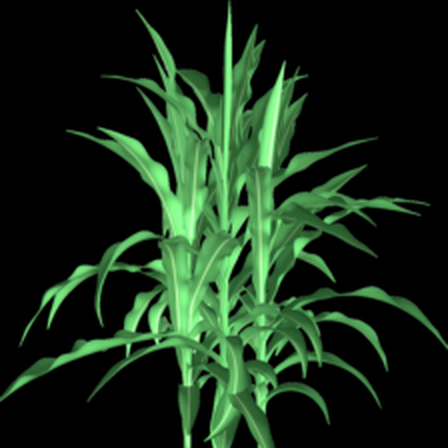
\includegraphics[width=0.9200in, height=0.9200in]{Figures/fig1/sorghum_row_photograph.png}};
\node[anchor=south west, inner sep=0] at (1.3000,1.8600) {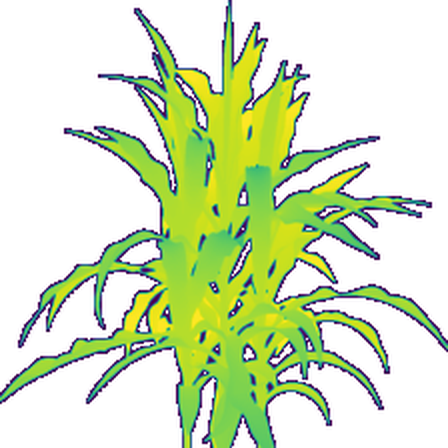
\includegraphics[width=0.3900in, height=0.3900in]{Figures/fig1/sorghum_depth.png}};
\node[anchor=south west, inner sep=0] at (1.3000,1.3300) {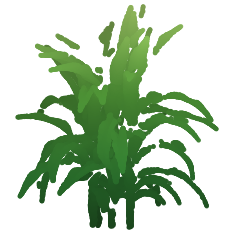
\includegraphics[width=0.3900in, height=0.3900in]{Figures/fig1/sorghum_pc.png}};
\node[anchor=south west, inner sep=0] at (3.8900,1.3300) {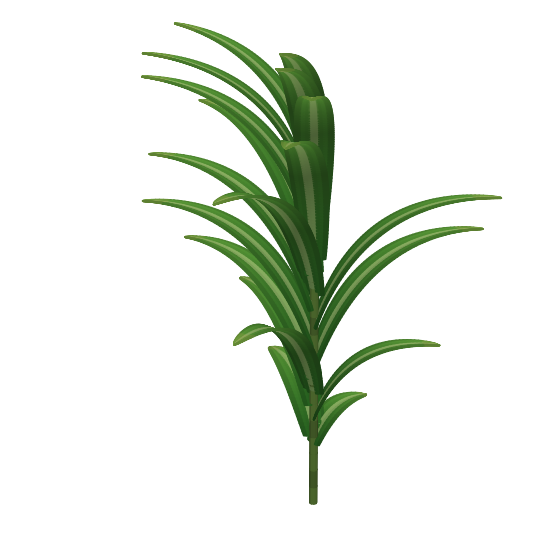
\includegraphics[width=0.9200in, height=0.9200in]{Figures/fig1/sorghum_procedural_plant.png}};
\node[anchor=south west, inner sep=0] at (0.2700,0.2600) {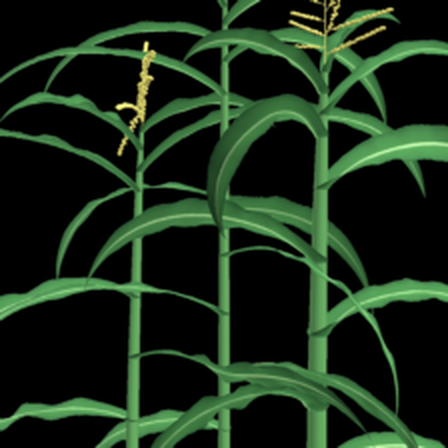
\includegraphics[width=0.9200in, height=0.9200in]{Figures/fig1/maize_row_photograph.png}};
\node[anchor=south west, inner sep=0] at (1.3000,0.7900) {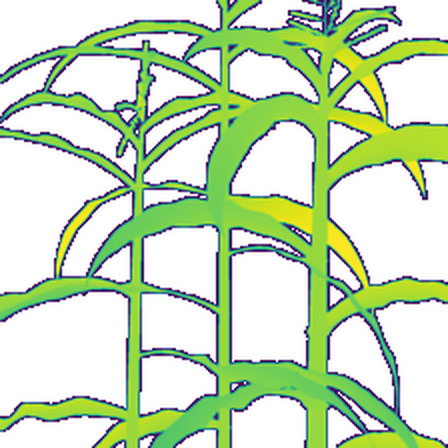
\includegraphics[width=0.3900in, height=0.3900in]{Figures/fig1/maize_depth.png}};
\node[anchor=south west, inner sep=0] at (1.3000,0.2600) {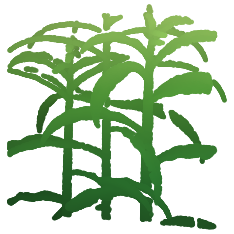
\includegraphics[width=0.3900in, height=0.3900in]{Figures/fig1/maize_pc.png}};
\node[anchor=south west, inner sep=0] at (3.8900,0.2600) {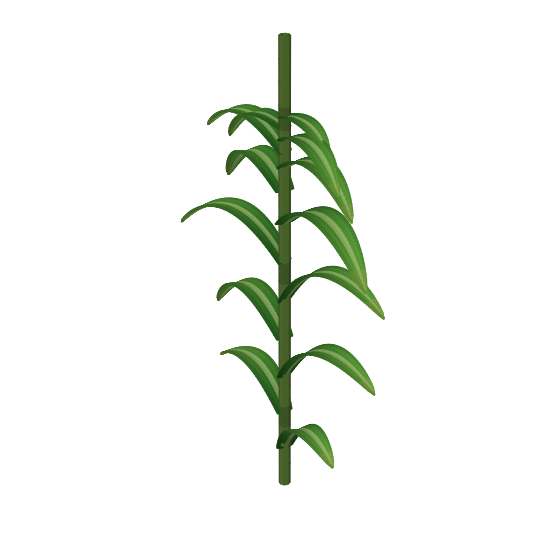
\includegraphics[width=0.9200in, height=0.9200in]{Figures/fig1/maize_procedural_plant.png}};
\draw[draw=c2B2F3A, line width=0.000pt, fill=c2B2F3A, rounded corners=0.1500in] (2.4000,1.8600) rectangle (3.3800,2.1600);
\draw[draw=cC4C6D2, line width=0.700pt, fill=cFFFFFF, rounded corners=0.0500in] (2.3700,1.2300) rectangle (3.4100,1.6100);
\draw[draw=cC4C6D2, line width=0.700pt, fill=cFFFFFF, rounded corners=0.0500in] (2.3700,0.7800) rectangle (3.4100,1.1600);
\draw[draw=cC4C6D2, line width=0.700pt, fill=cFFFFFF, rounded corners=0.0500in] (2.3700,0.3300) rectangle (3.4100,0.7100);
\draw[draw=c809EC2, line width=0.500pt, fill=c809EC2, rounded corners=0.0080in] (2.4300,1.4630) rectangle (2.4920,1.5250);
\draw[draw=c9A9AA6, line width=0.500pt, fill=cFFFFFF, rounded corners=0.0080in] (2.5040,1.4630) rectangle (2.5660,1.5250);
\draw[draw=cD091A7, line width=0.500pt, fill=cD091A7, rounded corners=0.0080in] (2.5780,1.4630) rectangle (2.6400,1.5250);
\draw[draw=c9A9AA6, line width=0.500pt, fill=cFFFFFF, rounded corners=0.0080in] (2.4300,1.3890) rectangle (2.4920,1.4510);
\draw[draw=c809EC2, line width=0.500pt, fill=c809EC2, rounded corners=0.0080in] (2.5040,1.3890) rectangle (2.5660,1.4510);
\draw[draw=c9A9AA6, line width=0.500pt, fill=cFFFFFF, rounded corners=0.0080in] (2.5780,1.3890) rectangle (2.6400,1.4510);
\draw[draw=c9A9AA6, line width=0.500pt, fill=cFFFFFF, rounded corners=0.0080in] (2.4300,1.3150) rectangle (2.4920,1.3770);
\draw[draw=c9D8CC4, line width=0.500pt, fill=c9D8CC4, rounded corners=0.0080in] (2.5040,1.3150) rectangle (2.5660,1.3770);
\draw[draw=c9A9AA6, line width=0.500pt, fill=cFFFFFF, rounded corners=0.0080in] (2.5780,1.3150) rectangle (2.6400,1.3770);
\draw[draw=cE8641C, line width=0.400pt, fill=cF28C28, line join=round] (2.6420,0.9100) -- (2.6496,0.9108) -- (2.6569,0.9131) -- (2.6636,0.9169) -- (2.6694,0.9219) -- (2.6740,0.9280) -- (2.6773,0.9349) -- (2.6792,0.9424) -- (2.6794,0.9501) -- (2.6803,0.9559) -- (2.6806,0.9618) -- (2.6804,0.9679) -- (2.6796,0.9741) -- (2.6782,0.9803) -- (2.6763,0.9868) -- (2.6738,0.9933) -- (2.6707,0.9999) -- (2.6671,1.0067) -- (2.6629,1.0136) -- (2.6582,1.0206) -- (2.6529,1.0278) -- (2.6470,1.0350) -- (2.6401,1.0266) -- (2.6338,1.0188) -- (2.6283,1.0116) -- (2.6235,1.0050) -- (2.6194,0.9989) -- (2.6161,0.9934) -- (2.6134,0.9884) -- (2.6115,0.9841) -- (2.6103,0.9803) -- (2.6098,0.9770) -- (2.6100,0.9744) -- (2.6110,0.9723) -- (2.6126,0.9708) -- (2.6095,0.9662) -- (2.6071,0.9611) -- (2.6054,0.9558) -- (2.6046,0.9502) -- (2.6046,0.9446) -- (2.6055,0.9391) -- (2.6071,0.9338) -- (2.6095,0.9287) -- (2.6127,0.9241) -- (2.6165,0.9200) -- (2.6209,0.9165) -- (2.6257,0.9137) -- (2.6310,0.9117) -- (2.6364,0.9104) -- (2.6420,0.9100) -- cycle;
\draw[draw=cF6B51E, line width=0.300pt, fill=cFFD23F, line join=round] (2.6420,0.9125) -- (2.6462,0.9129) -- (2.6502,0.9142) -- (2.6539,0.9163) -- (2.6571,0.9190) -- (2.6596,0.9224) -- (2.6614,0.9262) -- (2.6624,0.9303) -- (2.6626,0.9345) -- (2.6631,0.9377) -- (2.6632,0.9410) -- (2.6631,0.9443) -- (2.6627,0.9477) -- (2.6619,0.9512) -- (2.6609,0.9547) -- (2.6595,0.9583) -- (2.6578,0.9620) -- (2.6558,0.9657) -- (2.6535,0.9695) -- (2.6509,0.9733) -- (2.6480,0.9773) -- (2.6447,0.9813) -- (2.6409,0.9766) -- (2.6375,0.9724) -- (2.6345,0.9684) -- (2.6318,0.9647) -- (2.6296,0.9614) -- (2.6277,0.9584) -- (2.6263,0.9556) -- (2.6252,0.9532) -- (2.6246,0.9511) -- (2.6243,0.9494) -- (2.6244,0.9479) -- (2.6249,0.9468) -- (2.6258,0.9459) -- (2.6241,0.9434) -- (2.6228,0.9406) -- (2.6219,0.9377) -- (2.6214,0.9346) -- (2.6214,0.9316) -- (2.6219,0.9285) -- (2.6228,0.9256) -- (2.6241,0.9228) -- (2.6259,0.9203) -- (2.6280,0.9180) -- (2.6304,0.9161) -- (2.6331,0.9145) -- (2.6359,0.9134) -- (2.6389,0.9127) -- (2.6420,0.9125) -- cycle;
\draw[draw=c2B2F3A, line width=0.000pt, fill=c2B2F3A] (2.3700,1.5600) ellipse [x radius=0.0500, y radius=0.0500];
\draw[draw=c2B2F3A, line width=0.000pt, fill=c2B2F3A] (2.3700,1.1100) ellipse [x radius=0.0500, y radius=0.0500];
\draw[draw=c2B2F3A, line width=0.000pt, fill=c2B2F3A] (2.3700,0.6600) ellipse [x radius=0.0500, y radius=0.0500];
\draw[draw=c5B5F6B, line width=1.300pt, rounded corners=0.0800in] (2.3000,0.2300) rectangle (3.4800,2.2800);
\draw[draw=c2F7D32, line width=0.600pt, dash pattern=on 1.80pt off 1.20pt, rounded corners=0.0100in] (2.5070,0.4050) rectangle (2.5770,0.6400);
\draw[draw=cFFFFFF, line width=0.700pt, dash pattern=on 2.10pt off 1.40pt, rounded corners=0.0100in] (0.4233,1.3485) rectangle (0.9828,2.2500);
\draw[draw=cFFFFFF, line width=0.700pt, dash pattern=on 2.10pt off 1.40pt, rounded corners=0.0100in] (0.2700,0.2600) rectangle (1.1562,1.1800);
\node[anchor=west, inner sep=0, outer sep=0, align=left, text=c3F5F8F, font={\fontsize{8.50}{10.62}\selectfont\sffamily\bfseries}] at (0.2400,2.4000) {INPUT};
\node[anchor=west, inner sep=0, outer sep=0, align=left, text=c5F5F5F, font={\fontsize{8.50}{10.62}\selectfont\sffamily}] at (0.7400,2.4000) {any subset, from an occluded row};
\node[anchor=west, inner sep=0, outer sep=0, align=left, text=c5E4A96, font={\fontsize{8.50}{10.62}\selectfont\sffamily\bfseries}] at (3.8600,2.4000) {OUTPUT};
\node[anchor=west, inner sep=0, outer sep=0, align=left, text=c5F5F5F, font={\fontsize{8.50}{10.62}\selectfont\sffamily}] at (4.5800,2.4000) {procedural plant};
\node[anchor=center, inner sep=0, outer sep=0, align=center, text=cFFFFFF, font={\fontsize{11.00}{13.75}\selectfont\sffamily\bfseries}] at (2.8900,2.0100) {CropCode};
\node[anchor=center, inner sep=0, outer sep=0, align=center, text=c5F5F5F, font={\fontsize{7.50}{9.38}\selectfont\sffamily}] at (2.8900,1.7300) {one model};
\node[anchor=west, inner sep=0, outer sep=0, align=left, text=c1A1A1A, font={\fontsize{7.50}{7.88}\selectfont\sffamily}] at (2.7500,1.4200) {masked\\pretraining};
\node[anchor=center, inner sep=0, outer sep=0, align=center, text=cFFFFFF, font={\fontsize{6.50}{8.12}\selectfont\sffamily\bfseries}] at (2.3700,1.5600) {1};
\draw[draw=c2F8FD8, line width=0.900pt] (2.4850,0.9150) -- (2.4850,1.0250);
\draw[draw=c2F8FD8, line width=0.800pt] (2.4850,1.0041) -- (2.4716,1.0201);
\draw[draw=c2F8FD8, line width=0.800pt] (2.4850,1.0041) -- (2.4984,1.0201);
\draw[draw=c2F8FD8, line width=0.800pt] (2.4850,0.9359) -- (2.4984,0.9199);
\draw[draw=c2F8FD8, line width=0.800pt] (2.4850,0.9359) -- (2.4716,0.9199);
\draw[draw=c2F8FD8, line width=0.900pt] (2.4374,0.9425) -- (2.5326,0.9975);
\draw[draw=c2F8FD8, line width=0.800pt] (2.5145,0.9871) -- (2.5217,1.0067);
\draw[draw=c2F8FD8, line width=0.800pt] (2.5145,0.9871) -- (2.5351,0.9834);
\draw[draw=c2F8FD8, line width=0.800pt] (2.4555,0.9530) -- (2.4483,0.9333);
\draw[draw=c2F8FD8, line width=0.800pt] (2.4555,0.9530) -- (2.4349,0.9566);
\draw[draw=c2F8FD8, line width=0.900pt] (2.5326,0.9425) -- (2.4374,0.9975);
\draw[draw=c2F8FD8, line width=0.800pt] (2.4555,0.9871) -- (2.4349,0.9834);
\draw[draw=c2F8FD8, line width=0.800pt] (2.4555,0.9871) -- (2.4483,1.0067);
\draw[draw=c2F8FD8, line width=0.800pt] (2.5145,0.9530) -- (2.5351,0.9566);
\draw[draw=c2F8FD8, line width=0.800pt] (2.5145,0.9530) -- (2.5217,0.9333);
\draw[draw=c5B5F6B, line width=1.000pt, -{Triangle[length=2.00pt,width=2.00pt]}] (2.5500,0.9700) -- (2.5850,0.9700);
\node[anchor=west, inner sep=0, outer sep=0, align=left, text=c1A1A1A, font={\fontsize{7.50}{7.88}\selectfont\sffamily}] at (2.7500,0.9700) {cross-modal\\distillation};
\node[anchor=center, inner sep=0, outer sep=0, align=center, text=cFFFFFF, font={\fontsize{6.50}{8.12}\selectfont\sffamily\bfseries}] at (2.3700,1.1100) {2};
\draw[draw=cB4B4B4, line width=1.000pt] (2.4650,0.4200) -- (2.4650,0.6200);
\draw[draw=cB4B4B4, line width=0.900pt] (2.4650,0.4750) .. controls (2.4868,0.4821) and (2.4982,0.4971) .. (2.4990,0.5200);
\draw[draw=cB4B4B4, line width=0.900pt] (2.4650,0.5150) .. controls (2.4432,0.5221) and (2.4318,0.5371) .. (2.4310,0.5600);
\draw[draw=cB4B4B4, line width=0.900pt] (2.4650,0.5550) .. controls (2.4868,0.5621) and (2.4982,0.5771) .. (2.4990,0.6000);
\draw[draw=c2F7D32, line width=1.000pt] (2.5420,0.4200) -- (2.5420,0.6200);
\draw[draw=c2F7D32, line width=0.900pt] (2.5420,0.4750) .. controls (2.5638,0.4821) and (2.5752,0.4971) .. (2.5760,0.5200);
\draw[draw=c2F7D32, line width=0.900pt] (2.5420,0.5150) .. controls (2.5202,0.5221) and (2.5088,0.5371) .. (2.5080,0.5600);
\draw[draw=c2F7D32, line width=0.900pt] (2.5420,0.5550) .. controls (2.5638,0.5621) and (2.5752,0.5771) .. (2.5760,0.6000);
\draw[draw=cB4B4B4, line width=1.000pt] (2.6190,0.4200) -- (2.6190,0.6200);
\draw[draw=cB4B4B4, line width=0.900pt] (2.6190,0.4750) .. controls (2.6408,0.4821) and (2.6522,0.4971) .. (2.6530,0.5200);
\draw[draw=cB4B4B4, line width=0.900pt] (2.6190,0.5150) .. controls (2.5972,0.5221) and (2.5858,0.5371) .. (2.5850,0.5600);
\draw[draw=cB4B4B4, line width=0.900pt] (2.6190,0.5550) .. controls (2.6408,0.5621) and (2.6522,0.5771) .. (2.6530,0.6000);
\node[anchor=west, inner sep=0, outer sep=0, align=left, text=c1A1A1A, font={\fontsize{7.50}{7.88}\selectfont\sffamily}] at (2.7500,0.5200) {row\\fine-tuning};
\node[anchor=center, inner sep=0, outer sep=0, align=center, text=cFFFFFF, font={\fontsize{6.50}{8.12}\selectfont\sffamily\bfseries}] at (2.3700,0.6600) {3};
\node[anchor=center, inner sep=0, outer sep=0, align=center, text=c1A1A1A, font={\fontsize{8.50}{10.62}\selectfont\sffamily\bfseries}, rotate=90] at (0.1000,1.7900) {Sorghum};
\node[anchor=south west, inner sep=0, outer sep=0, align=left, text=cFFFFFF, font={\fontsize{7.00}{8.75}\selectfont\sffamily}] at (0.3100,1.3800) {27 \% hidden};
\node[anchor=north west, inner sep=0, outer sep=0, align=left, text=cA07800, font={\fontsize{7.00}{8.75}\selectfont\sffamily}] at (1.7700,2.2600) {depth};
\node[anchor=south west, inner sep=0, outer sep=0, align=left, text=cA8456E, font={\fontsize{7.00}{8.75}\selectfont\sffamily}] at (1.7700,1.3200) {cloud};
\draw[draw=c809EC2, line width=1.800pt, -{Triangle[length=3.20pt,width=3.20pt]}] (1.2300,1.7900) -- (2.2800,1.7900);
\draw[draw=cE0B020, line width=1.800pt, -{Triangle[length=3.20pt,width=3.20pt]}] (1.7400,2.0550) .. controls (1.9092,1.9433) and (2.0892,1.9217) .. (2.2800,1.9900);
\draw[draw=cD091A7, line width=1.800pt, -{Triangle[length=3.20pt,width=3.20pt]}] (1.7400,1.5250) .. controls (1.9092,1.6367) and (2.0892,1.6583) .. (2.2800,1.5900);
\node[anchor=west, inner sep=0, outer sep=0, align=left, text=c5E4A96, font={\fontsize{8.50}{10.62}\selectfont\sffamily\bfseries}] at (4.9400,2.1000) {written by CropCode};
\node[anchor=west, inner sep=0, outer sep=0, align=left, text=c5F5F5F, font={\fontsize{8.50}{10.62}\selectfont\sffamily\bfseries}] at (6.3200,2.1000) {true};
\node[anchor=west, inner sep=0, outer sep=0, align=left, text=c5F5F5F, font={\fontsize{8.50}{10.62}\selectfont\sffamily}] at (4.9400,1.8600) {height};
\node[anchor=west, inner sep=0, outer sep=0, align=left, text=c5E4A96, font={\fontsize{8.50}{10.62}\selectfont\sffamily\bfseries}] at (5.7400,1.8600) {0.93 m};
\node[anchor=west, inner sep=0, outer sep=0, align=left, text=c5F5F5F, font={\fontsize{8.50}{10.62}\selectfont\sffamily}] at (6.3200,1.8600) {0.94 m};
\node[anchor=west, inner sep=0, outer sep=0, align=left, text=c5F5F5F, font={\fontsize{8.50}{10.62}\selectfont\sffamily}] at (4.9400,1.6700) {leaves};
\node[anchor=west, inner sep=0, outer sep=0, align=left, text=c5E4A96, font={\fontsize{8.50}{10.62}\selectfont\sffamily\bfseries}] at (5.7400,1.6700) {19};
\node[anchor=west, inner sep=0, outer sep=0, align=left, text=c5F5F5F, font={\fontsize{8.50}{10.62}\selectfont\sffamily}] at (6.3200,1.6700) {19};
\node[anchor=west, inner sep=0, outer sep=0, align=left, text=c5F5F5F, font={\fontsize{8.50}{10.62}\selectfont\sffamily}] at (4.9400,1.4800) {leaf length};
\node[anchor=west, inner sep=0, outer sep=0, align=left, text=c5E4A96, font={\fontsize{8.50}{10.62}\selectfont\sffamily\bfseries}] at (5.7400,1.4800) {0.74 m};
\node[anchor=west, inner sep=0, outer sep=0, align=left, text=c5F5F5F, font={\fontsize{8.50}{10.62}\selectfont\sffamily}] at (6.3200,1.4800) {0.76 m};
\draw[draw=c9D8CC4, line width=1.800pt, -{Triangle[length=3.20pt,width=3.20pt]}] (3.5000,1.7900) -- (3.8400,1.7900);
\node[anchor=center, inner sep=0, outer sep=0, align=center, text=c1A1A1A, font={\fontsize{8.50}{10.62}\selectfont\sffamily\bfseries}, rotate=90] at (0.1000,0.7200) {Maize};
\node[anchor=south west, inner sep=0, outer sep=0, align=left, text=cFFFFFF, font={\fontsize{7.00}{8.75}\selectfont\sffamily}] at (0.3100,0.3100) {22 \% hidden};
\node[anchor=north west, inner sep=0, outer sep=0, align=left, text=cA07800, font={\fontsize{7.00}{8.75}\selectfont\sffamily}] at (1.7700,1.1900) {depth};
\node[anchor=south west, inner sep=0, outer sep=0, align=left, text=cA8456E, font={\fontsize{7.00}{8.75}\selectfont\sffamily}] at (1.7700,0.2500) {cloud};
\draw[draw=c809EC2, line width=1.800pt, -{Triangle[length=3.20pt,width=3.20pt]}] (1.2300,0.7200) -- (2.2800,0.7200);
\draw[draw=cE0B020, line width=1.800pt, -{Triangle[length=3.20pt,width=3.20pt]}] (1.7400,0.9850) .. controls (1.9092,0.8733) and (2.0892,0.8517) .. (2.2800,0.9200);
\draw[draw=cD091A7, line width=1.800pt, -{Triangle[length=3.20pt,width=3.20pt]}] (1.7400,0.4550) .. controls (1.9092,0.5667) and (2.0892,0.5883) .. (2.2800,0.5200);
\node[anchor=west, inner sep=0, outer sep=0, align=left, text=c5E4A96, font={\fontsize{8.50}{10.62}\selectfont\sffamily\bfseries}] at (4.9400,1.0300) {written by CropCode};
\node[anchor=west, inner sep=0, outer sep=0, align=left, text=c5F5F5F, font={\fontsize{8.50}{10.62}\selectfont\sffamily\bfseries}] at (6.3200,1.0300) {true};
\node[anchor=west, inner sep=0, outer sep=0, align=left, text=c5F5F5F, font={\fontsize{8.50}{10.62}\selectfont\sffamily}] at (4.9400,0.7900) {height};
\node[anchor=west, inner sep=0, outer sep=0, align=left, text=c5E4A96, font={\fontsize{8.50}{10.62}\selectfont\sffamily\bfseries}] at (5.7400,0.7900) {1.07 m};
\node[anchor=west, inner sep=0, outer sep=0, align=left, text=c5F5F5F, font={\fontsize{8.50}{10.62}\selectfont\sffamily}] at (6.3200,0.7900) {1.06 m};
\node[anchor=west, inner sep=0, outer sep=0, align=left, text=c5F5F5F, font={\fontsize{8.50}{10.62}\selectfont\sffamily}] at (4.9400,0.6000) {leaves};
\node[anchor=west, inner sep=0, outer sep=0, align=left, text=c5E4A96, font={\fontsize{8.50}{10.62}\selectfont\sffamily\bfseries}] at (5.7400,0.6000) {13};
\node[anchor=west, inner sep=0, outer sep=0, align=left, text=c5F5F5F, font={\fontsize{8.50}{10.62}\selectfont\sffamily}] at (6.3200,0.6000) {13};
\node[anchor=west, inner sep=0, outer sep=0, align=left, text=c5F5F5F, font={\fontsize{8.50}{10.62}\selectfont\sffamily}] at (4.9400,0.4100) {leaf length};
\node[anchor=west, inner sep=0, outer sep=0, align=left, text=c5E4A96, font={\fontsize{8.50}{10.62}\selectfont\sffamily\bfseries}] at (5.7400,0.4100) {0.36 m};
\node[anchor=west, inner sep=0, outer sep=0, align=left, text=c5F5F5F, font={\fontsize{8.50}{10.62}\selectfont\sffamily}] at (6.3200,0.4100) {0.37 m};
\draw[draw=c9D8CC4, line width=1.800pt, -{Triangle[length=3.20pt,width=3.20pt]}] (3.5000,0.7200) -- (3.8400,0.7200);
\node[anchor=west, inner sep=0, outer sep=0, align=left, text=c5F5F5F, font={\fontsize{7.00}{8.75}\selectfont\sffamily}] at (0.2400,0.0700) {no mask or bounding box given  ·  here: all three streams (any subset is accepted)};
\node[anchor=east, inner sep=0, outer sep=0, align=right, text=c5E4A96, font={\fontsize{7.50}{9.38}\selectfont\sffamily}] at (6.8350,0.0700) {kilobytes  ·  editable  ·  re-renderable};
\end{tikzpicture}%
}%
}%
    \vspace{-20pt}
    \caption{\textbf{Input: any modality; Output: procedural plant.}
    Given any modality (RGB, depth, or point cloud) from occluded crop rows, \method{} predicts procedural parameters that re-render into a complete 3D plant. Shown are held-out simulated rows of two species; dashed boxes mark target plants but are not provided to the model. Using all three input streams, the row-fine-tuned model predicts the target's procedural parameters, which are then used to render a textured 3D plant. Predicted heights are within 1\% of ground truth, and leaf counts match exactly for both plants.}
    \label{fig:teaser}%
\end{center}%
\vspace{4.0pt}
}]


%%%%%%%%%%%%%%%%%%%%%%%%%%%%%%%%%%%%%%%%%%%%%%%%%%%%%%%%%%%%%%%%%%%%%%%%%%%
% ABSTRACT
%%%%%%%%%%%%%%%%%%%%%%%%%%%%%%%%%%%%%%%%%%%%%%%%%%%%%%%%%%%%%%%%%%%%%%%%%%%
\begin{abstract}

Recovering thin, heavily occluded structures from sparse sensing remains an open problem in 3D vision. In agriculture, row crops are an extreme case of this problem. Leaves are millimeters thick and up to a meter long, and neighboring plants in a row occlude one another. Routine field imaging campaigns capture only a single photograph, a noisy depth map, or a partial point cloud per plant. We introduce \method{}, which recovers the complete procedural model of a plant from any subset of RGB, depth, and point-cloud observations in a single forward pass. The procedural model (the generator parameters for leaf count, insertion heights, leaf angles, and surface geometry) is compact, interpretable, and auditable. We use a realistic plant procedural generator as both the training data and the output space. We pretrain a masked autoencoder on all modalities of 15{,}000 generated plants per species (maize and sorghum) and specialize it in two ways: we distill it into single-sensor students, and we fine-tune it on agronomically realistic simulated crop rows in which neighboring leaves bend and deform upon contact. Fine-tuning on simulated rows removes 85\% (sorghum) and 92\% (maize) of the reconstruction error introduced by occluding neighbors. On rendered rows assembled from real plants, zero-shot predictions degrade for plants taller than the synthetic training range, but fine-tuning on real plants reduces the median height error on held-out maize plants to 1.6\%, with an inference time of milliseconds per plant. From a single image of an isolated plant, \method{} reconstructs the 3D plant and predicts leaf count within one leaf on 91\% (sorghum) and 97\% (maize) of plants. In contrast, a two-stage variant of our model that first generates a point cloud from the image and then infers the parameters from that cloud reaches only 30\% (sorghum) and 7\% (maize). Training on all modalities improves single-sensor predictions, and distillation reduces the cross-modal generation loss by 30\% in sorghum and 44\% in maize. We also release \dataset{}, a 30{,}000-plant, two-species benchmark that pairs RGB, depth, and point-cloud captures under simulated row occlusion with exact procedural ground truth. \method{} is a step toward generating plant-level 3D digital assets at field scale for agriculture. Code and project page: \href{https://anonymous.4open.science/w/CropCode/}{Crop Code}.
\end{abstract}
% REVIEWER FLAG (V3): abstract sentences are the author's, reordered so that the row-occlusion and real-plant results come first. Three phrases changed: 'specialize it in two ways', 'two-stage variant of our model ... predicts the parameters from it' (was 'baseline ... fits'), and 'rendered rows assembled from real plants' (was '(from the field)').


%%%%%%%%%%%%%%%%%%%%%%%%%%%%%%%%%%%%%%%%%%%%%%%%%%%%%%%%%%%%%%%%%%%%%%%%%%%
% 1. INTRODUCTION
%%%%%%%%%%%%%%%%%%%%%%%%%%%%%%%%%%%%%%%%%%%%%%%%%%%%%%%%%%%%%%%%%%%%%%%%%%%
\section{Introduction}
\label{sec:intro}

Recovering the 3D structure of thin, heavily occluded objects from sparse sensing remains an open problem in computer vision. The problem is becoming more pressing. Autonomous ground robots now make routine measurements in crop fields and forests~\citep{kayacan2018terrasentia,muellersim2017robotanist,xu2022groundrobots,mattamala2024forest}, and they view plants from within the canopy, in a single pass, where the plants are heavily occluded by their neighbors. Row crops are an extreme case of this problem. A maize leaf is only centimeters wide and millimeters thick, yet up to a meter long, and it is tightly interleaved with the leaves of neighboring plants in the row. In our simulated maize rows, neighboring plants account for 59 to 68\% of the plant pixels. The problem is also of practical importance. Accurate 3D models of individual plants are increasingly used by breeders and agronomists to measure morphological traits (such as leaf angle, internode length, and canopy structure) at scale, and they are required for agricultural digital twins and for the \emph{in silico} evaluation of crop ideotypes~\citep{pylianidis2021digitaltwins,verdouw2021digitaltwins,soualiou2021fspm,hadadi2025procmaize, maizefield3d2025}. The global precision farming market is estimated at \$12.8 billion in 2025~\citep{bcc2025precisionfarming}, and the commercial seed market, which depends on row-crop breeding, adds more than \$50 billion per year~\citep{mordor2026seed}.


Standard 3D completion methods, however, are designed for compact, mostly convex objects~\citep{yuan2018pcn,yu2021pointr}, and the Chamfer distance used to train and score them is insensitive to thin sheets~\citep{wu2021dcd, song2026structural}. Recent occlusion-aware plant completion methods recover the missing geometry, but their output is an unstructured point cloud~\citep{lee2026occ}, which still has to be analyzed to recover the plant traits. We find that this second step is fragile. A two-stage variant of our model that generates a point cloud from an image and then infers the plant parameters from that cloud predicts leaf count within one leaf on only 30\% of sorghum plants and 7\% of maize plants (see \secref{sec:regime1}).


We instead predict a procedural model of the plant directly. A procedural model is a textual description that represents a plant as a compact set of biologically meaningful parameters, which are expanded by a generator into complete, editable, simulation-ready 3D geometry~\citep{prusin1990abop, floraforge2026}. This representation has several advantages. First, it is compact (a few kilobytes instead of megabytes). It is also interpretable, explainable, human-readable, and auditable, since the parameters are biologically relevant traits that can be checked against measurements. Finally, prior information, such as the growth stage or the planting density, can be supplied as known parameters alongside the sensor data (\secref{sec:exp-main}). However, existing methods for recovering procedural plant models rely on \textit{clean, high-density observations} of isolated plants~\citep{cropcraft2026,demeter2025, ghrer2025paramplants}. The most accurate pipeline requires a complete terrestrial laser scan of an isolated plant and roughly ten minutes of processing per plant~\citep{hadadi2026vlmmaize}. To our knowledge, prior methods do not recover a complete, re-renderable procedural plant from a single observation under row-neighbor occlusion.

In this work, we introduce \method{} (\figref{fig:arch}). We use a realistic plant procedural generator as both the training data  and the output space. We pretrain a four-modality masked autoencoder~\citep{he2022mae,bachmann2022multimae,mizrahi2023fourm,dong2025embodiedmae} over RGB images, depth maps, point clouds, and tokenized procedural parameters on 15{,}000 generated plants per species (maize and sorghum). We mask random subsets of tokens across the modalities during pretraining. This random masking allows a single network to infer the missing streams from any available sensor combination. We then specialize the pretrained model in two ways. For single-sensor inference, we distill the model~\citep{hinton2015distillation} into single-sensor students. For plants in crop rows, we fine-tune the model on simulated rows whose neighboring leaves bend on contact. At inference, the input is any available subset of the sensor streams, and the output is the procedural plant.

Training \method{} requires data that pairs \textit{field-like sensing with exact procedural ground truth}. We therefore build \dataset{}, a 30{,}000-plant, two-species dataset with four aligned streams per view (RGB, depth, point cloud, and procedural parameters). It includes simulated crop rows in which an articulated contact solver bends neighboring leaves around one another, and \textit{rows assembled from real plants} (\tabref{tab:datacompare}). The realism of the occlusion matters. Training on contact-solved rows gives a row reconstruction $F_1$ of 0.789, compared with 0.717 for unbent neighbors and 0.416 for isolated plants (\secref{sec:regime3}). Our main contributions are:
\begin{enumerate}
  \item \textbf{Task and method.} We introduce the first amortized method that recovers complete, editable procedural plant models of slender, row-occluded crops from \emph{any subset} of RGB, depth, and point-cloud inputs in a single forward pass. It consists of a multimodal pretraining stage and two specializations (single-sensor distillation and row-occlusion fine-tuning).
  \item \textbf{The \dataset{} benchmark.} We release \dataset{}, including an evaluation split built from real plants of diverse maize and sorghum varieties.
  \item \textbf{Reconstruction under row occlusion.} A model trained using only isolated plants performs poorly on row crops with occlusion. Fine-tuning on simulated rows, without bounding boxes or masks, restores most of the lost accuracy.
  \item \textbf{Transfer to real plants.} On rows assembled from real maize and sorghum plants~\citep{maizefield3d2025}, fine-tuning on 75\% of the plants reduces the median height error on held-out maize plants to 1.6\%, and the fine-tuned model predicts leaf count within one leaf on 70\% of captures. Inference also takes only milliseconds per plant.
\end{enumerate}
% REVIEWER FLAG: contributions changed from the earlier draft. The parameter-visibility design rule and the Chamfer-vs-probe protocol are no longer listed as contributions (both analyses are in Appendix app:analyses).

%%%%%%%%%%%%%%%%%%%%%%%%%%%%%%%%%%%%%%%%%%%%%%%%%%%%%%%%%%%%%%%%%%%%%%%%%%%
% 2. RELATED WORK
%%%%%%%%%%%%%%%%%%%%%%%%%%%%%%%%%%%%%%%%%%%%%%%%%%%%%%%%%%%%%%%%%%%%%%%%%%%
\section{Related Work}
\label{sec:related}

\noindent\textbf{Recovering procedural plant models.}
Classical methods for inverse procedural modeling estimate tree generator parameters per instance, using stochastic optimization~\citep{stava2014ipmtrees}, MCMC sampling~\citep{talton2011metropolis}, or L-system induction~\citep{guo2020ipmlsys,latentlsys2023}. Recent learned methods use diffusion priors to reconstruct 3D trees from a single image~\citep{svdtree2024,lee2024treedfusion}. Recent crop-focused methods infer parametric morphology from clean, complete 3D point clouds~\citep{demeter2025,ghrer2025paramplants}, optimize procedural parameters against multi-view NeRF reconstructions~\citep{cropcraft2026}, or combine vision-language prompting with differentiable NURBS fitting on terrestrial laser scans~\citep{hadadi2026vlmmaize,nurbsdiff2022}. Specifying the procedural parameters manually, by comparison, takes hours per plant~\citep{floraforge2026}. These automated methods, however, assume a clean observation of an isolated plant or require minutes of per-plant optimization. \textit{They do not apply to our setting, in which a plant occluded by its row neighbors is observed from a single view.}


\noindent\textbf{Inferring programs from visual observations.}
Outside of agriculture, feed-forward models have been trained to infer 3D shape programs~\citep{shapeprograms2019}, procedural generator parameters~\citep{zhao2025dipcg}, and executable CAD command sequences~\citep{text2cad2024,kolodiazhnyi2025cadrille} from images or point clouds. These models target rigid, isolated man-made objects under clean viewing conditions, without inter-object occlusion or deformable thin organs, both of which are present in crop rows.

\noindent\textbf{Point-cloud completion and slender geometry.}
Deep point-cloud completion networks~\citep{yuan2018pcn,yu2021pointr,yu2023adapointr,cai2024einet}, which predict the missing geometry of a partial point cloud, are primarily developed on compact, mostly convex shapes. Recent methods for occluded plant completion~\citep{lee2026occ} and thin-structure reconstruction~\citep{curvegaussian2025,qi2026rethinking} handle slender geometry. However, these methods output unstructured point clouds, which are not editable, trait-level procedural models. In addition, the standard Chamfer distance used to train and score completion networks is insensitive to thin surfaces~\citep{wu2021dcd,song2026structural,lin2023infocd}. We address this insensitivity by training with a distribution-matching loss and by scoring the predicted procedural parameters (\secref{sec:exp-setup}).

\noindent\textbf{Multimodal masked pretraining and synthetic data.}
Masked autoencoding~\citep{he2022mae} has been extended to multimodal images~\citep{bachmann2022multimae}, any-to-any generation~\citep{mizrahi2023fourm,bachmann2024fourm21}, 3D point clouds~\citep{pang2022pointmae}, and joint RGB, depth, and point-cloud inputs in EmbodiedMAE~\citep{dong2025embodiedmae}, which is the backbone of \method{}. We introduce a fourth structured modality, namely continuous procedural parameters embedded via xVal-style numerical tokens~\citep{golkar2023xval}. We also distill a full-modality teacher~\citep{hinton2015distillation} into single-sensor students to handle missing modalities at test time~\citep{wang2024robustmissing}. Pretraining on procedural synthetic data is well established~\citep{kataoka2020fractaldb,raistrick2023infinigen,greff2022kubric,tobin2017domainrand,fan2023intriguing}. In our setting, the procedural plant generator produces the training data and also defines the exact output space. Please refer to the Appendix for an expanded literature survey.
% APPENDIX REF (removed for submission, restore later): \appendixref{app:litreview} (was: \appendixref{app:litreview} gives an expanded survey.)


\begin{figure*}[t]
  \centering
  \resizebox{\linewidth}{!}{% PROCEDURAL 2026-11-13: Stage 2/3 before/after tiles show the written procedural model (true recipe grey
% underneath), from figures/make_fig2_recipe_tiles.py, with parameter MAE instead of Chamfer.
% LAYOUT v3 2026-11-13: Inside-CropCode panel left, stages center, warm-start
% label+arcs mirrored to the far RIGHT edge.
% LAYOUT SWAP 2026-11-13 (user request): Inside-CropCode panel moved to the LEFT,
% the three stages (and warm-start arrows) to the RIGHT. Applied as a coordinate
% transform on the generated file: x>=5.04 -> x-5.08, else x+1.895. Re-running
% figures/_scene.py would regenerate the ORIGINAL layout and undo this.
% Generated by figures/_scene.py (Scene.render_tikz) for 'Fig 2 stages'; do not edit by hand, re-run the figure script.
% 6.875 x 4.42 in at 100 %; needs \usetikzlibrary{arrows.meta}; images in Figures/fig2/.
{%
\definecolor{c1D221C}{HTML}{1D221C}%
\definecolor{c2A9D8F}{HTML}{2A9D8F}%
\definecolor{c2B3A67}{HTML}{2B3A67}%
\definecolor{c30638E}{HTML}{30638E}%
\definecolor{c4A78B5}{HTML}{4A78B5}%
\definecolor{c5F685C}{HTML}{5F685C}%
\definecolor{c6AA84F}{HTML}{6AA84F}%
\definecolor{c888888}{HTML}{888888}%
\definecolor{c8A8A8A}{HTML}{8A8A8A}%
\definecolor{cB8860B}{HTML}{B8860B}%
\definecolor{cC0392B}{HTML}{C0392B}%
\definecolor{cD9E2F3}{HTML}{D9E2F3}%
\definecolor{cE0A82E}{HTML}{E0A82E}%
\definecolor{cEEF3FA}{HTML}{EEF3FA}%
\definecolor{cF1F8EE}{HTML}{F1F8EE}%
\definecolor{cF4F4F2}{HTML}{F4F4F2}%
\definecolor{cFBE3C4}{HTML}{FBE3C4}%
\definecolor{cFDF8EA}{HTML}{FDF8EA}%
\definecolor{cFFFFFF}{HTML}{FFFFFF}%
\begin{tikzpicture}[x=1in, y=1in]%
\useasboundingbox (0,0) rectangle (6.8750,4.4200);
\draw[draw=cE0A82E, line width=1.200pt, fill=cFDF8EA, rounded corners=0.0900in] (1.9150,2.7200) rectangle (6.4950,4.2800);
\draw[draw=cE0A82E, line width=0.900pt, fill=cFFFFFF, rounded corners=0.0500in] (2.0550,4.1700) rectangle (3.9008,4.3900);
\draw[draw=c6AA84F, line width=1.200pt, fill=cF1F8EE, rounded corners=0.0900in] (1.9150,1.4000) rectangle (6.4950,2.5600);
\draw[draw=c6AA84F, line width=0.900pt, fill=cFFFFFF, rounded corners=0.0500in] (2.0550,2.4500) rectangle (4.1513,2.6700);
\draw[draw=c4A78B5, line width=1.200pt, fill=cEEF3FA, rounded corners=0.0900in] (1.9150,0.0400) rectangle (6.4950,1.2400);
\draw[draw=c4A78B5, line width=0.900pt, fill=cFFFFFF, rounded corners=0.0500in] (2.0550,1.1300) rectangle (3.7600,1.3500);
\draw[draw=c2B3A67, line width=0.900pt, fill=cD9E2F3, line join=round] (4.1350,3.0300) -- (4.8073,3.2292) -- (4.8073,3.6608) -- (4.1350,3.8600) -- cycle;
\draw[draw=c2B3A67, line width=0.900pt, fill=cFBE3C4, line join=round] (4.8423,3.2458) -- (5.4150,3.1130) -- (5.4150,3.7770) -- (4.8423,3.6442) -- cycle;
\draw[draw=c888888, line width=0.900pt, fill=cFFFFFF, rounded corners=0.0500in] (2.0350,1.5500) rectangle (3.2850,2.2700);
\draw[draw=c2B3A67, line width=1.000pt, fill=cFFFFFF, rounded corners=0.0500in] (3.8150,1.5500) rectangle (5.0650,2.2700);
\draw[draw=c2B3A67, line width=0.900pt, fill=cD9E2F3, line join=round] (3.7450,0.4200) -- (4.3741,0.5256) -- (4.3741,0.7544) -- (3.7450,0.8600) -- cycle;
\draw[draw=c2B3A67, line width=0.900pt, fill=cFBE3C4, line join=round] (4.4091,0.5344) -- (4.9450,0.4640) -- (4.9450,0.8160) -- (4.4091,0.7456) -- cycle;
\draw[draw=c8A8A8A, line width=1.300pt, fill=cF4F4F2, rounded corners=0.0900in] (0.0200,0.0400) rectangle (1.7750,4.2800);
\draw[draw=cC0392B, line width=0.600pt, fill=cC0392B, rounded corners=0.0120in] (0.1600,3.6500) rectangle (0.2800,3.7700);
\draw[draw=cC0392B, line width=0.600pt, fill=cFFFFFF, rounded corners=0.0120in] (0.3150,3.6500) rectangle (0.4350,3.7700);
\draw[draw=cC0392B, line width=0.600pt, fill=cC0392B, rounded corners=0.0120in] (0.4700,3.6500) rectangle (0.5900,3.7700);
\draw[draw=cC0392B, line width=0.600pt, fill=cFFFFFF, rounded corners=0.0120in] (0.6250,3.6500) rectangle (0.7450,3.7700);
\draw[draw=cB8860B, line width=0.600pt, fill=cFFFFFF, rounded corners=0.0120in] (0.1600,3.3500) rectangle (0.2800,3.4700);
\draw[draw=cB8860B, line width=0.600pt, fill=cB8860B, rounded corners=0.0120in] (0.3150,3.3500) rectangle (0.4350,3.4700);
\draw[draw=cB8860B, line width=0.600pt, fill=cFFFFFF, rounded corners=0.0120in] (0.4700,3.3500) rectangle (0.5900,3.4700);
\draw[draw=cB8860B, line width=0.600pt, fill=cFFFFFF, rounded corners=0.0120in] (0.6250,3.3500) rectangle (0.7450,3.4700);
\draw[draw=c2A9D8F, line width=0.600pt, fill=c2A9D8F, rounded corners=0.0120in] (0.1600,3.0500) rectangle (0.2800,3.1700);
\draw[draw=c2A9D8F, line width=0.600pt, fill=c2A9D8F, rounded corners=0.0120in] (0.3150,3.0500) rectangle (0.4350,3.1700);
\draw[draw=c2A9D8F, line width=0.600pt, fill=cFFFFFF, rounded corners=0.0120in] (0.4700,3.0500) rectangle (0.5900,3.1700);
\draw[draw=c2A9D8F, line width=0.600pt, fill=c2A9D8F, rounded corners=0.0120in] (0.6250,3.0500) rectangle (0.7450,3.1700);
\draw[draw=c30638E, line width=0.600pt, fill=c30638E, rounded corners=0.0120in] (0.1600,2.7500) rectangle (0.2800,2.8700);
\draw[draw=c30638E, line width=0.600pt, fill=cFFFFFF, rounded corners=0.0120in] (0.3150,2.7500) rectangle (0.4350,2.8700);
\draw[draw=c30638E, line width=0.600pt, fill=cFFFFFF, rounded corners=0.0120in] (0.4700,2.7500) rectangle (0.5900,2.8700);
\draw[draw=c30638E, line width=0.600pt, fill=c30638E, rounded corners=0.0120in] (0.6250,2.7500) rectangle (0.7450,2.8700);
\draw[draw=cC0392B, line width=0.300pt, fill=cC0392B, rounded corners=0.0100in] (0.1600,1.9200) rectangle (0.6073,2.0500);
\draw[draw=cB8860B, line width=0.300pt, fill=cB8860B, rounded corners=0.0100in] (0.6073,1.9200) rectangle (0.7403,2.0500);
\draw[draw=c2A9D8F, line width=0.300pt, fill=c2A9D8F, rounded corners=0.0100in] (0.7403,1.9200) rectangle (1.4174,2.0500);
\draw[draw=c30638E, line width=0.300pt, fill=c30638E, rounded corners=0.0100in] (1.4174,1.9200) rectangle (1.6350,2.0500);
\draw[draw=c2B3A67, line width=0.800pt, fill=cD9E2F3, rounded corners=0.0400in] (0.1600,1.0600) rectangle (1.6350,1.4800);
\draw[draw=c2B3A67, line width=0.800pt, fill=cFBE3C4, rounded corners=0.0400in] (0.1600,0.5000) rectangle (1.6350,0.9200);
\draw[draw=cC0392B, line width=0.500pt, fill=cC0392B, rounded corners=0.0200in] (0.1600,0.1300) rectangle (0.5062,0.2300);
\draw[draw=cB8860B, line width=0.500pt, fill=cB8860B, rounded corners=0.0200in] (0.5362,0.1300) rectangle (0.8825,0.2300);
\draw[draw=c2A9D8F, line width=0.500pt, fill=c2A9D8F, rounded corners=0.0200in] (0.9125,0.1300) rectangle (1.2588,0.2300);
\draw[draw=c30638E, line width=0.500pt, fill=c30638E, rounded corners=0.0200in] (1.2888,0.1300) rectangle (1.6350,0.2300);
\node[anchor=south west, inner sep=0] at (2.0350,3.4600) {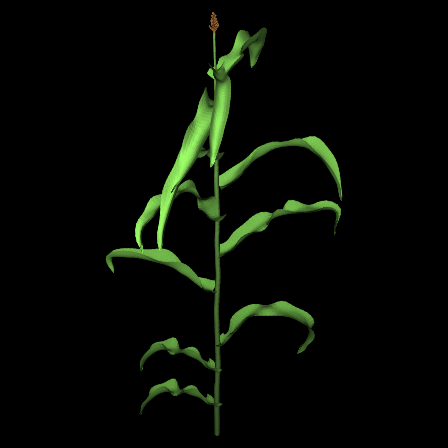
\includegraphics[width=0.4000in, height=0.4000in]{Figures/fig2/image.png}};
\node[anchor=south west, inner sep=0] at (2.4650,3.4600) {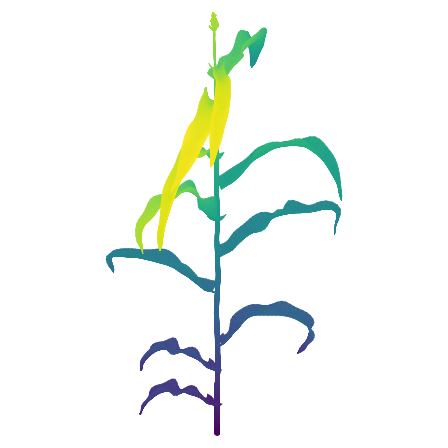
\includegraphics[width=0.4000in, height=0.4000in]{Figures/fig2/depth_image.png}};
\node[anchor=south west, inner sep=0] at (2.0350,3.0300) {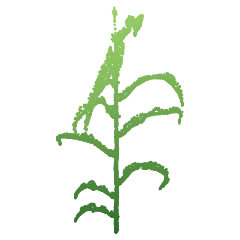
\includegraphics[width=0.4000in, height=0.4000in]{Figures/fig2/point_cloud.png}};
\node[anchor=south west, inner sep=0] at (2.4650,3.0300) {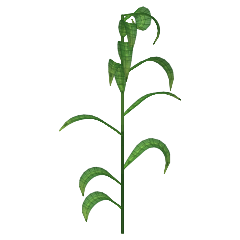
\includegraphics[width=0.4000in, height=0.4000in]{Figures/fig2/parameters.png}};
\node[anchor=south west, inner sep=0] at (3.0650,3.4600) {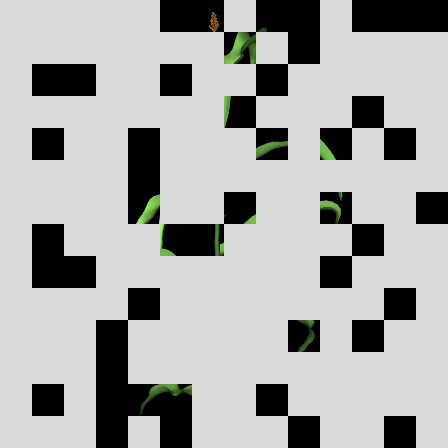
\includegraphics[width=0.4000in, height=0.4000in]{Figures/fig2/image_masked.png}};
\node[anchor=south west, inner sep=0] at (3.4950,3.4600) {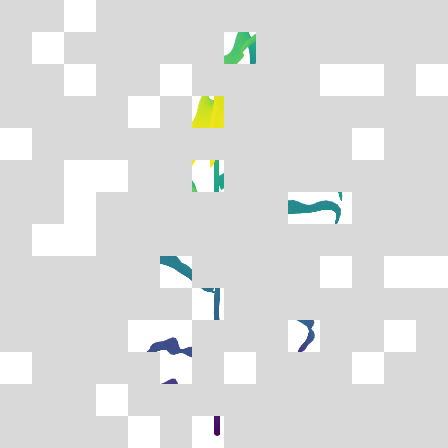
\includegraphics[width=0.4000in, height=0.4000in]{Figures/fig2/depth_masked.png}};
\node[anchor=south west, inner sep=0] at (3.0650,3.0300) {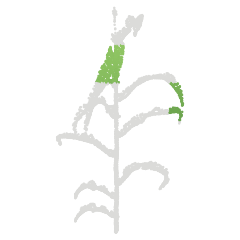
\includegraphics[width=0.4000in, height=0.4000in]{Figures/fig2/cloud_masked.png}};
\node[anchor=south west, inner sep=0] at (3.4950,3.0300) {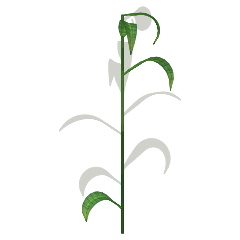
\includegraphics[width=0.4000in, height=0.4000in]{Figures/fig2/parameters_masked.png}};
\node[anchor=south west, inner sep=0] at (5.5750,3.4600) {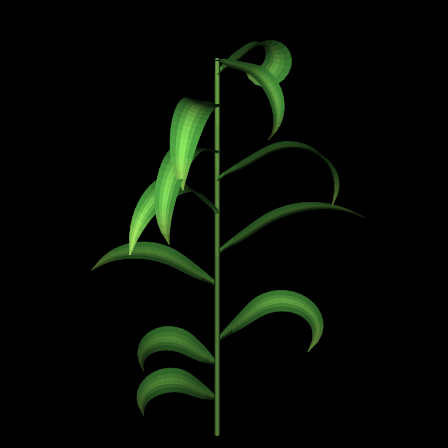
\includegraphics[width=0.4000in, height=0.4000in]{Figures/fig2/image_output.png}};
\node[anchor=south west, inner sep=0] at (6.0050,3.4600) {
\includegraphics[width=0.4000in, height=0.4000in]{Figures/fig2/depth_output.png}};
\node[anchor=south west, inner sep=0] at (5.5750,3.0300) {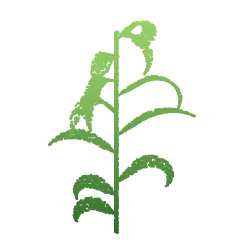
\includegraphics[width=0.4000in, height=0.4000in]{Figures/fig2/cloud_output.png}};
\node[anchor=south west, inner sep=0] at (6.0050,3.0300) {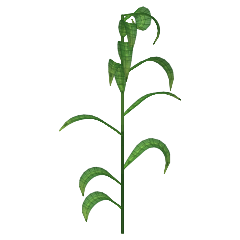
\includegraphics[width=0.4000in, height=0.4000in]{Figures/fig2/parameters_output.png}};
\node[anchor=south west, inner sep=0] at (4.7100,3.7250) {
\includegraphics[width=0.1700in, height=0.1700in]{Figures/fig2/fire.png}};
\node[anchor=south west, inner sep=0] at (2.1100,2.0250) {
\includegraphics[width=0.1700in, height=0.1700in]{Figures/fig2/snow.png}};
\node[anchor=south west, inner sep=0] at (2.0950,1.6200) {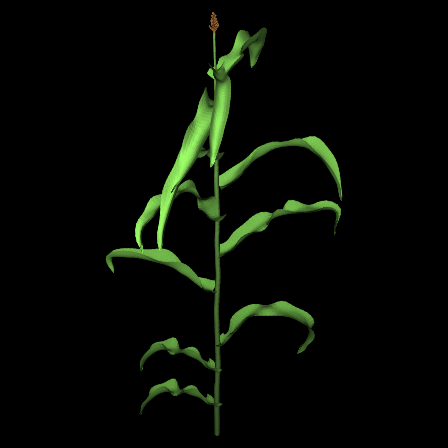
\includegraphics[width=0.2600in, height=0.2600in]{Figures/fig2/teacher_image.png}};
\node[anchor=south west, inner sep=0] at (2.3950,1.6200) {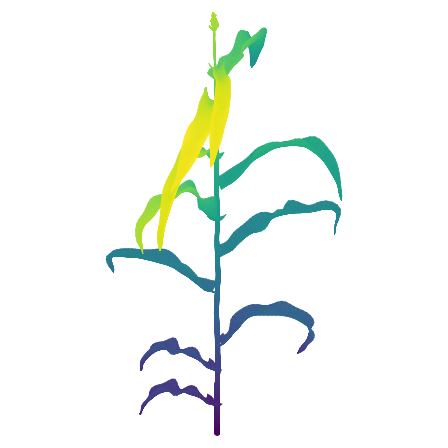
\includegraphics[width=0.2600in, height=0.2600in]{Figures/fig2/teacher_depth_image.png}};
\node[anchor=south west, inner sep=0] at (2.6950,1.6200) {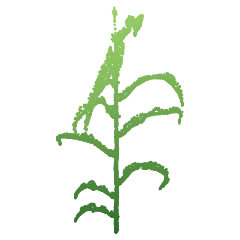
\includegraphics[width=0.2600in, height=0.2600in]{Figures/fig2/teacher_point_cloud.png}};
\node[anchor=south west, inner sep=0] at (2.9950,1.6200) {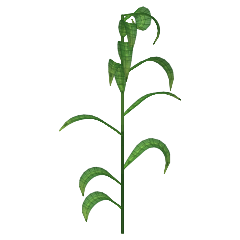
\includegraphics[width=0.2600in, height=0.2600in]{Figures/fig2/teacher_parameters.png}};
\node[anchor=south west, inner sep=0] at (3.8900,2.0250) {
\includegraphics[width=0.1700in, height=0.1700in]{Figures/fig2/fire_2.png}};
\node[anchor=south west, inner sep=0] at (3.8750,1.6200) {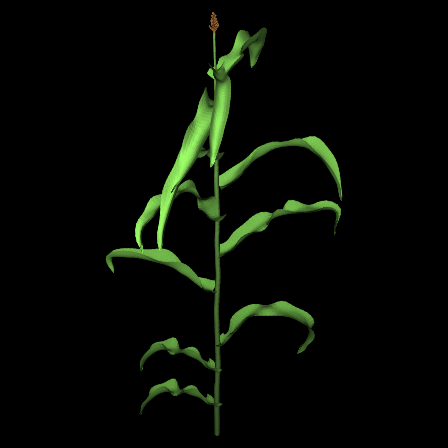
\includegraphics[width=0.2600in, height=0.2600in]{Figures/fig2/student_image.png}};
\node[anchor=south west, inner sep=0] at (4.1750,1.6200) {
\includegraphics[width=0.2600in, height=0.2600in]{Figures/fig2/student_hidden_0.png}};
\node[anchor=south west, inner sep=0] at (4.4750,1.6200) {
\includegraphics[width=0.2600in, height=0.2600in]{Figures/fig2/student_hidden_1.png}};
\node[anchor=south west, inner sep=0] at (4.7750,1.6200) {
\includegraphics[width=0.2600in, height=0.2600in]{Figures/fig2/student_hidden_2.png}};
\node[anchor=south west, inner sep=0] at (5.2650,1.6400) {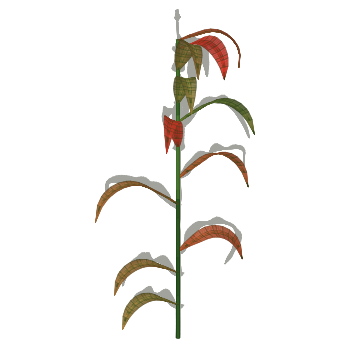
\includegraphics[width=0.5800in, height=0.5800in]{Figures/fig2/stage_2_before_recipe.png}};
\node[anchor=south west, inner sep=0] at (5.8850,1.6400) {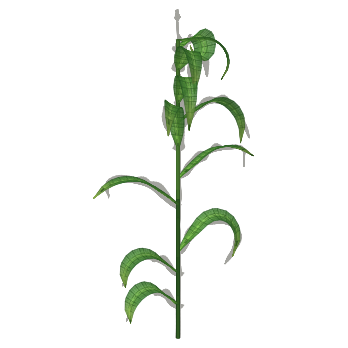
\includegraphics[width=0.5800in, height=0.5800in]{Figures/fig2/stage_2_after_recipe.png}};
\node[anchor=south west, inner sep=0] at (2.0350,0.4400) {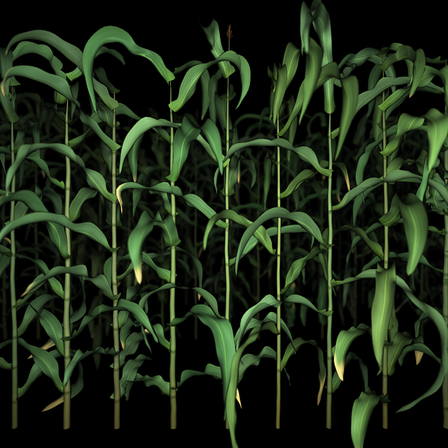
\includegraphics[width=0.4000in, height=0.4000in]{Figures/fig2/row_image.png}};
\node[anchor=south west, inner sep=0] at (2.4750,0.4400) {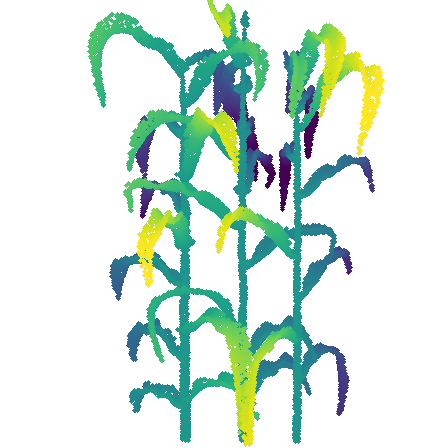
\includegraphics[width=0.4000in, height=0.4000in]{Figures/fig2/row_depth.png}};
\node[anchor=south west, inner sep=0] at (2.9150,0.4400) {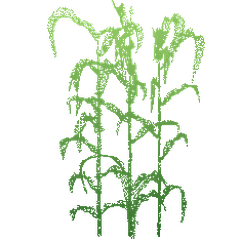
\includegraphics[width=0.4000in, height=0.4000in]{Figures/fig2/row_cloud.png}};
\node[anchor=south west, inner sep=0] at (4.2800,0.7250) {
\includegraphics[width=0.1700in, height=0.1700in]{Figures/fig2/fire_3.png}};
\node[anchor=south west, inner sep=0] at (5.2650,0.3800) {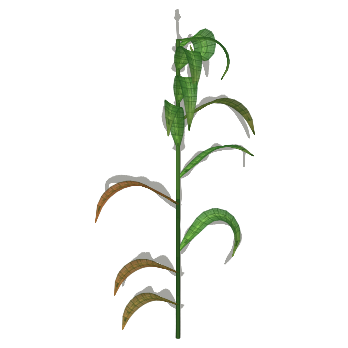
\includegraphics[width=0.5800in, height=0.5800in]{Figures/fig2/stage_3_before_recipe.png}};
\node[anchor=south west, inner sep=0] at (5.8850,0.3800) {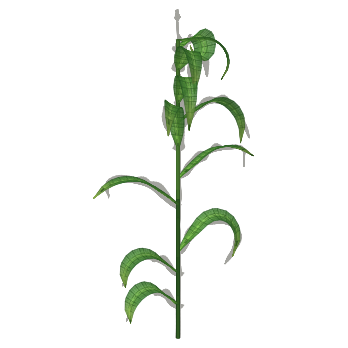
\includegraphics[width=0.5800in, height=0.5800in]{Figures/fig2/stage_3_after_recipe.png}};
\node[anchor=west, inner sep=0, outer sep=0, align=left, text=c1D221C, font={\fontsize{9.00}{11.25}\selectfont\sffamily\bfseries}] at (2.1450,4.2800) {Stage 1: Masked Pretraining};
\node[anchor=west, inner sep=0, outer sep=0, align=left, text=c1D221C, font={\fontsize{9.00}{11.25}\selectfont\sffamily\bfseries}] at (2.1450,2.5600) {Stage 2: Cross-Modal Distillation};
\node[anchor=west, inner sep=0, outer sep=0, align=left, text=c1D221C, font={\fontsize{9.00}{11.25}\selectfont\sffamily\bfseries}] at (2.1450,1.2400) {Stage 3: Row Fine-Tuning};
\draw[draw=cC0392B, line width=1.500pt, -{Triangle[length=5.00pt,width=4.60pt]}] (6.5000,3.4000) .. controls (6.7053,2.9333) and (6.7053,2.4667) .. (6.5000,2.0000);
\draw[draw=cC0392B, line width=1.500pt, -{Triangle[length=5.00pt,width=4.60pt]}] (6.5000,3.2000) .. controls (6.6863,2.3533) and (6.6863,1.5067) .. (6.5000,0.6600);
\node[anchor=center, inner sep=0, outer sep=0, align=center, text=cC0392B, font={\fontsize{9.00}{11.25}\selectfont\sffamily\bfseries}, rotate=90] at (6.8000,2.0000) {Warm Start};
\draw[draw=cC0392B, line width=0.800pt, rounded corners=0.0300in] (2.0350,3.4600) rectangle (2.4350,3.8600);
\draw[draw=cB8860B, line width=0.800pt, rounded corners=0.0300in] (2.4650,3.4600) rectangle (2.8650,3.8600);
\draw[draw=c2A9D8F, line width=0.800pt, rounded corners=0.0300in] (2.0350,3.0300) rectangle (2.4350,3.4300);
\draw[draw=c30638E, line width=0.800pt, rounded corners=0.0300in] (2.4650,3.0300) rectangle (2.8650,3.4300);
\draw[draw=cC0392B, line width=0.800pt, rounded corners=0.0300in] (3.0650,3.4600) rectangle (3.4650,3.8600);
\draw[draw=cB8860B, line width=0.800pt, rounded corners=0.0300in] (3.4950,3.4600) rectangle (3.8950,3.8600);
\draw[draw=c2A9D8F, line width=0.800pt, rounded corners=0.0300in] (3.0650,3.0300) rectangle (3.4650,3.4300);
\draw[draw=c30638E, line width=0.800pt, rounded corners=0.0300in] (3.4950,3.0300) rectangle (3.8950,3.4300);
\draw[draw=cC0392B, line width=0.800pt, rounded corners=0.0300in] (5.5750,3.4600) rectangle (5.9750,3.8600);
\draw[draw=cB8860B, line width=0.800pt, rounded corners=0.0300in] (6.0050,3.4600) rectangle (6.4050,3.8600);
\draw[draw=c2A9D8F, line width=0.800pt, rounded corners=0.0300in] (5.5750,3.0300) rectangle (5.9750,3.4300);
\draw[draw=c30638E, line width=0.800pt, rounded corners=0.0300in] (6.0050,3.0300) rectangle (6.4050,3.4300);
\node[anchor=south, inner sep=0, outer sep=0, align=center, text=c1D221C, font={\fontsize{9.00}{11.25}\selectfont\sffamily\bfseries}] at (2.4500,3.9600) {Input};
\node[anchor=south, inner sep=0, outer sep=0, align=center, text=c1D221C, font={\fontsize{9.00}{11.25}\selectfont\sffamily\bfseries}] at (3.4800,3.9600) {80 \% masked};
\node[anchor=south, inner sep=0, outer sep=0, align=center, text=c1D221C, font={\fontsize{9.00}{11.25}\selectfont\sffamily\bfseries}] at (5.9900,3.9600) {Output};
\draw[draw=c1D221C, line width=1.100pt, -{Triangle[length=4.20pt,width=4.00pt]}] (2.8950,3.4450) -- (3.0350,3.4450);
\draw[draw=c1D221C, line width=1.100pt, -{Triangle[length=4.20pt,width=4.00pt]}] (3.9250,3.4450) -- (4.1050,3.4450);
\node[anchor=center, inner sep=0, outer sep=0, align=center, text=c2B3A67, font={\fontsize{9.00}{11.25}\selectfont\sffamily\bfseries}] at (4.4443,3.4450) {Encoder};
\node[anchor=center, inner sep=0, outer sep=0, align=center, text=c2B3A67, font={\fontsize{9.00}{11.25}\selectfont\sffamily\bfseries}] at (5.1287,3.4450) {Decoder};
\draw[draw=c1D221C, line width=1.100pt, -{Triangle[length=4.20pt,width=4.00pt]}] (5.4450,3.4450) -- (5.5450,3.4450);
\draw[draw=cC0392B, line width=1.100pt, -{Triangle[length=4.20pt,width=4.00pt]}, dash pattern=on 2.70pt off 1.80pt] (5.9900,2.9500) -- (2.4500,2.9500);
\node[anchor=north, inner sep=0, outer sep=0, align=center, text=cC0392B, font={\fontsize{9.00}{11.25}\selectfont\sffamily}] at (4.2050,2.9000) {Loss on the masked tokens};
\node[anchor=west, inner sep=0, outer sep=0, align=left, text=c1D221C, font={\fontsize{9.00}{11.25}\selectfont\sffamily\bfseries}] at (2.3150,2.1100) {Teacher};
\draw[draw=cC0392B, line width=0.600pt, rounded corners=0.0300in] (2.0950,1.6200) rectangle (2.3550,1.8800);
\draw[draw=cB8860B, line width=0.600pt, rounded corners=0.0300in] (2.3950,1.6200) rectangle (2.6550,1.8800);
\draw[draw=c2A9D8F, line width=0.600pt, rounded corners=0.0300in] (2.6950,1.6200) rectangle (2.9550,1.8800);
\draw[draw=c30638E, line width=0.600pt, rounded corners=0.0300in] (2.9950,1.6200) rectangle (3.2550,1.8800);
\draw[draw=cC0392B, line width=1.100pt, -{Triangle[length=4.20pt,width=4.00pt]}, dash pattern=on 2.70pt off 1.80pt] (3.3150,1.8800) -- (3.7850,1.8800);
\node[anchor=south, inner sep=0, outer sep=0, align=center, text=cC0392B, font={\fontsize{9.00}{11.25}\selectfont\sffamily}] at (3.5500,1.9300) {Features};
\node[anchor=west, inner sep=0, outer sep=0, align=left, text=c2B3A67, font={\fontsize{9.00}{11.25}\selectfont\sffamily\bfseries}] at (4.0950,2.1100) {Student};
\draw[draw=cC0392B, line width=0.900pt, rounded corners=0.0300in] (3.8750,1.6200) rectangle (4.1350,1.8800);
\draw[draw=cB8860B, line width=0.600pt, dash pattern=on 1.80pt off 1.20pt, rounded corners=0.0300in] (4.1750,1.6200) rectangle (4.4350,1.8800);
\draw[draw=c2A9D8F, line width=0.600pt, dash pattern=on 1.80pt off 1.20pt, rounded corners=0.0300in] (4.4750,1.6200) rectangle (4.7350,1.8800);
\draw[draw=c30638E, line width=0.600pt, dash pattern=on 1.80pt off 1.20pt, rounded corners=0.0300in] (4.7750,1.6200) rectangle (5.0350,1.8800);
\draw[draw=c1D221C, line width=1.100pt, -{Triangle[length=4.20pt,width=4.00pt]}] (5.0950,1.9100) -- (5.2350,1.9100);
\draw[draw=c5F685C, line width=0.800pt, dash pattern=on 2.40pt off 1.60pt, rounded corners=0.0300in] (5.2650,1.6400) rectangle (5.8450,2.2200);
\node[anchor=south, inner sep=0, outer sep=0, align=center, text=c5F685C, font={\fontsize{9.00}{11.25}\selectfont\sffamily}] at (5.5550,2.2700) {Before};
\draw[draw=c30638E, line width=0.800pt, rounded corners=0.0300in] (5.8850,1.6400) rectangle (6.4650,2.2200);
\node[anchor=south, inner sep=0, outer sep=0, align=center, text=c2B3A67, font={\fontsize{9.00}{11.25}\selectfont\sffamily\bfseries}] at (6.1750,2.2700) {After};
\node[anchor=north, inner sep=0, outer sep=0, align=center, text=c1D221C, font={\fontsize{9.00}{11.25}\selectfont\sffamily}] at (5.8250,1.5800) {$\theta$ MAE 0.058 $\rightarrow$ 0.014};
\draw[draw=cC0392B, line width=0.800pt, rounded corners=0.0300in] (2.0350,0.4400) rectangle (2.4350,0.8400);
\draw[draw=cB8860B, line width=0.800pt, rounded corners=0.0300in] (2.4750,0.4400) rectangle (2.8750,0.8400);
\draw[draw=c2A9D8F, line width=0.800pt, rounded corners=0.0300in] (2.9150,0.4400) rectangle (3.3150,0.8400);
\node[anchor=south, inner sep=0, outer sep=0, align=center, text=c1D221C, font={\fontsize{9.00}{11.25}\selectfont\sffamily\bfseries}] at (2.6750,0.9200) {Crop Row};
\draw[draw=c1D221C, line width=1.100pt, -{Triangle[length=4.20pt,width=4.00pt]}] (3.3650,0.6400) -- (3.7150,0.6400);
\node[anchor=center, inner sep=0, outer sep=0, align=center, text=c2B3A67, font={\fontsize{9.00}{11.25}\selectfont\sffamily\bfseries}] at (4.0344,0.6400) {Enc};
\node[anchor=center, inner sep=0, outer sep=0, align=center, text=c2B3A67, font={\fontsize{9.00}{11.25}\selectfont\sffamily\bfseries}] at (4.6771,0.6400) {Dec};
\node[anchor=north, inner sep=0, outer sep=0, align=center, text=cC0392B, font={\fontsize{9.00}{11.25}\selectfont\sffamily}] at (4.3450,0.3500) {Loss: Target Plant Only};
\draw[draw=c1D221C, line width=1.100pt, -{Triangle[length=4.20pt,width=4.00pt]}] (4.9750,0.6400) -- (5.2350,0.6400);
\draw[draw=c5F685C, line width=0.800pt, dash pattern=on 2.40pt off 1.60pt, rounded corners=0.0300in] (5.2650,0.3800) rectangle (5.8450,0.9600);
\node[anchor=south, inner sep=0, outer sep=0, align=center, text=c5F685C, font={\fontsize{9.00}{11.25}\selectfont\sffamily}] at (5.5550,1.0100) {Before};
\draw[draw=c30638E, line width=0.800pt, rounded corners=0.0300in] (5.8850,0.3800) rectangle (6.4650,0.9600);
\node[anchor=south, inner sep=0, outer sep=0, align=center, text=c2B3A67, font={\fontsize{9.00}{11.25}\selectfont\sffamily\bfseries}] at (6.1750,1.0100) {After};
\node[anchor=north, inner sep=0, outer sep=0, align=center, text=c1D221C, font={\fontsize{9.00}{11.25}\selectfont\sffamily}] at (5.8250,0.3200) {$\theta$ MAE 0.114 $\rightarrow$ 0.061};
\node[anchor=center, inner sep=0, outer sep=0, align=center, text=c1D221C, font={\fontsize{11.00}{11.25}\selectfont\sffamily\bfseries}] at (0.8975,4.0600) {CropCode};
\node[anchor=west, inner sep=0, outer sep=0, align=left, text=cC0392B, font={\fontsize{9.00}{11.25}\selectfont\sffamily\bfseries}] at (0.8450,3.7100) {Image  196 \\ tokens};
\node[anchor=west, inner sep=0, outer sep=0, align=left, text=cB8860B, font={\fontsize{9.00}{11.25}\selectfont\sffamily\bfseries}] at (0.8450,3.4100) {Depth  196\\ tokens };
\node[anchor=west, inner sep=0, outer sep=0, align=left, text=c2A9D8F, font={\fontsize{9.00}{11.25}\selectfont\sffamily\bfseries}] at (0.8450,3.1100) {Point Cloud \\ 196 tokens};
\node[anchor=west, inner sep=0, outer sep=0, align=left, text=c30638E, font={\fontsize{9.00}{11.25}\selectfont\sffamily\bfseries}] at (0.8450,2.8100) {Params  1+K \\ tokens};
\node[anchor=center, inner sep=0, outer sep=0, align=center,
text=c5F685C, font={\fontsize{9.00}{11.25}\selectfont\sffamily}]
at (0.8975,2.5200) {Missing Tokens = Masked};
\node[anchor=center, inner sep=0, outer sep=0,
align=center, text=c1D221C,
font={\fontsize{8.00}{11.25}\selectfont\sffamily\bfseries}]
at (0.8975,2.2000) {Dirichlet Split};
\node[anchor=center, inner sep=0, outer sep=0,
align=center, text=c5F685C,
font={\fontsize{9.00}{11.25}\selectfont\sffamily}]
at (0.8975,1.7600) {Visible Tokens};
\node[anchor=center, inner sep=0, outer sep=0, align=center, text=c2B3A67, font={\fontsize{9.00}{11.25}\selectfont\sffamily\bfseries}] at (0.8975,1.2700) {Encoder, 12 Blocks};
\node[anchor=center, inner sep=0, outer sep=0, align=center, text=c2B3A67, font={\fontsize{9.00}{11.25}\selectfont\sffamily\bfseries}] at (0.8975,0.7100) {Decoder, 8 Blocks};
\draw[draw=c2B3A67, line width=1.000pt, -{Triangle[length=4.00pt,width=3.80pt]}] (0.8975,1.6200) -- (0.8975,1.4900);
\draw[draw=c2B3A67, line width=1.000pt, -{Triangle[length=4.00pt,width=3.80pt]}] (0.8975,1.0500) -- (0.8975,0.9300);
\draw[draw=c2B3A67, line width=1.000pt, -{Triangle[length=4.00pt,width=3.80pt]}] (0.8975,0.4900) -- (0.8975,0.4200);
\node[anchor=center, inner sep=0, outer sep=0, align=center, text=c2B3A67, font={\fontsize{9.00}{11.25}\selectfont\sffamily}] at (0.8975,0.3200) {One Head Per Stream};
\end{tikzpicture}%
}%
}
      \vspace{-15pt}

    \caption{\textbf{Training of \method{}: Pretraining and two parallel specializations.}
    \textbf{Stage~1:} Four streams (RGB, depth, point cloud, procedural parameters) undergo 80\% Dirichlet-allocated masking and shared encoder-decoder reconstruction.
    \textbf{Stage~2:} A frozen four-stream teacher transfers its latent representation and decoder features to single-modality students.
    \textbf{Stage~3:} The Stage~1 model is fine-tuned on simulated rows with supervision on the occluded target plant only.
    Reported values compare sorghum parameter MAE from RGB before and after distillation (Stage~2) and leaf-parameter MAE on rows using all streams before and after fine-tuning (Stage~3, \tabref{tab:rows-main}).}
  \label{fig:arch}
\end{figure*}


%%%%%%%%%%%%%%%%%%%%%%%%%%%%%%%%%%%%%%%%%%%%%%%%%%%%%%%%%%%%%%%%%%%%%%%%%%%
% 3. METHOD
%%%%%%%%%%%%%%%%%%%%%%%%%%%%%%%%%%%%%%%%%%%%%%%%%%%%%%%%%%%%%%%%%%%%%%%%%%%
\section{Method}
\label{sec:method}

\subsection{Problem Formulation}
\label{sec:method-form}

Let $G$ denote a species-specific procedural plant generator that maps a compact parameter vector $\theta \in \R^{d_\theta}$ to an editable 3D mesh $G(\theta)$. The vector $\theta$ (also called the plant's recipe) specifies global traits such as stem height and internode spacing, and per-leaf attributes including insertion height, blade length and width, and insertion, roll, and azimuth angles. A rover-mounted sensor provides a partial, noisy, and occluded observation from a subset of modalities $S \subseteq \mathcal{M} = \{\mathrm{rgb}, \mathrm{d}, \mathrm{pc}\}$, where $\mathrm{rgb}$ denotes a color image, $\mathrm{d}$ a metric depth map, and $\mathrm{pc}$ a 3D point cloud. Our goal is to learn an amortized feed-forward inverse mapping,
\begin{equation}
  f_\phi\!\left(\{x^m : m \in S\}\right)
  = \left(\hat\theta, \{\hat x^m : m \in \mathcal{M}\}\right)
  \label{eq:procedural-inverse}
\end{equation}
that predicts both the complete procedural parameter vector $\hat\theta$ and the completed sensor streams $\{\hat x^m\}$ in a single forward pass. The parameter vector, $\hat\theta$, is the output of interest. Predicting $\hat\theta$ uses $G$ as an explicit biological prior, and re-rendering $G(\hat\theta)$ produces watertight, structurally valid, and editable 3D geometry in milliseconds.

\subsection{A Procedural Field-Data Engine: \dataset{}}
\label{sec:method-data}

To train and benchmark \method{} under controlled yet realistic conditions, we build \dataset{}, a dataset that pairs exact procedural ground truth with multimodal captures of isolated plants and densely planted crop rows (\figref{fig:dataset}, \tabref{tab:datacompare}, and additional tables in the Appendix).
% APPENDIX REF (removed for submission, restore later): \tabref{tab:fieldproc} in \appendixref{app:data} (for: additional tables in Appendix)

\begin{figure*}[t]
  \centering
  \resizebox{\linewidth}{!}{% Fig. 3 (the dataset) as native TikZ, written by figures/make_dataset_fig_v2.py (do not edit by hand: re-run it).
% Tiles in Figures/fig3/; boxes, leader lines and text are TikZ, text in \sffamily (Helvetica under cvpr/times).
% Natural size 6.875 x 3.86 in; include with \resizebox{\textwidth}{!}{% Fig. 3 (the dataset) as native TikZ, written by figures/make_dataset_fig_v2.py (do not edit by hand: re-run it).
% Tiles in Figures/fig3/; boxes, leader lines and text are TikZ, text in \sffamily (Helvetica under cvpr/times).
% Natural size 6.875 x 3.86 in; include with \resizebox{\textwidth}{!}{% Fig. 3 (the dataset) as native TikZ, written by figures/make_dataset_fig_v2.py (do not edit by hand: re-run it).
% Tiles in Figures/fig3/; boxes, leader lines and text are TikZ, text in \sffamily (Helvetica under cvpr/times).
% Natural size 6.875 x 3.86 in; include with \resizebox{\textwidth}{!}{\input{Figures/fig_dataset_tikz}}.
\definecolor{c111111}{HTML}{111111}%
\definecolor{c333333}{HTML}{333333}%
\definecolor{c3F5F8F}{HTML}{3F5F8F}%
\definecolor{c444444}{HTML}{444444}%
\definecolor{c555555}{HTML}{555555}%
\definecolor{c5E4A96}{HTML}{5E4A96}%
\definecolor{c809EC2}{HTML}{809EC2}%
\definecolor{c9A9A9A}{HTML}{9A9A9A}%
\definecolor{c9D8CC4}{HTML}{9D8CC4}%
\definecolor{cA07800}{HTML}{A07800}%
\definecolor{cA8456E}{HTML}{A8456E}%
\definecolor{cD091A7}{HTML}{D091A7}%
\definecolor{cE0B020}{HTML}{E0B020}%
\definecolor{cE6ECF3}{HTML}{E6ECF3}%
\definecolor{cEAE7F2}{HTML}{EAE7F2}%
\definecolor{cF4F4F5}{HTML}{F4F4F5}%
\definecolor{cF6E9ED}{HTML}{F6E9ED}%
\definecolor{cFAF2D4}{HTML}{FAF2D4}%
\begin{tikzpicture}[x=1in, y=1in]
\useasboundingbox (0,0) rectangle (6.875,3.86);
\node[anchor=base west, inner sep=0, text=c111111, rotate=0, font={\fontsize{9.0}{10.8}\selectfont\sffamily\bfseries}] at (0.0200,3.7200) {a};
\node[anchor=base west, inner sep=0, text=c111111, rotate=0, font={\fontsize{6.2}{7.4}\selectfont\sffamily}] at (0.1800,3.7200) {The plants: \textbf{15,000} per species.};
\node[anchor=base west, inner sep=0, text=c111111, rotate=0, font={\fontsize{9.0}{10.8}\selectfont\sffamily\bfseries}] at (2.3800,3.7200) {b};
\node[anchor=base west, inner sep=0, text=c111111, rotate=0, font={\fontsize{6.2}{7.4}\selectfont\sffamily}] at (2.5400,3.7200) {One view of the boxed plant as its four streams};
\draw[draw=c809EC2, line width=1.00pt, rounded corners=4.32pt, fill=cE6ECF3] (0.2400,2.4100) rectangle (1.7500,3.4450);
\node[anchor=center, inner sep=0, text=c111111, rotate=90, font={\fontsize{7.0}{8.4}\selectfont\sffamily\bfseries}] at (0.1500,2.9275) {Sorghum};
\node[anchor=south west, inner sep=0] at (0.3000,2.9450) {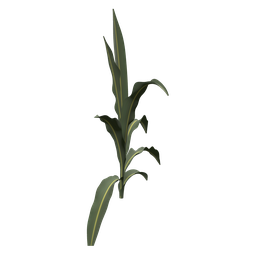
\includegraphics[width=0.4400in, height=0.4400in]{Figures/fig3/sorghum_gallery_0.png}};
\node[anchor=south west, inner sep=0] at (0.7750,2.9450) {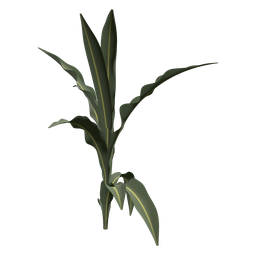
\includegraphics[width=0.4400in, height=0.4400in]{Figures/fig3/sorghum_gallery_1.png}};
\node[anchor=south west, inner sep=0] at (1.2500,2.9450) {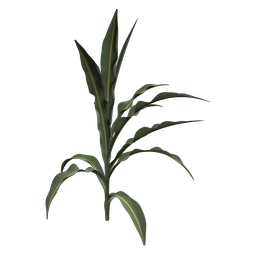
\includegraphics[width=0.4400in, height=0.4400in]{Figures/fig3/sorghum_gallery_2.png}};
\node[anchor=south west, inner sep=0] at (0.3000,2.4700) {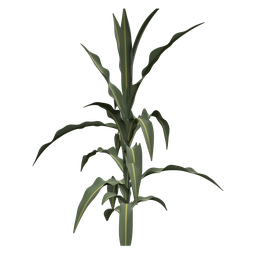
\includegraphics[width=0.4400in, height=0.4400in]{Figures/fig3/sorghum_gallery_3.png}};
\node[anchor=south west, inner sep=0] at (0.7750,2.4700) {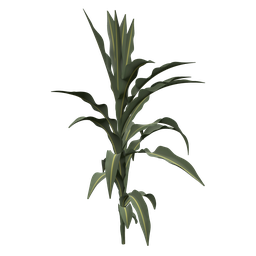
\includegraphics[width=0.4400in, height=0.4400in]{Figures/fig3/sorghum_gallery_4.png}};
\node[anchor=south west, inner sep=0] at (1.2500,2.4700) {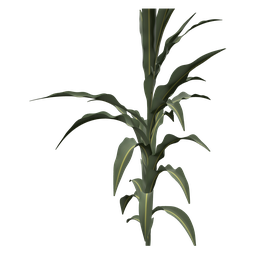
\includegraphics[width=0.4400in, height=0.4400in]{Figures/fig3/sorghum_gallery_5.png}};
\draw[draw=c333333, line width=1.00pt, rounded corners=2.16pt] (1.2350,2.4550) rectangle (1.7050,2.9250);
\draw[draw=c9A9A9A, line width=0.60pt] (1.7050,2.9250) -- (2.3700,3.4175);
\draw[draw=c9A9A9A, line width=0.60pt] (1.7050,2.4550) -- (2.3700,2.4375);
\draw[draw=c9A9A9A, line width=1.00pt, rounded corners=4.32pt, fill=cF4F4F5] (2.3700,2.4375) rectangle (6.8050,3.4175);
\draw[draw=c809EC2, line width=1.00pt, rounded corners=3.60pt, fill=cE6ECF3] (2.4100,2.4775) rectangle (3.3100,3.3775);
\node[anchor=south west, inner sep=0] at (2.4400,2.5075) {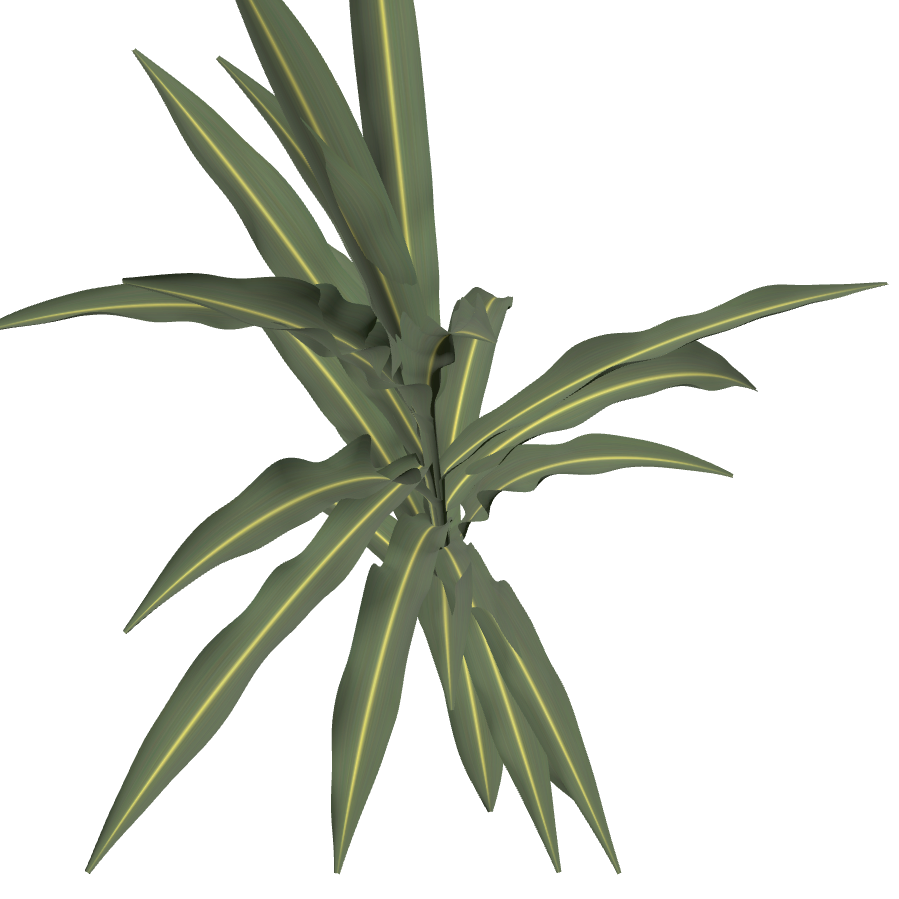
\includegraphics[width=0.8400in, height=0.8400in]{Figures/fig3/sorghum_rgb.png}};
\node[anchor=base, inner sep=0, text=c3F5F8F, rotate=0, font={\fontsize{6.2}{7.4}\selectfont\sffamily\bfseries}] at (2.8600,3.4925) {Image};
\draw[draw=cE0B020, line width=1.00pt, rounded corners=3.60pt, fill=cFAF2D4] (3.5617,2.4775) rectangle (4.4617,3.3775);
\node[anchor=south west, inner sep=0] at (3.5917,2.5075) {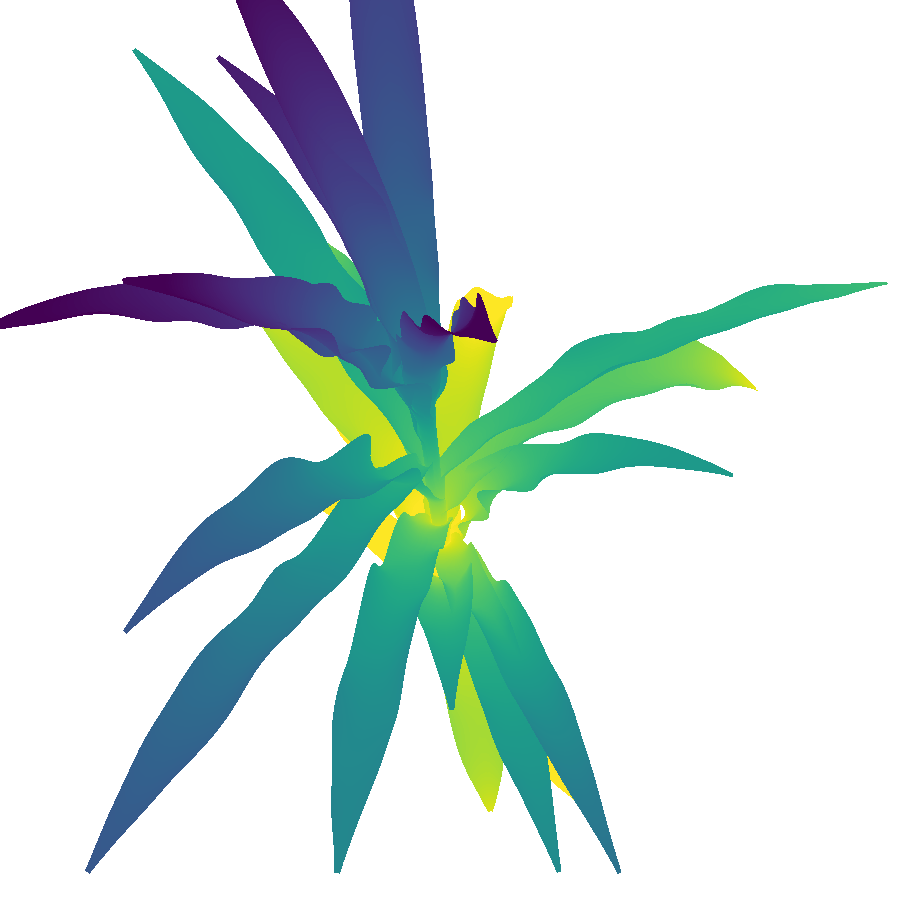
\includegraphics[width=0.8400in, height=0.8400in]{Figures/fig3/sorghum_depth.png}};
\node[anchor=base, inner sep=0, text=cA07800, rotate=0, font={\fontsize{6.2}{7.4}\selectfont\sffamily\bfseries}] at (4.0117,3.4925) {Depth image};
\draw[draw=cD091A7, line width=1.00pt, rounded corners=3.60pt, fill=cF6E9ED] (4.7133,2.4775) rectangle (5.6133,3.3775);
\node[anchor=south west, inner sep=0] at (4.7433,2.5075) {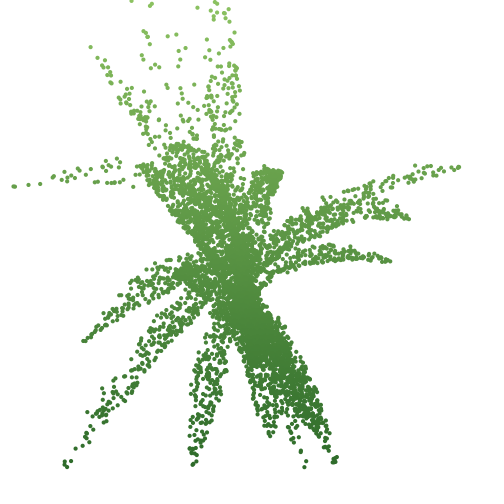
\includegraphics[width=0.8400in, height=0.8400in]{Figures/fig3/sorghum_pc.png}};
\node[anchor=base, inner sep=0, text=cA8456E, rotate=0, font={\fontsize{6.2}{7.4}\selectfont\sffamily\bfseries}] at (5.1633,3.4925) {Point Cloud};
\draw[draw=c9D8CC4, line width=1.00pt, rounded corners=3.60pt, fill=cEAE7F2] (5.8650,2.4775) rectangle (6.7650,3.3775);
\node[anchor=south west, inner sep=0] at (5.8950,2.5075) {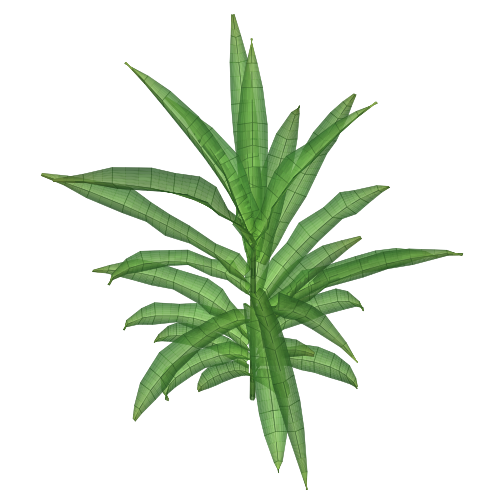
\includegraphics[width=0.8400in, height=0.8400in]{Figures/fig3/sorghum_text.png}};
\node[anchor=base, inner sep=0, text=c5E4A96, rotate=0, font={\fontsize{6.2}{7.4}\selectfont\sffamily\bfseries}] at (6.3150,3.4925) {Procedural Model};
\draw[draw=c809EC2, line width=1.00pt, rounded corners=4.32pt, fill=cE6ECF3] (0.2400,1.3100) rectangle (1.7500,2.3450);
\node[anchor=center, inner sep=0, text=c111111, rotate=90, font={\fontsize{7.0}{8.4}\selectfont\sffamily\bfseries}] at (0.1500,1.8275) {Maize};
\node[anchor=south west, inner sep=0] at (0.3000,1.8450) {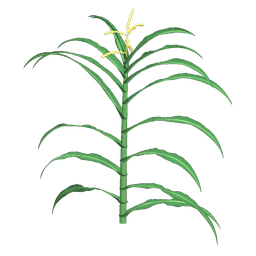
\includegraphics[width=0.4400in, height=0.4400in]{Figures/fig3/maize_gallery_0.png}};
\node[anchor=south west, inner sep=0] at (0.7750,1.8450) {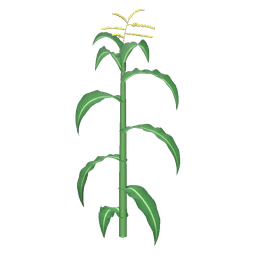
\includegraphics[width=0.4400in, height=0.4400in]{Figures/fig3/maize_gallery_1.png}};
\node[anchor=south west, inner sep=0] at (1.2500,1.8450) {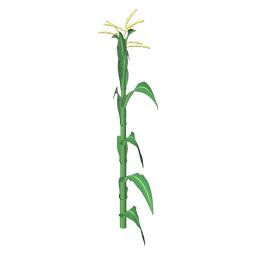
\includegraphics[width=0.4400in, height=0.4400in]{Figures/fig3/maize_gallery_2.png}};
\node[anchor=south west, inner sep=0] at (0.3000,1.3700) {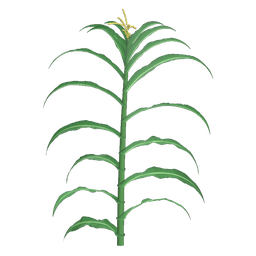
\includegraphics[width=0.4400in, height=0.4400in]{Figures/fig3/maize_gallery_3.png}};
\node[anchor=south west, inner sep=0] at (0.7750,1.3700) {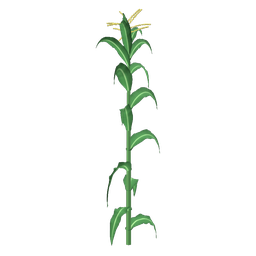
\includegraphics[width=0.4400in, height=0.4400in]{Figures/fig3/maize_gallery_4.png}};
\node[anchor=south west, inner sep=0] at (1.2500,1.3700) {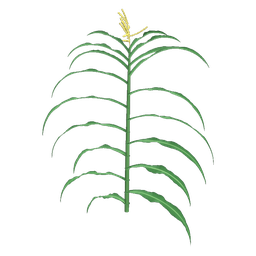
\includegraphics[width=0.4400in, height=0.4400in]{Figures/fig3/maize_gallery_5.png}};
\draw[draw=c333333, line width=1.00pt, rounded corners=2.16pt] (1.2350,1.3550) rectangle (1.7050,1.8250);
\draw[draw=c9A9A9A, line width=0.60pt] (1.7050,1.8250) -- (2.3700,2.3175);
\draw[draw=c9A9A9A, line width=0.60pt] (1.7050,1.3550) -- (2.3700,1.3375);
\draw[draw=c9A9A9A, line width=1.00pt, rounded corners=4.32pt, fill=cF4F4F5] (2.3700,1.3375) rectangle (6.8050,2.3175);
\draw[draw=c809EC2, line width=1.00pt, rounded corners=3.60pt, fill=cE6ECF3] (2.4100,1.3775) rectangle (3.3100,2.2775);
\node[anchor=south west, inner sep=0] at (2.4400,1.4075) {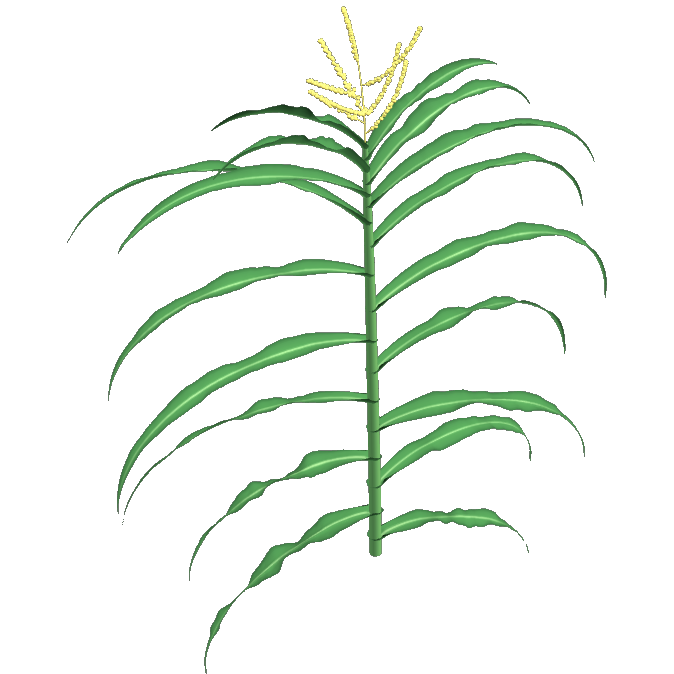
\includegraphics[width=0.8400in, height=0.8400in]{Figures/fig3/maize_rgb.png}};
\draw[draw=cE0B020, line width=1.00pt, rounded corners=3.60pt, fill=cFAF2D4] (3.5617,1.3775) rectangle (4.4617,2.2775);
\node[anchor=south west, inner sep=0] at (3.5917,1.4075) {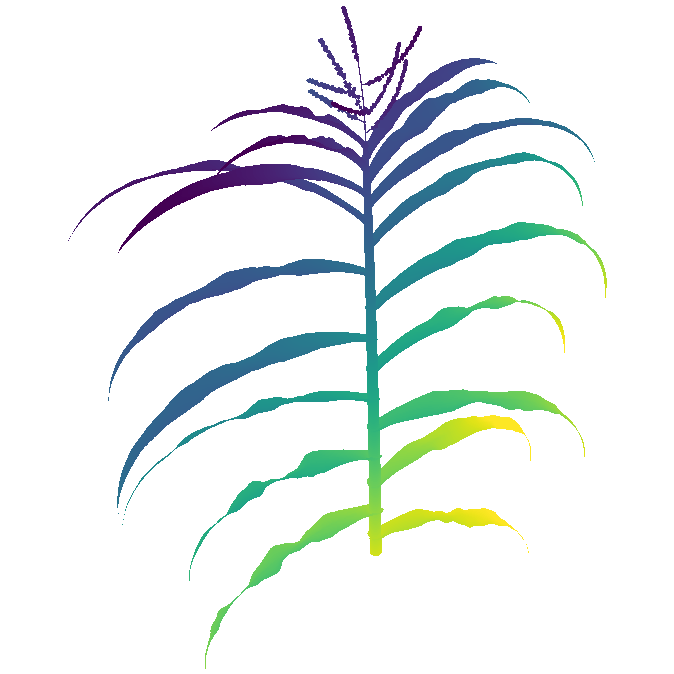
\includegraphics[width=0.8400in, height=0.8400in]{Figures/fig3/maize_depth.png}};
\draw[draw=cD091A7, line width=1.00pt, rounded corners=3.60pt, fill=cF6E9ED] (4.7133,1.3775) rectangle (5.6133,2.2775);
\node[anchor=south west, inner sep=0] at (4.7433,1.4075) {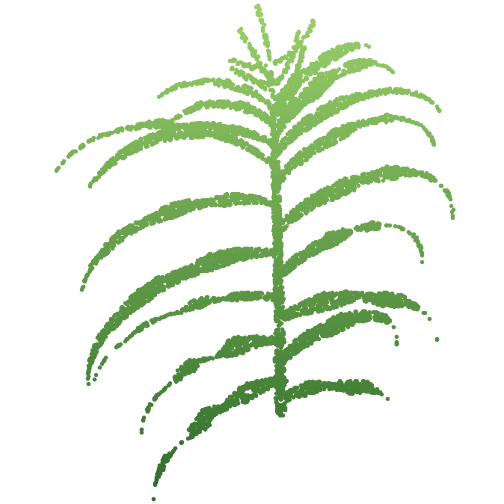
\includegraphics[width=0.8400in, height=0.8400in]{Figures/fig3/maize_pc.png}};
\draw[draw=c9D8CC4, line width=1.00pt, rounded corners=3.60pt, fill=cEAE7F2] (5.8650,1.3775) rectangle (6.7650,2.2775);
\node[anchor=south west, inner sep=0] at (5.8950,1.4075) {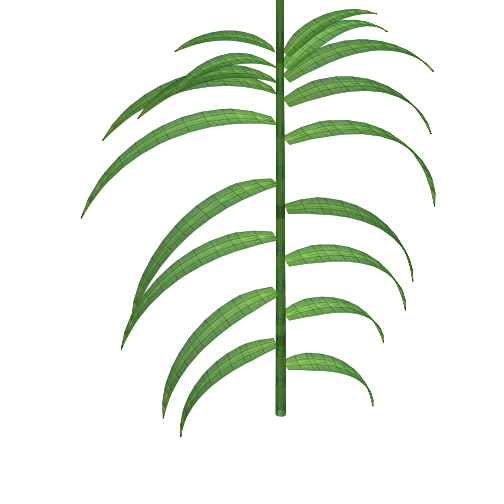
\includegraphics[width=0.8400in, height=0.8400in]{Figures/fig3/maize_text.png}};
\node[anchor=base west, inner sep=0, text=c111111, rotate=0, font={\fontsize{9.0}{10.8}\selectfont\sffamily\bfseries}] at (0.0200,1.1300) {c};
\node[anchor=base west, inner sep=0, text=c111111, rotate=0, font={\fontsize{6.2}{7.4}\selectfont\sffamily}] at (0.1800,1.1300) {Ten cameras per plant (five shown), by elevation};
\draw[draw=c809EC2, line width=1.00pt, rounded corners=2.88pt, fill=cE6ECF3] (0.2600,0.5600) rectangle (2.1800,0.9800);
\node[anchor=center, inner sep=0, text=c111111, rotate=90, font={\fontsize{5.8}{7.0}\selectfont\sffamily\bfseries}] at (0.1500,0.7700) {Sorghum};
\node[anchor=south west, inner sep=0] at (0.3000,0.6000) {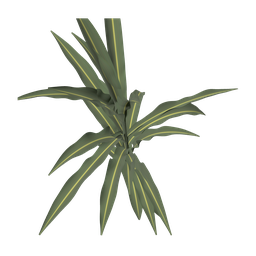
\includegraphics[width=0.3400in, height=0.3400in]{Figures/fig3/sorghum_camera_0.png}};
\node[anchor=south, inner sep=0, text=c444444, rotate=0, font={\fontsize{5.4}{6.5}\selectfont\sffamily}] at (0.4700,0.9900) {+64$^{\circ}$};
\node[anchor=south west, inner sep=0] at (0.6750,0.6000) {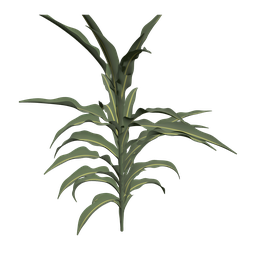
\includegraphics[width=0.3400in, height=0.3400in]{Figures/fig3/sorghum_camera_1.png}};
\node[anchor=south, inner sep=0, text=c444444, rotate=0, font={\fontsize{5.4}{6.5}\selectfont\sffamily}] at (0.8450,0.9900) {+30$^{\circ}$};
\node[anchor=south west, inner sep=0] at (1.0500,0.6000) {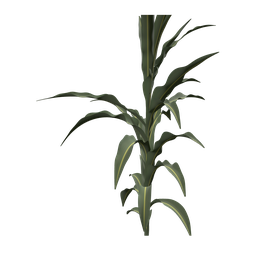
\includegraphics[width=0.3400in, height=0.3400in]{Figures/fig3/sorghum_camera_2.png}};
\node[anchor=south, inner sep=0, text=c444444, rotate=0, font={\fontsize{5.4}{6.5}\selectfont\sffamily}] at (1.2200,0.9900) {+6$^{\circ}$};
\node[anchor=south west, inner sep=0] at (1.4250,0.6000) {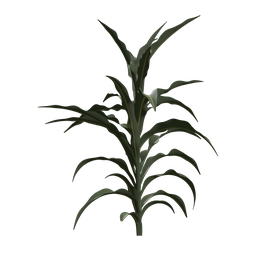
\includegraphics[width=0.3400in, height=0.3400in]{Figures/fig3/sorghum_camera_3.png}};
\node[anchor=south, inner sep=0, text=c444444, rotate=0, font={\fontsize{5.4}{6.5}\selectfont\sffamily}] at (1.5950,0.9900) {$-$17$^{\circ}$};
\node[anchor=south west, inner sep=0] at (1.8000,0.6000) {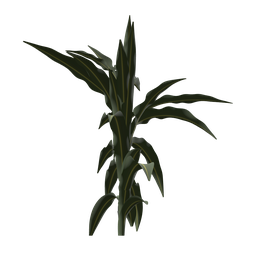
\includegraphics[width=0.3400in, height=0.3400in]{Figures/fig3/sorghum_camera_4.png}};
\node[anchor=south, inner sep=0, text=c444444, rotate=0, font={\fontsize{5.4}{6.5}\selectfont\sffamily}] at (1.9700,0.9900) {$-$44$^{\circ}$};
\draw[draw=c809EC2, line width=1.00pt, rounded corners=2.88pt, fill=cE6ECF3] (0.2600,0.0300) rectangle (2.1800,0.4500);
\node[anchor=center, inner sep=0, text=c111111, rotate=90, font={\fontsize{5.8}{7.0}\selectfont\sffamily\bfseries}] at (0.1500,0.2400) {Maize};
\node[anchor=south west, inner sep=0] at (0.3000,0.0700) {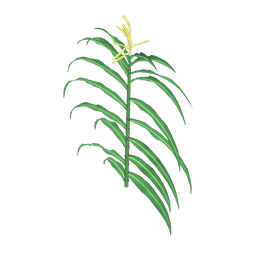
\includegraphics[width=0.3400in, height=0.3400in]{Figures/fig3/maize_camera_0.png}};
\node[anchor=south, inner sep=0, text=c444444, rotate=0, font={\fontsize{5.4}{6.5}\selectfont\sffamily}] at (0.4700,0.4600) {+39$^{\circ}$};
\node[anchor=south west, inner sep=0] at (0.6750,0.0700) {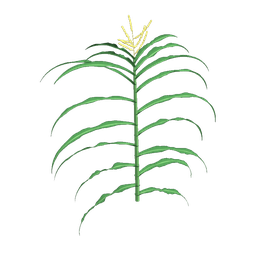
\includegraphics[width=0.3400in, height=0.3400in]{Figures/fig3/maize_camera_1.png}};
\node[anchor=south, inner sep=0, text=c444444, rotate=0, font={\fontsize{5.4}{6.5}\selectfont\sffamily}] at (0.8450,0.4600) {+30$^{\circ}$};
\node[anchor=south west, inner sep=0] at (1.0500,0.0700) {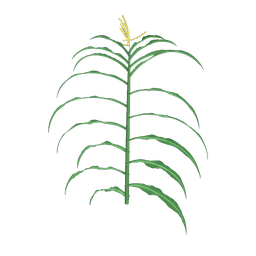
\includegraphics[width=0.3400in, height=0.3400in]{Figures/fig3/maize_camera_2.png}};
\node[anchor=south, inner sep=0, text=c444444, rotate=0, font={\fontsize{5.4}{6.5}\selectfont\sffamily}] at (1.2200,0.4600) {+10$^{\circ}$};
\node[anchor=south west, inner sep=0] at (1.4250,0.0700) {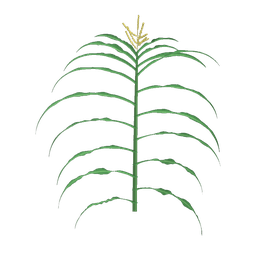
\includegraphics[width=0.3400in, height=0.3400in]{Figures/fig3/maize_camera_3.png}};
\node[anchor=south, inner sep=0, text=c444444, rotate=0, font={\fontsize{5.4}{6.5}\selectfont\sffamily}] at (1.5950,0.4600) {$-$13$^{\circ}$};
\node[anchor=south west, inner sep=0] at (1.8000,0.0700) {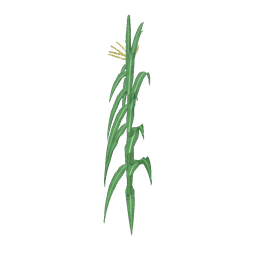
\includegraphics[width=0.3400in, height=0.3400in]{Figures/fig3/maize_camera_4.png}};
\node[anchor=south, inner sep=0, text=c444444, rotate=0, font={\fontsize{5.4}{6.5}\selectfont\sffamily}] at (1.9700,0.4600) {$-$36$^{\circ}$};
\node[anchor=base west, inner sep=0, text=c111111, rotate=0, font={\fontsize{9.0}{10.8}\selectfont\sffamily\bfseries}] at (2.8400,1.1300) {d};
\node[anchor=base west, inner sep=0, text=c111111, rotate=0, font={\fontsize{6.2}{7.4}\selectfont\sffamily}] at (3.0000,1.1300) {Crop rows: the target plant between neighbors};
\node[anchor=base west, inner sep=0, text=c555555, rotate=0, font={\fontsize{5.4}{6.5}\selectfont\sffamily}] at (3.0000,1.0250) {\textcolor{cLegRed}{\textbf{Red}}: Neighbor pixels  \textcolor{cLegOrange}{\textbf{Orange}}: Target pixels occluded by neighbors (\% hidden)  \textcolor{cLegGreen}{\textbf{Green}}: Target points};
\node[anchor=base, inner sep=0, text=c111111, rotate=0, font={\fontsize{6.2}{7.4}\selectfont\sffamily\bfseries}] at (3.7600,0.9350) {Sorghum};
\draw[draw=c809EC2, line width=1.00pt, rounded corners=3.60pt, fill=cE6ECF3] (2.9900,0.1300) rectangle (3.7500,0.8900);
\node[anchor=south west, inner sep=0] at (3.0200,0.1600) {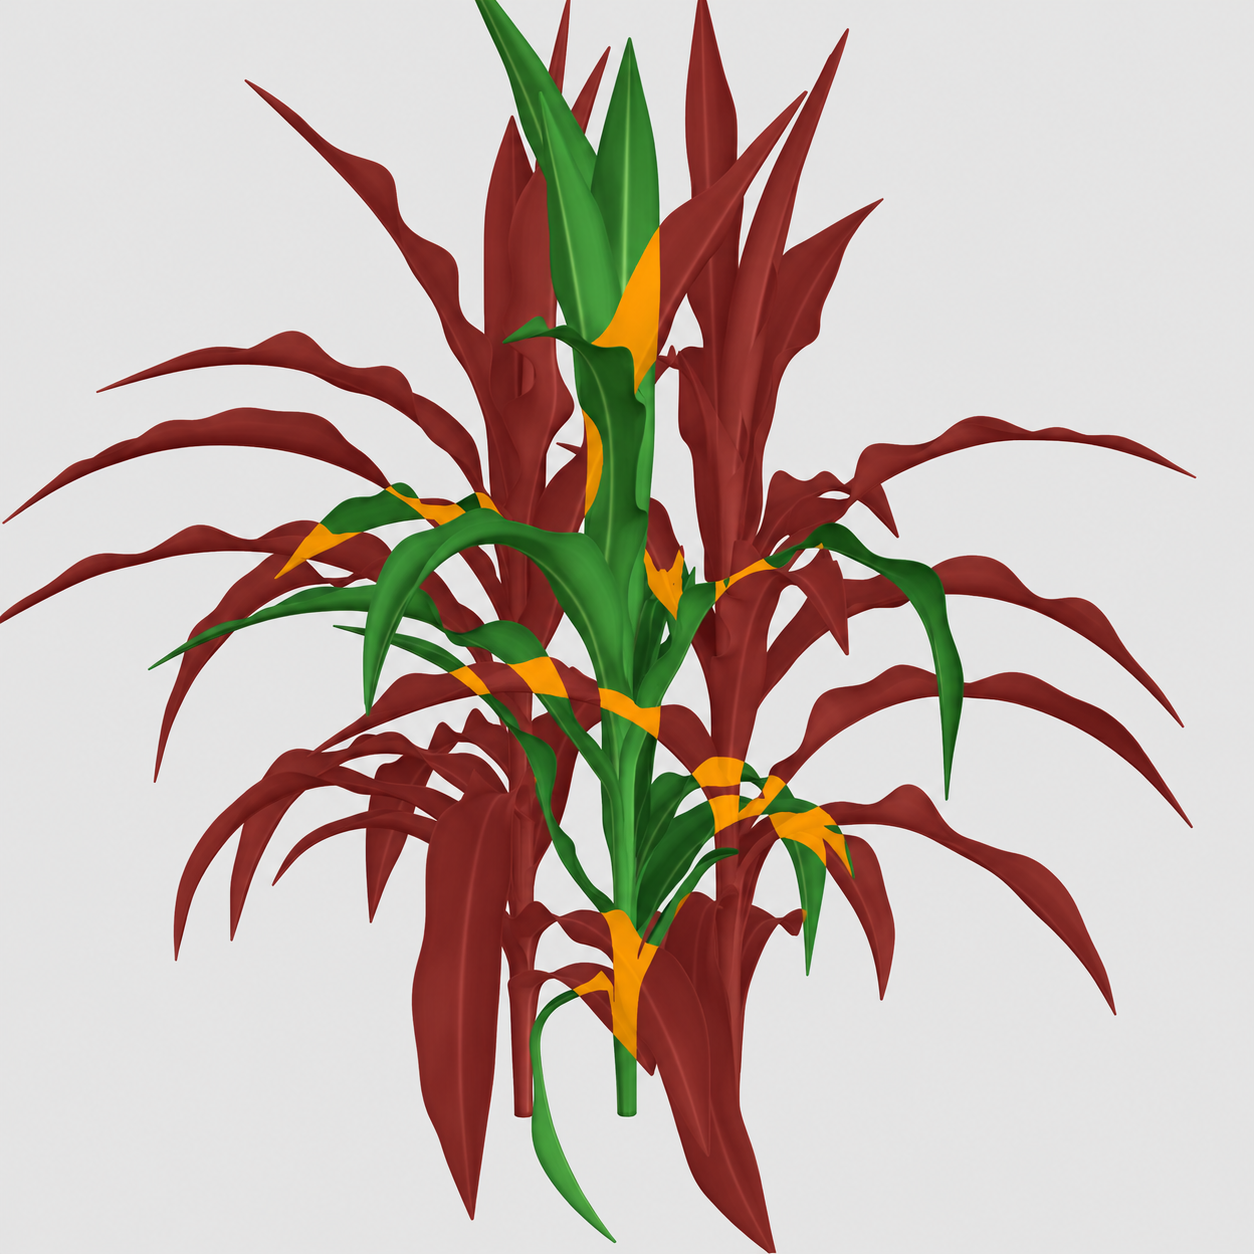
\includegraphics[width=0.7000in, height=0.7000in]{Figures/fig3/sorghum_row_image.png}};
\node[anchor=north, inner sep=0, text=c111111, rotate=0, font={\fontsize{5.6}{6.7}\selectfont\sffamily}] at (3.3700,0.1000) {16 \% hidden};
\draw[draw=cD091A7, line width=1.00pt, rounded corners=3.60pt, fill=cF6E9ED] (3.7700,0.1300) rectangle (4.5300,0.8900);
\node[anchor=south west, inner sep=0] at (3.8000,0.1600) {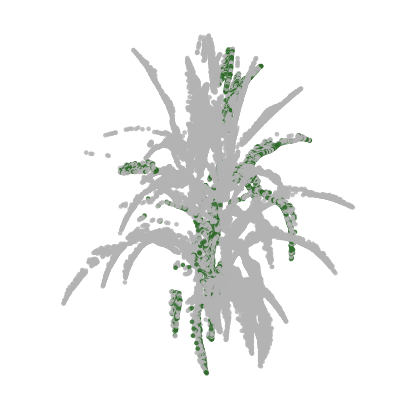
\includegraphics[width=0.7000in, height=0.7000in]{Figures/fig3/sorghum_row_cloud.png}};
\node[anchor=north, inner sep=0, text=c111111, rotate=0, font={\fontsize{5.6}{6.7}\selectfont\sffamily}] at (4.1500,0.1000) {89 \% neighbors};
\node[anchor=base, inner sep=0, text=c111111, rotate=0, font={\fontsize{6.2}{7.4}\selectfont\sffamily\bfseries}] at (5.5400,0.9350) {Maize};
\draw[draw=c809EC2, line width=1.00pt, rounded corners=3.60pt, fill=cE6ECF3] (4.7700,0.1300) rectangle (5.5300,0.8900);
\node[anchor=south west, inner sep=0] at (4.8000,0.1600) {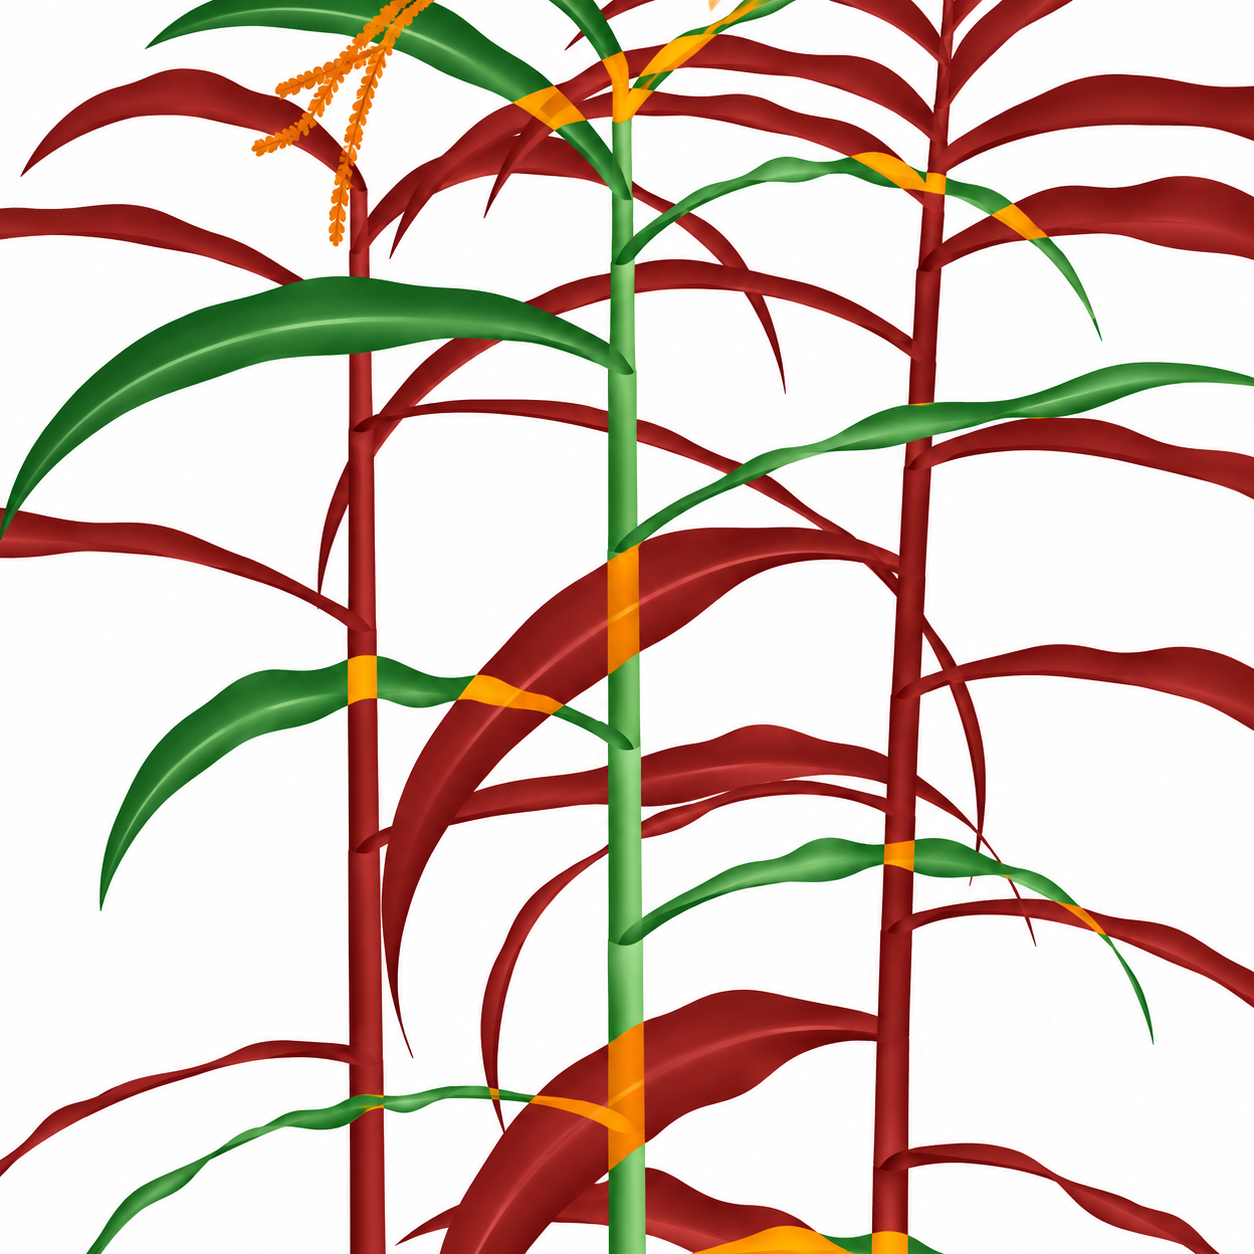
\includegraphics[width=0.7000in, height=0.7000in]{Figures/fig3/maize_row_image.png}};
\node[anchor=north, inner sep=0, text=c111111, rotate=0, font={\fontsize{5.6}{6.7}\selectfont\sffamily}] at (5.1500,0.1000) {15 \% hidden};
\draw[draw=cD091A7, line width=1.00pt, rounded corners=3.60pt, fill=cF6E9ED] (5.5500,0.1300) rectangle (6.3100,0.8900);
\node[anchor=south west, inner sep=0] at (5.5800,0.1600) {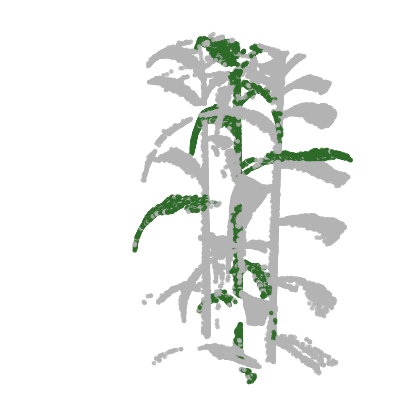
\includegraphics[width=0.7000in, height=0.7000in]{Figures/fig3/maize_row_cloud.png}};
\node[anchor=north, inner sep=0, text=c111111, rotate=0, font={\fontsize{5.6}{6.7}\selectfont\sffamily}] at (5.9300,0.1000) {75 \% neighbors};
\end{tikzpicture}
}.
\definecolor{c111111}{HTML}{111111}%
\definecolor{c333333}{HTML}{333333}%
\definecolor{c3F5F8F}{HTML}{3F5F8F}%
\definecolor{c444444}{HTML}{444444}%
\definecolor{c555555}{HTML}{555555}%
\definecolor{c5E4A96}{HTML}{5E4A96}%
\definecolor{c809EC2}{HTML}{809EC2}%
\definecolor{c9A9A9A}{HTML}{9A9A9A}%
\definecolor{c9D8CC4}{HTML}{9D8CC4}%
\definecolor{cA07800}{HTML}{A07800}%
\definecolor{cA8456E}{HTML}{A8456E}%
\definecolor{cD091A7}{HTML}{D091A7}%
\definecolor{cE0B020}{HTML}{E0B020}%
\definecolor{cE6ECF3}{HTML}{E6ECF3}%
\definecolor{cEAE7F2}{HTML}{EAE7F2}%
\definecolor{cF4F4F5}{HTML}{F4F4F5}%
\definecolor{cF6E9ED}{HTML}{F6E9ED}%
\definecolor{cFAF2D4}{HTML}{FAF2D4}%
\begin{tikzpicture}[x=1in, y=1in]
\useasboundingbox (0,0) rectangle (6.875,3.86);
\node[anchor=base west, inner sep=0, text=c111111, rotate=0, font={\fontsize{9.0}{10.8}\selectfont\sffamily\bfseries}] at (0.0200,3.7200) {a};
\node[anchor=base west, inner sep=0, text=c111111, rotate=0, font={\fontsize{6.2}{7.4}\selectfont\sffamily}] at (0.1800,3.7200) {The plants: \textbf{15,000} per species.};
\node[anchor=base west, inner sep=0, text=c111111, rotate=0, font={\fontsize{9.0}{10.8}\selectfont\sffamily\bfseries}] at (2.3800,3.7200) {b};
\node[anchor=base west, inner sep=0, text=c111111, rotate=0, font={\fontsize{6.2}{7.4}\selectfont\sffamily}] at (2.5400,3.7200) {One view of the boxed plant as its four streams};
\draw[draw=c809EC2, line width=1.00pt, rounded corners=4.32pt, fill=cE6ECF3] (0.2400,2.4100) rectangle (1.7500,3.4450);
\node[anchor=center, inner sep=0, text=c111111, rotate=90, font={\fontsize{7.0}{8.4}\selectfont\sffamily\bfseries}] at (0.1500,2.9275) {Sorghum};
\node[anchor=south west, inner sep=0] at (0.3000,2.9450) {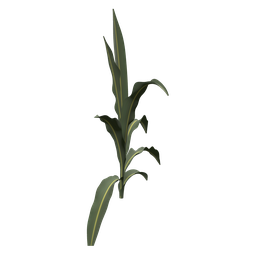
\includegraphics[width=0.4400in, height=0.4400in]{Figures/fig3/sorghum_gallery_0.png}};
\node[anchor=south west, inner sep=0] at (0.7750,2.9450) {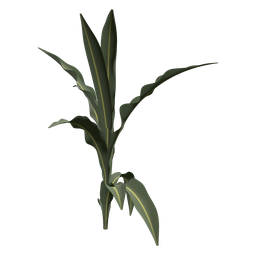
\includegraphics[width=0.4400in, height=0.4400in]{Figures/fig3/sorghum_gallery_1.png}};
\node[anchor=south west, inner sep=0] at (1.2500,2.9450) {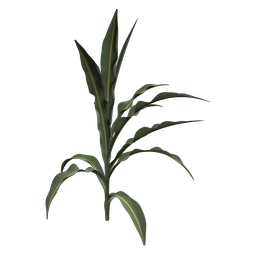
\includegraphics[width=0.4400in, height=0.4400in]{Figures/fig3/sorghum_gallery_2.png}};
\node[anchor=south west, inner sep=0] at (0.3000,2.4700) {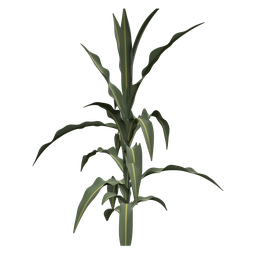
\includegraphics[width=0.4400in, height=0.4400in]{Figures/fig3/sorghum_gallery_3.png}};
\node[anchor=south west, inner sep=0] at (0.7750,2.4700) {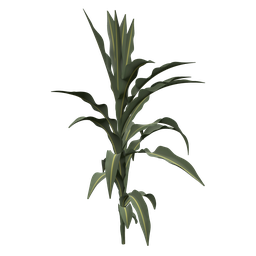
\includegraphics[width=0.4400in, height=0.4400in]{Figures/fig3/sorghum_gallery_4.png}};
\node[anchor=south west, inner sep=0] at (1.2500,2.4700) {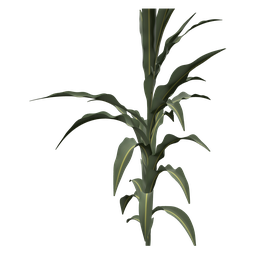
\includegraphics[width=0.4400in, height=0.4400in]{Figures/fig3/sorghum_gallery_5.png}};
\draw[draw=c333333, line width=1.00pt, rounded corners=2.16pt] (1.2350,2.4550) rectangle (1.7050,2.9250);
\draw[draw=c9A9A9A, line width=0.60pt] (1.7050,2.9250) -- (2.3700,3.4175);
\draw[draw=c9A9A9A, line width=0.60pt] (1.7050,2.4550) -- (2.3700,2.4375);
\draw[draw=c9A9A9A, line width=1.00pt, rounded corners=4.32pt, fill=cF4F4F5] (2.3700,2.4375) rectangle (6.8050,3.4175);
\draw[draw=c809EC2, line width=1.00pt, rounded corners=3.60pt, fill=cE6ECF3] (2.4100,2.4775) rectangle (3.3100,3.3775);
\node[anchor=south west, inner sep=0] at (2.4400,2.5075) {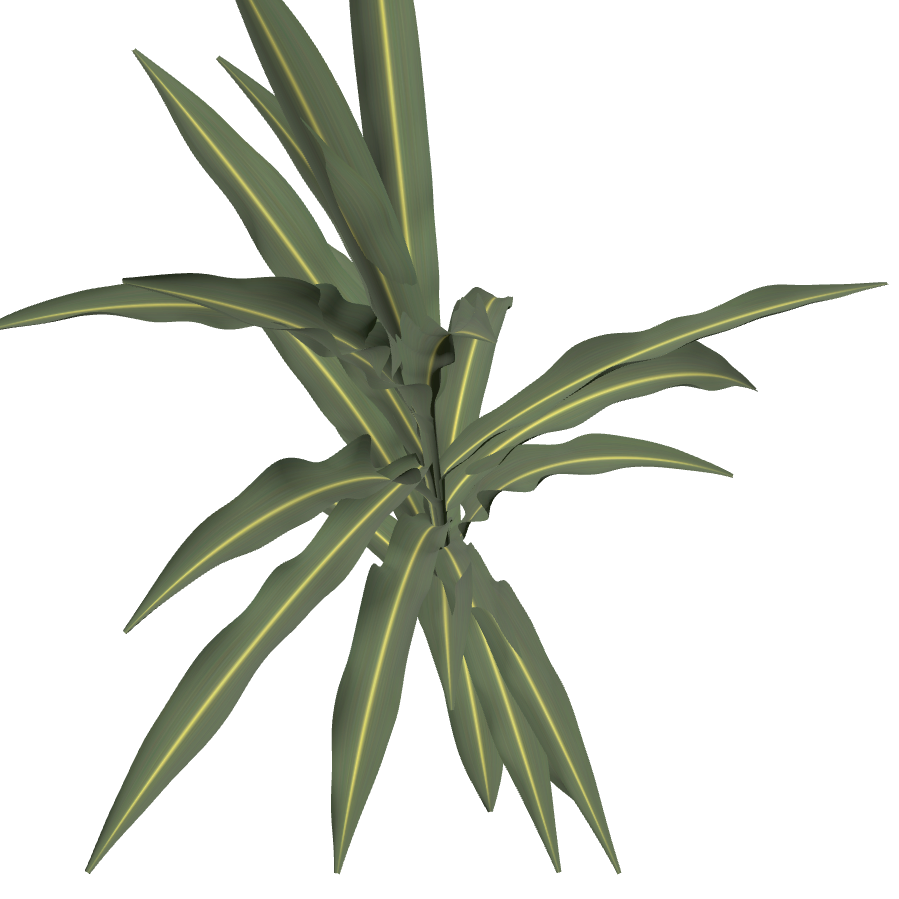
\includegraphics[width=0.8400in, height=0.8400in]{Figures/fig3/sorghum_rgb.png}};
\node[anchor=base, inner sep=0, text=c3F5F8F, rotate=0, font={\fontsize{6.2}{7.4}\selectfont\sffamily\bfseries}] at (2.8600,3.4925) {Image};
\draw[draw=cE0B020, line width=1.00pt, rounded corners=3.60pt, fill=cFAF2D4] (3.5617,2.4775) rectangle (4.4617,3.3775);
\node[anchor=south west, inner sep=0] at (3.5917,2.5075) {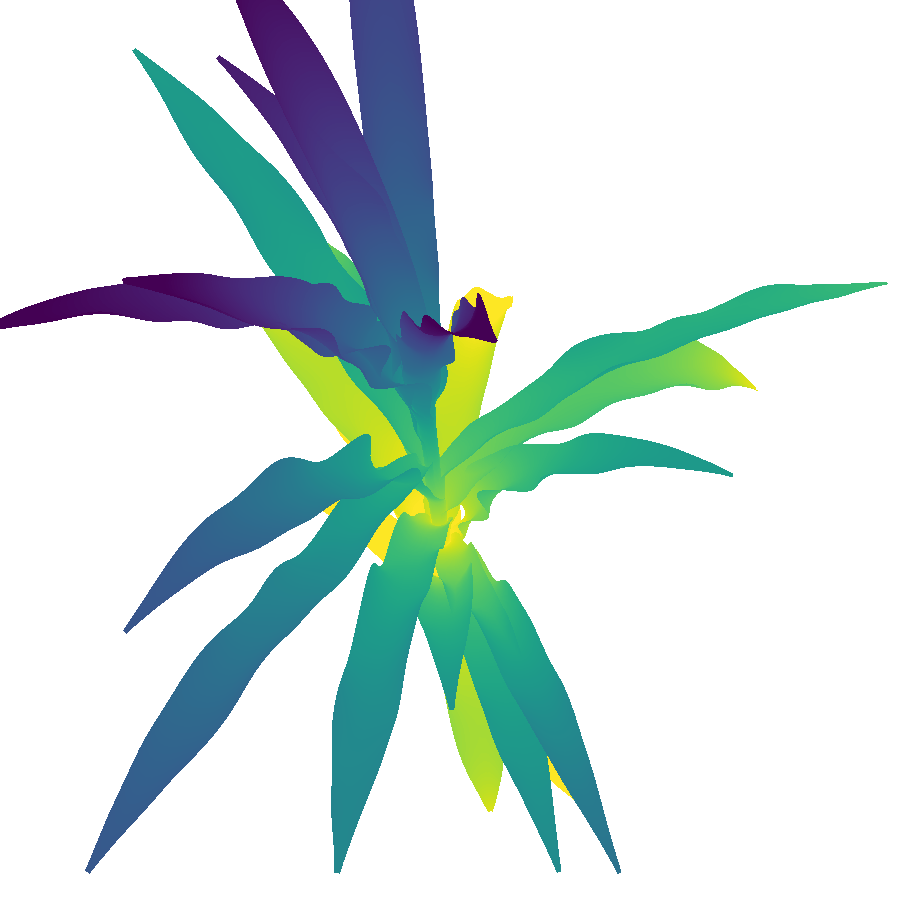
\includegraphics[width=0.8400in, height=0.8400in]{Figures/fig3/sorghum_depth.png}};
\node[anchor=base, inner sep=0, text=cA07800, rotate=0, font={\fontsize{6.2}{7.4}\selectfont\sffamily\bfseries}] at (4.0117,3.4925) {Depth image};
\draw[draw=cD091A7, line width=1.00pt, rounded corners=3.60pt, fill=cF6E9ED] (4.7133,2.4775) rectangle (5.6133,3.3775);
\node[anchor=south west, inner sep=0] at (4.7433,2.5075) {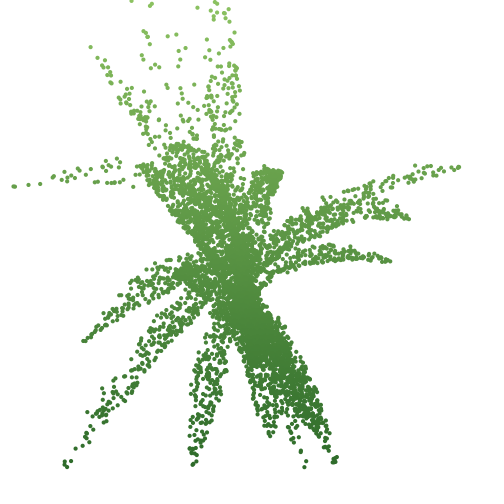
\includegraphics[width=0.8400in, height=0.8400in]{Figures/fig3/sorghum_pc.png}};
\node[anchor=base, inner sep=0, text=cA8456E, rotate=0, font={\fontsize{6.2}{7.4}\selectfont\sffamily\bfseries}] at (5.1633,3.4925) {Point Cloud};
\draw[draw=c9D8CC4, line width=1.00pt, rounded corners=3.60pt, fill=cEAE7F2] (5.8650,2.4775) rectangle (6.7650,3.3775);
\node[anchor=south west, inner sep=0] at (5.8950,2.5075) {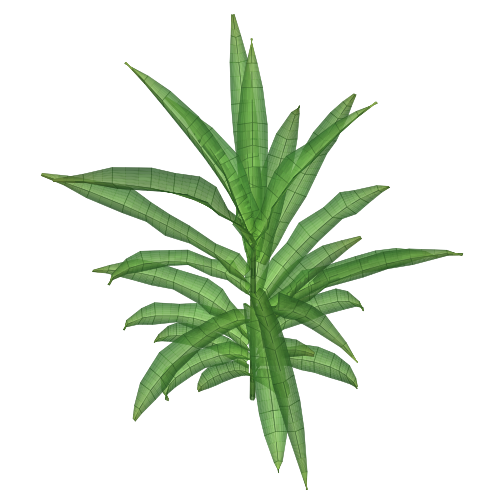
\includegraphics[width=0.8400in, height=0.8400in]{Figures/fig3/sorghum_text.png}};
\node[anchor=base, inner sep=0, text=c5E4A96, rotate=0, font={\fontsize{6.2}{7.4}\selectfont\sffamily\bfseries}] at (6.3150,3.4925) {Procedural Model};
\draw[draw=c809EC2, line width=1.00pt, rounded corners=4.32pt, fill=cE6ECF3] (0.2400,1.3100) rectangle (1.7500,2.3450);
\node[anchor=center, inner sep=0, text=c111111, rotate=90, font={\fontsize{7.0}{8.4}\selectfont\sffamily\bfseries}] at (0.1500,1.8275) {Maize};
\node[anchor=south west, inner sep=0] at (0.3000,1.8450) {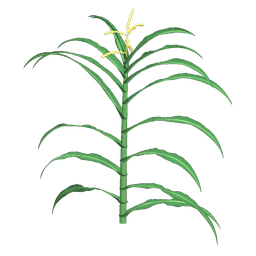
\includegraphics[width=0.4400in, height=0.4400in]{Figures/fig3/maize_gallery_0.png}};
\node[anchor=south west, inner sep=0] at (0.7750,1.8450) {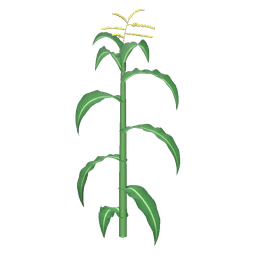
\includegraphics[width=0.4400in, height=0.4400in]{Figures/fig3/maize_gallery_1.png}};
\node[anchor=south west, inner sep=0] at (1.2500,1.8450) {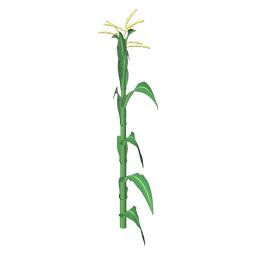
\includegraphics[width=0.4400in, height=0.4400in]{Figures/fig3/maize_gallery_2.png}};
\node[anchor=south west, inner sep=0] at (0.3000,1.3700) {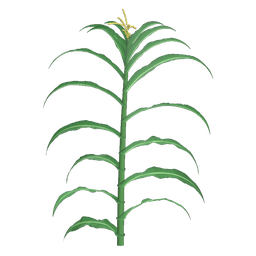
\includegraphics[width=0.4400in, height=0.4400in]{Figures/fig3/maize_gallery_3.png}};
\node[anchor=south west, inner sep=0] at (0.7750,1.3700) {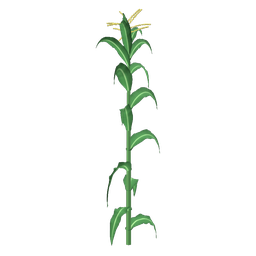
\includegraphics[width=0.4400in, height=0.4400in]{Figures/fig3/maize_gallery_4.png}};
\node[anchor=south west, inner sep=0] at (1.2500,1.3700) {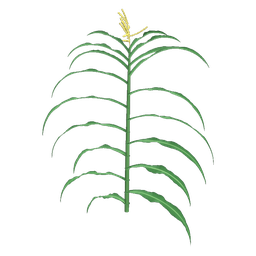
\includegraphics[width=0.4400in, height=0.4400in]{Figures/fig3/maize_gallery_5.png}};
\draw[draw=c333333, line width=1.00pt, rounded corners=2.16pt] (1.2350,1.3550) rectangle (1.7050,1.8250);
\draw[draw=c9A9A9A, line width=0.60pt] (1.7050,1.8250) -- (2.3700,2.3175);
\draw[draw=c9A9A9A, line width=0.60pt] (1.7050,1.3550) -- (2.3700,1.3375);
\draw[draw=c9A9A9A, line width=1.00pt, rounded corners=4.32pt, fill=cF4F4F5] (2.3700,1.3375) rectangle (6.8050,2.3175);
\draw[draw=c809EC2, line width=1.00pt, rounded corners=3.60pt, fill=cE6ECF3] (2.4100,1.3775) rectangle (3.3100,2.2775);
\node[anchor=south west, inner sep=0] at (2.4400,1.4075) {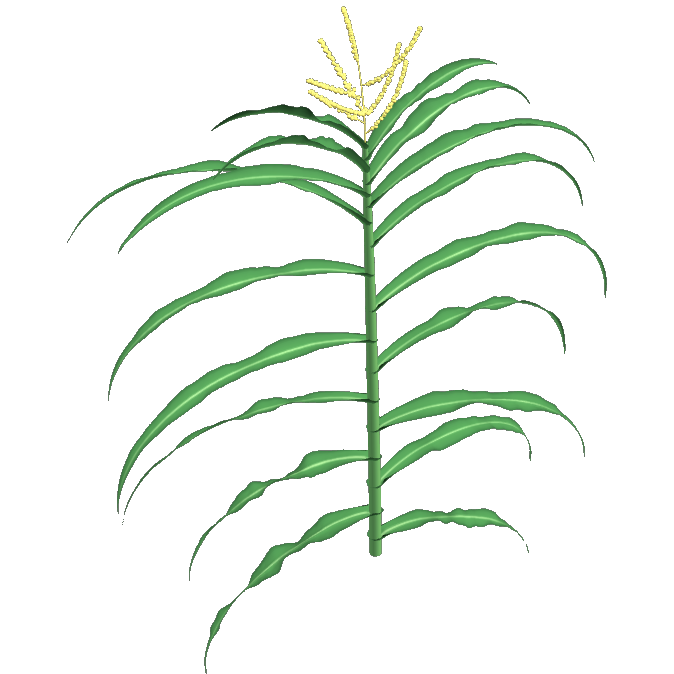
\includegraphics[width=0.8400in, height=0.8400in]{Figures/fig3/maize_rgb.png}};
\draw[draw=cE0B020, line width=1.00pt, rounded corners=3.60pt, fill=cFAF2D4] (3.5617,1.3775) rectangle (4.4617,2.2775);
\node[anchor=south west, inner sep=0] at (3.5917,1.4075) {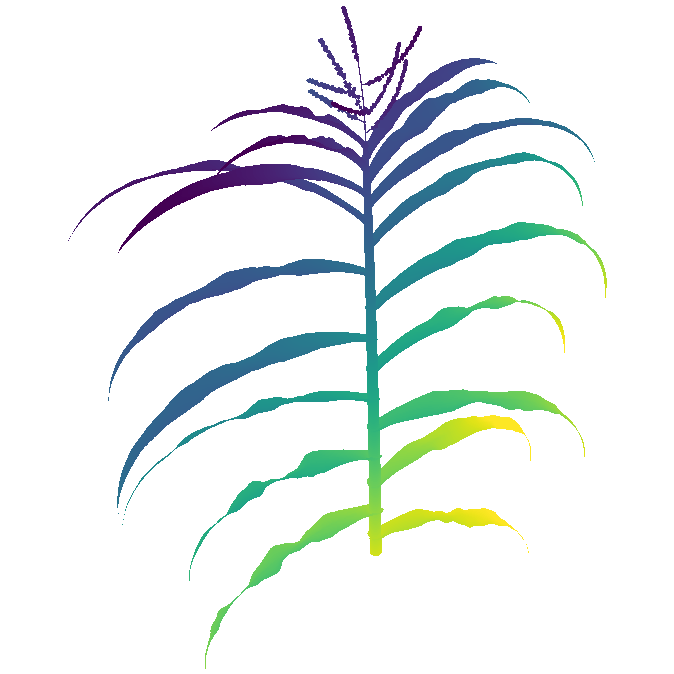
\includegraphics[width=0.8400in, height=0.8400in]{Figures/fig3/maize_depth.png}};
\draw[draw=cD091A7, line width=1.00pt, rounded corners=3.60pt, fill=cF6E9ED] (4.7133,1.3775) rectangle (5.6133,2.2775);
\node[anchor=south west, inner sep=0] at (4.7433,1.4075) {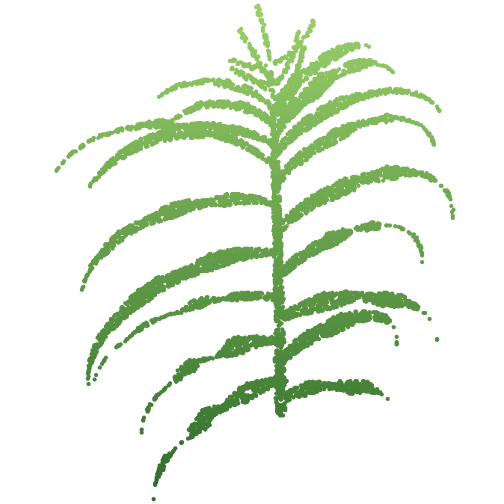
\includegraphics[width=0.8400in, height=0.8400in]{Figures/fig3/maize_pc.png}};
\draw[draw=c9D8CC4, line width=1.00pt, rounded corners=3.60pt, fill=cEAE7F2] (5.8650,1.3775) rectangle (6.7650,2.2775);
\node[anchor=south west, inner sep=0] at (5.8950,1.4075) {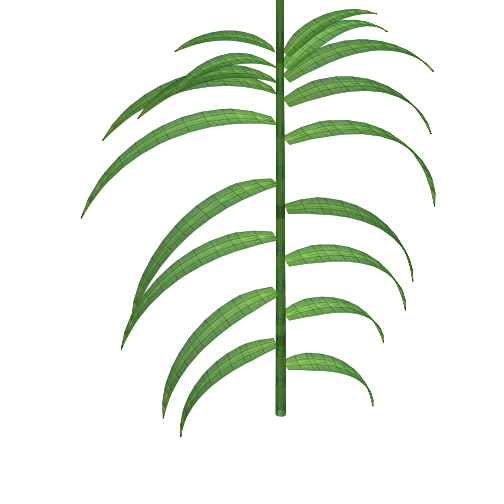
\includegraphics[width=0.8400in, height=0.8400in]{Figures/fig3/maize_text.png}};
\node[anchor=base west, inner sep=0, text=c111111, rotate=0, font={\fontsize{9.0}{10.8}\selectfont\sffamily\bfseries}] at (0.0200,1.1300) {c};
\node[anchor=base west, inner sep=0, text=c111111, rotate=0, font={\fontsize{6.2}{7.4}\selectfont\sffamily}] at (0.1800,1.1300) {Ten cameras per plant (five shown), by elevation};
\draw[draw=c809EC2, line width=1.00pt, rounded corners=2.88pt, fill=cE6ECF3] (0.2600,0.5600) rectangle (2.1800,0.9800);
\node[anchor=center, inner sep=0, text=c111111, rotate=90, font={\fontsize{5.8}{7.0}\selectfont\sffamily\bfseries}] at (0.1500,0.7700) {Sorghum};
\node[anchor=south west, inner sep=0] at (0.3000,0.6000) {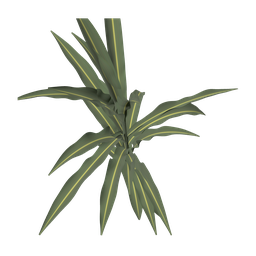
\includegraphics[width=0.3400in, height=0.3400in]{Figures/fig3/sorghum_camera_0.png}};
\node[anchor=south, inner sep=0, text=c444444, rotate=0, font={\fontsize{5.4}{6.5}\selectfont\sffamily}] at (0.4700,0.9900) {+64$^{\circ}$};
\node[anchor=south west, inner sep=0] at (0.6750,0.6000) {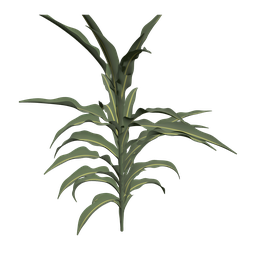
\includegraphics[width=0.3400in, height=0.3400in]{Figures/fig3/sorghum_camera_1.png}};
\node[anchor=south, inner sep=0, text=c444444, rotate=0, font={\fontsize{5.4}{6.5}\selectfont\sffamily}] at (0.8450,0.9900) {+30$^{\circ}$};
\node[anchor=south west, inner sep=0] at (1.0500,0.6000) {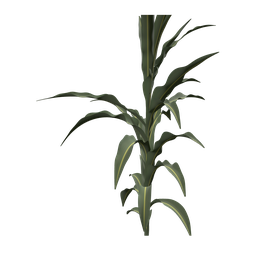
\includegraphics[width=0.3400in, height=0.3400in]{Figures/fig3/sorghum_camera_2.png}};
\node[anchor=south, inner sep=0, text=c444444, rotate=0, font={\fontsize{5.4}{6.5}\selectfont\sffamily}] at (1.2200,0.9900) {+6$^{\circ}$};
\node[anchor=south west, inner sep=0] at (1.4250,0.6000) {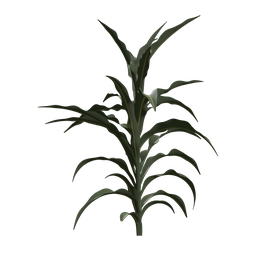
\includegraphics[width=0.3400in, height=0.3400in]{Figures/fig3/sorghum_camera_3.png}};
\node[anchor=south, inner sep=0, text=c444444, rotate=0, font={\fontsize{5.4}{6.5}\selectfont\sffamily}] at (1.5950,0.9900) {$-$17$^{\circ}$};
\node[anchor=south west, inner sep=0] at (1.8000,0.6000) {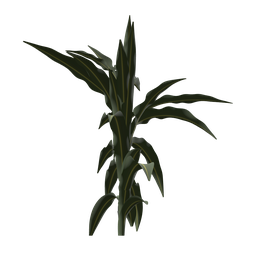
\includegraphics[width=0.3400in, height=0.3400in]{Figures/fig3/sorghum_camera_4.png}};
\node[anchor=south, inner sep=0, text=c444444, rotate=0, font={\fontsize{5.4}{6.5}\selectfont\sffamily}] at (1.9700,0.9900) {$-$44$^{\circ}$};
\draw[draw=c809EC2, line width=1.00pt, rounded corners=2.88pt, fill=cE6ECF3] (0.2600,0.0300) rectangle (2.1800,0.4500);
\node[anchor=center, inner sep=0, text=c111111, rotate=90, font={\fontsize{5.8}{7.0}\selectfont\sffamily\bfseries}] at (0.1500,0.2400) {Maize};
\node[anchor=south west, inner sep=0] at (0.3000,0.0700) {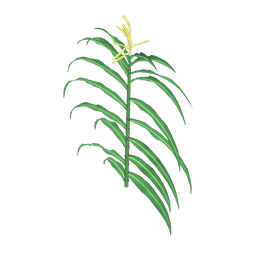
\includegraphics[width=0.3400in, height=0.3400in]{Figures/fig3/maize_camera_0.png}};
\node[anchor=south, inner sep=0, text=c444444, rotate=0, font={\fontsize{5.4}{6.5}\selectfont\sffamily}] at (0.4700,0.4600) {+39$^{\circ}$};
\node[anchor=south west, inner sep=0] at (0.6750,0.0700) {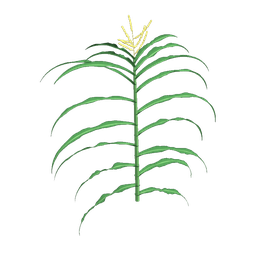
\includegraphics[width=0.3400in, height=0.3400in]{Figures/fig3/maize_camera_1.png}};
\node[anchor=south, inner sep=0, text=c444444, rotate=0, font={\fontsize{5.4}{6.5}\selectfont\sffamily}] at (0.8450,0.4600) {+30$^{\circ}$};
\node[anchor=south west, inner sep=0] at (1.0500,0.0700) {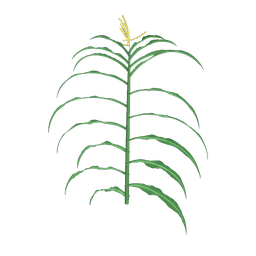
\includegraphics[width=0.3400in, height=0.3400in]{Figures/fig3/maize_camera_2.png}};
\node[anchor=south, inner sep=0, text=c444444, rotate=0, font={\fontsize{5.4}{6.5}\selectfont\sffamily}] at (1.2200,0.4600) {+10$^{\circ}$};
\node[anchor=south west, inner sep=0] at (1.4250,0.0700) {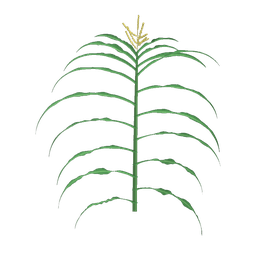
\includegraphics[width=0.3400in, height=0.3400in]{Figures/fig3/maize_camera_3.png}};
\node[anchor=south, inner sep=0, text=c444444, rotate=0, font={\fontsize{5.4}{6.5}\selectfont\sffamily}] at (1.5950,0.4600) {$-$13$^{\circ}$};
\node[anchor=south west, inner sep=0] at (1.8000,0.0700) {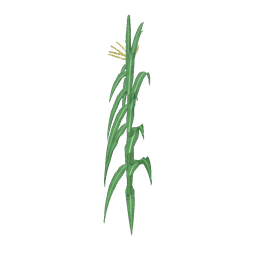
\includegraphics[width=0.3400in, height=0.3400in]{Figures/fig3/maize_camera_4.png}};
\node[anchor=south, inner sep=0, text=c444444, rotate=0, font={\fontsize{5.4}{6.5}\selectfont\sffamily}] at (1.9700,0.4600) {$-$36$^{\circ}$};
\node[anchor=base west, inner sep=0, text=c111111, rotate=0, font={\fontsize{9.0}{10.8}\selectfont\sffamily\bfseries}] at (2.8400,1.1300) {d};
\node[anchor=base west, inner sep=0, text=c111111, rotate=0, font={\fontsize{6.2}{7.4}\selectfont\sffamily}] at (3.0000,1.1300) {Crop rows: the target plant between neighbors};
\node[anchor=base west, inner sep=0, text=c555555, rotate=0, font={\fontsize{5.4}{6.5}\selectfont\sffamily}] at (3.0000,1.0250) {\textcolor{cLegRed}{\textbf{Red}}: Neighbor pixels  \textcolor{cLegOrange}{\textbf{Orange}}: Target pixels occluded by neighbors (\% hidden)  \textcolor{cLegGreen}{\textbf{Green}}: Target points};
\node[anchor=base, inner sep=0, text=c111111, rotate=0, font={\fontsize{6.2}{7.4}\selectfont\sffamily\bfseries}] at (3.7600,0.9350) {Sorghum};
\draw[draw=c809EC2, line width=1.00pt, rounded corners=3.60pt, fill=cE6ECF3] (2.9900,0.1300) rectangle (3.7500,0.8900);
\node[anchor=south west, inner sep=0] at (3.0200,0.1600) {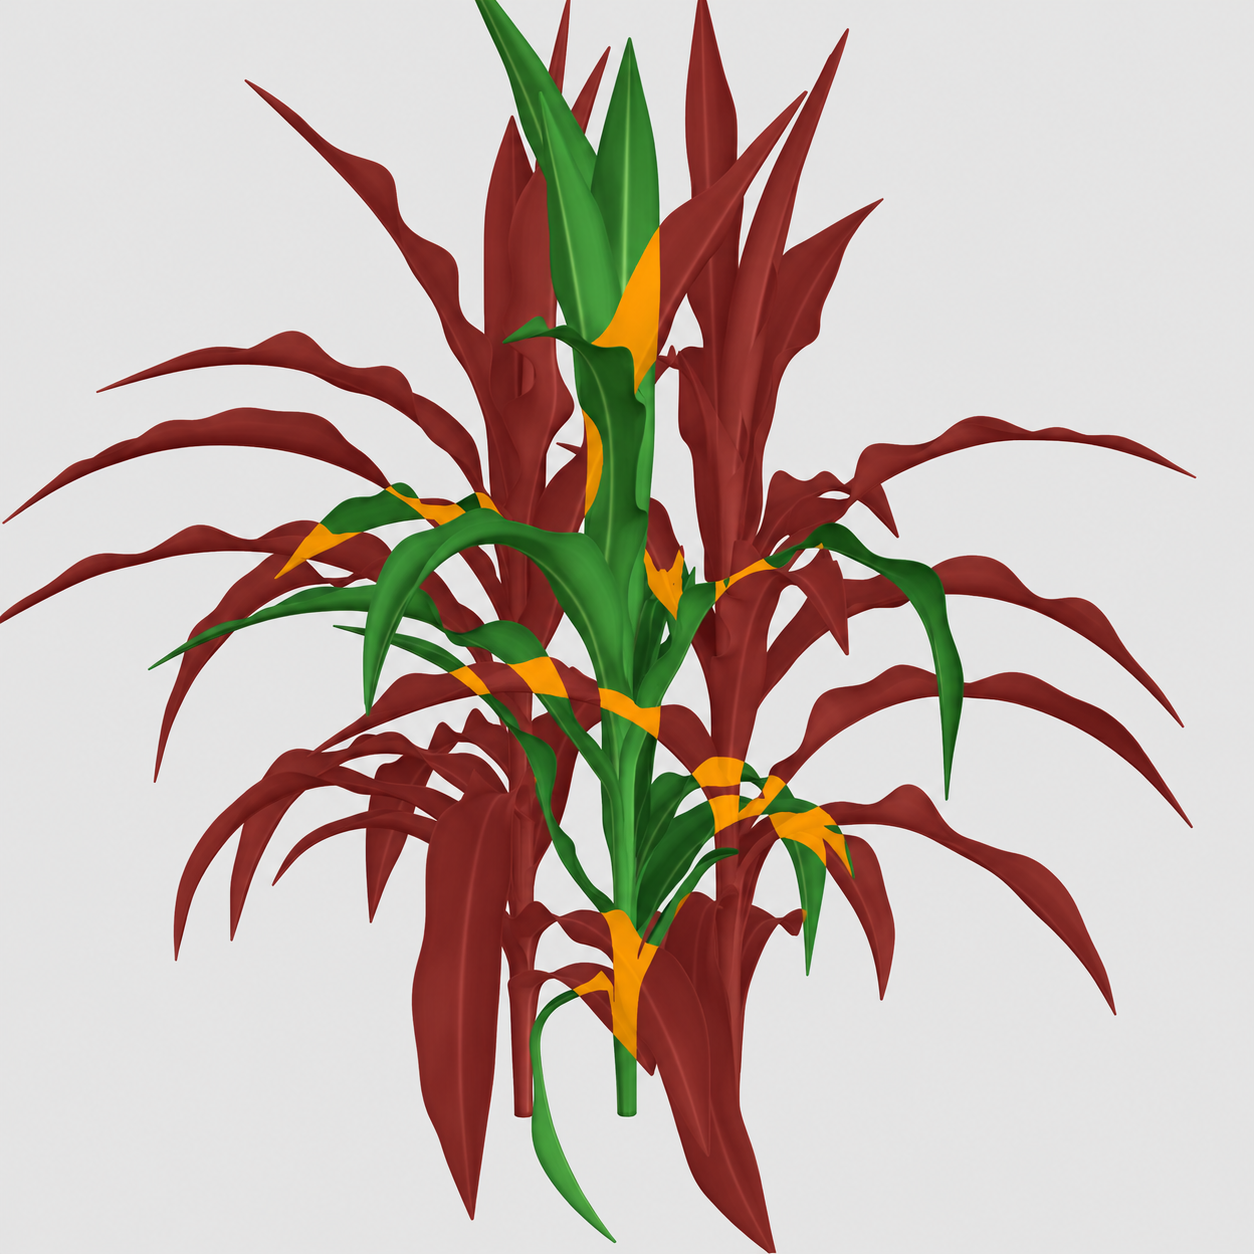
\includegraphics[width=0.7000in, height=0.7000in]{Figures/fig3/sorghum_row_image.png}};
\node[anchor=north, inner sep=0, text=c111111, rotate=0, font={\fontsize{5.6}{6.7}\selectfont\sffamily}] at (3.3700,0.1000) {16 \% hidden};
\draw[draw=cD091A7, line width=1.00pt, rounded corners=3.60pt, fill=cF6E9ED] (3.7700,0.1300) rectangle (4.5300,0.8900);
\node[anchor=south west, inner sep=0] at (3.8000,0.1600) {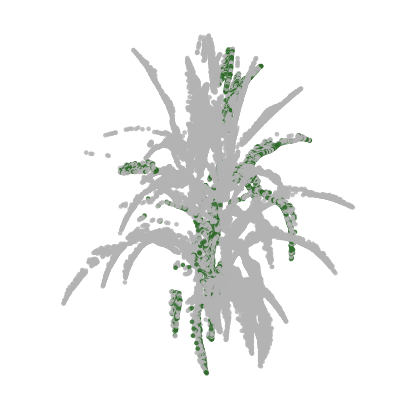
\includegraphics[width=0.7000in, height=0.7000in]{Figures/fig3/sorghum_row_cloud.png}};
\node[anchor=north, inner sep=0, text=c111111, rotate=0, font={\fontsize{5.6}{6.7}\selectfont\sffamily}] at (4.1500,0.1000) {89 \% neighbors};
\node[anchor=base, inner sep=0, text=c111111, rotate=0, font={\fontsize{6.2}{7.4}\selectfont\sffamily\bfseries}] at (5.5400,0.9350) {Maize};
\draw[draw=c809EC2, line width=1.00pt, rounded corners=3.60pt, fill=cE6ECF3] (4.7700,0.1300) rectangle (5.5300,0.8900);
\node[anchor=south west, inner sep=0] at (4.8000,0.1600) {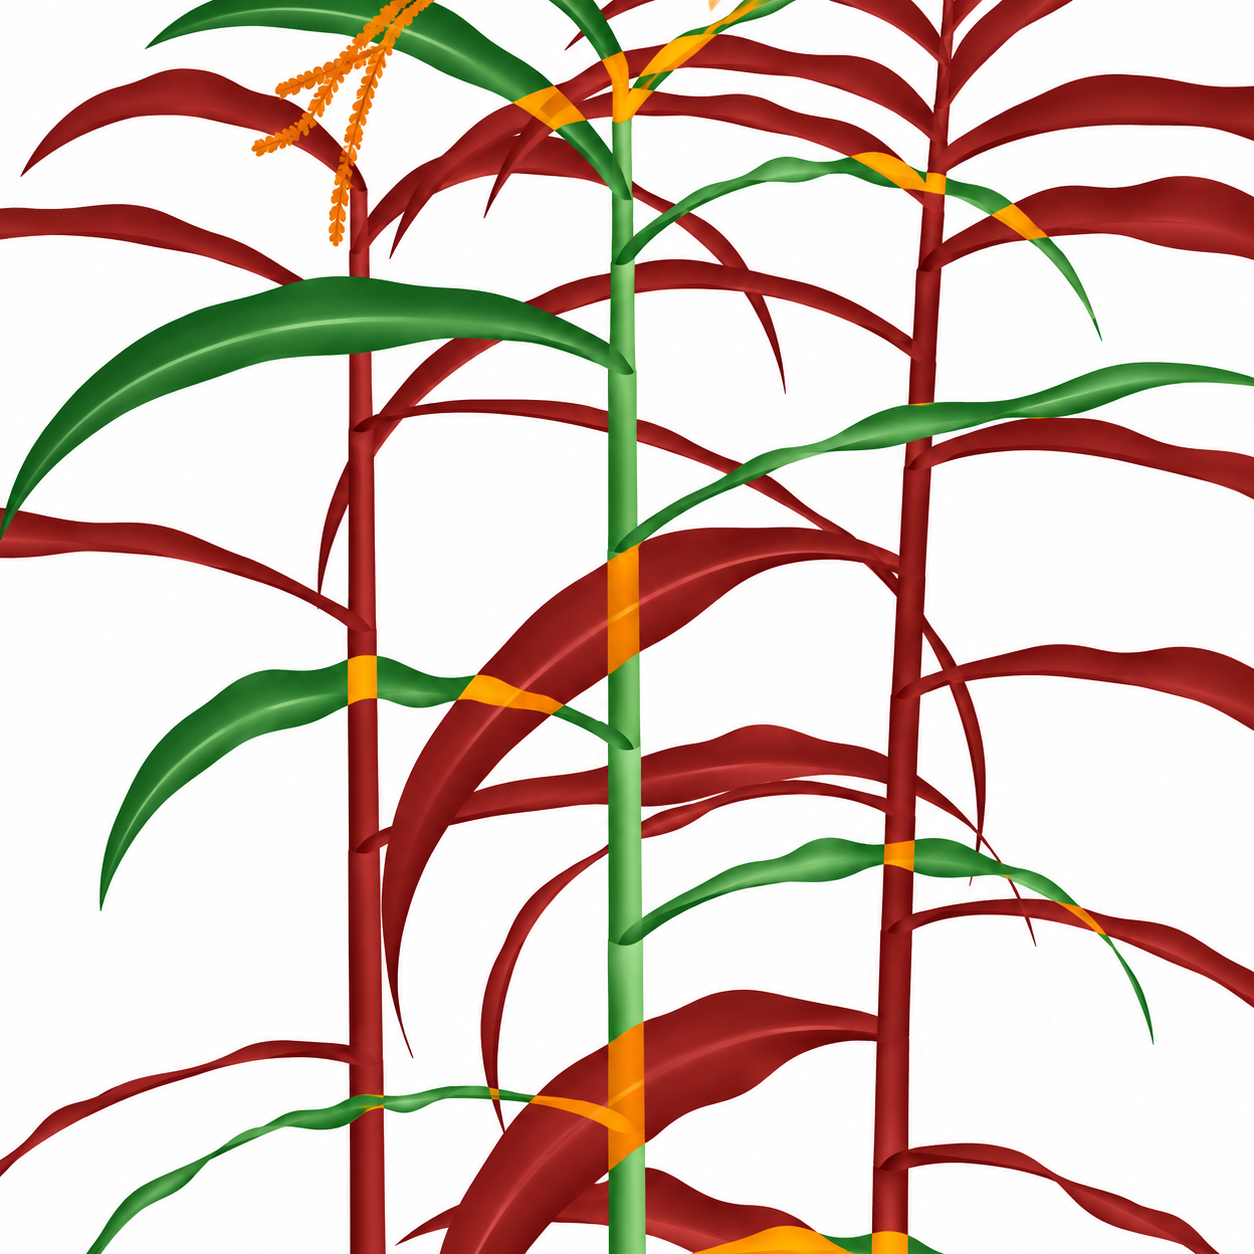
\includegraphics[width=0.7000in, height=0.7000in]{Figures/fig3/maize_row_image.png}};
\node[anchor=north, inner sep=0, text=c111111, rotate=0, font={\fontsize{5.6}{6.7}\selectfont\sffamily}] at (5.1500,0.1000) {15 \% hidden};
\draw[draw=cD091A7, line width=1.00pt, rounded corners=3.60pt, fill=cF6E9ED] (5.5500,0.1300) rectangle (6.3100,0.8900);
\node[anchor=south west, inner sep=0] at (5.5800,0.1600) {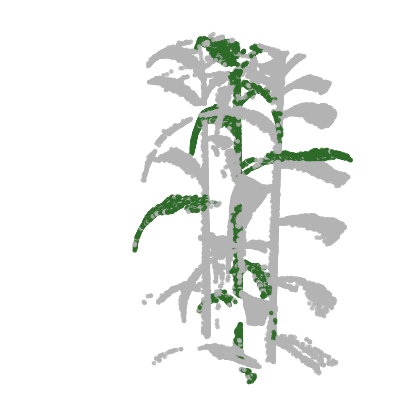
\includegraphics[width=0.7000in, height=0.7000in]{Figures/fig3/maize_row_cloud.png}};
\node[anchor=north, inner sep=0, text=c111111, rotate=0, font={\fontsize{5.6}{6.7}\selectfont\sffamily}] at (5.9300,0.1000) {75 \% neighbors};
\end{tikzpicture}
}.
\definecolor{c111111}{HTML}{111111}%
\definecolor{c333333}{HTML}{333333}%
\definecolor{c3F5F8F}{HTML}{3F5F8F}%
\definecolor{c444444}{HTML}{444444}%
\definecolor{c555555}{HTML}{555555}%
\definecolor{c5E4A96}{HTML}{5E4A96}%
\definecolor{c809EC2}{HTML}{809EC2}%
\definecolor{c9A9A9A}{HTML}{9A9A9A}%
\definecolor{c9D8CC4}{HTML}{9D8CC4}%
\definecolor{cA07800}{HTML}{A07800}%
\definecolor{cA8456E}{HTML}{A8456E}%
\definecolor{cD091A7}{HTML}{D091A7}%
\definecolor{cE0B020}{HTML}{E0B020}%
\definecolor{cE6ECF3}{HTML}{E6ECF3}%
\definecolor{cEAE7F2}{HTML}{EAE7F2}%
\definecolor{cF4F4F5}{HTML}{F4F4F5}%
\definecolor{cF6E9ED}{HTML}{F6E9ED}%
\definecolor{cFAF2D4}{HTML}{FAF2D4}%
\begin{tikzpicture}[x=1in, y=1in]
\useasboundingbox (0,0) rectangle (6.875,3.86);
\node[anchor=base west, inner sep=0, text=c111111, rotate=0, font={\fontsize{9.0}{10.8}\selectfont\sffamily\bfseries}] at (0.0200,3.7200) {a};
\node[anchor=base west, inner sep=0, text=c111111, rotate=0, font={\fontsize{6.2}{7.4}\selectfont\sffamily}] at (0.1800,3.7200) {The plants: \textbf{15,000} per species.};
\node[anchor=base west, inner sep=0, text=c111111, rotate=0, font={\fontsize{9.0}{10.8}\selectfont\sffamily\bfseries}] at (2.3800,3.7200) {b};
\node[anchor=base west, inner sep=0, text=c111111, rotate=0, font={\fontsize{6.2}{7.4}\selectfont\sffamily}] at (2.5400,3.7200) {One view of the boxed plant as its four streams};
\draw[draw=c809EC2, line width=1.00pt, rounded corners=4.32pt, fill=cE6ECF3] (0.2400,2.4100) rectangle (1.7500,3.4450);
\node[anchor=center, inner sep=0, text=c111111, rotate=90, font={\fontsize{7.0}{8.4}\selectfont\sffamily\bfseries}] at (0.1500,2.9275) {Sorghum};
\node[anchor=south west, inner sep=0] at (0.3000,2.9450) {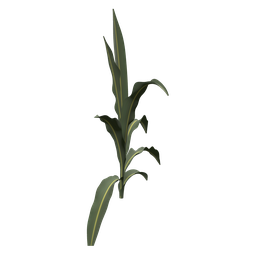
\includegraphics[width=0.4400in, height=0.4400in]{Figures/fig3/sorghum_gallery_0.png}};
\node[anchor=south west, inner sep=0] at (0.7750,2.9450) {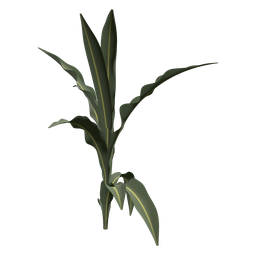
\includegraphics[width=0.4400in, height=0.4400in]{Figures/fig3/sorghum_gallery_1.png}};
\node[anchor=south west, inner sep=0] at (1.2500,2.9450) {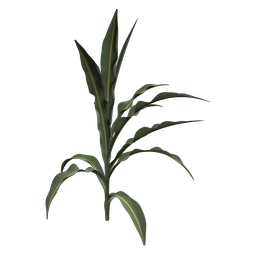
\includegraphics[width=0.4400in, height=0.4400in]{Figures/fig3/sorghum_gallery_2.png}};
\node[anchor=south west, inner sep=0] at (0.3000,2.4700) {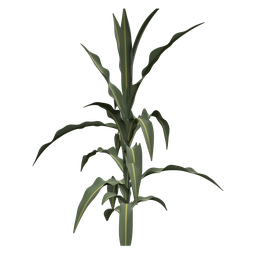
\includegraphics[width=0.4400in, height=0.4400in]{Figures/fig3/sorghum_gallery_3.png}};
\node[anchor=south west, inner sep=0] at (0.7750,2.4700) {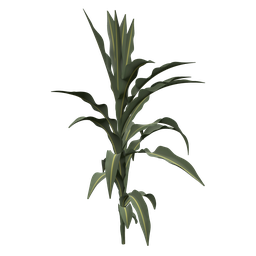
\includegraphics[width=0.4400in, height=0.4400in]{Figures/fig3/sorghum_gallery_4.png}};
\node[anchor=south west, inner sep=0] at (1.2500,2.4700) {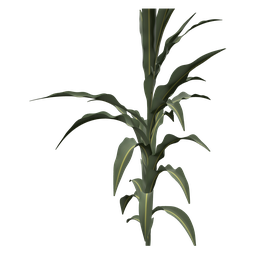
\includegraphics[width=0.4400in, height=0.4400in]{Figures/fig3/sorghum_gallery_5.png}};
\draw[draw=c333333, line width=1.00pt, rounded corners=2.16pt] (1.2350,2.4550) rectangle (1.7050,2.9250);
\draw[draw=c9A9A9A, line width=0.60pt] (1.7050,2.9250) -- (2.3700,3.4175);
\draw[draw=c9A9A9A, line width=0.60pt] (1.7050,2.4550) -- (2.3700,2.4375);
\draw[draw=c9A9A9A, line width=1.00pt, rounded corners=4.32pt, fill=cF4F4F5] (2.3700,2.4375) rectangle (6.8050,3.4175);
\draw[draw=c809EC2, line width=1.00pt, rounded corners=3.60pt, fill=cE6ECF3] (2.4100,2.4775) rectangle (3.3100,3.3775);
\node[anchor=south west, inner sep=0] at (2.4400,2.5075) {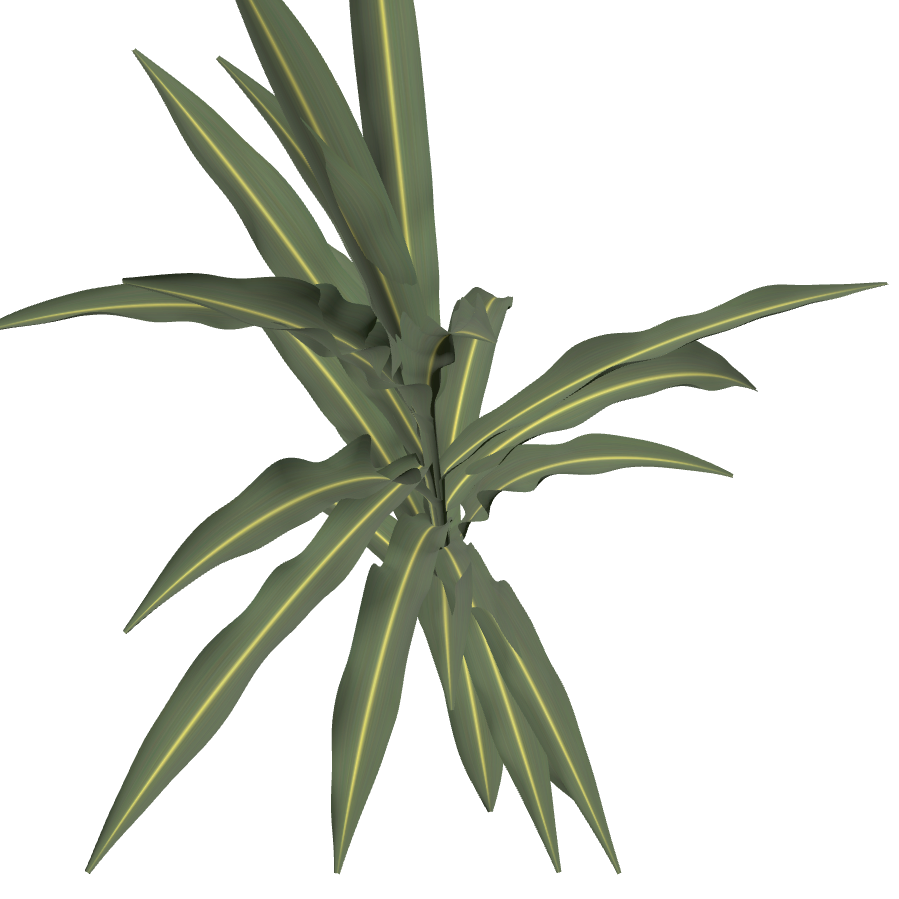
\includegraphics[width=0.8400in, height=0.8400in]{Figures/fig3/sorghum_rgb.png}};
\node[anchor=base, inner sep=0, text=c3F5F8F, rotate=0, font={\fontsize{6.2}{7.4}\selectfont\sffamily\bfseries}] at (2.8600,3.4925) {Image};
\draw[draw=cE0B020, line width=1.00pt, rounded corners=3.60pt, fill=cFAF2D4] (3.5617,2.4775) rectangle (4.4617,3.3775);
\node[anchor=south west, inner sep=0] at (3.5917,2.5075) {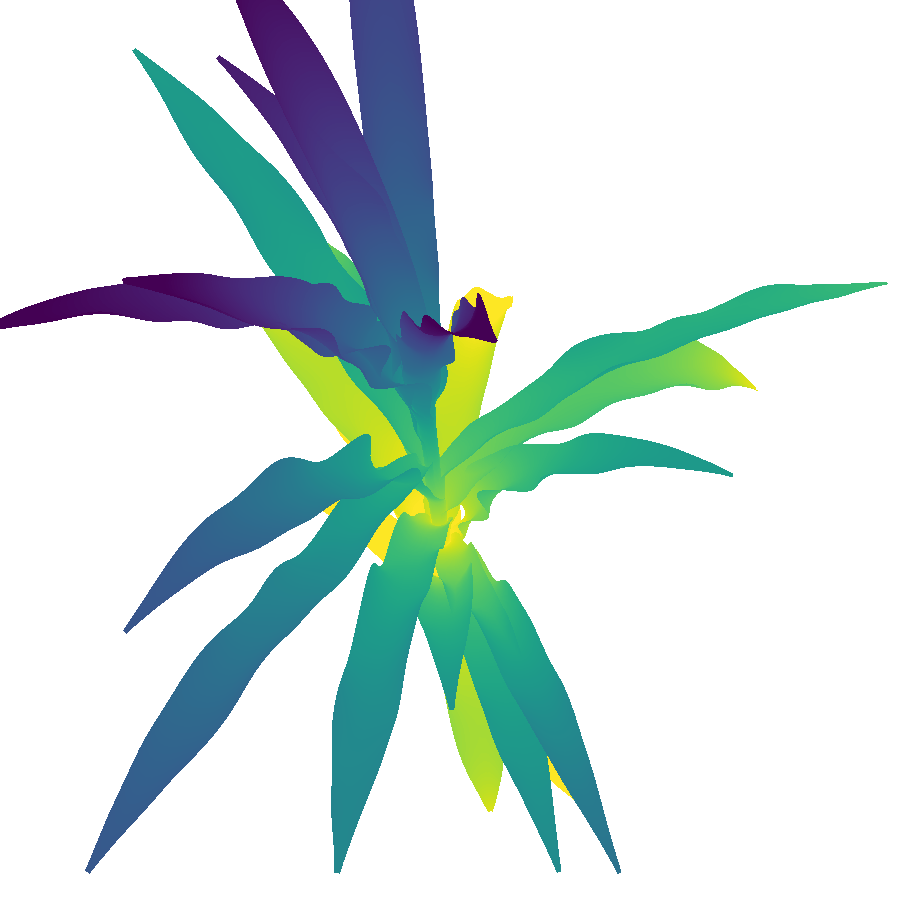
\includegraphics[width=0.8400in, height=0.8400in]{Figures/fig3/sorghum_depth.png}};
\node[anchor=base, inner sep=0, text=cA07800, rotate=0, font={\fontsize{6.2}{7.4}\selectfont\sffamily\bfseries}] at (4.0117,3.4925) {Depth image};
\draw[draw=cD091A7, line width=1.00pt, rounded corners=3.60pt, fill=cF6E9ED] (4.7133,2.4775) rectangle (5.6133,3.3775);
\node[anchor=south west, inner sep=0] at (4.7433,2.5075) {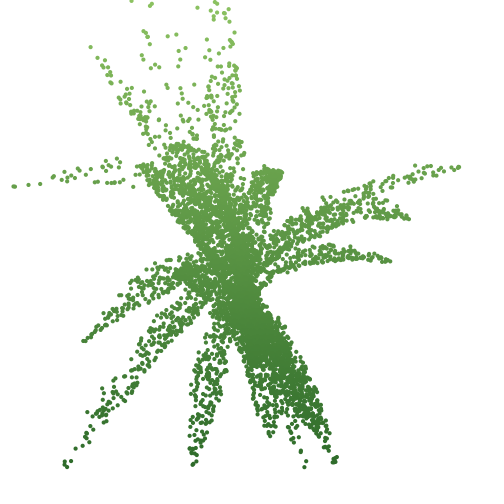
\includegraphics[width=0.8400in, height=0.8400in]{Figures/fig3/sorghum_pc.png}};
\node[anchor=base, inner sep=0, text=cA8456E, rotate=0, font={\fontsize{6.2}{7.4}\selectfont\sffamily\bfseries}] at (5.1633,3.4925) {Point Cloud};
\draw[draw=c9D8CC4, line width=1.00pt, rounded corners=3.60pt, fill=cEAE7F2] (5.8650,2.4775) rectangle (6.7650,3.3775);
\node[anchor=south west, inner sep=0] at (5.8950,2.5075) {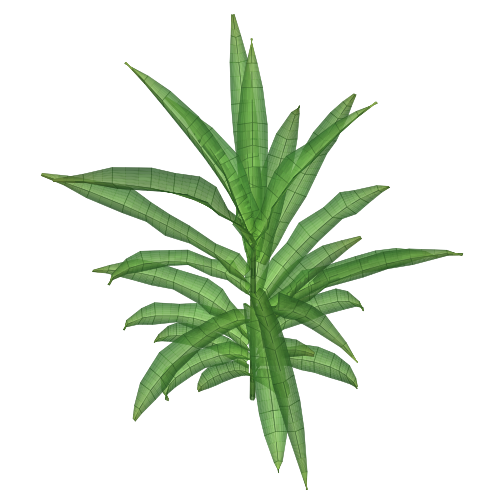
\includegraphics[width=0.8400in, height=0.8400in]{Figures/fig3/sorghum_text.png}};
\node[anchor=base, inner sep=0, text=c5E4A96, rotate=0, font={\fontsize{6.2}{7.4}\selectfont\sffamily\bfseries}] at (6.3150,3.4925) {Procedural Model};
\draw[draw=c809EC2, line width=1.00pt, rounded corners=4.32pt, fill=cE6ECF3] (0.2400,1.3100) rectangle (1.7500,2.3450);
\node[anchor=center, inner sep=0, text=c111111, rotate=90, font={\fontsize{7.0}{8.4}\selectfont\sffamily\bfseries}] at (0.1500,1.8275) {Maize};
\node[anchor=south west, inner sep=0] at (0.3000,1.8450) {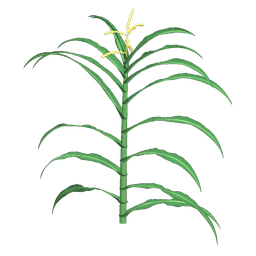
\includegraphics[width=0.4400in, height=0.4400in]{Figures/fig3/maize_gallery_0.png}};
\node[anchor=south west, inner sep=0] at (0.7750,1.8450) {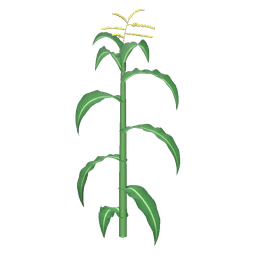
\includegraphics[width=0.4400in, height=0.4400in]{Figures/fig3/maize_gallery_1.png}};
\node[anchor=south west, inner sep=0] at (1.2500,1.8450) {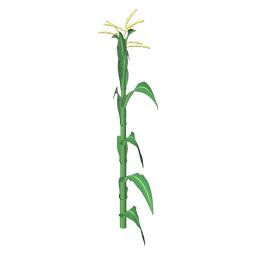
\includegraphics[width=0.4400in, height=0.4400in]{Figures/fig3/maize_gallery_2.png}};
\node[anchor=south west, inner sep=0] at (0.3000,1.3700) {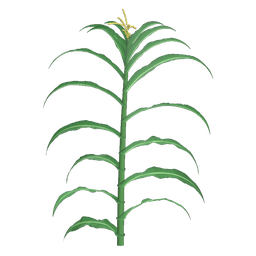
\includegraphics[width=0.4400in, height=0.4400in]{Figures/fig3/maize_gallery_3.png}};
\node[anchor=south west, inner sep=0] at (0.7750,1.3700) {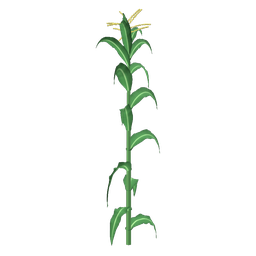
\includegraphics[width=0.4400in, height=0.4400in]{Figures/fig3/maize_gallery_4.png}};
\node[anchor=south west, inner sep=0] at (1.2500,1.3700) {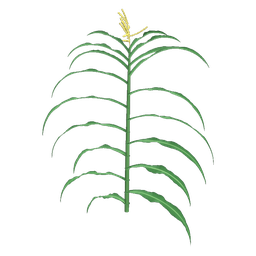
\includegraphics[width=0.4400in, height=0.4400in]{Figures/fig3/maize_gallery_5.png}};
\draw[draw=c333333, line width=1.00pt, rounded corners=2.16pt] (1.2350,1.3550) rectangle (1.7050,1.8250);
\draw[draw=c9A9A9A, line width=0.60pt] (1.7050,1.8250) -- (2.3700,2.3175);
\draw[draw=c9A9A9A, line width=0.60pt] (1.7050,1.3550) -- (2.3700,1.3375);
\draw[draw=c9A9A9A, line width=1.00pt, rounded corners=4.32pt, fill=cF4F4F5] (2.3700,1.3375) rectangle (6.8050,2.3175);
\draw[draw=c809EC2, line width=1.00pt, rounded corners=3.60pt, fill=cE6ECF3] (2.4100,1.3775) rectangle (3.3100,2.2775);
\node[anchor=south west, inner sep=0] at (2.4400,1.4075) {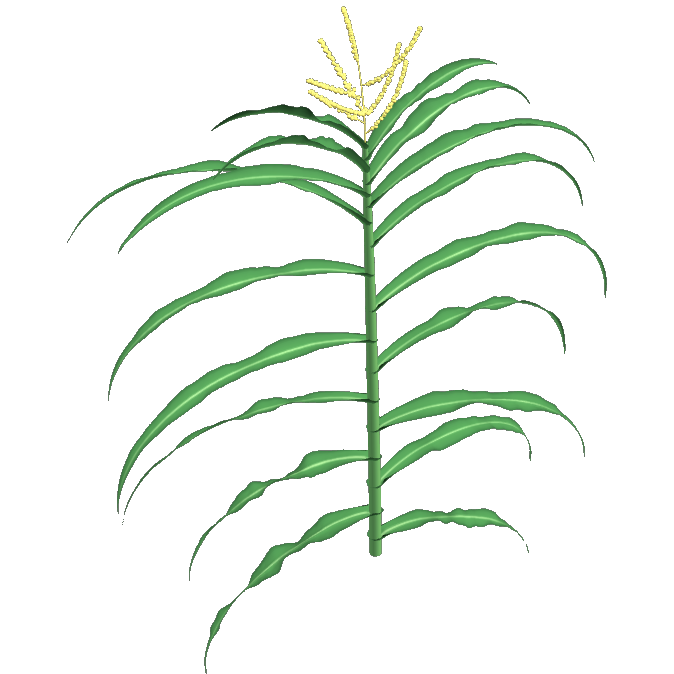
\includegraphics[width=0.8400in, height=0.8400in]{Figures/fig3/maize_rgb.png}};
\draw[draw=cE0B020, line width=1.00pt, rounded corners=3.60pt, fill=cFAF2D4] (3.5617,1.3775) rectangle (4.4617,2.2775);
\node[anchor=south west, inner sep=0] at (3.5917,1.4075) {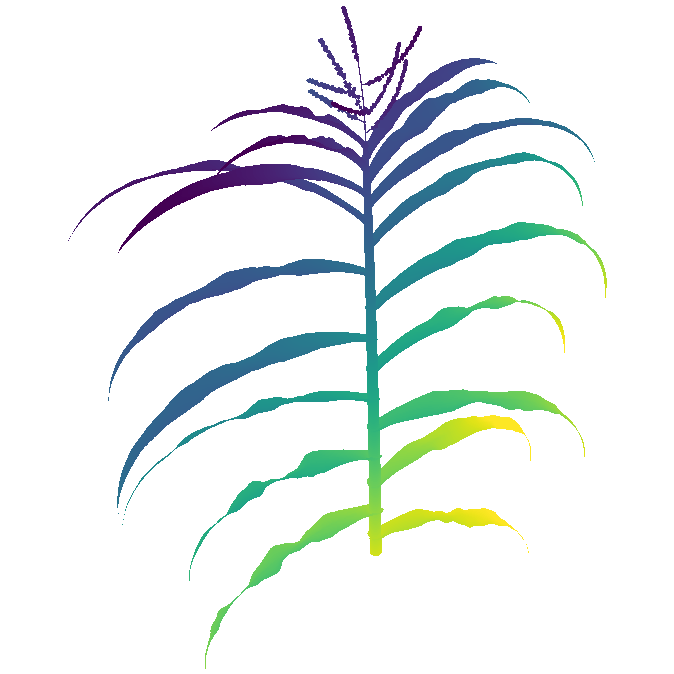
\includegraphics[width=0.8400in, height=0.8400in]{Figures/fig3/maize_depth.png}};
\draw[draw=cD091A7, line width=1.00pt, rounded corners=3.60pt, fill=cF6E9ED] (4.7133,1.3775) rectangle (5.6133,2.2775);
\node[anchor=south west, inner sep=0] at (4.7433,1.4075) {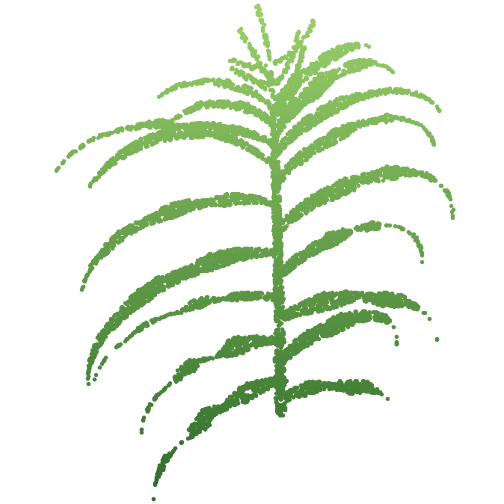
\includegraphics[width=0.8400in, height=0.8400in]{Figures/fig3/maize_pc.png}};
\draw[draw=c9D8CC4, line width=1.00pt, rounded corners=3.60pt, fill=cEAE7F2] (5.8650,1.3775) rectangle (6.7650,2.2775);
\node[anchor=south west, inner sep=0] at (5.8950,1.4075) {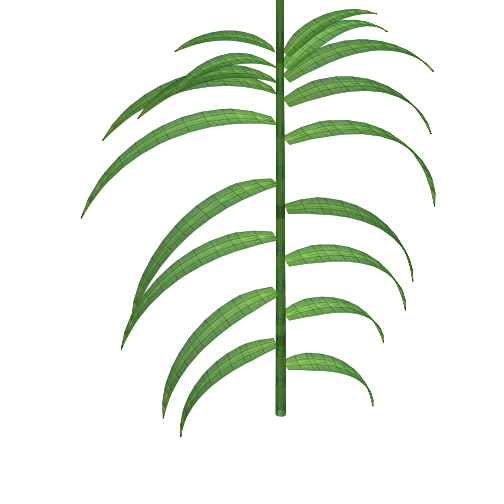
\includegraphics[width=0.8400in, height=0.8400in]{Figures/fig3/maize_text.png}};
\node[anchor=base west, inner sep=0, text=c111111, rotate=0, font={\fontsize{9.0}{10.8}\selectfont\sffamily\bfseries}] at (0.0200,1.1300) {c};
\node[anchor=base west, inner sep=0, text=c111111, rotate=0, font={\fontsize{6.2}{7.4}\selectfont\sffamily}] at (0.1800,1.1300) {Ten cameras per plant (five shown), by elevation};
\draw[draw=c809EC2, line width=1.00pt, rounded corners=2.88pt, fill=cE6ECF3] (0.2600,0.5600) rectangle (2.1800,0.9800);
\node[anchor=center, inner sep=0, text=c111111, rotate=90, font={\fontsize{5.8}{7.0}\selectfont\sffamily\bfseries}] at (0.1500,0.7700) {Sorghum};
\node[anchor=south west, inner sep=0] at (0.3000,0.6000) {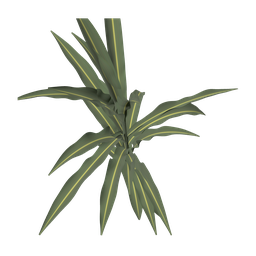
\includegraphics[width=0.3400in, height=0.3400in]{Figures/fig3/sorghum_camera_0.png}};
\node[anchor=south, inner sep=0, text=c444444, rotate=0, font={\fontsize{5.4}{6.5}\selectfont\sffamily}] at (0.4700,0.9900) {+64$^{\circ}$};
\node[anchor=south west, inner sep=0] at (0.6750,0.6000) {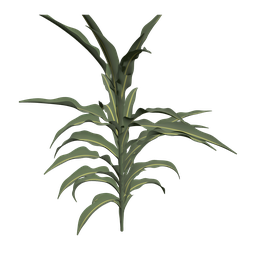
\includegraphics[width=0.3400in, height=0.3400in]{Figures/fig3/sorghum_camera_1.png}};
\node[anchor=south, inner sep=0, text=c444444, rotate=0, font={\fontsize{5.4}{6.5}\selectfont\sffamily}] at (0.8450,0.9900) {+30$^{\circ}$};
\node[anchor=south west, inner sep=0] at (1.0500,0.6000) {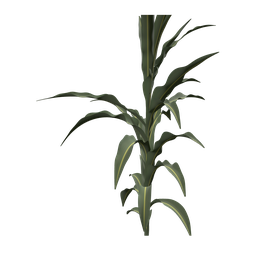
\includegraphics[width=0.3400in, height=0.3400in]{Figures/fig3/sorghum_camera_2.png}};
\node[anchor=south, inner sep=0, text=c444444, rotate=0, font={\fontsize{5.4}{6.5}\selectfont\sffamily}] at (1.2200,0.9900) {+6$^{\circ}$};
\node[anchor=south west, inner sep=0] at (1.4250,0.6000) {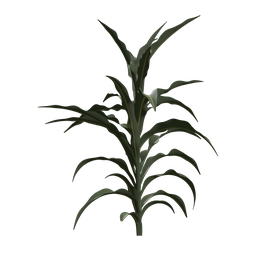
\includegraphics[width=0.3400in, height=0.3400in]{Figures/fig3/sorghum_camera_3.png}};
\node[anchor=south, inner sep=0, text=c444444, rotate=0, font={\fontsize{5.4}{6.5}\selectfont\sffamily}] at (1.5950,0.9900) {$-$17$^{\circ}$};
\node[anchor=south west, inner sep=0] at (1.8000,0.6000) {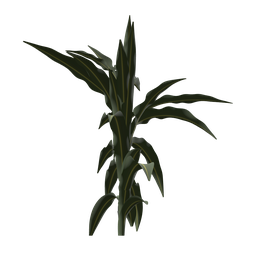
\includegraphics[width=0.3400in, height=0.3400in]{Figures/fig3/sorghum_camera_4.png}};
\node[anchor=south, inner sep=0, text=c444444, rotate=0, font={\fontsize{5.4}{6.5}\selectfont\sffamily}] at (1.9700,0.9900) {$-$44$^{\circ}$};
\draw[draw=c809EC2, line width=1.00pt, rounded corners=2.88pt, fill=cE6ECF3] (0.2600,0.0300) rectangle (2.1800,0.4500);
\node[anchor=center, inner sep=0, text=c111111, rotate=90, font={\fontsize{5.8}{7.0}\selectfont\sffamily\bfseries}] at (0.1500,0.2400) {Maize};
\node[anchor=south west, inner sep=0] at (0.3000,0.0700) {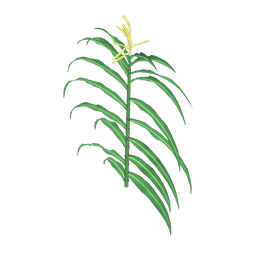
\includegraphics[width=0.3400in, height=0.3400in]{Figures/fig3/maize_camera_0.png}};
\node[anchor=south, inner sep=0, text=c444444, rotate=0, font={\fontsize{5.4}{6.5}\selectfont\sffamily}] at (0.4700,0.4600) {+39$^{\circ}$};
\node[anchor=south west, inner sep=0] at (0.6750,0.0700) {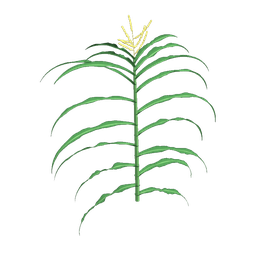
\includegraphics[width=0.3400in, height=0.3400in]{Figures/fig3/maize_camera_1.png}};
\node[anchor=south, inner sep=0, text=c444444, rotate=0, font={\fontsize{5.4}{6.5}\selectfont\sffamily}] at (0.8450,0.4600) {+30$^{\circ}$};
\node[anchor=south west, inner sep=0] at (1.0500,0.0700) {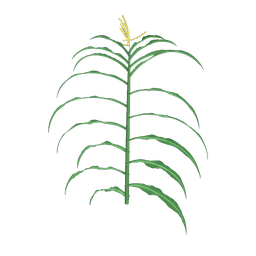
\includegraphics[width=0.3400in, height=0.3400in]{Figures/fig3/maize_camera_2.png}};
\node[anchor=south, inner sep=0, text=c444444, rotate=0, font={\fontsize{5.4}{6.5}\selectfont\sffamily}] at (1.2200,0.4600) {+10$^{\circ}$};
\node[anchor=south west, inner sep=0] at (1.4250,0.0700) {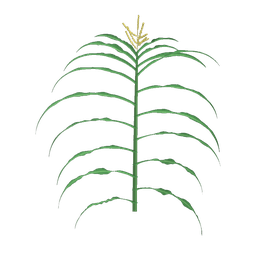
\includegraphics[width=0.3400in, height=0.3400in]{Figures/fig3/maize_camera_3.png}};
\node[anchor=south, inner sep=0, text=c444444, rotate=0, font={\fontsize{5.4}{6.5}\selectfont\sffamily}] at (1.5950,0.4600) {$-$13$^{\circ}$};
\node[anchor=south west, inner sep=0] at (1.8000,0.0700) {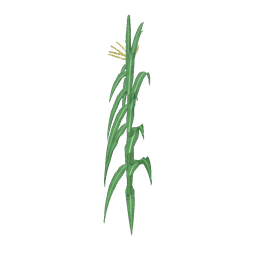
\includegraphics[width=0.3400in, height=0.3400in]{Figures/fig3/maize_camera_4.png}};
\node[anchor=south, inner sep=0, text=c444444, rotate=0, font={\fontsize{5.4}{6.5}\selectfont\sffamily}] at (1.9700,0.4600) {$-$36$^{\circ}$};
\node[anchor=base west, inner sep=0, text=c111111, rotate=0, font={\fontsize{9.0}{10.8}\selectfont\sffamily\bfseries}] at (2.8400,1.1300) {d};
\node[anchor=base west, inner sep=0, text=c111111, rotate=0, font={\fontsize{6.2}{7.4}\selectfont\sffamily}] at (3.0000,1.1300) {Crop rows: the target plant between neighbors};
\node[anchor=base west, inner sep=0, text=c555555, rotate=0, font={\fontsize{5.4}{6.5}\selectfont\sffamily}] at (3.0000,1.0250) {\textcolor{cLegRed}{\textbf{Red}}: Neighbor pixels  \textcolor{cLegOrange}{\textbf{Orange}}: Target pixels occluded by neighbors (\% hidden)  \textcolor{cLegGreen}{\textbf{Green}}: Target points};
\node[anchor=base, inner sep=0, text=c111111, rotate=0, font={\fontsize{6.2}{7.4}\selectfont\sffamily\bfseries}] at (3.7600,0.9350) {Sorghum};
\draw[draw=c809EC2, line width=1.00pt, rounded corners=3.60pt, fill=cE6ECF3] (2.9900,0.1300) rectangle (3.7500,0.8900);
\node[anchor=south west, inner sep=0] at (3.0200,0.1600) {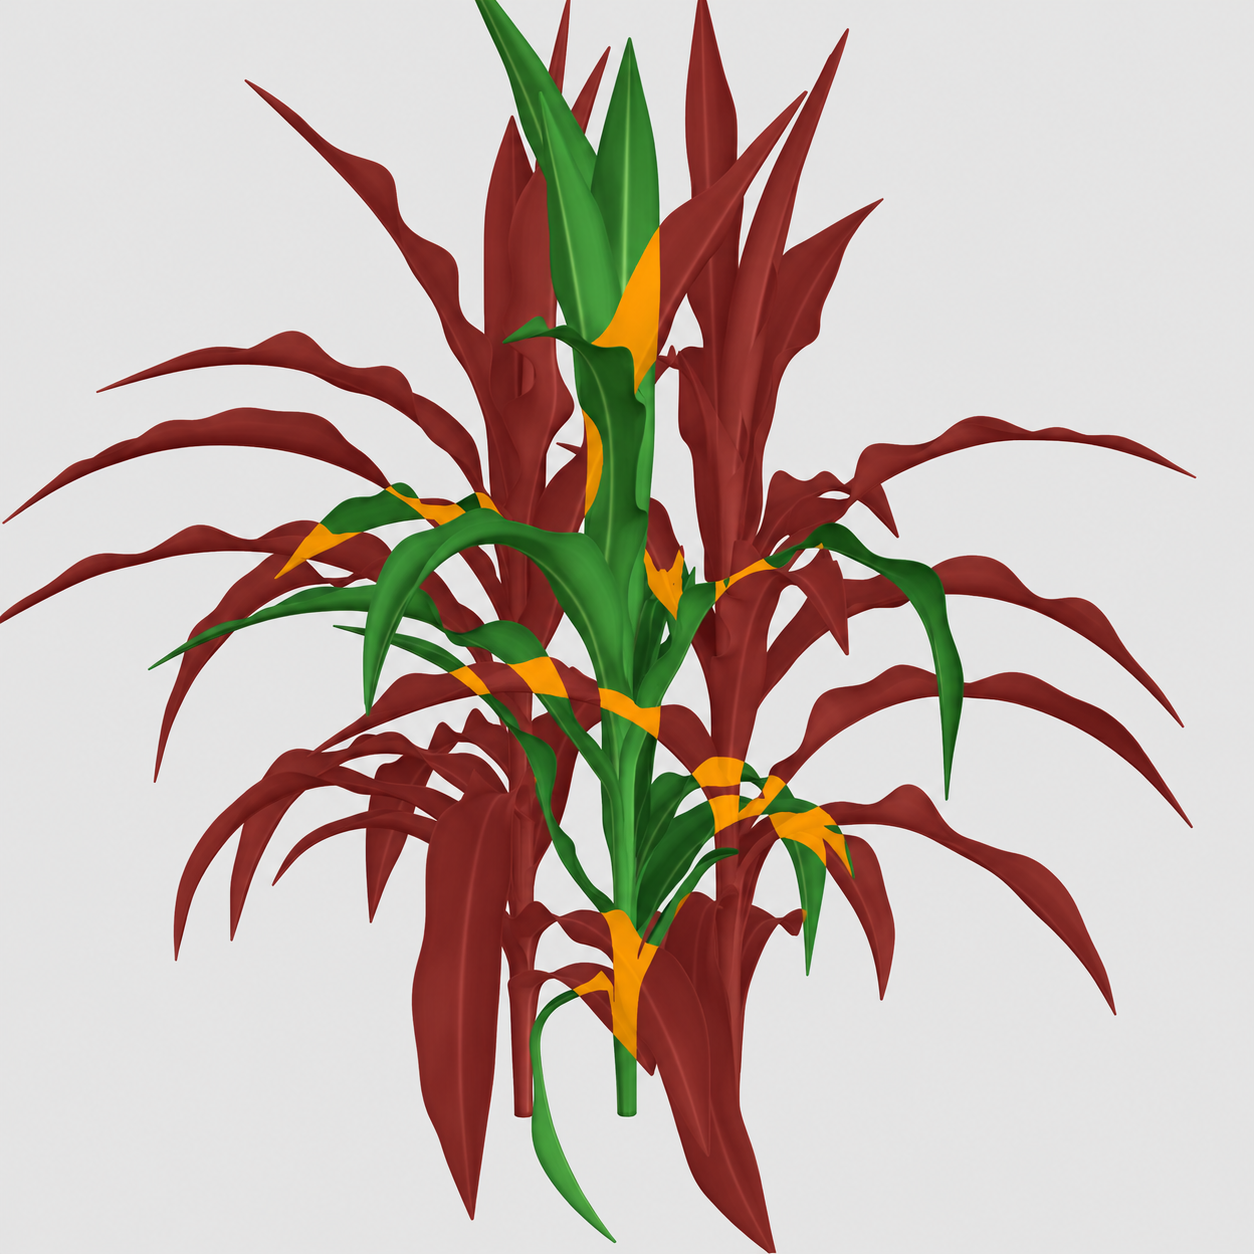
\includegraphics[width=0.7000in, height=0.7000in]{Figures/fig3/sorghum_row_image.png}};
\node[anchor=north, inner sep=0, text=c111111, rotate=0, font={\fontsize{5.6}{6.7}\selectfont\sffamily}] at (3.3700,0.1000) {16 \% hidden};
\draw[draw=cD091A7, line width=1.00pt, rounded corners=3.60pt, fill=cF6E9ED] (3.7700,0.1300) rectangle (4.5300,0.8900);
\node[anchor=south west, inner sep=0] at (3.8000,0.1600) {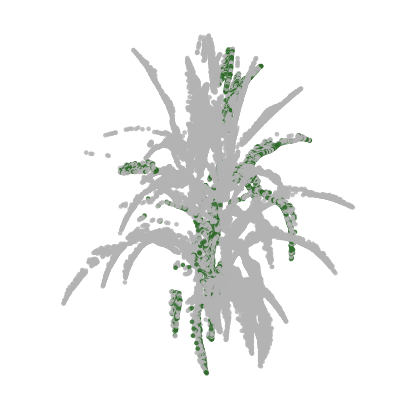
\includegraphics[width=0.7000in, height=0.7000in]{Figures/fig3/sorghum_row_cloud.png}};
\node[anchor=north, inner sep=0, text=c111111, rotate=0, font={\fontsize{5.6}{6.7}\selectfont\sffamily}] at (4.1500,0.1000) {89 \% neighbors};
\node[anchor=base, inner sep=0, text=c111111, rotate=0, font={\fontsize{6.2}{7.4}\selectfont\sffamily\bfseries}] at (5.5400,0.9350) {Maize};
\draw[draw=c809EC2, line width=1.00pt, rounded corners=3.60pt, fill=cE6ECF3] (4.7700,0.1300) rectangle (5.5300,0.8900);
\node[anchor=south west, inner sep=0] at (4.8000,0.1600) {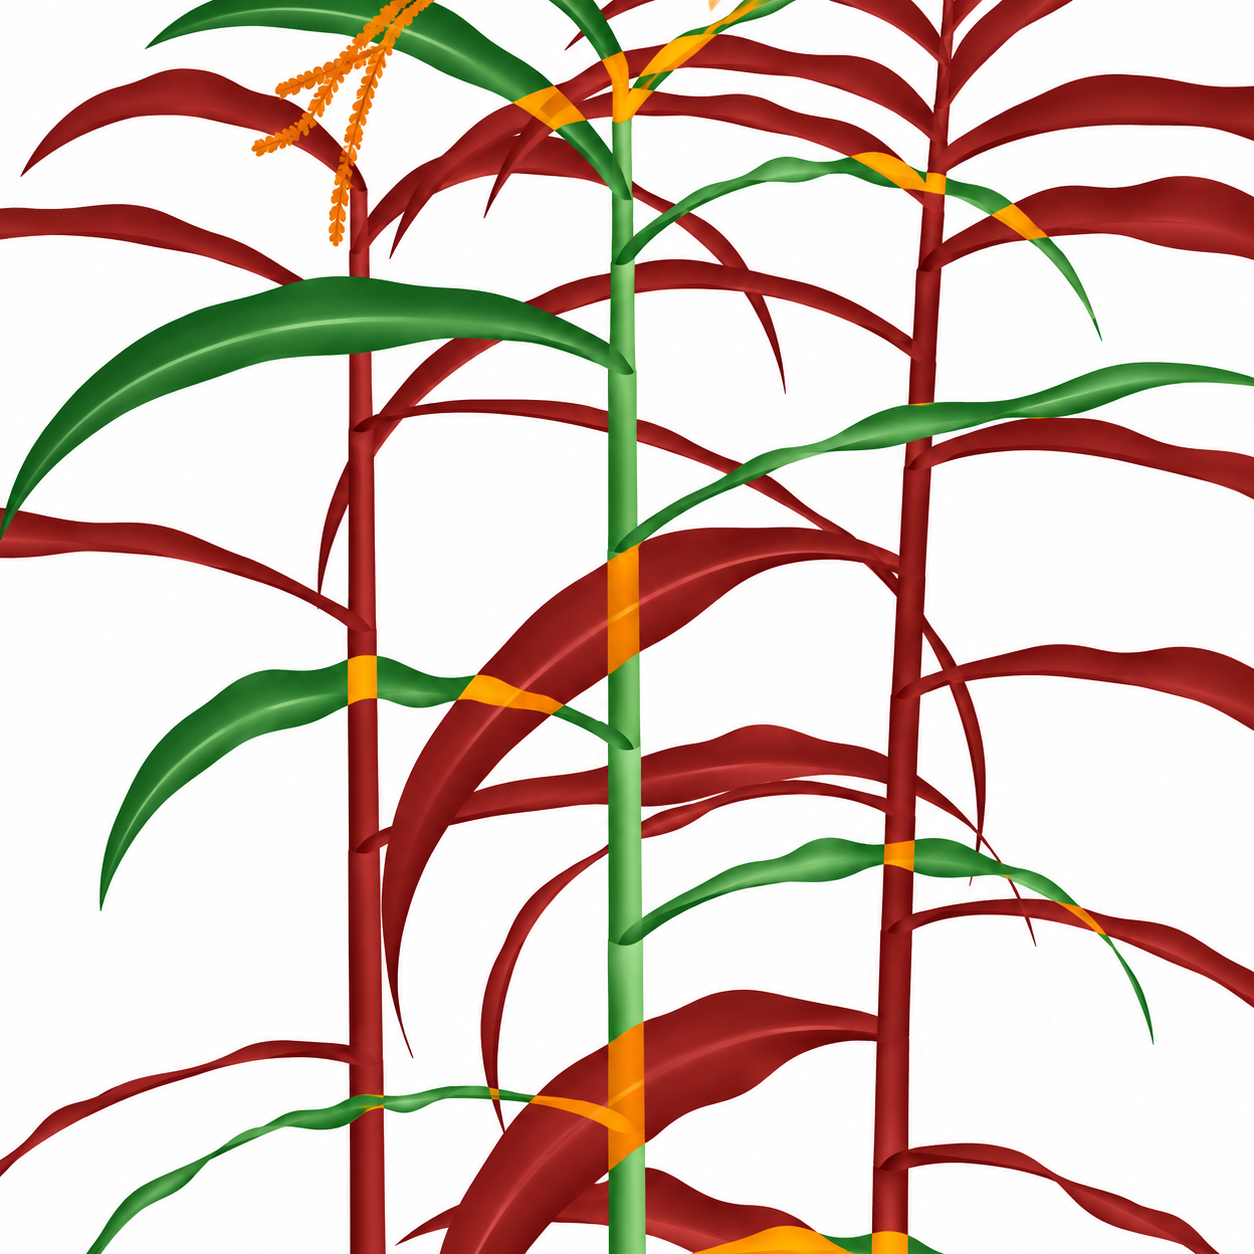
\includegraphics[width=0.7000in, height=0.7000in]{Figures/fig3/maize_row_image.png}};
\node[anchor=north, inner sep=0, text=c111111, rotate=0, font={\fontsize{5.6}{6.7}\selectfont\sffamily}] at (5.1500,0.1000) {15 \% hidden};
\draw[draw=cD091A7, line width=1.00pt, rounded corners=3.60pt, fill=cF6E9ED] (5.5500,0.1300) rectangle (6.3100,0.8900);
\node[anchor=south west, inner sep=0] at (5.5800,0.1600) {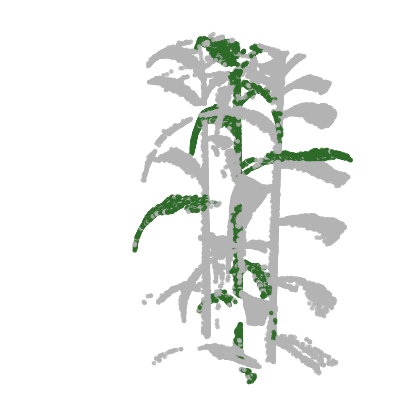
\includegraphics[width=0.7000in, height=0.7000in]{Figures/fig3/maize_row_cloud.png}};
\node[anchor=north, inner sep=0, text=c111111, rotate=0, font={\fontsize{5.6}{6.7}\selectfont\sffamily}] at (5.9300,0.1000) {75 \% neighbors};
\end{tikzpicture}
}
    \vspace{-15pt}

  \caption{\textbf{Overview of the \dataset{} benchmark.} \textbf{(a)} Six example validation plants per species from a side view, illustrating the morphological diversity across the 15{,}000 generated plants per crop. \textbf{(b)} The four aligned data streams for one camera view of the highlighted plant (RGB image, metric depth map, camera-frame 3D point cloud, and procedural model drawn as a stem-and-leaf schematic). \textbf{(c)} Five of ten camera viewpoints per plant (see \secref{sec:isolated-rendering} for sampling details). \textbf{(d)} Simulated crop rows with heavy inter-plant occlusion. In RGB, neighbors are red and hidden target pixels are orange; in the point cloud, target points are green and occluding neighbors are grey.}
  \label{fig:dataset}
\end{figure*}
\begin{table}[t]
  \caption{\textbf{Comparison with existing 3D plant and shape completion benchmarks.} ``Exact proc.\ GT'' denotes exact generative parameters per plant, and (\cmark) indicates parameters fitted post hoc via optimization. $^{\dagger}$\dataset{} includes an evaluation split of rendered rows built from real plant scans, alongside the synthetic training data.}
  \label{tab:datacompare}
  \centering\scriptsize
  \setlength{\tabcolsep}{1.3pt}
  \renewcommand{\arraystretch}{1.8}
  \resizebox{\columnwidth}{!}{%
  \begin{tabular}{lcccccc}
  \toprule
  Dataset & Real scans & Slender & Row occl. & RGB+D+PC & Exact proc.\ GT & Scale \\
  \midrule
  PCN / ShapeNet-55~\citep{yuan2018pcn,yu2021pointr} & \xmark & \xmark & \xmark & \xmark & \xmark & 55{,}000 \\
  Pheno4D~\citep{schunck2021pheno4d} & \cmark & \cmark & \xmark & \xmark & \xmark & 84 \\
  Crops3D~\citep{crops3d2024} & \cmark & \cmark & \xmark & \xmark & \xmark & 2{,}500 \\
  MaizeField3D~\citep{maizefield3d2025} & \cmark & \cmark & \xmark & \xmark & (\cmark) & 1{,}000 \\
  \textbf{\dataset{} (ours)} & \textbf{\cmark}$^{\dagger}$ & \textbf{\cmark} & \textbf{\cmark} & \textbf{\cmark} & \textbf{\cmark} & \textbf{30{,}000} \\
  \bottomrule
  \end{tabular}}
\end{table}

\noindent\textbf{Isolated plants.}
We build species-specific procedural generators, following a long line of bespoke plant generators~\citep{prusin1990abop,fournier1998maize,boudon2012lpy,cieslak2024agdata,floraforge2026,hadadi2025procmaize,vazquez_phenoframe_2026,ostermann_sorghum_2024}. Using these generators, we synthesize 15{,}000 plants each for maize and sorghum. Maize plants span 0.62 to 1.44\,m in height with 3 to 22 leaves, and height and leaf count are only weakly correlated ($r = 0.20$). Sorghum plants have stem lengths of 0.19 to 1.74\,m and 4 to 35 leaves, and the leaf count is tightly coupled to the stem length ($R^2 = 0.988$). The two species thus cover both weakly and strongly coupled morphologies. We render ten views per plant with RGB and metric depth at $1{,}024 \times 1{,}024$ resolution along with camera calibration, and we store an 8{,}192-point cloud per view. Sorghum is captured from a fixed ten-camera rig with a complete plant cloud per view, whereas maize is captured from random directions with a partial cloud back-projected from the depth map. We split the plants 70\% / 15\% / 15\% into train, validation, and test sets, and we enrich the validation and test splits toward extreme morphologies.

\noindent\textbf{Crop rows.}
To simulate field rows, we place each target plant between two neighbors spaced 0.15\,m apart, at ten row orientations ($0^\circ$ to $90^\circ$ yaw),  which is consistent with modern agronomic planting densities. Placing plant meshes side by side makes their leaves pass through one another. We therefore develop an articulated contact solver that models leaf blades as chains of 8\,cm jointed segments and resolves all triangle-triangle collisions. The neighbors yield first, and the target plant retains its grown shape wherever possible. A simulated ground-rover camera captures the crowded row (RGB, depth, and a 24{,}576-point scene cloud). The ground truth is the contact-bent target plant alone (an 8{,}192-point cloud and its procedural parameters). In these rows, neighbors account for 59 to 68\% of all plant pixels in maize and occlude 23\% of the target plant's pixels in sorghum.

\noindent\textbf{Real plants.}
To evaluate on real morphology, we also assemble rows from the procedural models of 520 real maize plants released with MaizeField3D~\citep{maizefield3d2025} and from 30 laser-scanned real sorghum plants (\secref{sec:exp-real}). The generation, rendering, and contact-solver details can be found in the Appendix.
% APPENDIX REF (removed for submission, restore later): \appendixref{app:data} (for: can be found in the Appendix)

\subsection{All-Modality Masked Pretraining}
\label{sec:method-pretrain}

\noindent\textbf{Tokenization.}
We extend EmbodiedMAE~\citep{dong2025embodiedmae} with a fourth stream for the procedural parameters. RGB and depth images are split into 196 patches each, and point clouds into 196 neighborhoods of 32 points that are encoded with a lightweight PointNet~\citep{pang2022pointmae,qi2017pointnet}. We structure the parameter vector $\theta$ into $1 + K$ continuous numerical tokens, i.e., one global plant token followed by $K$ ordered leaf slots ($K = 28$ for maize, $K = 24$ for sorghum), embedded using xVal-style continuous value scaling~\citep{golkar2023xval}. The visible tokens and a global \texttt{[CLS]} token are processed by a 12-block ViT encoder (width 768) and reconstructed by an 8-block decoder (width 512) with one output head per stream (see the Appendix).
% APPENDIX REF (removed for submission, restore later): (\appendixref{app:impl}) (for: please see Appendix)
% \appendixref{app:impl}).

\noindent\textbf{Masking.}
To train a single network that can handle any subset of sensor inputs, we mask a fraction $\rho = 0.80$ of all tokens at each step ($122$ of $L = 613$ tokens remain visible in sorghum, and $123$ of $617$ in maize). The visible tokens are allocated across the four streams using a symmetric Dirichlet draw at every iteration. Note that the parameter stream takes part in this masking ($\sim 58\%$ of its tokens are visible on average). The network thus also learns to use known parameters as an input. At inference, the parameters are the output, and no parameter token is given. %unless stated otherwise.

\noindent\textbf{Reconstruction objective.}
We train the network with a weighted sum of modality-specific reconstruction losses:
\begin{equation}
  \mathcal{L}_{\mathrm{rec}} = \ell_{\mathrm{rgb}} + \ell_{\mathrm{d}} + \ell_{\mathrm{pc}} + 5\ell_\theta,
  \label{eq:reconstruction-loss}
\end{equation}
where $\ell_{\mathrm{rgb}}$ is the MSE on patch-normalized RGB pixels~\citep{he2022mae}, $\ell_{\mathrm{d}}$ is the MSE on min-max normalized depth, and $\ell_\theta$ is the Smooth-$L_1$ loss on masked parameter tokens. The point-cloud term requires care for thin geometry. With the standard Chamfer distance, a decoder can reduce the error by clustering points onto thick stems while omitting thin leaf blades~\citep{wu2021dcd,song2026structural}. We therefore use a sigmoid-weighted quality-aware loss~\citep{meshram2026qal} (QAL, see the Appendix) for $\ell_{\mathrm{pc}}$. It weights the nearest-neighbor distances with a sigmoid of sharpness $100$ around a tolerance of $\tau = 0.01$ (unit-sphere coordinates), which focuses the gradients on poorly reconstructed regions. We further add a debiased Sinkhorn divergence~\citep{feydy2019sinkhorn} over 1{,}024-point subsets ($\varepsilon = 0.0004$) to encourage global coverage of thin foliage:
% APPENDIX REF (removed for submission, restore later): (QAL, Eq.~\eqref{eq:qal} in \appendixref{sec:abl_loss}) (for: QAL, see Appendix)
\begin{equation}
  \ell_{\mathrm{pc}}^{\star} = \ell_{\mathrm{pc}} + 0.5\,S_{\varepsilon}\!\left(\hat P_{1024}, P_{1024}\right).
  \label{eq:point-loss-sinkhorn}
\end{equation}
The combination gives a higher $F_1$ than either term alone (see the Appendix). We train with AdamW and cosine learning-rate decay for 1{,}000 epochs over all ten views (global batch size 256, peak learning rate $6 \times 10^{-4}$).
% APPENDIX REF (removed for submission, restore later): (\appendixref{sec:abl_loss}) (for: please see Appendix)

\subsection{Distillation into Single-Sensor Students}
\label{sec:distill}\label{sec:method-distill}

The first specialization is designed for single-sensor inference. At deployment, a single-sensor model sees one modality while all tokens of the remaining streams are absent. This configuration is rare under random Dirichlet masking, and we therefore distill a frozen four-stream teacher into single-sensor students. The teacher is the pretrained model with privileged access to the procedural parameters. %(all parameter tokens visible for sorghum, and 50\% of each stream visible for maize, where full visibility degrades cloud reconstruction).
It produces a global latent vector $c^T \in \R^{768}$ and normalized decoder features $F^T \in \R^{L \times 512}$. Each student is initialized from the teacher's weights and trained for 100 epochs (AdamW, learning rate $10^{-4}$, global batch size 128). On 80\% of the training steps, the student receives a single source stream $s \in \{\mathrm{rgb}, \mathrm{d}, \mathrm{pc}, \theta\}$ with all other streams masked. On the remaining 20\%, it follows the four-stream masked pretraining. The student minimizes
\begin{equation}
  \mathcal{L}_{\mathrm{student}} = \mathcal{L}_{\mathrm{rec}} + \frac{\lambda_F}{|\mathcal{J}_{\neg s}|} \sum_{j \in \mathcal{J}_{\neg s}} \|F^S_j - F^T_j\|_2^2 + \lambda_c \|c^S - c^T\|_2^2,
  \label{eq:distillation-loss}
\end{equation}
where $\mathcal{J}_{\neg s}$ indexes the decoder positions of the unobserved streams, $\lambda_F = 1.0$, and $\lambda_c = 0.5$. %Our experiments use a single generalist student that is trained across all source streams.


\subsection{Row-Occlusion Fine-Tuning}
\label{sec:method-rows}

The second specialization is designed for plants in crop rows. The pretraining data, however, contain only isolated plants. We therefore fine-tune the pretrained (Stage~1) model on the simulated rows of \secref{sec:method-data}. The input is the crowded row (RGB, depth, and the 24{,}576-point scene cloud), and the reconstruction losses are computed on the contact-bent target plant alone. The model does not receive a bounding box or mask, and it has to identify the target plant from the row itself. We fine-tune for 100 epochs using AdamW (learning rate $10^{-4}$, global batch size 32, 5 warmup epochs) at the pretraining mask ratio of 0.8.


%%%%%%%%%%%%%%%%%%%%%%%%%%%%%%%%%%%%%%%%%%%%%%%%%%%%%%%%%%%%%%%%%%%%%%%%%%%
% 4. EXPERIMENTS
%%%%%%%%%%%%%%%%%%%%%%%%%%%%%%%%%%%%%%%%%%%%%%%%%%%%%%%%%%%%%%%%%%%%%%%%%%%
\section{Experiments}
\label{sec:results}\label{sec:experiments}

\begin{figure*}[t]
  \centering
  \resizebox{\linewidth}{!}{% Generated by figures/_scene.py (Scene.render_tikz) for 'Fig 5 crop-row examples (procedural)'; do not edit by hand, re-run the figure script.
% 6.875 x 3.3400000000000003 in at 100 %; needs \usetikzlibrary{arrows.meta}; images in Figures/fig5/.
{%
\definecolor{c1A1A1A}{HTML}{1A1A1A}%
\definecolor{c1D221C}{HTML}{1D221C}%
\definecolor{c5E4A96}{HTML}{5E4A96}%
\definecolor{c809EC2}{HTML}{809EC2}%
\definecolor{c9A9A9A}{HTML}{9A9A9A}%
\definecolor{c9D8CC4}{HTML}{9D8CC4}%
\definecolor{cE6ECF3}{HTML}{E6ECF3}%
\definecolor{cEAE7F2}{HTML}{EAE7F2}%
\definecolor{cF4F4F5}{HTML}{F4F4F5}%
\begin{tikzpicture}[x=1in, y=1in]%
\useasboundingbox (0,0) rectangle (6.8750,3.3400);
\draw[draw=c809EC2, line width=1.000pt, fill=cE6ECF3, dash pattern=on 3.00pt off 2.00pt, rounded corners=0.0500in] (0.6200,1.9600) rectangle (1.5200,2.8600);
\draw[draw=c9A9A9A, line width=1.000pt, fill=cF4F4F5, rounded corners=0.0500in] (1.5700,1.9600) rectangle (2.4700,2.8600);
\draw[draw=c9D8CC4, line width=1.000pt, fill=cEAE7F2, rounded corners=0.0500in] (2.5200,1.9600) rectangle (3.4200,2.8600);
\draw[draw=c809EC2, line width=1.000pt, fill=cE6ECF3, dash pattern=on 3.00pt off 2.00pt, rounded corners=0.0500in] (0.6200,0.9900) rectangle (1.5200,1.8900);
\draw[draw=c9A9A9A, line width=1.000pt, fill=cF4F4F5, rounded corners=0.0500in] (1.5700,0.9900) rectangle (2.4700,1.8900);
\draw[draw=c9D8CC4, line width=1.000pt, fill=cEAE7F2, rounded corners=0.0500in] (2.5200,0.9900) rectangle (3.4200,1.8900);
\draw[draw=c809EC2, line width=1.000pt, fill=cE6ECF3, dash pattern=on 3.00pt off 2.00pt, rounded corners=0.0500in] (0.6200,0.0200) rectangle (1.5200,0.9200);
\draw[draw=c9A9A9A, line width=1.000pt, fill=cF4F4F5, rounded corners=0.0500in] (1.5700,0.0200) rectangle (2.4700,0.9200);
\draw[draw=c9D8CC4, line width=1.000pt, fill=cEAE7F2, rounded corners=0.0500in] (2.5200,0.0200) rectangle (3.4200,0.9200);
\draw[draw=c809EC2, line width=1.000pt, fill=cE6ECF3, dash pattern=on 3.00pt off 2.00pt, rounded corners=0.0500in] (3.9950,1.9600) rectangle (4.8950,2.8600);
\draw[draw=c9A9A9A, line width=1.000pt, fill=cF4F4F5, rounded corners=0.0500in] (4.9450,1.9600) rectangle (5.8450,2.8600);
\draw[draw=c9D8CC4, line width=1.000pt, fill=cEAE7F2, rounded corners=0.0500in] (5.8950,1.9600) rectangle (6.7950,2.8600);
\draw[draw=c809EC2, line width=1.000pt, fill=cE6ECF3, dash pattern=on 3.00pt off 2.00pt, rounded corners=0.0500in] (3.9950,0.9900) rectangle (4.8950,1.8900);
\draw[draw=c9A9A9A, line width=1.000pt, fill=cF4F4F5, rounded corners=0.0500in] (4.9450,0.9900) rectangle (5.8450,1.8900);
\draw[draw=c9D8CC4, line width=1.000pt, fill=cEAE7F2, rounded corners=0.0500in] (5.8950,0.9900) rectangle (6.7950,1.8900);
\draw[draw=c809EC2, line width=1.000pt, fill=cE6ECF3, dash pattern=on 3.00pt off 2.00pt, rounded corners=0.0500in] (3.9950,0.0200) rectangle (4.8950,0.9200);
\draw[draw=c9A9A9A, line width=1.000pt, fill=cF4F4F5, rounded corners=0.0500in] (4.9450,0.0200) rectangle (5.8450,0.9200);
\draw[draw=c9D8CC4, line width=1.000pt, fill=cEAE7F2, rounded corners=0.0500in] (5.8950,0.0200) rectangle (6.7950,0.9200);
\node[anchor=south west, inner sep=0] at (0.6500,1.9900) {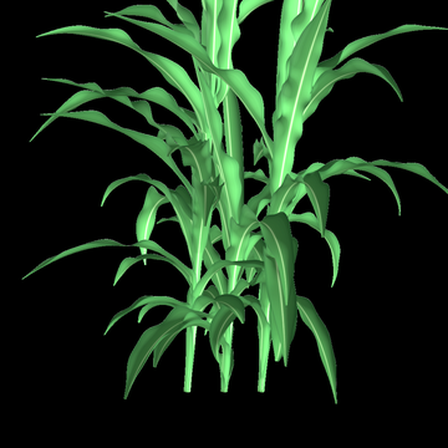
\includegraphics[width=0.8400in, height=0.8400in]{Figures/fig5/sorghum_Sorghum_10756_90_Row_image.png}};
\node[anchor=south west, inner sep=0] at (1.6000,1.9900) {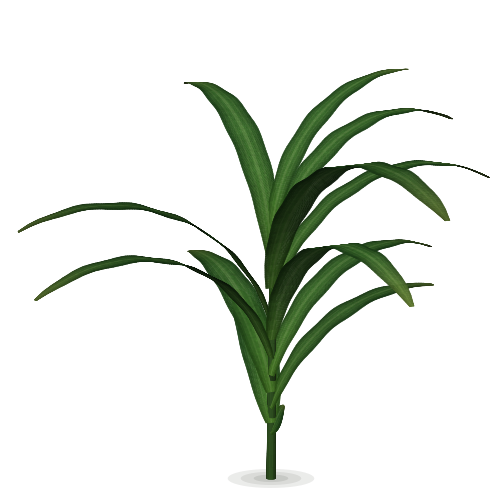
\includegraphics[width=0.8400in, height=0.8400in]{Figures/fig5/sorghum_Sorghum_10756_90_Ground_truth.png}};
\node[anchor=south west, inner sep=0] at (2.5500,1.9900) {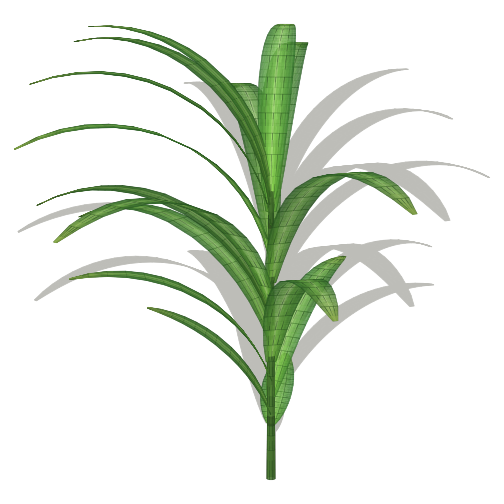
\includegraphics[width=0.8400in, height=0.8400in]{Figures/fig5/sorghum_Sorghum_10756_90_Row_trained.png}};
\node[anchor=south west, inner sep=0] at (0.6500,1.0200) {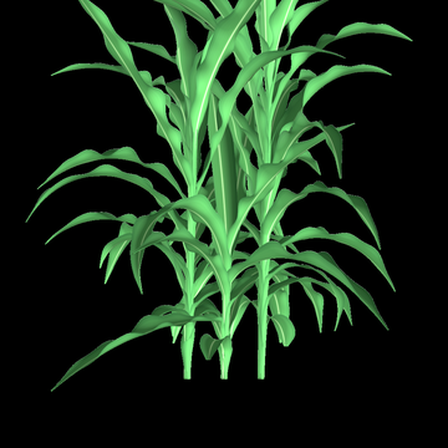
\includegraphics[width=0.8400in, height=0.8400in]{Figures/fig5/sorghum_Sorghum_14816_0_Row_image.png}};
\node[anchor=south west, inner sep=0] at (1.6000,1.0200) {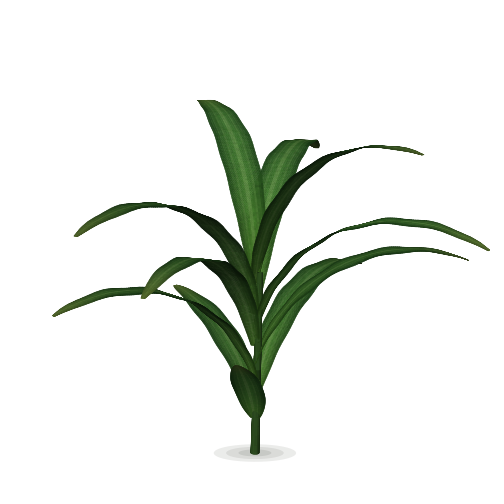
\includegraphics[width=0.8400in, height=0.8400in]{Figures/fig5/sorghum_Sorghum_14816_0_Ground_truth.png}};
\node[anchor=south west, inner sep=0] at (2.5500,1.0200) {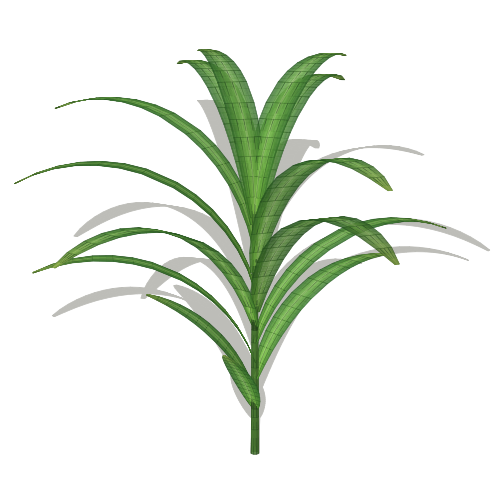
\includegraphics[width=0.8400in, height=0.8400in]{Figures/fig5/sorghum_Sorghum_14816_0_Row_trained.png}};
\node[anchor=south west, inner sep=0] at (0.6500,0.0500) {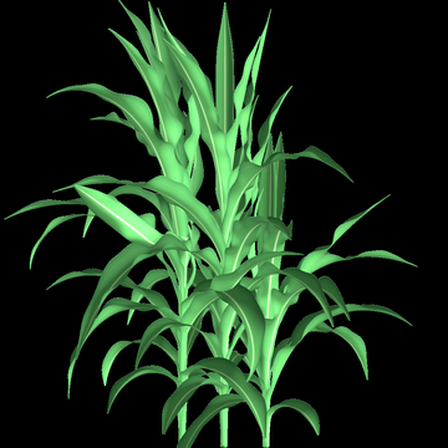
\includegraphics[width=0.8400in, height=0.8400in]{Figures/fig5/sorghum_Sorghum_4815_0_Row_image.png}};
\node[anchor=south west, inner sep=0] at (1.6000,0.0500) {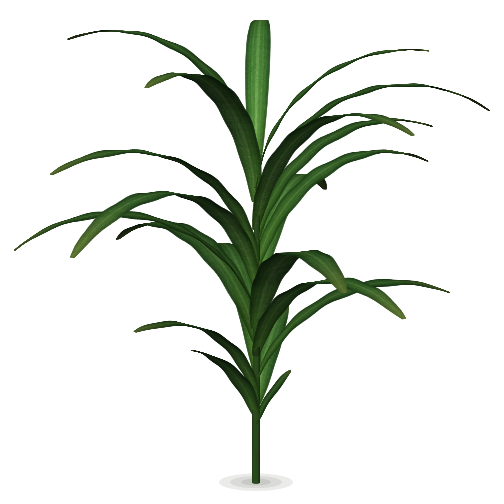
\includegraphics[width=0.8400in, height=0.8400in]{Figures/fig5/sorghum_Sorghum_4815_0_Ground_truth.png}};
\node[anchor=south west, inner sep=0] at (2.5500,0.0500) {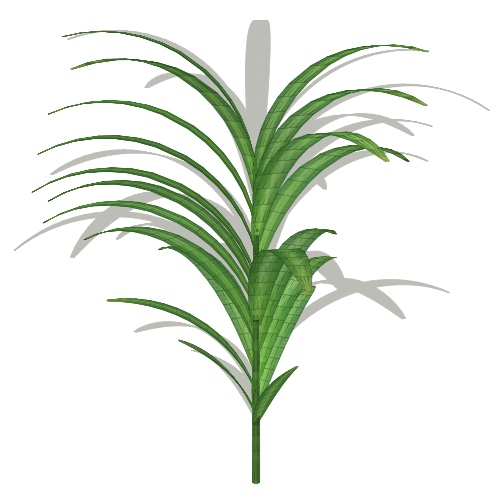
\includegraphics[width=0.8400in, height=0.8400in]{Figures/fig5/sorghum_Sorghum_4815_0_Row_trained.png}};
\node[anchor=south west, inner sep=0] at (4.0250,1.9900) {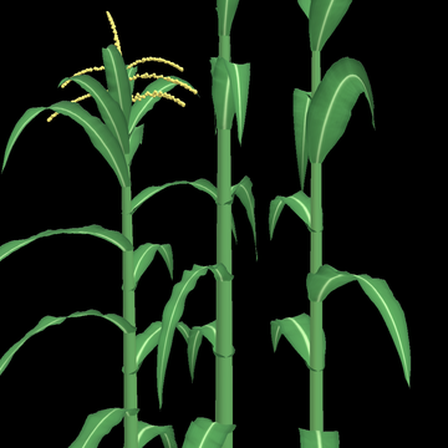
\includegraphics[width=0.8400in, height=0.8400in]{Figures/fig5/maize_plant_0320_90_Row_image.png}};
\node[anchor=south west, inner sep=0] at (4.9750,1.9900) {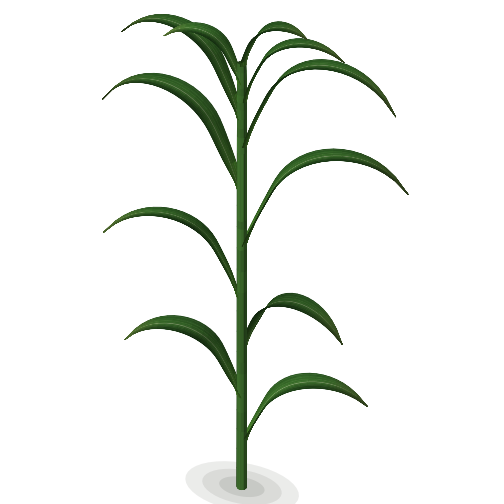
\includegraphics[width=0.8400in, height=0.8400in]{Figures/fig5/maize_plant_0320_90_Ground_truth.png}};
\node[anchor=south west, inner sep=0] at (5.9250,1.9900) {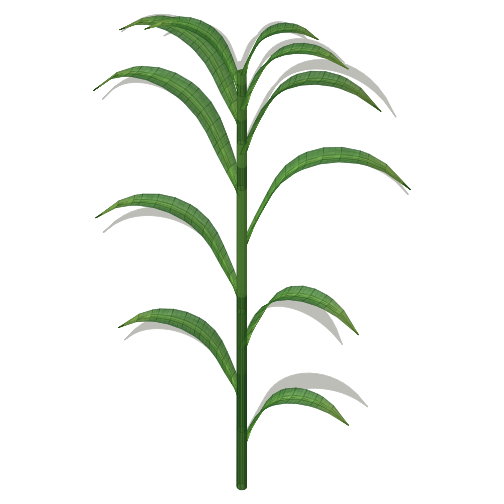
\includegraphics[width=0.8400in, height=0.8400in]{Figures/fig5/maize_plant_0320_90_Row_trained.png}};
\node[anchor=south west, inner sep=0] at (4.0250,1.0200) {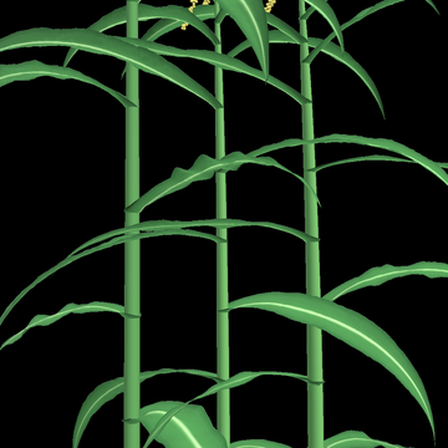
\includegraphics[width=0.8400in, height=0.8400in]{Figures/fig5/maize_plant_6665_0_Row_image.png}};
\node[anchor=south west, inner sep=0] at (4.9750,1.0200) {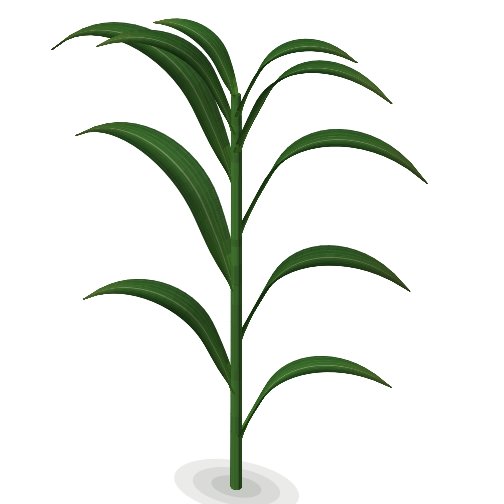
\includegraphics[width=0.8400in, height=0.8400in]{Figures/fig5/maize_plant_6665_0_Ground_truth.png}};
\node[anchor=south west, inner sep=0] at (5.9250,1.0200) {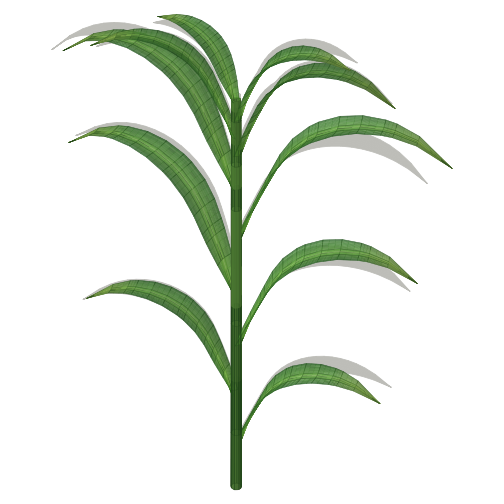
\includegraphics[width=0.8400in, height=0.8400in]{Figures/fig5/maize_plant_6665_0_Row_trained.png}};
\node[anchor=south west, inner sep=0] at (4.0250,0.0500) {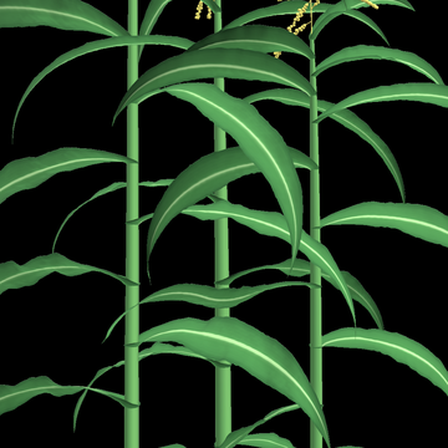
\includegraphics[width=0.8400in, height=0.8400in]{Figures/fig5/maize_plant_4604_0_Row_image.png}};
\node[anchor=south west, inner sep=0] at (4.9750,0.0500) {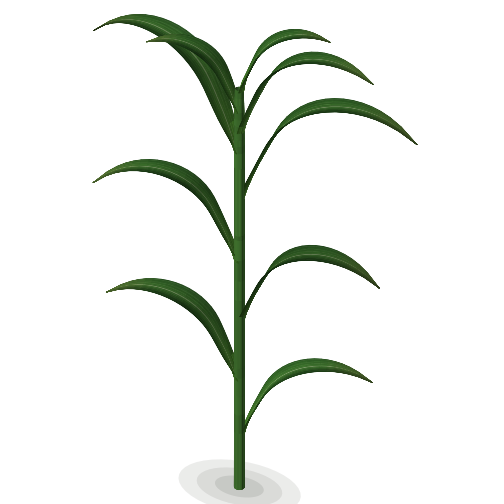
\includegraphics[width=0.8400in, height=0.8400in]{Figures/fig5/maize_plant_4604_0_Ground_truth.png}};
\node[anchor=south west, inner sep=0] at (5.9250,0.0500) {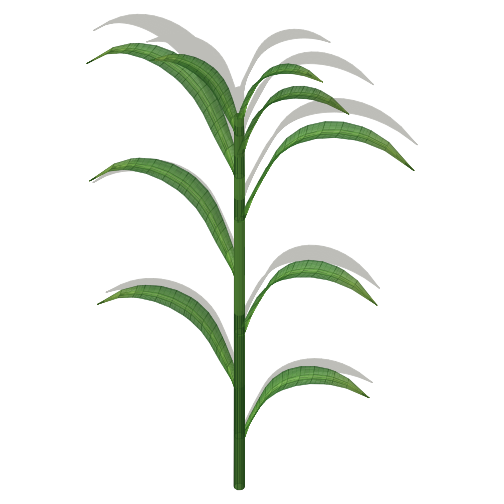
\includegraphics[width=0.8400in, height=0.8400in]{Figures/fig5/maize_plant_4604_0_Row_trained.png}};
\node[anchor=north, inner sep=0, outer sep=0, align=center, text=c1D221C, font={\fontsize{9.00}{11.25}\selectfont\sffamily\bfseries}] at (2.0200,3.3300) {Sorghum};
\node[anchor=north, inner sep=0, outer sep=0, align=center, text=c1A1A1A, font={\fontsize{9.00}{11.25}\selectfont\sffamily}] at (1.0700,3.1400) {Row image};
\node[anchor=north, inner sep=0, outer sep=0, align=center, text=c1A1A1A, font={\fontsize{9.00}{11.25}\selectfont\sffamily}] at (2.0200,3.1400) {Ground truth};
\node[anchor=north, inner sep=0, outer sep=0, align=center, text=c5E4A96, font={\fontsize{9.00}{11.25}\selectfont\sffamily}] at (2.9700,3.1400) {Row-trained};
\node[anchor=south east, inner sep=0, outer sep=0, align=right, text=c5E4A96, font={\fontsize{9.00}{11.25}\selectfont\sffamily}] at (3.3800,2.0000) {MAE = 0.076};
\node[anchor=east, inner sep=0, outer sep=0, align=right, text=c1D221C, font={\fontsize{9.00}{9.90}\selectfont\sffamily}] at (0.5600,2.4100) {Plant\\10756};
\node[anchor=south east, inner sep=0, outer sep=0, align=right, text=c5E4A96, font={\fontsize{9.00}{11.25}\selectfont\sffamily}] at (3.3800,1.0300) {MAE = 0.058};
\node[anchor=east, inner sep=0, outer sep=0, align=right, text=c1D221C, font={\fontsize{9.00}{9.90}\selectfont\sffamily}] at (0.5600,1.4400) {Plant\\14816};
\node[anchor=south east, inner sep=0, outer sep=0, align=right, text=c5E4A96, font={\fontsize{9.00}{11.25}\selectfont\sffamily}] at (3.3800,0.0600) {MAE = 0.071};
\node[anchor=east, inner sep=0, outer sep=0, align=right, text=c1D221C, font={\fontsize{9.00}{9.90}\selectfont\sffamily}] at (0.5600,0.4700) {Plant\\4815};
\node[anchor=north, inner sep=0, outer sep=0, align=center, text=c1D221C, font={\fontsize{9.00}{11.25}\selectfont\sffamily\bfseries}] at (5.3950,3.3300) {Maize};
\node[anchor=north, inner sep=0, outer sep=0, align=center, text=c1A1A1A, font={\fontsize{9.00}{11.25}\selectfont\sffamily}] at (4.4450,3.1400) {Row image};
\node[anchor=north, inner sep=0, outer sep=0, align=center, text=c1A1A1A, font={\fontsize{9.00}{11.25}\selectfont\sffamily}] at (5.3950,3.1400) {Ground truth};
\node[anchor=north, inner sep=0, outer sep=0, align=center, text=c5E4A96, font={\fontsize{9.00}{11.25}\selectfont\sffamily}] at (6.3450,3.1400) {Row-trained};
\node[anchor=south east, inner sep=0, outer sep=0, align=right, text=c5E4A96, font={\fontsize{9.00}{11.25}\selectfont\sffamily}] at (6.7550,2.0000) {MAE = 0.047};
\node[anchor=east, inner sep=0, outer sep=0, align=right, text=c1D221C, font={\fontsize{9.00}{9.90}\selectfont\sffamily}] at (3.9350,2.4100) {Plant\\0320};
\node[anchor=south east, inner sep=0, outer sep=0, align=right, text=c5E4A96, font={\fontsize{9.00}{11.25}\selectfont\sffamily}] at (6.7550,1.0300) {MAE = 0.035};
\node[anchor=east, inner sep=0, outer sep=0, align=right, text=c1D221C, font={\fontsize{9.00}{9.90}\selectfont\sffamily}] at (3.9350,1.4400) {Plant\\6665};
\node[anchor=south east, inner sep=0, outer sep=0, align=right, text=c5E4A96, font={\fontsize{9.00}{11.25}\selectfont\sffamily}] at (6.7550,0.0600) {MAE = 0.038};
\node[anchor=east, inner sep=0, outer sep=0, align=right, text=c1D221C, font={\fontsize{9.00}{9.90}\selectfont\sffamily}] at (3.9350,0.4700) {Plant\\4604};
\end{tikzpicture}%
}%
}
    \vspace{-15pt}

  \caption{\textbf{Reconstructing occluded target plants in simulated crop rows} (held-out sorghum test rows on the left, maize on the right). The columns show the input row photograph (including the adjacent neighbors), the ground-truth procedural model of the center target plant (drawn as a stem-and-leaf schematic), and the procedural model predicted by the row fine-tuned model (purple) over the ground truth (grey). The leaf-parameter MAE (normalized fields, as in \tabref{tab:rows-main}) is noted below each prediction. The examples are selected from plants where the row fine-tuned model ranks in its top 35\% by Chamfer distance and the isolated control ranks in its bottom 40\%, across both broadside and end-on views. \textcolor{cvprblue}{Figs.}~\ref{fig:supp-rows-sorghum} and~\ref{fig:supp-rows-maize} show ten additional test plants per species, sampled evenly across the full error distribution.}
  \label{fig:rowsex}
\end{figure*}

\subsection{Experimental Setup}
\label{sec:setup}\label{sec:exp-setup}

\noindent\textbf{Models.}
All models use a ViT-Base backbone (114\,M parameters). We refer to the Stage~1 model as the \emph{pretrained} model (the headline model in the Appendix), to the Stage~2 generalist student as the \emph{distilled} model, and to the Stage~3 model as the \emph{row fine-tuned} model. The distilled and row fine-tuned models are two separate specializations of the pretrained model, and we train them per species. As a control for Stage~3, we also report an \emph{isolated control} that is trained only on isolated plants. The isolated control starts from the same Stage~1 weights and follows the same schedule as the row fine-tuned model (100 epochs, learning rate $10^{-4}$, global batch size 32, mask ratio 0.8), but its inputs and reconstruction targets are the isolated captures of the same plants.


\noindent\textbf{Metrics.}
The output of interest is the procedural plant, and we therefore score it in parameter space. Additionally, we report the fraction of plants whose predicted leaf count is within one leaf of the ground truth, the relative error in plant height, and the leaf-parameter \emph{skill} ($1 - \mathrm{MAE}/\mathrm{MAE}_{\mathrm{mean}}$, where $0$ matches predicting the dataset mean) or the normalized MAE. For the reconstructed geometry, we report the symmetric squared Chamfer distance and the point-cloud $F_1$ score. Note that Chamfer distance is less informative on thin foliage.
% (\appendixref{sec:exp-metrics}). \textcolor{cvprblue}{Appendices}~\ref{app:metrics}, \ref{app:analyses}, and~\ref{app:tables} give the metric definitions, additional analyses, and full tables.
Please refer to the Appendix for detailed metric definitions, additional analyses, and full tables.

\subsection{Neighbor Occlusion in Crop Rows}
\label{sec:regime3}\label{sec:exp-occlusion}

\begin{table}[t]
  \caption{\textbf{The same test plants in isolation and in simulated crop rows} (2{,}250 test plants per species, ten row orientations). Chamfer distance to the target plant is in $10^{-4}\,\mathrm{m}^2$, and MAE is the leaf-parameter MAE on rows. \tabref{tab:rows} gives all inputs with confidence intervals.}
  \label{tab:rows-main}
  \centering\scriptsize
  \setlength{\tabcolsep}{1.2pt}
\renewcommand{\arraystretch}{1.5}
  \resizebox{\columnwidth}{!}{%
  \begin{tabular}{ll ccc ccc}
    \toprule
    & & \multicolumn{3}{c}{Maize} & \multicolumn{3}{c}{Sorghum} \\
    \cmidrule(lr){3-5}\cmidrule(lr){6-8}
    & & \multicolumn{2}{c}{Chamfer $\downarrow$} & MAE $\downarrow$ & \multicolumn{2}{c}{Chamfer $\downarrow$} & MAE $\downarrow$ \\
    Model & Input & Isolated & Row & Row & Isolated & Row & Row \\
    \midrule
    Isolated control & All & \textbf{1.8} & 29.0 & 0.093 & \textbf{13.1} & 133.8 & 0.096 \\
    Pretrained, zero-shot & All & 26.4 & 29.6 & 0.093 & 174.3 & 230.5 & 0.114 \\
    \midrule
    Row fine-tuned & All & 12.6 & \textbf{4.0} & \textbf{0.052} & 38.7 & 30.7 & 0.061 \\
     & RGB & 13.7 & 14.4 & 0.071 & 34.8 & 29.8 & 0.097 \\
     & Depth & 10.3 & 9.6 & 0.064 & 24.4 & \textbf{18.6} & \textbf{0.055} \\
     & Point cloud & 21.7 & 21.9 & 0.073 & 46.0 & 70.8 & 0.082 \\
    \bottomrule
  \end{tabular}}
\end{table}
% REVIEWER FLAG: bold marks the true best value per column. In Table tab:rows (appendix) the sorghum all-streams entries (30.7, 0.061) are bold although depth-only is lower (18.6, 0.055). Co-authors to check.


\tabref{tab:rows-main} compares the reconstruction of the same test plants in isolation and inside crop rows. The isolated control breaks down under row occlusion. Its Chamfer distance increases by a factor of 16 in maize ($1.8 \to 29.0 \times 10^{-4}\,\mathrm{m}^2$) and by a factor of 10 in sorghum ($13.1 \to 133.8 \times 10^{-4}\,\mathrm{m}^2$), because it reconstructs neighboring foliage as part of the target plant. Fine-tuning on simulated rows removes 92\% of this neighbor-induced error in maize ($29.0 \to 4.0$) and 85\% in sorghum ($133.8 \to 30.7$). The leaf-parameter MAE on rows also falls from 0.093 to 0.052 in maize and from 0.096 to 0.061 in sorghum (\figref{fig:rowsex}). The row fine-tuned model also works from a single sensor, with a leaf-parameter MAE of 0.064 to 0.073 in maize and 0.055 to 0.097 in sorghum.


\noindent\textbf{Occlusion realism.}
We also test whether simpler occlusions suffice for training (see the Appendix). On rendered maize test rows, the $F_1$ at 10\,mm rises from 0.416 (training on isolated plants) to 0.552 (2D B\'ezier leaf occluders), 0.717 (unbent 3D neighbor clouds), and 0.789 (contact-solved rows). \textit{The reconstruction thus improves steadily as the training occlusion approaches the physical rows.}
% APPENDIX REF (removed for submission, restore later): (\appendixref{sec:abl_occ}) (for: see Appendix)

\subsection{Rows Assembled from Real Plants}
\label{sec:res-field}\label{sec:exp-real}


We next evaluate on crop rows built from real plants. We use the procedural models of 520 real maize plants released with MaizeField3D~\citep{maizefield3d2025} and our own laser scans of 30 real sorghum plants (2.2 to 5.3\,m tall). The plants are arranged into rows at 15 to 25\,cm spacing in two orientations and imaged from 18 rover camera stops per row. The sensor streams are rendered with the same pipeline as the training data. This isolates the transfer to real plant morphology from the effect of sensor noise.


% \begin{table}[t]
%   \caption{\textbf{Rows assembled from real plants.} All three sensor streams are given as input. Chamfer is the target distance in $10^{-4}$\,m$^2$ with 95\% bootstrap confidence intervals over plants. Miss@5\,mm is the fraction of ground-truth target points farther than 5\,mm from any predicted point. Height is the median relative height error, and Leaves $\pm 1$ is the share of camera stops whose predicted leaf count is within one leaf of the ground truth (the sorghum scans have no comparable height or leaf-count labels). \emph{Real-row FT} denotes the row fine-tuned model further trained on 75\% of the real plants. On synthetic test rows, the row fine-tuned model reaches 4.0 (maize) and 30.7 (sorghum).}
%   \label{tab:e10}
%   \centering\scriptsize
%   \setlength{\tabcolsep}{1.2pt}
%   \renewcommand{\arraystretch}{1.5}
%   \resizebox{\columnwidth}{!}{%
%   \begin{tabular}{llcccc}
%     \toprule
%     Rows (plants) & Model & Chamfer $\downarrow$ & Miss@5\,mm $\downarrow$ & Height $\downarrow$ & Leaves $\pm1$ $\uparrow$ \\
%     \midrule
%     \multicolumn{6}{l}{\emph{Zero-shot, all real plants}} \\
%     Maize parallel (520) & Pretrained (no row FT) & 75.1 {\tiny[73.1, 77.2]} & 0.92 & 53\% & 17\% \\
%      & Isolated control & 55.6 {\tiny[54.2, 57.2]} & 0.93 & 43\% & 4\% \\
%      & Row fine-tuned (FT) & \textbf{41.2} {\tiny[39.7, 42.8]} & 0.93 & \textbf{37\%} & \textbf{47\%} \\
%     Maize perpend.\ (520) & Pretrained (no row FT) & 121.2 {\tiny[116.6, 127.2]} & 0.96 & 52\% & 23\% \\
%      & Isolated control & 137.3 {\tiny[133.6, 141.9]} & 0.98 & 40\% & 13\% \\
%      & Row fine-tuned (FT) & \textbf{80.0} {\tiny[76.4, 85.2]} & 0.97 & \textbf{35\%} & \textbf{46\%} \\
%     Sorghum, both (30) & Pretrained (no row FT) & 2{,}541 {\tiny[2{,}205, 2{,}886]} & 0.99 & n/a & n/a \\
%      & Isolated control & \textbf{975} {\tiny[876, 1{,}079]} & 0.99 & n/a & n/a \\
%      & Row fine-tuned (FT) & 2{,}145 {\tiny[1{,}910, 2{,}376]} & 0.99 & n/a & n/a \\
%     \midrule
%     \multicolumn{6}{l}{\emph{Fine-tuned on 75\% of the real plants, scored on the held-out 25\%}} \\
%     Maize, both (130) & Row FT & 59.5 {\tiny[56.0, 63.2]} & 0.95 & 36\% & 45\% \\
%      & Real-row FT & \textbf{19.7} {\tiny[18.6, 21.0]} & \textbf{0.87} & \textbf{1.6\%} & \textbf{70\%} \\
%     Sorghum, both (8) & Row FT & 2{,}113 {\tiny[1{,}647, 2{,}520]} & 0.99 & n/a & n/a \\
%      & Real-row FT & \textbf{79.4} {\tiny[68.3, 92.6]} & \textbf{0.92} & n/a & n/a \\
%     \bottomrule
%   \end{tabular}}
% \end{table}

Evaluated zero-shot (\tabref{tab:e10}), the row fine-tuned model outperforms both the pretrained model and the isolated control on both maize row layouts. This indicates that the row-occlusion training transfers to real plant geometry. However, the absolute errors remain roughly an order of magnitude higher than on synthetic rows, due to a size mismatch. 83\% of the real maize plants are taller than the tallest synthetic training plant (1.33\,m), and the median height error is 14\% on in-range plants vs.\ 38\% on taller plants. Similarly, the real sorghum plants (up to 5.3\,m) far exceed the synthetic training range (1.74\,m).


\begin{table}[t]
  % \caption{\textbf{Rows assembled from real plants.} All three sensor streams are given as input. Chamfer is the target distance in $10^{-4}$\,m$^2$ with 95\% bootstrap confidence intervals over plants. Miss@5\,mm is the fraction of ground-truth target points farther than 5\,mm from any predicted point. Height is the median relative height error, and Leaves $\pm 1$ is the share of camera stops whose predicted leaf count is within one leaf of the ground truth (the sorghum scans have no comparable height or leaf-count labels). \emph{Real-row FT} denotes the row fine-tuned model further trained on 75\% of the real plants. On synthetic test rows, the row fine-tuned model reaches 4.0 (maize) and 30.7 (sorghum).}
  \caption{\textbf{Rows assembled from real plants.} All three sensor streams are given as input. Target Chamfer distance ($10^{-4}$\,m$^2$, 95\% plant bootstrap CI), Miss@5\,mm (ground-truth points $>5$\,mm from prediction), median relative height error, and $\pm 1$-leaf accuracy across camera stops. \emph{Real-row FT} denotes the row fine-tuned model trained on 75\% of the real plants. On synthetic test rows, the row fine-tuned model reaches 4.0 (maize) and 30.7 (sorghum).}

  \label{tab:e10}
  \centering\scriptsize
  \setlength{\tabcolsep}{0.5pt}
  \renewcommand{\arraystretch}{1.65}
  \resizebox{\columnwidth}{!}{%
  \begin{tabular}{llcccc}
    \toprule
    Rows (plants) & Model & Chamfer $\downarrow$ & Miss@5\,mm $\downarrow$ & Height $\downarrow$ & Leaves $\pm1$ $\uparrow$ \\
    \midrule
    \multicolumn{6}{l}{\emph{Zero-shot, all real plants}} \\
    Maize parallel (520) & Pretrained (no row FT) & 75.1 {\tiny[73.1, 77.2]} & 0.92 & 53\% & 17\% \\
     & Isolated control & 55.6 {\tiny[54.2, 57.2]} & 0.93 & 43\% & 4\% \\
     & Row fine-tuned (FT) & \textbf{41.2} {\tiny[39.7, 42.8]} & 0.93 & \textbf{37\%} & \textbf{47\%} \\
    Maize perpend.\ (520) & Pretrained (no row FT) & 121.2 {\tiny[116.6, 127.2]} & 0.96 & 52\% & 23\% \\
     & Isolated control & 137.3 {\tiny[133.6, 141.9]} & 0.98 & 40\% & 13\% \\
     & Row fine-tuned (FT) & \textbf{80.0} {\tiny[76.4, 85.2]} & 0.97 & \textbf{35\%} & \textbf{45\%} \\
    Sorghum, both (30) & Pretrained (no row FT) & 2{,}541 {\tiny[2{,}205, 2{,}886]} & 0.99 & \textbf{77\%} & \textbf{37\%} \\
     & Isolated control & \textbf{975} {\tiny[876, 1{,}079]} & 0.99 & 81\% & 19\% \\
     & Row fine-tuned (FT) & 2{,}145 {\tiny[1{,}910, 2{,}376]} & 0.99 & 86\% & 20\% \\
    \midrule
    \multicolumn{6}{l}{\emph{Fine-tuned on 75\% of the real plants, scored on the held-out 25\%}} \\
    Maize, both (130) & Row FT & 59.5 {\tiny[56.0, 63.2]} & 0.95 & 36\% & 45\% \\
     & Real-row FT & \textbf{19.7} {\tiny[18.6, 21.0]} & \textbf{0.87} & \textbf{1.6\%} & \textbf{70\%} \\
    Sorghum, both (8) & Row FT & 2{,}113 {\tiny[1{,}647, 2{,}520]} & 0.99 & 86\% & 17\% \\
     & Real-row FT & \textbf{79.4} {\tiny[68.3, 92.6]} & \textbf{0.92} & \textbf{74\%} & \textbf{49\%} \\
    \bottomrule
  \end{tabular}}
\end{table}


Fine-tuning the row model for 15 epochs on the real plants (split by plant) closes most of this gap on the held-out (130 maize and 8 sorghum) plants. The median maize height error drops from 36\% to 1.6\%, and the leaf count accuracy within one leaf rises from 45\% to 70\%. The Chamfer distance falls from 59.5 to $19.7 \times 10^{-4}\,\mathrm{m}^2$ in maize and from 2{,}113 to $79.4 \times 10^{-4}\,\mathrm{m}^2$ in sorghum. These improvements hold across single-sensor and multi-sensor inputs, row layouts, and plant heights (see the Appendix). Inference takes 10.6\,ms per camera stop. %\textcolor{red}{[Pointer to the in-field result in the appendix, once available.]}
% APPENDIX REF (removed for submission, restore later): (\tabref{tab:e10_detail}, \appendixref{app:tables}) (for: see the Appendix)


\subsection{Single-Sensor Reconstruction of Isolated Plants}
\label{sec:regime1}\label{sec:exp-regime1}\label{sec:res-distill}\label{sec:exp-main}

% \begin{table}[!h]
%   \caption{\textbf{Single-sensor reconstruction of isolated plants} (2{,}250 validation plants per species). Leaf count is the fraction of plants within one leaf of the ground truth, height is the relative error, and leaf skill is Eq.~\eqref{eq:trait-skill} averaged over the leaf parameters. $F_1$ (at $\tau = 0.01$) and Chamfer distance ($\times 10^{-3}$) are computed in the unit-sphere frame. The two-stage variant routes the model through its own generated cloud (RGB to cloud, then cloud to parameters). \tabref{tab:regime1} gives the full results.}
%   \label{tab:single}
%   \centering\scriptsize
%   \setlength{\tabcolsep}{0.7pt}
%   \renewcommand{\arraystretch}{1.5}
%   \resizebox{\columnwidth}{!}{%
%   \begin{tabular}{l ccc cc}
%     \toprule
%     Input & Leaf count $\pm1$ $\uparrow$ & Height err.\ $\downarrow$ & Leaf skill $\uparrow$ & $F_1$ $\uparrow$ & Chamfer $\downarrow$ \\
%     \midrule
%     \multicolumn{6}{l}{\emph{Sorghum}} \\
%     RGB & 0.909 & 0.036 & 0.656 & 0.386 & 1.36 \\
%     Depth & 0.956 & 0.026 & \textbf{0.679} & \textbf{0.440} & \textbf{0.93} \\
%     Point cloud & \textbf{0.998} & \textbf{0.022} & 0.675 & 0.370 & 1.45 \\
%     Two-stage: RGB $\to$ cloud $\to$ $\theta$ & 0.301 & 0.221 & $-0.010$ & 0.386 & 1.36 \\
%     \midrule
%     \multicolumn{6}{l}{\emph{Maize}} \\
%     RGB & 0.973 & 0.045 & 0.567 & 0.482 & 0.83 \\
%     Depth & 0.972 & 0.046 & 0.571 & \textbf{0.529} & \textbf{0.64} \\
%     Point cloud & \textbf{0.986} & \textbf{0.043} & \textbf{0.587} & 0.455 & 0.87 \\
%     Two-stage: RGB $\to$ cloud $\to$ $\theta$ & 0.066 & 0.131 & 0.015 & 0.482 & 0.83 \\
%     \bottomrule
%   \end{tabular}}
% \end{table}

We next examine the single-sensor specialization on isolated validation plants (\tabref{tab:single}). For all three inputs, the predicted leaf count is within one leaf of the ground truth on 91 to 100\% of plants, the height error is 2 to 5\%, and the mean leaf-parameter skill is 0.66 to 0.68 in sorghum and 0.57 to 0.59 in maize.

\begin{table}[H]
  \caption{\textbf{Single-sensor reconstruction of isolated plants} (2{,}250 validation plants per species). Leaf count is the fraction of plants within one leaf of the ground truth, height is the relative error, and leaf skill is Eq.~\eqref{eq:trait-skill} averaged over the leaf parameters. $F_1$ (at $\tau = 0.01$) and Chamfer distance ($\times 10^{-3}$) are computed in the unit-sphere frame. The two-stage variant routes the model through its own generated cloud (RGB to cloud, then cloud to parameters). \tabref{tab:regime1} gives the full results.}
  \label{tab:single}
  \centering\scriptsize
  \setlength{\tabcolsep}{0.7pt}
  \renewcommand{\arraystretch}{1.5}
  \resizebox{\columnwidth}{!}{%
  \begin{tabular}{l ccc cc}
    \toprule
    Input & Leaf count $\pm1$ $\uparrow$ & Height err.\ $\downarrow$ & Leaf skill $\uparrow$ & $F_1$ $\uparrow$ & Chamfer $\downarrow$ \\
    \midrule
    \multicolumn{6}{l}{\emph{Sorghum}} \\
    RGB & 0.909 & 0.036 & 0.656 & 0.386 & 1.36 \\
    Depth & 0.956 & 0.026 & \textbf{0.679} & \textbf{0.440} & \textbf{0.93} \\
    Point cloud & \textbf{0.998} & \textbf{0.022} & 0.675 & 0.370 & 1.45 \\
    Two-stage: RGB $\to$ cloud $\to$ $\theta$ & 0.301 & 0.221 & $-0.010$ & 0.386 & 1.36 \\
    \midrule
    \multicolumn{6}{l}{\emph{Maize}} \\
    RGB & 0.973 & 0.045 & 0.567 & 0.482 & 0.83 \\
    Depth & 0.972 & 0.046 & 0.571 & \textbf{0.529} & \textbf{0.64} \\
    Point cloud & \textbf{0.986} & \textbf{0.043} & \textbf{0.587} & 0.455 & 0.87 \\
    Two-stage: RGB $\to$ cloud $\to$ $\theta$ & 0.066 & 0.131 & 0.015 & 0.482 & 0.83 \\
    \bottomrule
  \end{tabular}}
\end{table}


\noindent\textbf{Direct prediction vs.\ routing through a point cloud.}
A natural alternative is to reconstruct the geometry first and to read the parameters from it. As an ablation, we route our own model through its generated cloud (RGB to cloud, then cloud to parameters). This two-stage variant loses almost all parameter accuracy. The leaf count accuracy falls from 91\% to 30\% in sorghum and from 97\% to 7\% in maize, and the sorghum leaf skill drops from 0.66 to $-0.01$. This indicates that the parameters should be predicted directly from the sensor data.
% REVIEWER FLAG (V3): the two-stage result is now presented as an ablation of our own model (the cloud F1 and Chamfer are identical to the RGB row, so stage one is our model). Co-authors to confirm that stage two is also our model's cloud-to-parameter path.

\noindent\textbf{All-modality training improves every sensor.}
Distillation from the full-modality teacher improves all single-sensor conversions (see the tables in the Appendix).%\tabref{tab:main}, \appendixref{app:tables}
% APPENDIX REF (removed for submission, restore later): (\tabref{tab:main}, \appendixref{app:tables}) (for: see table in the Appendix)
The mean cross-modal generation loss falls by 30.2\% in sorghum and 43.5\% in maize. The gains are largest on the hardest conversions. In sorghum, the RGB-to-parameter MAE drops by 76\% ($0.058 \to 0.014$), the point-cloud-to-parameter MAE is halved ($0.040 \to 0.020$), and the RGB-to-cloud Chamfer distance improves by 61\% ($2.27 \to 0.88 \times 10^{-3}$). Reconstructing all streams also helps the parameters themselves. On complete validation point clouds, the distilled generalist outperforms a specialist student trained only to regress parameters from the same initialization (parameter MAE of 0.019 vs.\ 0.036).
% REVIEWER FLAG: 0.019 (specialist comparison, complete clouds) vs. 0.020 (Table tab:anysubset, random views) for the sorghum point-cloud entry. Both are kept with their evaluation stated. Co-authors to confirm the two evaluations differ.

\noindent\textbf{Comparison with published encoders.}
\tabref{tab:baselines-main} compares the frozen \method{} encoder against DINOv2, MultiMAE, Point-MAE, and EmbodiedMAE under an identical linear-probe protocol~\citep{chen2020simclr}. The pretrained \method{} encoder gives the highest $R^2$ on all probed traits in both species, with the largest margin in maize. Note that these encoders do not output a procedural model, and the comparison is thus at the level of the learned representation.

\begin{table}[t]
  \caption{\textbf{Linear probes on frozen published encoders} (validation $R^2$, higher is better). Each encoder receives the modalities it was designed for. \tabref{tab:baselines} lists all probed traits.}
  \label{tab:baselines-main}
  \centering\scriptsize
  \setlength{\tabcolsep}{0.5pt}
  \renewcommand{\arraystretch}{1.6}
  \resizebox{\columnwidth}{!}{%
  \begin{tabular}{l ccc cccc}
    \toprule
    & \multicolumn{3}{c}{Sorghum} & \multicolumn{4}{c}{Maize} \\
    \cmidrule(lr){2-4}\cmidrule(lr){5-8}
    Frozen encoder & Height & Roll & Leaf len. & Height & Leaf angle & Curl & Stem rad. \\
    \midrule
    DINOv2 (RGB)~\cite{oquab2024dinov2} & 0.924 & 0.573 & 0.235 & 0.561 & 0.816 & 0.072 & 0.588 \\
    MultiMAE (RGB+D)~\cite{bachmann2022multimae} & 0.922 & 0.679 & 0.232 & 0.570 & 0.783 & 0.069 & 0.442 \\
    Point-MAE (PC)~\cite{pang2022pointmae} & 0.958 & 0.716 & 0.188 & 0.509 & 0.863 & 0.199 & 0.426 \\
    EmbodiedMAE (RGB+D+PC)~\cite{dong2025embodiedmae} & 0.976 & 0.765 & 0.265 & 0.528 & 0.823 & 0.139 & 0.428 \\
    \method{} (ours) & \textbf{0.983} & \textbf{0.798} & \textbf{0.371} & \textbf{0.747} & \textbf{0.967} & \textbf{0.739} & \textbf{0.841} \\
    \bottomrule
  \end{tabular}}
\end{table}

% \subsection{Analysis}
% \label{sec:exp-analysis}

\noindent\textbf{Parameters as conditioning.}
The procedural parameters are the output at inference. However, the parameter stream is also an input during pretraining, and known parameters can thus be supplied as a prior. Giving the parameters together with an RGB image reduces the cloud Chamfer distance from 0.88 to 0.39 in sorghum and from 0.77 to 0.41 in maize ($\times 10^{-3}$, \tabref{tab:main}). This suggests a simple route for injecting prior knowledge (such as the growth stage) into the reconstruction.
Please see the Appendix for an analysis of the effect of parameter-token visibility on the sensor representations learned during pretraining.
% APPENDIX REF (removed for submission, restore later): \appendixref{sec:exp-params} (for: Please see Appendix for an analysis ...)
%\appendixref{sec:exp-params} analyzes how the visibility of the parameter tokens during pretraining affects the sensor representations.
% REVIEWER FLAG: the conditioning result uses the full parameter vector. A partial prior (plant-level token only, e.g. leaf count) has not been tested. This is an inference-only experiment on the existing model if co-authors want to add it.
% \appendixref{app:analyses} gives further analyses.
% APPENDIX REF (removed for submission, restore later): \appendixref{app:analyses} gives further analyses. (sentence removed; was the last line of the Experiments section)

%%%%%%%%%%%%%%%%%%%%%%%%%%%%%%%%%%%%%%%%%%%%%%%%%%%%%%%%%%%%%%%%%%%%%%%%%%%
% 5. LIMITATIONS AND CONCLUSION
%%%%%%%%%%%%%%%%%%%%%%%%%%%%%%%%%%%%%%%%%%%%%%%%%%%%%%%%%%%%%%%%%%%%%%%%%%%
\section{Limitations and Conclusions}
\label{sec:discussion}\label{sec:conclusion}

We note the following \noindent\textbf{limitations}: (a) the sensor inputs in all experiments are rendered, including those for the rows assembled from real plants, and evaluation on real sensor captures is left as future work; (b) the recovered model is bounded by the expressivity of the generator $G$, and anomalies absent from $G$ are projected onto the nearest valid procedural configuration; (c) transfer to plants outside the synthetic size range requires improving the synthetic model or fine-tuning on real plants. %and (d) the ablations use a single random seed per arm.
%

\noindent\textbf{Conclusions.}
We presented \method{}, which recovers complete, editable procedural plant models from any subset of RGB, depth, and point-cloud inputs in milliseconds. The key idea is to use the procedural generator as both the training data and the output space, with one multimodal pretraining and two specializations (single-sensor distillation and row-occlusion fine-tuning). We envision \method{} as a step towards field-scale digital assets for breeding and precision agriculture.

% =========================================================================
% REFERENCES
% =========================================================================
\clearpage % references start on a new page (page 9)


\section*{LLM Usage Statement}
Large language models (Anthropic Claude Opus 5.5, OpenAI ChatGPT, and Google Gemini) were used to support the development and preparation of this work, including debugging baseline training code, optimizing data-loading scripts, assisting with figure editing and improving manuscript clarity and grammar. Any AI-assisted code was reviewed and validated through unit tests, numerical checks, and empirical comparisons with established baselines. The experimental design was developed by the authors, who take full responsibility for the correctness of the manuscript, experimental results, and codebase.

{
\small
\bibliographystyle{ieeenat_fullname}
\bibliography{CVPR}
}

% =========================================================================
% SUPPLEMENTARY MATERIAL
% =========================================================================
\appendix
\maketitlesupplementary % new page with the paper title and "Supplementary Material" (cvpr.sty)
% Number supplementary figures and tables S1, S2, ...
\setcounter{figure}{0}
\setcounter{table}{0}
\renewcommand{\thefigure}{S\arabic{figure}}
\renewcommand{\thetable}{S\arabic{table}}
\renewcommand{\theHfigure}{S\arabic{figure}}% unique hyperref anchors
\renewcommand{\theHtable}{S\arabic{table}}
%%%%%%%%%%%%%%%%%%%%%%%%%%%%%%%%%%%%%%%%%%%%%%%%%%%%%%%%%%%%%%%%%%%%%%%%%%%
% APPENDIX J: ADDITIONAL ANALYSES (moved verbatim from the main body of the earlier draft)
%%%%%%%%%%%%%%%%%%%%%%%%%%%%%%%%%%%%%%%%%%%%%%%%%%%%%%%%%%%%%%%%%%%%%%%%%%%
\makeatletter
\setlength{\@fptop}{0pt}\setlength{\@fpbot}{0pt plus 1fil}
\setlength{\@dblfptop}{0pt}\setlength{\@dblfpbot}{0pt plus 1fil}
\makeatother

\section{Additional Analyses}
\label{app:analyses}

This appendix collects analyses that support the main paper. We cover (a) the effects of viewpoint, self-occlusion, and plant complexity, (b) the placement of the procedural parameter stream, (c) the relation between Chamfer distance and trait probes, and (d) representation quality and scaling.
% The figures and tables referenced here appear in \textcolor{cvprblue}{Appendices}~\ref{app:figures} and~\ref{app:tables}.
% REVIEWER FLAG: the four subsections below are moved verbatim from the main body of the earlier draft (old Secs. 4.3, 4.6, 4.7, 4.9) and have not yet had the style pass. One change: "monotonically reduces Chamfer distance" now reads "reduces", since Table tab:scaling_ablations is not monotonic (2.48 then 2.53 in sorghum; 0.87 then 0.99 in maize).

\subsection{Viewpoint Elevation, Self-Occlusion, and Complexity}
\label{sec:regime2}\label{sec:exp-regime2}

\noindent\textbf{Effect of camera elevation.}
The ten views of a plant share the same ground-truth procedural parameters, and evaluating across the elevation ladder thus isolates the effect of the camera angle. \subfigref{fig:views}{A} shows that the single-image reconstruction error follows a symmetric U-shaped curve across elevation, with the lowest error for horizontal side views and the highest error when looking steeply down or up. Camera elevation accounts for $\eta^2 = 0.24$ to $0.31$ of the per-plant variance, whereas the morphological traits correlate negligibly with the error ($|\rho| \le 0.06$). Distillation reduces the error by 28\% across all viewpoints, and the U-shaped difficulty profile is preserved. \figref{fig:qual} shows single-photograph reconstructions before and after distillation.

\begin{figure*}[t!]
  \centering
  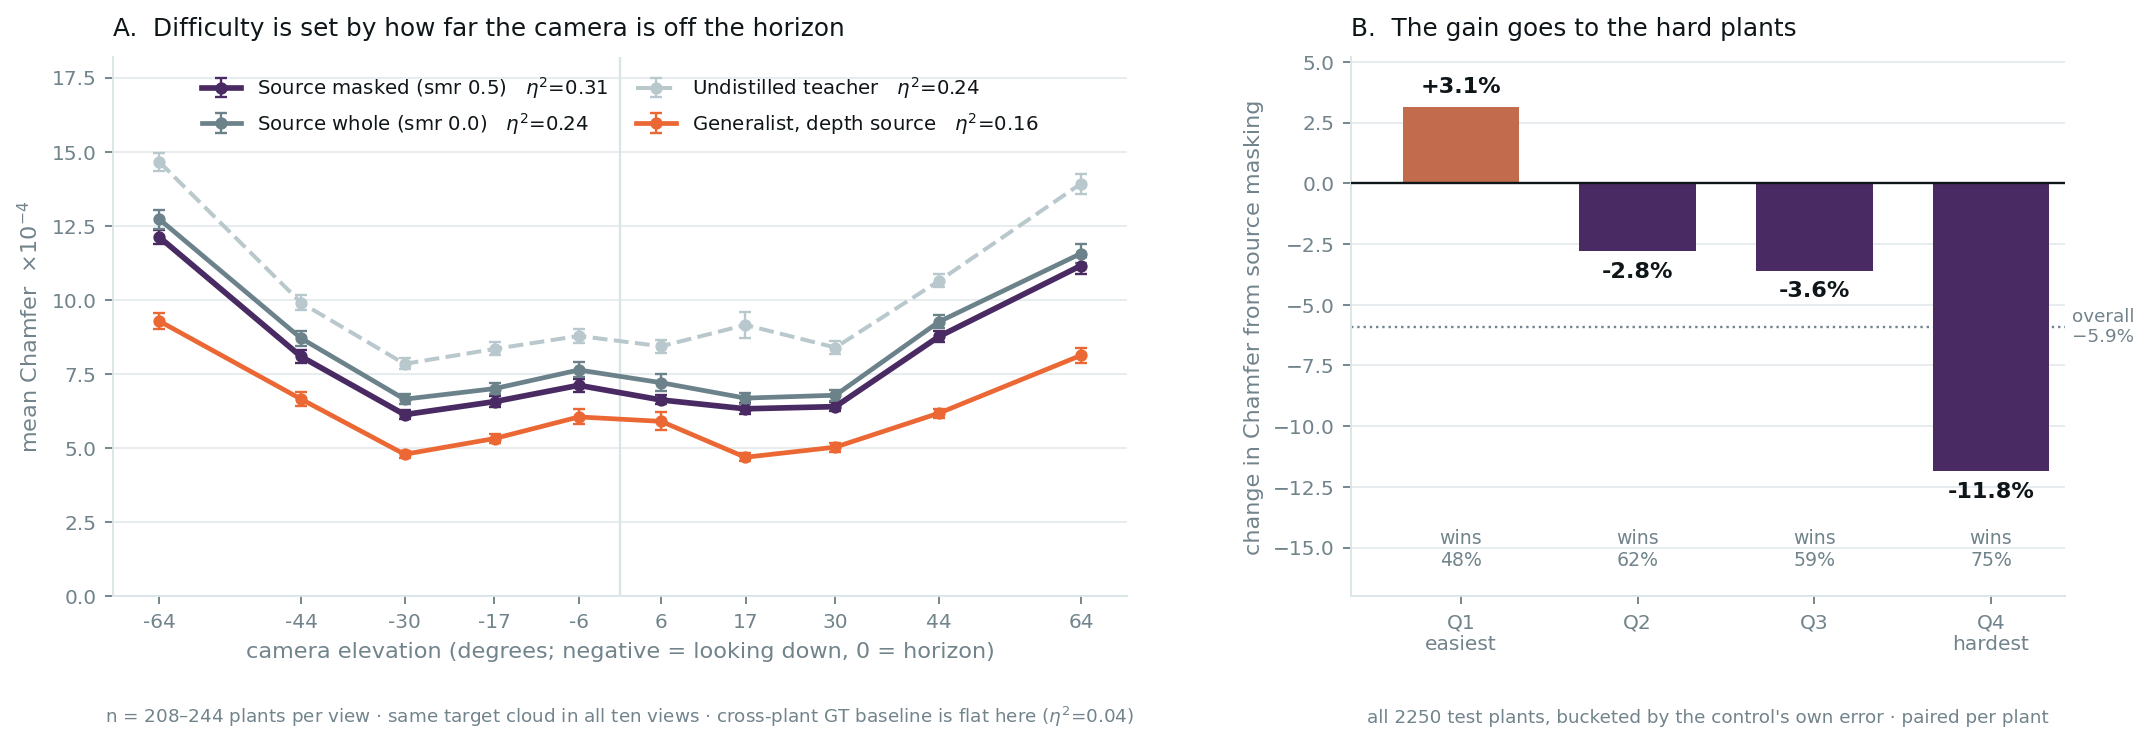
\includegraphics[width=\linewidth]{Figures/fig_view_elevation.png}
  \caption{\textbf{Camera elevation governs single-view reconstruction difficulty.} \textbf{(A)} Photograph-to-cloud Chamfer distance on test plants across camera elevation angles (208 to 244 plants per bin). Both the pretrained and the distilled models follow a symmetric U-shaped curve. They perform best on side views and worst on steep top-down or bottom-up views ($\eta^2 = 0.24$ to $0.31$). \textbf{(B)} Error reduction from masking 50\% of the source tokens during distillation, across baseline error quartiles. The gains are largest on difficult plant geometries.}
  \label{fig:views}
\end{figure*}


\begin{figure*}[t]
  \centering
  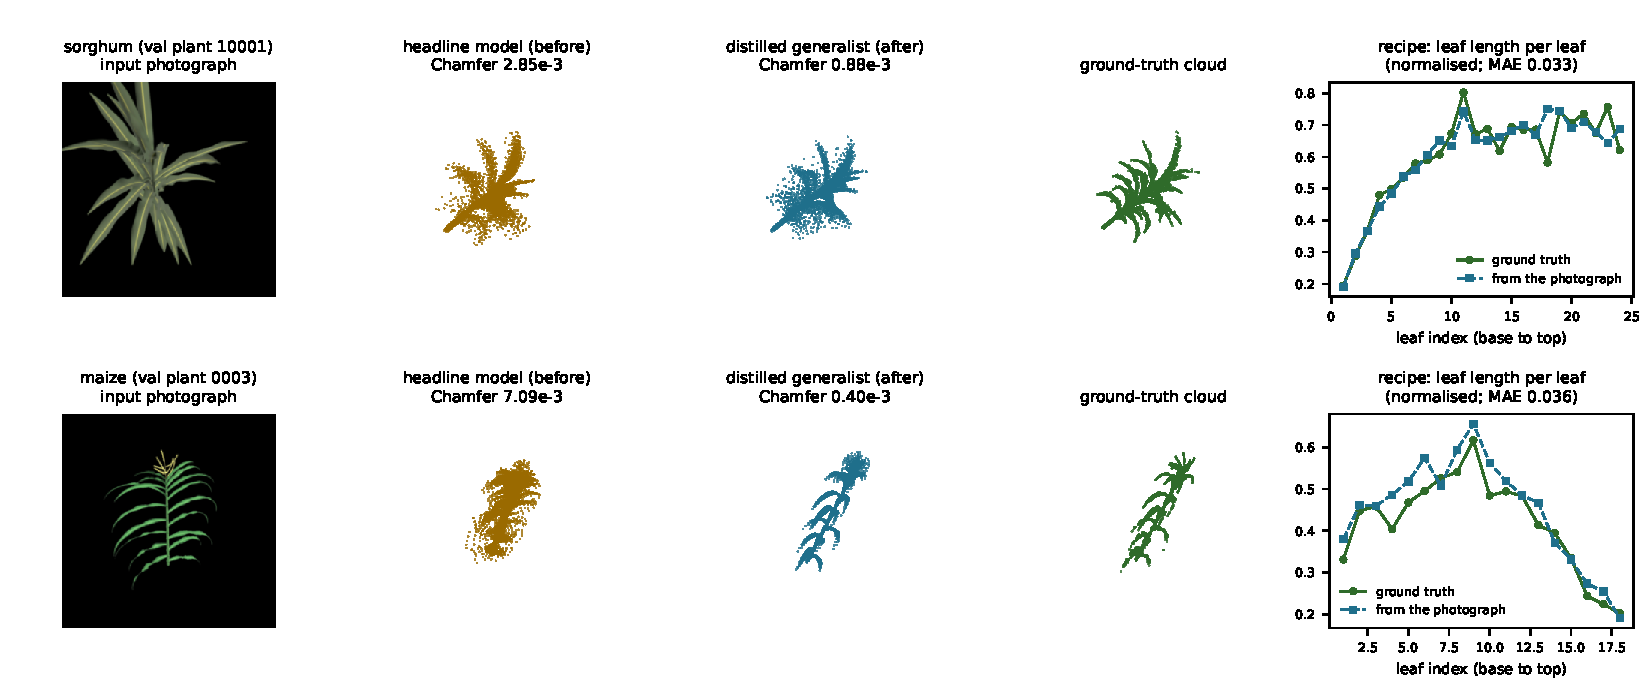
\includegraphics[width=\linewidth]{Figures/fig_qual.pdf}
  \caption{\textbf{Single-photograph 3D reconstruction on held-out test plants.} Each row shows the inference from a single input RGB image (left). Compared to the undistilled headline model, the distilled generalist resolves individual leaf blades and lowers the Chamfer distance (shown above each cloud). The rightmost column compares the normalized leaf lengths predicted by the generalist against the ground truth, from base to top.}
  \label{fig:qual}
\end{figure*}

\noindent\textbf{Training view distribution.}
We pretrain models on narrow elevation bands (top-down views $i \in \{0,1\}$, horizontal views $i \in \{4,5\}$, or a single top-down view $i=0$) and compare them with a model trained on all ten views (\figref{fig:e5views}). The restricted models perform well only at their trained angles and degrade sharply elsewhere. In sorghum, the per-view probe $R^2$ drops by 0.066 to 0.144 on unseen elevations, whereas training across all ten views maintains $R^2 = 0.734$ to $0.778$ at all elevations. In maize, the restricted-view models each lose on 10 to 11 of 11 traits under paired bootstraps, and the point-cloud $F_1$ shows the same pattern. This indicates that covering the full range of evaluation elevations matters far more than the image count alone (\appendixref{app:views-full}).

\begin{figure}[!t]
  \centering
  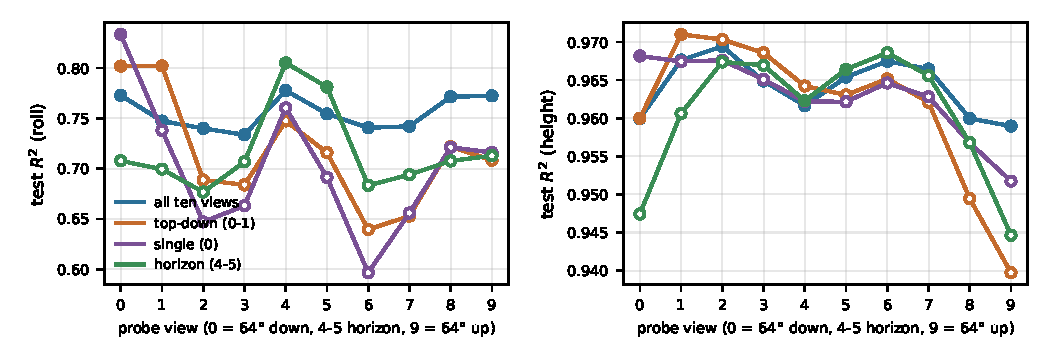
\includegraphics[width=\linewidth]{Figures/fig_e5_views.pdf}
  \caption{\textbf{Impact of training view distribution on downstream trait probing (sorghum test set).} We fit and evaluate the probes per elevation view $k$, for models trained on all ten views and for models trained on restricted elevation bands (filled markers denote the training elevations). Narrow-band training improves the accuracy within the seen elevation range but degrades the generalization to unseen camera angles.}
  \label{fig:e5views}
\end{figure}

\begin{figure}[t]
  \centering
  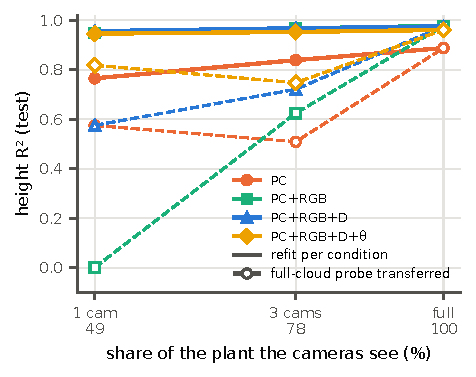
\includegraphics[width=0.95\linewidth]{Figures/fig_partial_clouds.pdf}
  \caption{\textbf{Persistence of phenotypic information under partial surface coverage.} Test-set height $R^2$ plotted against the visible surface percentage for 1-camera, 3-camera, and full coverage. Refitting the linear probe per visibility level (solid lines) preserves high accuracy. In contrast, directly transferring a probe trained on complete clouds (dashed lines) fails due to latent covariate shift.}
  \label{fig:partial}
\end{figure}

\begin{figure}[!t]
  \centering
  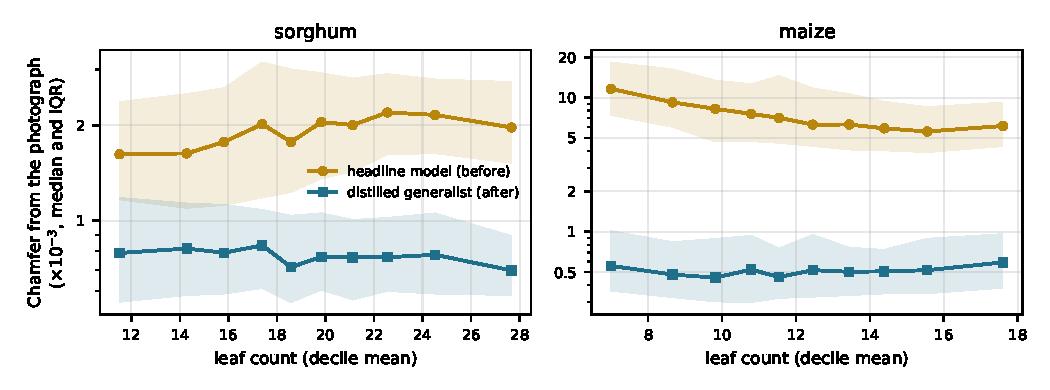
\includegraphics[width=\linewidth]{Figures/fig_leafcount.pdf}
  \caption{\textbf{Reconstruction error across morphological complexity (test set, 2{,}250 plants per species).} Single-photograph Chamfer distance across leaf-count deciles, before and after distillation. After distillation, the error remains flat across the levels of canopy complexity.}
  \label{fig:leafcount}
\end{figure}
% REVIEWER FLAG: "showing that the method scales gracefully to complex canopies" softened to "This suggests that ... scales to plants with complex canopies".



\begin{figure*}[t]
  \centering
  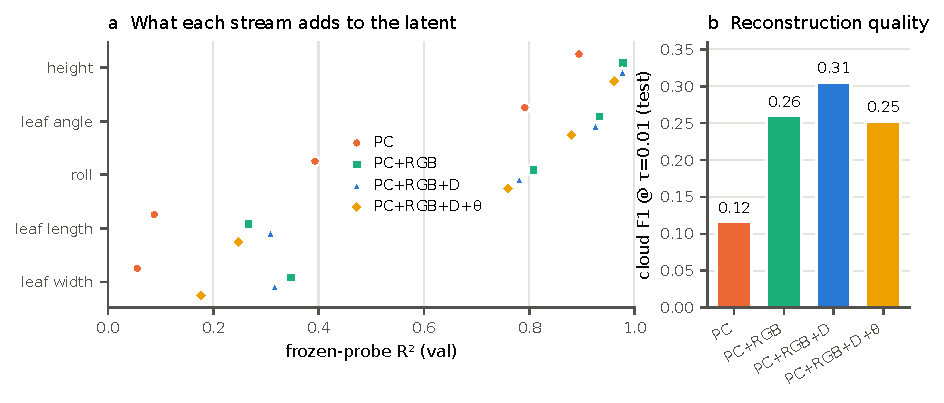
\includegraphics[width=0.8\linewidth]{Figures/fig_e2_streams.pdf}
  \caption{\textbf{Modality contributions to latent representations and geometric reconstruction (sorghum).} \textbf{(a)} Frozen-probe $R^2$ across morphological traits. \textbf{(b)} Point-cloud reconstruction $F_1$ score at threshold $\tau = 0.01$ ($\approx 1$\,cm).}
  \label{fig:stream_contributions}
\end{figure*}

\begin{figure}[t]
  \centering
  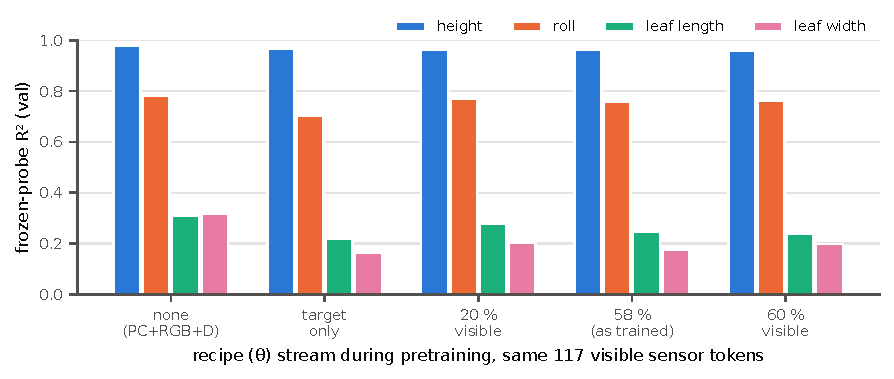
\includegraphics[width=\linewidth]{Figures/fig_param_controls.pdf}
  \caption{\textbf{Effect of procedural parameter visibility during pretraining.} Linear probe $R^2$ across parameter visibility levels under matched sensor token budgets (117.0 visible sensor tokens).}
  \label{fig:controls}
\end{figure}
% REVIEWER FLAG: the opening claim is softened. "Exposing procedural parameter tokens to the encoder degrades sensor representations in both species" now reads "In our experiments, exposing a large fraction of ...", since in Table tab:token_budget the maize arm with 20% visibility improves the probes (height 0.633 to 0.704) and only the 60% arm degrades them (0.521).
% REVIEWER FLAG: the maize height R^2 of 0.776 is the decoder-target-only arm. The gated 20% arm gives 0.704 (Table tab:token_budget). The parenthetical is kept as in the source and does not say which arm it refers to.

\noindent\textbf{Self-occlusion under partial coverage.}
We restrict the point clouds via mesh ray-casting to the surfaces visible from 1 or 3 cameras (49\% and 78\% surface coverage). The latent trait information remains intact if the linear probe is refit to the partial distribution, and the headline model then achieves a height $R^2$ of 0.960 from a single camera. However, a probe trained on 100\% complete clouds fails when it is applied to the single-camera clouds of the same model ($R^2 \to -0.26$, \figref{fig:partial}, \tabref{tab:views}). This indicates that partial visibility induces a systematic covariate shift in the latent space, and field readouts must thus be calibrated on sensor-matched coverage.



\begin{table*}[t]
  \caption{\textbf{Self-occlusion under partial camera coverage (sorghum test set).} We evaluate on point clouds that are restricted via mesh ray-casting to the points visible from 1 or 3 cameras. \emph{Matched} denotes a linear probe that is refit per visibility condition. \emph{Transferred} denotes a linear probe that is fit on 100\% complete clouds and applied without recalibration. Chamfer distance is evaluated against the complete ground-truth cloud. The maize point clouds are single-view captures, and the maize model is thus trained on the 1-camera condition. Its transferred probe is fit on this condition and evaluated on multi-view fused clouds, and its Chamfer distance is measured against the 10-camera validation cloud.}
  \label{tab:views}
  \centering\scriptsize
  \setlength{\tabcolsep}{3.4pt}
  \begin{tabular}{l ccc ccc ccc}
    \toprule
    & \multicolumn{3}{c}{Matched Probe ($R^2$, Height)} & \multicolumn{3}{c}{Transferred Probe ($R^2$, Height)} & \multicolumn{3}{c}{Chamfer ($\times10^{-3}$)} \\
    \cmidrule(lr){2-4}\cmidrule(lr){5-7}\cmidrule(lr){8-10}
    Input Modality & Full & 3-Cam & 1-Cam & Full & 3-Cam & 1-Cam & Full & 3-Cam & 1-Cam \\
    Cloud Coverage & 100\% & 78\% & 49\% & 100\% & 78\% & 49\% & 100\% & 78\% & 49\% \\
    \midrule
    Point Cloud (PC) & 0.888 & 0.839 & 0.765 & 0.888 & 0.509 & 0.575 & 4.99 & 6.18 & 12.8 \\
    $\mathrm{PC}+\mathrm{RGB}$ & 0.977 & 0.967 & 0.948 & 0.977 & 0.624 & 0.001 & 2.49 & 3.64 & 11.5 \\
    $\mathrm{PC}+\mathrm{RGB}+\mathrm{D}$ & 0.975 & 0.968 & 0.956 & 0.975 & 0.721 & 0.576 & 1.76 & 3.06 & 11.4 \\
    Four-Stream Model & 0.961 & 0.953 & 0.946 & 0.961 & 0.748 & 0.818 & 2.52 & 3.62 & 11.4 \\
    Headline Teacher & \textbf{0.982} & \textbf{0.975} & \textbf{0.960} & \textbf{0.982} & 0.623 & $-0.26$ & \textbf{1.36} & 3.14 & 11.6 \\
    \midrule
    \multicolumn{10}{l}{\emph{Maize: Full = 10 cameras fused; coverage 100 / 96 / 72\% of the 10-camera cloud}} \\
    Headline Teacher & 0.719 & 0.698 & 0.754 & 0.108 & 0.251 & 0.754 & 4.98 & 4.54 & 1.15 \\
    \bottomrule
  \end{tabular}
\end{table*}
% REVIEWER FLAG: "fails completely" now reads "fails", and the failure is scoped to the headline model on single-camera clouds. In Table tab:views the transferred 1-camera height R^2 is -0.26 for the headline model only (0.001 to 0.818 for the other four models).

\noindent\textbf{Morphological complexity.}
After distillation, the single-image reconstruction error does not depend on the number of leaves. The error is flat across leaf-count deciles (Spearman $\rho = -0.07$ in sorghum and $+0.04$ in maize, \figref{fig:leafcount}). This suggests that \method{} scales to plants with complex canopies.



\subsection{Influence of Procedural Parameter Stream Placement}
\label{sec:param-stream}\label{sec:exp-params}

\textcolor{cvprblue}{Tables}~\ref{tab:modality_value_add} and~\ref{tab:token_budget} (\appendixref{app:tables}) report how the active input modalities and the visibility of the parameter stream affect the learned encoder representation. The visual streams provide the primary morphological signal. Adding RGB or depth to point clouds lifts the sorghum height $R^2$ from 0.895 to 0.979 and 0.976, and adding RGB lifts the maize height $R^2$ from 0.171 to 0.620. In contrast, depth improves the Chamfer distance by 25 to 28\% but yields almost no gain in the frozen-probe $R^2$.

\begin{table*}[t]
  \caption{\textbf{Controlled ablations under a shared compute budget (197{,}400 optimizer steps).} \textbf{(a) Modality value-add:} We compare the combinations of active input streams. Here, $\theta$ denotes procedural parameter tokens that are included in the shared Dirichlet visibility budget. \textbf{(b) Dataset scale and encoder capacity:} Under a fixed number of gradient steps, larger backbones do not improve the representation quality, while increasing the plant diversity steadily reduces the reconstruction error. We show the validation Chamfer distance ($\times 10^{-3}$) and the linear-probe $R^2$.}
  \label{tab:e2}\label{tab:modality_value_add}\label{tab:scaling}\label{tab:scaling_ablations}
  % REVIEWER FLAG: caption claims kept as written, but panel (b) is not monotone: Chamfer rises from 10{,}000 to 10{,}500 plants (2.48 to 2.53 sorghum, 0.87 to 0.99 maize), and ViT-Base beats ViT-Small on all maize columns. Co-authors to check "steadily" and "larger backbones do not improve".
  \centering\scriptsize
  \begin{minipage}[t]{0.52\textwidth}
    \centering
    \textbf{(a) Modality value-add}\\[3pt]
    \setlength{\tabcolsep}{3.2pt}
    \resizebox{\linewidth}{!}{%
    \begin{tabular}{l c cccccc}
    \toprule
    & Chamfer & \multicolumn{6}{c}{Frozen-Probe $R^2$ (Validation Set)} \\
    \cmidrule(lr){3-8}
    Stream Set & $\times10^{-3}$ & Height & Leaf Cnt & Biomass & Branch & Roll & Leaf Len \\
    \midrule
    \multicolumn{8}{l}{\emph{Sorghum}} \\
    PC & 5.00 & 0.895 & 0.896 & 0.892 & 0.792 & 0.393 & 0.088 \\
    $\mathrm{PC}+\mathrm{D}$ & 2.45 & 0.976 & 0.979 & 0.982 & 0.903 & 0.798 & 0.307 \\
    $\mathrm{PC}+\mathrm{RGB}$ & 2.57 & \textbf{0.979} & \textbf{0.983} & \textbf{0.986} & \textbf{0.934} & 0.808 & 0.267 \\
    $\mathrm{PC}+\mathrm{RGB}+\mathrm{D}$ & \textbf{1.85} & 0.977 & 0.980 & 0.982 & 0.926 & 0.781 & \textbf{0.309} \\
    $\mathrm{PC}+\theta$ & 4.84 & 0.860 & 0.864 & 0.863 & 0.780 & 0.481 & 0.078 \\
    $\mathrm{PC}+\mathrm{D}+\theta$ & 4.08 & 0.907 & 0.909 & 0.916 & 0.856 & 0.694 & 0.191 \\
    $\mathrm{PC}+\mathrm{RGB}+\theta$ & 3.00 & 0.962 & 0.964 & 0.967 & 0.890 & \textbf{0.810} & 0.225 \\
    $\mathrm{PC}+\mathrm{RGB}+\mathrm{D}+\theta$ & 2.53 & 0.962 & 0.964 & 0.965 & 0.880 & 0.760 & 0.249 \\
    \midrule
    & & Height & Leaf Cnt & Biomass & Branch & Curl & Stem Rad \\
    \multicolumn{8}{l}{\emph{Maize}} \\
    PC & 2.63 & 0.171 & 0.670 & 0.610 & 0.756 & 0.114 & 0.289 \\
    $\mathrm{PC}+\mathrm{D}$ & 2.55 & 0.453 & 0.773 & 0.683 & 0.804 & 0.082 & 0.550 \\
    $\mathrm{PC}+\mathrm{RGB}$ & 1.61 & 0.620 & \textbf{0.914} & \textbf{0.783} & \textbf{0.927} & 0.334 & 0.753 \\
    $\mathrm{PC}+\mathrm{RGB}+\mathrm{D}$ & 1.21 & 0.633 & \textbf{0.914} & 0.774 & 0.926 & 0.236 & 0.760 \\
    $\mathrm{PC}+\theta$ & 2.49 & 0.256 & 0.740 & 0.662 & 0.787 & 0.114 & 0.363 \\
    $\mathrm{PC}+\mathrm{D}+\theta$ & 2.54 & 0.382 & 0.801 & 0.670 & 0.795 & 0.136 & 0.408 \\
    $\mathrm{PC}+\mathrm{RGB}+\theta$ & 1.21 & 0.509 & 0.881 & 0.780 & 0.912 & \textbf{0.371} & \textbf{0.763} \\
    $\mathrm{PC}+\mathrm{RGB}+\mathrm{D}+\theta$ & \textbf{0.99} & \textbf{0.635} & 0.908 & 0.781 & 0.919 & 0.304 & 0.743 \\
    \bottomrule
  \end{tabular}}
  \end{minipage}\hfill
  \begin{minipage}[t]{0.45\textwidth}
    \centering
    \textbf{(b) Training dataset scale and encoder capacity}\\[3pt]
    \setlength{\tabcolsep}{3.0pt}
    \resizebox{\linewidth}{!}{%
    \begin{tabular}{l r c ccc}
    \toprule
    Dataset / Capacity Variant & Epochs & Chamfer & Height & Roll & Leaf Len \\
    \midrule
    \multicolumn{6}{l}{\emph{Sorghum: Training Dataset Scale (Base Model)}} \\
    1{,}000 Plants & 6{,}169 & 3.13 & 0.952 & 0.716 & 0.249 \\
    3{,}000 Plants & 2{,}100 & 2.86 & 0.932 & 0.679 & 0.213 \\
    10{,}000 Plants & 631 & 2.48 & 0.962 & 0.749 & 0.245 \\
    10{,}500 Plants & 600 & 2.53 & 0.962 & 0.760 & 0.249 \\
    \multicolumn{6}{l}{\emph{Sorghum: Encoder Capacity (Full Dataset)}} \\
    ViT-Small (25\,M) & 600 & 2.86 & 0.964 & \textbf{0.817} & \textbf{0.277} \\
    ViT-Base (114\,M) & 600 & \textbf{2.53} & 0.962 & 0.760 & 0.249 \\
    ViT-Large (332\,M) & 600 & 2.68 & 0.948 & 0.711 & 0.246 \\
    \midrule
    & & Chamfer & Height & Branch & Stem Rad \\
    \multicolumn{6}{l}{\emph{Maize: Training Dataset Scale (Base Model)}} \\
    1{,}000 Plants & 6{,}169 & 3.54 & 0.393 & 0.851 & 0.593 \\
    3{,}000 Plants & 2{,}100 & 1.46 & 0.524 & 0.867 & 0.624 \\
    10{,}000 Plants & 631 & 0.87 & 0.427 & 0.853 & 0.717 \\
    10{,}500 Plants & 600 & 0.99 & 0.635 & 0.919 & 0.743 \\
    \multicolumn{6}{l}{\emph{Maize: Encoder Capacity (Full Dataset)}} \\
    ViT-Small (25\,M) & 600 & 1.22 & 0.563 & 0.886 & 0.682 \\
    ViT-Base (114\,M) & 600 & \textbf{0.99} & \textbf{0.635} & \textbf{0.919} & \textbf{0.743} \\
    ViT-Large (332\,M) & 600 & 1.06 & 0.580 & 0.887 & 0.614 \\
    \bottomrule
  \end{tabular}}
  \end{minipage}
\end{table*}

\begin{table*}[t]
  \caption{\textbf{Token-budget control ablations.} We train four-stream models in which the procedural parameter tokens ($\theta$) are gated independently of the sensor visibility budget. This keeps the same allocation of 117.0 visible sensor tokens across the parameter visibility levels (0\%, 20\%, 60\%, and decoder target-only). Maize uses 29 parameter tokens versus 25 in sorghum, and the visible fractions thus differ slightly after rounding to integer token counts (the maize 20\% arm keeps 5 of 29 tokens). We report the validation Chamfer distance ($\times 10^{-3}$) and the frozen-probe $R^2$.}
  \label{tab:control}\label{tab:token_budget}
  % REVIEWER FLAG: the caption lists four visibility levels (0, 20, 60 percent, and decoder target-only), but the table has three gated arms and labels the target-only arm as 0 percent. Co-authors to confirm whether "0 percent" and "target-only" are the same arm.
  \centering\scriptsize
  \setlength{\tabcolsep}{3.2pt}
  \begin{tabular}{l cc c cccc}
    \toprule
    & Vision & $\theta$ Vis. & Chamfer & \multicolumn{4}{c}{$R^2$ (Validation Set)} \\
    \cmidrule(lr){5-8}
    Variant & Budget & Ratio & $\times10^{-3}$ & Height & Leaf Cnt & Roll & Leaf Len \\
    \midrule
    \multicolumn{8}{l}{\emph{Sorghum}} \\
    $\mathrm{PC}+\mathrm{RGB}+\mathrm{D}$ & 117.0 & n/a& \textbf{1.85} & \textbf{0.977} & \textbf{0.980} & \textbf{0.781} & \textbf{0.309} \\
    $+\theta$, Shared Budget & 107.4 & 58\% & 2.53 & 0.962 & 0.964 & 0.760 & 0.249 \\
    $+\theta$, Gated 20\% & 117.0 & 20\% & 2.29 & 0.964 & 0.967 & 0.771 & 0.278 \\
    $+\theta$, Gated 60\% & 117.0 & 60\% & 2.40 & 0.959 & 0.963 & 0.761 & 0.239 \\
    $+\theta$, Target Only & 117.0 & 0\% & 2.49 & 0.966 & 0.970 & 0.702 & 0.220 \\
    \midrule
    \multicolumn{4}{l}{\emph{Maize}} & Height & Leaf Cnt & Curl & Stem Rad \\
    $\mathrm{PC}+\mathrm{RGB}+\mathrm{D}$ & 117.0 & n/a& 1.21 & 0.633 & 0.914 & 0.236 & 0.760 \\
    $+\theta$, Shared Budget & 106.6 & 56\% & 0.99 & 0.635 & 0.908 & 0.304 & 0.743 \\
    $+\theta$, Gated 20\% & 117.0 & 17\% & \textbf{0.94} & 0.704 & 0.931 & \textbf{0.464} & 0.791 \\
    $+\theta$, Gated 60\% & 117.0 & 59\% & 1.04 & 0.521 & 0.851 & 0.303 & 0.688 \\
    $+\theta$, Target Only & 117.0 & 0\% & 1.16 & \textbf{0.776} & \textbf{0.947} & 0.357 & \textbf{0.804} \\
    \bottomrule
  \end{tabular}
\end{table*}

In our experiments, exposing a large fraction of the procedural parameter tokens to the encoder degrades the sensor representations in both species. To separate token-budget dilution from shortcut learning, we hold the visible sensor token budget fixed at 117.0 tokens and vary the parameter visibility (\tabref{tab:token_budget}). In sorghum, adding the parameter stream degrades the probed traits at all visibility levels, including when the parameters are used only as a decoder reconstruction target (the height $R^2$ drops from 0.977 to 0.966). In maize, however, gating the parameter visibility to 20\% or using the parameters only as a decoder target improves all eleven traits (lifting the height $R^2$ from 0.633 to 0.776). We attribute this difference to two factors, namely shortcut learning when the parameters are visible to the encoder, and the structural rank of each generator's parameter space. The sorghum parameters are tightly coupled (effective rank two), which pulls the decoder gradients toward global size. In contrast, the maize parameters span eleven independent morphological axes that act as rich multi-task supervision (\textcolor{cvprblue}{Figs.}~\ref{fig:stream_contributions} and~\ref{fig:controls}).

% \vfill   (removed 2026-11-23: it left blank space)
% \pagebreak   (removed 2026-11-23: it left blank space)

\subsection{Divergence Between Chamfer Distance and Probing Metrics}
\label{sec:res-metrics}\label{sec:exp-metrics}

\figref{fig:metric_divergence} compares Chamfer distance and frozen-probe $R^2$ across twelve architectural variants. The two metrics correlate broadly (Spearman $\rho = -0.57$ to $-0.88$), but they disagree on several design choices. Adding depth reduces Chamfer distance by 25 to 28\% without improving the trait probes, and adding parameter tokens improves the maize Chamfer distance while degrading the sorghum representations. We attribute this disagreement to the thin geometry. Crop leaves are thin, high-aspect-ratio sheets, and clustering the predicted points along the central stem yields a low nearest-neighbor distance even when whole blades are missing. Accordingly, precision exceeds recall for all model variants (\figref{fig:precision_recall}). Our loss ablation (\appendixref{sec:abl_loss}) is consistent with this explanation. QAL alone places points precisely on stems but achieves low recall, Sinkhorn divergence alone maximizes coverage with poor precision, and combining both (Eq.~\ref{eq:point-loss-sinkhorn}) yields the best $F_1$ across thresholds. We therefore use frozen-latent probes to guide the modality choices, and we train with the combined QAL + Sinkhorn loss.

\begin{figure*}[t]
  \centering
  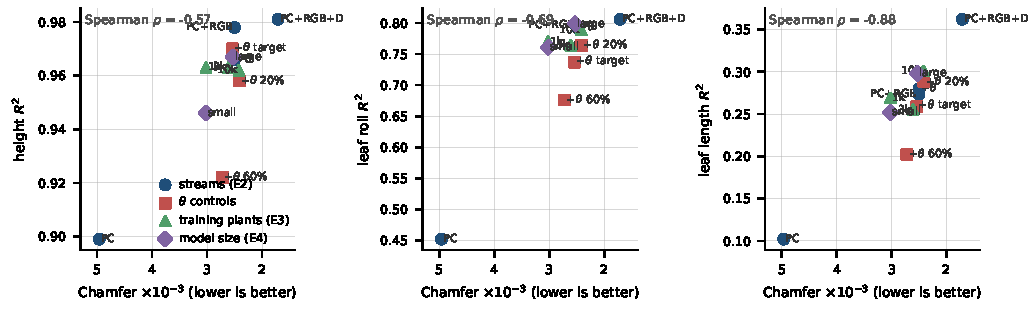
\includegraphics[width=\linewidth]{Figures/fig_metrics.pdf}
  \caption{\textbf{Divergence between Chamfer distance and frozen-latent trait probes.} Validation Chamfer distance plotted against height probe $R^2$ across twelve model variants.}
  \label{fig:metrics}\label{fig:metric_divergence}
\end{figure*}

\begin{figure}[t]
  \centering
  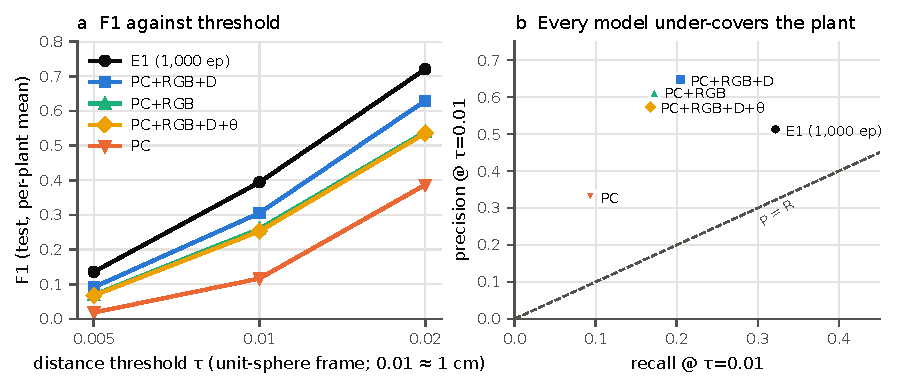
\includegraphics[width=\linewidth]{Figures/fig_fscore.pdf}
  \caption{\textbf{Point-cloud completion precision, recall, and $F_1$ score (sorghum test set).} \textbf{(a)} $F_1$ score across distance thresholds $\tau$. \textbf{(b)} Precision versus recall at $\tau = 0.01$. Precision consistently exceeds recall on thin plant foliage.}
  \label{fig:fscore}\label{fig:precision_recall}
\end{figure}
% REVIEWER FLAG: toned down as requested. "disagree on critical design choices" now reads "disagree on several design choices", and the loss ablation "confirms this mechanism" now reads "is consistent with this explanation".

\subsection{Representation Quality, Scaling, and Transfer}
\label{sec:res-repr}\label{sec:exp-repr}

\noindent\textbf{Comparison against published encoders.}
\tabref{tab:baselines} compares \method{} against DINOv2, MultiMAE, Point-MAE, and EmbodiedMAE, using identical mean-pooled token readouts and only the input modalities that each encoder supports (\appendixref{app:probe}). The three-stream \method{} ($\mathrm{PC}+\mathrm{RGB}+\mathrm{D}$) outperforms all baselines on 8 of 9 sorghum traits and 10 of 11 maize traits. Our 1{,}000-epoch headline model gives the strongest overall representation in the table, and it outperforms the published encoders on all eleven maize traits. Note that the full-pose Point-MAE appears artificially strong on synthetic maize due to a renderer artifact in which canonical leaf alignments leak the azimuth through the camera pose matrices. Under realistic gravity-aligned poses, the Point-MAE height $R^2$ drops from 0.720 to 0.588, whereas the pose-free \method{} is unaffected (\appendixref{app:probe}). Masked reconstruction comparisons are reported in \appendixref{sec:supp-recon}.

\begin{table*}[t]
  \caption{\textbf{Comparison against published self-supervised encoders.} We evaluate all encoders on the same held-out validation plants, using mean-pooled token features (excluding \texttt{[CLS]} for \method{}) and the same cross-validated ridge regression protocol. The encoders receive only the sensor modalities they were designed for. The values are validation $R^2$ (higher is better), and bold marks the best score in each column.}
  \label{tab:e8}\label{tab:baselines}
  \centering\scriptsize
  \setlength{\tabcolsep}{2.6pt}
  \begin{tabular}{l ccc cc c cccc}
    \toprule
    & \multicolumn{5}{c}{Sorghum} & & \multicolumn{4}{c}{Maize} \\
    \cmidrule(lr){2-6}\cmidrule(lr){8-11}
    Frozen Encoder & Height & Leaf Cnt & Branch & Roll & Leaf Len & & Height & Leaf Angle & Curl & Stem Rad \\
    \midrule
    DINOv2 ViT-B/14 (RGB)~\cite{oquab2024dinov2} & 0.924 & 0.928 & 0.840 & 0.573 & 0.235 & & 0.561 & 0.816 & 0.072 & 0.588 \\
    MultiMAE-B (RGB+D)~\cite{bachmann2022multimae} & 0.922 & 0.925 & 0.833 & 0.679 & 0.232 & & 0.570 & 0.783 & 0.069 & 0.442 \\
    Point-MAE (PC)~\cite{pang2022pointmae} & 0.958 & 0.963 & 0.863 & 0.716 & 0.188 & & 0.509 & 0.863 & 0.199 & 0.426 \\
    EmbodiedMAE-B (RGB+D+PC)~\cite{dong2025embodiedmae} & 0.976 & 0.979 & 0.871 & 0.765 & 0.265 & & 0.528 & 0.823 & 0.139 & 0.428 \\
    \CropCode{} Headline (1{,}000 ep) & \textbf{0.983} & \textbf{0.988} & \textbf{0.912} & \textbf{0.798} & \textbf{0.371} & & \textbf{0.747} & \textbf{0.967} & \textbf{0.739} & \textbf{0.841} \\
    \bottomrule
  \end{tabular}
\end{table*}
% REVIEWER FLAG: the Point-MAE maize height R^2 of 0.720 and 0.588 does not match Table tab:baselines, which lists 0.509 for Point-MAE (and the main body quotes "at most 0.570" for the published encoders). Numbers kept as in the source. Co-authors to state which probe protocol gives 0.720 and 0.588.
% REVIEWER FLAG: "8 of 9 sorghum traits and 10 of 11 maize traits" is stated here for the three-stream model against all baselines. Appendix app:probe states it against EmbodiedMAE-B only, and with the four-stream model for maize. Kept as in the source.

\noindent\textbf{Scaling, cross-species transfer, and latent geometry.}
\tabref{tab:scaling_ablations} and \figref{fig:data_model_scaling_fig} report the effect of the dataset size and the backbone capacity. Increasing the training dataset size from 1{,}000 to 10{,}500 plants reduces the Chamfer distance ($3.13 \to 2.53 \times 10^{-3}$ in sorghum and $3.54 \to 0.99 \times 10^{-3}$ in maize). The maize probe scores fluctuate at intermediate scales before peaking at the full dataset. Under a fixed gradient-step budget, scaling the backbone capacity from ViT-Base (114\,M) to ViT-Large (332\,M) degrades the representation quality in both species. Pretraining on maize and fine-tuning for 150 epochs on sorghum outperforms training from scratch on all probed traits (validation Chamfer $1.83$ vs.\ $3.38 \times 10^{-3}$), although the decoders do not transfer zero-shot across species. Finally, t-SNE projections of the frozen \texttt{[CLS]} tokens show smooth, continuous manifolds that are organized by plant scale and leaf posture, with no discrete clusters (\figref{fig:latent_tsne}). The effective participation ratios are low (4.4 to 6.3 of 768 dimensions in sorghum, and 6.7 to 11.3 in maize).

\begin{figure}[t]
  \centering
  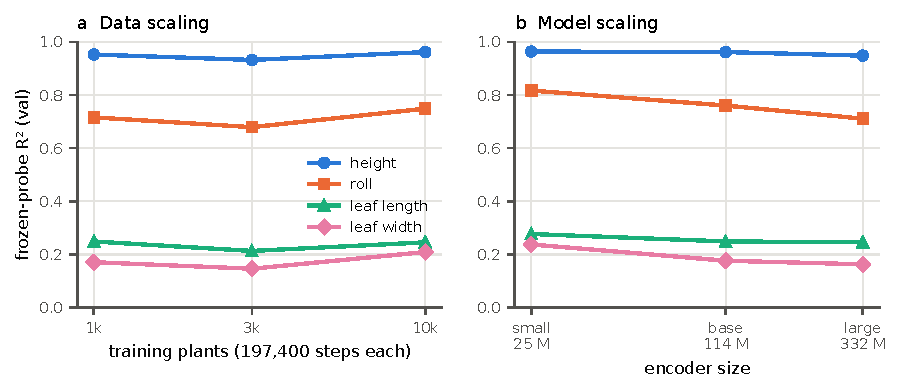
\includegraphics[width=\linewidth]{Figures/fig_scaling.pdf}
  \caption{\textbf{Dataset volume and model capacity scaling under equal gradient-step budgets (sorghum).} Validation linear-probe $R^2$ plotted against \textbf{(a)} training dataset size and \textbf{(b)} encoder parameter count.}
  \label{fig:data_model_scaling_fig}
\end{figure}

\begin{figure*}[!t]
  \centering
  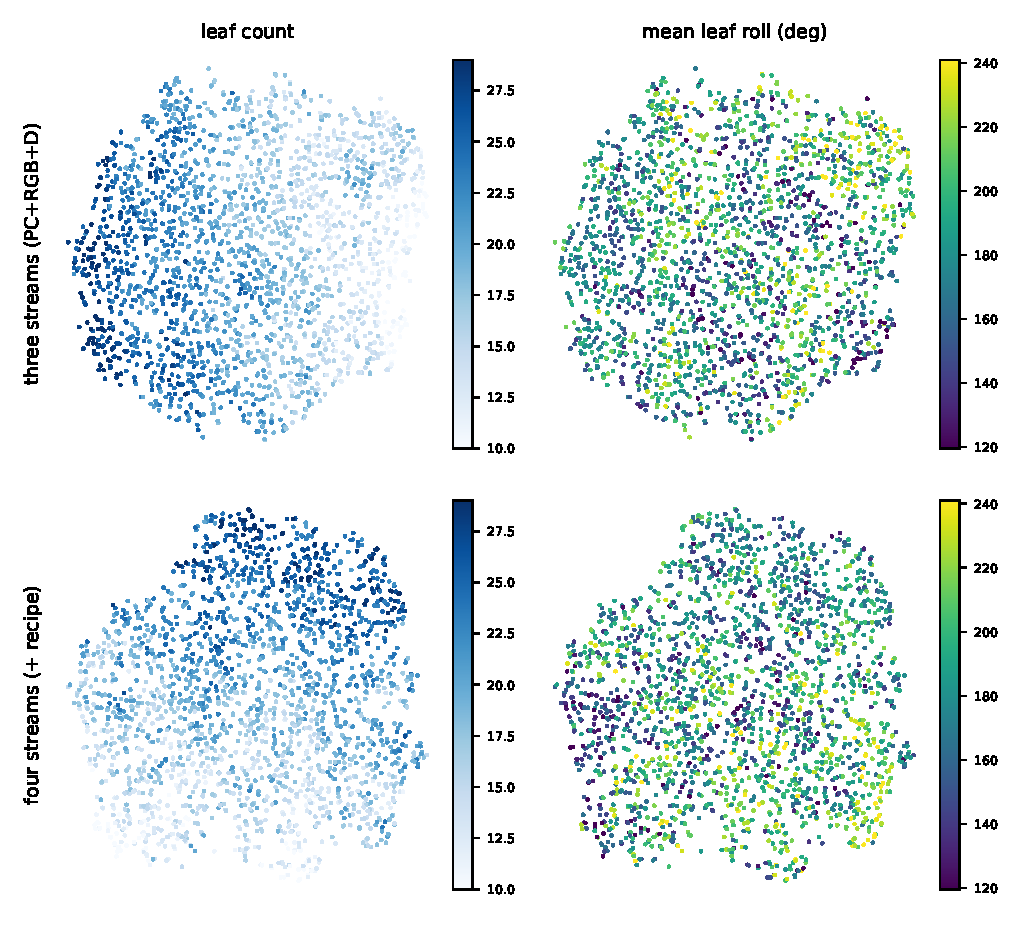
\includegraphics[width=0.85\linewidth]{Figures/fig_e9_tsne.pdf}
  \caption{\textbf{Latent space structure (sorghum validation set).} t-SNE embeddings of frozen \texttt{[CLS]} tokens for the 3-stream ($\mathrm{PC}+\mathrm{RGB}+\mathrm{D}$) and 4-stream ($+\theta$) models, colored by leaf count and mean leaf roll.}
  \label{fig:tsne}\label{fig:latent_tsne}
\end{figure*}





% \FloatBarrier   (removed 2026-11-23: it put Fig. S11 alone on a page)
% \clearpage   (removed 2026-11-23: it left blank space)
%%%%%%%%%%%%%%%%%%%%%%%%%%%%%%%%%%%%%%%%%%%%%%%%%%%%%%%%%%%%%%%%%%%%%%%%%%%
% APPENDIX C: IMPLEMENTATION AND EVALUATION DETAILS (moved verbatim from the main body of the earlier draft)
%%%%%%%%%%%%%%%%%%%%%%%%%%%%%%%%%%%%%%%%%%%%%%%%%%%%%%%%%%%%%%%%%%%%%%%%%%%
\section{Implementation and Evaluation Details}
\label{app:impl}

This appendix gives the full details of the tokenization, masking, training schedules, and evaluation protocols that are summarized in \textcolor{cvprblue}{Secs.}~\ref{sec:method-pretrain} and~\ref{sec:exp-setup}.

\noindent\textbf{Multimodal tokenization.}
We extend EmbodiedMAE~\citep{dong2025embodiedmae} and tokenize all four plant modalities into a unified sequence. RGB and depth images are partitioned into $14 \times 14 = 196$ patches and linearly projected to 768-dimensional embeddings with 2D sine-cosine positional encodings. Point clouds are grouped into 196 neighborhoods of 32 points via farthest-point sampling and encoded with a lightweight PointNet~\citep{pang2022pointmae,qi2017pointnet}. We structure the procedural parameter vector $\theta$ into $1 + K$ continuous numerical tokens, i.e., one global plant token followed by $K$ ordered leaf slots ($K = 28$ for maize, $K = 24$ for sorghum). These tokens are affinely normalized to $[0,1]$ and embedded using xVal-style continuous value scaling~\citep{golkar2023xval}. After adding learned modality embeddings and a global \texttt{[CLS]} token, the visible tokens are processed by a 12-block ViT encoder (width 768) and reconstructed by an 8-block decoder (width 512). The decoder has linear heads for RGB and depth, a FoldingNet head (41 points per token) for point clouds, and an MLP head for the procedural parameters. During training, the valid leaf slots are selected via a ground-truth existence mask. At test time without ground truth (\tabref{tab:regime1}, \appendixref{app:tables}), the leaf count is inferred directly from the predicted procedural parameters. It is stored explicitly in the plant token for maize, and it is derived from the predicted stem length for sorghum.

\noindent\textbf{Dynamic Dirichlet masking.}
To train a single network that can handle any subset of sensor inputs, we mask a fraction $\rho = 0.80$ of all tokens at each step. This leaves $V = \lfloor (1-\rho)L \rfloor$ visible tokens ($122$ of $L = 613$ tokens in sorghum, and $123$ of $617$ in maize). We allocate the visible tokens across the four streams using a symmetric Dirichlet draw at every iteration, constrained such that each active stream retains at least one visible token and at least 25\% masked tokens. In our default configuration, the parameter stream shares this visibility budget ($\sim 58\%$ visible on average). In the controlled ablations of \secref{sec:exp-params}, we instead gate the parameter visibility at a fixed rate $\rho_\theta$ (with $\rho_\theta = 1$ making the parameters a pure decoder reconstruction target).

\noindent\textbf{Training schedules.}
We train all models with AdamW and cosine learning-rate decay. Our headline models train for 1{,}000 epochs over all ten views (global batch size 256, peak learning rate $6 \times 10^{-4}$). The controlled ablations share a fixed compute budget of 197{,}400 steps (global batch size 32, one random view per plant per epoch, peak learning rate $1.5 \times 10^{-4}$) and use Eq.~\eqref{eq:qal}.

\noindent\textbf{Models and compute budgets.}
The controlled ablations use a ViT-Base backbone (114\,M parameters) trained for an identical budget of 197{,}400 optimizer steps at global batch size 32 (equivalent to 600 epochs of one random view per plant), with matched random view-sampling seeds. In the dataset-scaling experiments, we adjust the epoch counts to hold the total number of gradient steps constant. Our headline models train for 1{,}000 epochs across all ten views at global batch size 256 with the Sinkhorn objective (Eq.~\ref{eq:point-loss-sinkhorn}), and they initialize the teacher and student networks in \secref{sec:exp-main}. Unless noted otherwise, the ablation numbers are reported on the validation split.

\noindent\textbf{Field evaluation protocols.}
We evaluate \method{} with three complementary protocols:
\begin{enumerate}
  \item \textbf{Trait probing:} We fit ridge regression probes on the frozen \texttt{[CLS]} representations using the training split, and we evaluate $R^2$ on held-out plants. We use one deterministic view per plant, and we zero out the parameter inputs to prevent label leakage. A difference is counted as significant only when its 95\% paired-bootstrap confidence interval (2{,}000 plant resamples) excludes zero on both the validation and test splits. Under partial point-cloud visibility, the probes are either refit per visibility level (\emph{matched}) or transferred directly from complete clouds (\emph{transferred}).
  \item \textbf{Row occlusion:} We test both the zero-shot transfer of models trained only on isolated plants and the row fine-tuned models on simulated crop rows. The reconstruction accuracy is evaluated against the occluded target plant only, and we verify via an echo test that the models do not merely copy the neighboring foliage.
  \item \textbf{Real-plant validation:} We evaluate the row models on crop rows assembled from real MaizeField3D plants~\citep{maizefield3d2025}, and we use the procedural models released with that dataset as the ground truth.
% REVIEWER FLAG: the ground truth for the 520 real maize plants is now cited to the public MaizeField3D release only (confirmed by the author on 2026-11-14). The earlier text also cited the unpublished pipeline manuscript here, which is an anonymity risk.
\end{enumerate}
% REVIEWER FLAG: the Point-MAE maize height values here (0.720 and 0.588) do not match Table tab:baselines, which lists 0.509 for Point-MAE maize height. Numbers kept. Co-authors to state which protocol each value comes from.


%%%%%%%%%%%%%%%%%%%%%%%%%%%%%%%%%%%%%%%%%%%%%%%%%%%%%%%%%%%%%%%%%%%%%%%%%%%
% APPENDIX F: RESULT TABLES
%%%%%%%%%%%%%%%%%%%%%%%%%%%%%%%%%%%%%%%%%%%%%%%%%%%%%%%%%%%%%%%%%%%%%%%%%%%
\section{Result Tables}
\label{app:tables}

This appendix provides the full numerical tables referenced in the main paper, in the order of the main paper's experiments. We report simulated row occlusion (\tabref{tab:rows}; plotted in \figref{fig:rows}), the real-plant row experiments (\tabref{tab:e10} of the main paper and \tabref{tab:e10_detail}), \updtwo{the field rows of \secref{sec:supp-real-rows} (\tabref{tab:field_rows} and \tabref{tab:field_rows_single}),} and single-view reconstruction of isolated plants (\tabref{tab:regime1}). The remaining full tables appear beside their analyses: partial camera coverage (\tabref{tab:views}), the controlled modality, scale, and capacity ablations (\tabref{tab:modality_value_add}), the token-budget control ablations (\tabref{tab:control}), and the encoder comparison (\tabref{tab:baselines}) in \appendixref{app:analyses}, and any-subset cross-modal generation and distillation (\tabref{tab:anysubset}) in \appendixref{app:discussion}.
% REVIEWER FLAG (supplement reorder): this listing sentence was rewritten so the tables are named in the main paper's order (rows, real plants, single-sensor); the submitted version listed them as regime1 / views / rows / anysubset / control. No numbers changed.


\begin{table*}[t]
    \caption{\textbf{Single-view reconstruction on isolated plants.} Evaluation of the distilled generalist on fixed view 00 (unlike \tabref{tab:main}, which averages over random views) across 2{,}250 validation plants per species. $^{\dagger}$The undistilled headline model takes all three modalities under its 80\% masked pretraining regime (100\% visible tokens causes point cloud collapse). Leaf count and height are decoded directly from the predicted procedural parameters: maize stores leaf count explicitly, whereas sorghum derives it from predicted stem length ($\text{stem length} = 0.05n - 0.001$). Leaf-parameter skill is Eq.~\eqref{eq:trait-skill} averaged over active leaf slots; Chamfer distance ($\times 10^{-3}$) and $F_1$ are computed against the complete unit-sphere cloud, and RMS error converts unit-sphere Chamfer distance to millimeters (median scale: 1.03\,m sorghum, 0.61\,m maize). The three-view row averages predicted procedural parameters across views 00, 01, and 02. The two-stage baseline generates a point cloud from view 00 RGB before predicting procedural parameters from it, losing nearly all parameter accuracy (sorghum leaf skill drops from 0.656 to $-0.010$); this indicates that the procedural parameters should be predicted directly from the sensor data.}
  \label{tab:regime1}
  % REVIEWER FLAG: "confirming the advantage of direct end-to-end parameter inference" softened to "This indicates that the recipe should be predicted directly from the sensor data", matching the main body.
  % REVIEWER FLAG: the caption calls the gap to Table tab:main "slight", but the sorghum RGB Chamfer is 1.36 here vs. 0.88 there (depth 0.93 vs. 0.63). Wording kept. Co-authors to check.
  \centering\scriptsize
  \setlength{\tabcolsep}{4.5pt}
  \resizebox{\textwidth}{!}{%
\begin{tabular}{l cc c ccc}
    \toprule
    & Leaf Count & Height Error & Leaf Parameters & $F_1$-score & Chamfer & RMS Error \\
    Input Modality & (Acc. $\pm 1$) $\uparrow$ & (Rel. Err.) $\downarrow$ & (Mean Skill) $\uparrow$ & ($\tau=0.01$) $\uparrow$ & $\times10^{-3}\downarrow$ & (mm) $\downarrow$ \\
    \midrule
    \multicolumn{7}{l}{\emph{Sorghum}} \\
    RGB & 0.909 & 0.036 & 0.656 & 0.386 & 1.36 & 37.1 \\
    Depth & 0.956 & 0.026 & 0.679 & \textbf{0.440} & \textbf{0.93} & \textbf{30.3} \\
    Point Cloud & \textbf{0.998} & 0.022 & 0.675 & 0.370 & 1.45 & 38.7 \\
    $\mathrm{RGB}+\mathrm{D}+\mathrm{PC}$ (headline)$^\dagger$ & 0.889 & 0.038 & 0.636 & 0.392 & 1.36 & 37.0 \\
    RGB, three views (parameters averaged) & 0.995 & \textbf{0.018} & \textbf{0.747} & n/a& n/a& n/a\\
    \midrule
    Two-stage: RGB $\to$ point cloud $\to$ procedural parameters & 0.301 & 0.221 & $-0.010$ & 0.386 & 1.36 & 37.1 \\
    \midrule
    \multicolumn{7}{l}{\emph{Maize}} \\
    RGB & 0.973 & 0.045 & 0.567 & 0.482 & 0.83 & 13.6 \\
    Depth & 0.972 & 0.046 & 0.571 & \textbf{0.529} & \textbf{0.64} & \textbf{12.4} \\
    Point Cloud & 0.986 & \textbf{0.043} & 0.587 & 0.455 & 0.87 & 15.0 \\
    $\mathrm{RGB}+\mathrm{D}+\mathrm{PC}$ (headline)$^\dagger$ & 0.953 & 0.045 & 0.552 & 0.445 & 0.93 & 15.4 \\
    RGB, three views (parameters averaged) & \textbf{0.988} & 0.044 & \textbf{0.597} & n/a& n/a& n/a\\
    \midrule
    Two-stage: RGB $\to$ point cloud $\to$ procedural parameters & 0.066 & 0.131 & 0.015 & 0.482 & 0.83 & 13.6 \\
    \bottomrule
  \end{tabular}}
\end{table*}

\begin{table*}[t]
  \caption{\textbf{Reconstruction of identical plants in isolation versus simulated crop rows.} We evaluate 2{,}250 held-out test plants per species over 10 row orientations ($N = 22{,}500$). Chamfer distance is reported in metric units ($10^{-4}~\mathrm{m}^2$). $\Delta$ is the paired within-plant difference (row minus isolated), with 95\% bootstrap confidence intervals over plants.}
  \label{tab:rows}\label{tab:regime_3}
  % REVIEWER FLAG: bold is not defined in the caption and is not the column best. In the sorghum row fine-tuned block, 30.7 and 0.061 (all streams) are bold although depth-only is lower (18.6, 0.055). In maize, 0.046 is bold although the isolated control reaches 0.043. Table left unchanged.
  \centering\scriptsize
  \setlength{\tabcolsep}{3.0pt}
  \begin{tabular}{l l ccc ccc}
    \toprule
    & & \multicolumn{3}{c}{Chamfer vs.\ Target ($10^{-4}\,\mathrm{m}^2$)} & \multicolumn{3}{c}{Leaf Parameter MAE} \\
    \cmidrule(lr){3-5}\cmidrule(lr){6-8}
    Model Variant & Sensor Input & Isolated & Row & $\Delta$ [95\% CI] & Isolated & Row & $\Delta$ [95\% CI] \\
    \midrule
    \multicolumn{8}{l}{\emph{Maize: Zero-Shot (Headline Model)}} \\
    & RGB & 56.7 & 59.7 & $+3.0$\,{\scriptsize[$+2.4$, $+3.6$]} & 0.085 & 0.088 & $+0.003$\,{\scriptsize[$+0.003$, $+0.003$]} \\
    & Depth & 47.2 & 62.6 & $+15.3$\,{\scriptsize[$+14.8$, $+15.9$]} & 0.090 & 0.093 & $+0.002$\,{\scriptsize[$+0.002$, $+0.003$]} \\
    & Point Cloud & 20.0 & 33.8 & $+13.7$\,{\scriptsize[$+13.4$, $+14.1$]} & 0.064 & 0.081 & $+0.018$\,{\scriptsize[$+0.017$, $+0.018$]} \\
    & $\mathrm{RGB}+\mathrm{D}+\mathrm{PC}$ & 26.4 & 29.6 & $+3.2$\,{\scriptsize[$+2.9$, $+3.6$]} & 0.086 & 0.093 & $+0.007$\,{\scriptsize[$+0.007$, $+0.008$]} \\
    \midrule
    \multicolumn{8}{l}{\emph{Maize: Row Fine-Tuned}} \\
    & RGB & 13.7 & 14.4 & $+0.6$\,{\scriptsize[$+0.4$, $+0.8$]} & 0.067 & 0.071 & $+0.004$\,{\scriptsize[$+0.003$, $+0.004$]} \\
    & Depth & 10.3 & 9.6 & $-0.7$\,{\scriptsize[$-0.9$, $-0.5$]} & 0.061 & 0.064 & $+0.003$\,{\scriptsize[$+0.003$, $+0.004$]} \\
    & Point Cloud & 21.7 & 21.9 & $+0.2$\,{\scriptsize[$-0.1$, $+0.5$]} & 0.063 & 0.073 & $+0.010$\,{\scriptsize[$+0.010$, $+0.010$]} \\
    & $\mathrm{RGB}+\mathrm{D}+\mathrm{PC}$ & 12.6 & \textbf{4.0} & $-8.6$\,{\scriptsize[$-8.8$, $-8.3$]} & \textbf{0.046} & \textbf{0.052} & $+0.005$\,{\scriptsize[$+0.005$, $+0.005$]} \\
    \midrule
    \multicolumn{8}{l}{\emph{Maize: Isolated Control}} \\
    & RGB & 11.6 & 56.1 & $+44.5$\,{\scriptsize[$+44.0$, $+45.1$]} & 0.071 & 0.095 & $+0.024$\,{\scriptsize[$+0.023$, $+0.024$]} \\
    & Depth & 4.6 & 52.8 & $+48.2$\,{\scriptsize[$+47.5$, $+48.9$]} & 0.059 & 0.097 & $+0.038$\,{\scriptsize[$+0.037$, $+0.039$]} \\
    & Point Cloud & 8.2 & 25.1 & $+16.9$\,{\scriptsize[$+16.6$, $+17.3$]} & 0.046 & 0.076 & $+0.030$\,{\scriptsize[$+0.029$, $+0.030$]} \\
    & $\mathrm{RGB}+\mathrm{D}+\mathrm{PC}$ & 1.8 & 29.0 & $+27.2$\,{\scriptsize[$+26.9$, $+27.6$]} & 0.043 & 0.093 & $+0.050$\,{\scriptsize[$+0.049$, $+0.051$]} \\
    \midrule
    \multicolumn{8}{l}{\emph{Sorghum: Zero-Shot (Headline Model)}} \\
    & RGB & 163.1 & 218.5 & $+55.4$\,{\scriptsize[$+52.6$, $+58.4$]} & 0.129 & 0.135 & $+0.006$\,{\scriptsize[$+0.006$, $+0.006$]} \\
    & Depth & 106.2 & 207.2 & $+101.0$\,{\scriptsize[$+98.0$, $+104.2$]} & 0.070 & 0.109 & $+0.039$\,{\scriptsize[$+0.039$, $+0.040$]} \\
    & Point Cloud & 177.7 & 231.4 & $+53.8$\,{\scriptsize[$+52.2$, $+55.4$]} & 0.114 & 0.127 & $+0.013$\,{\scriptsize[$+0.012$, $+0.013$]} \\
    & $\mathrm{RGB}+\mathrm{D}+\mathrm{PC}$ & 174.3 & 230.5 & $+56.2$\,{\scriptsize[$+53.9$, $+58.5$]} & 0.108 & 0.114 & $+0.006$\,{\scriptsize[$+0.006$, $+0.006$]} \\
    \midrule
    \multicolumn{8}{l}{\emph{Sorghum: Row Fine-Tuned}} \\
    & RGB & 34.8 & 29.8 & $-5.0$\,{\scriptsize[$-5.4$, $-4.7$]} & 0.094 & 0.097 & $+0.003$\,{\scriptsize[$+0.003$, $+0.004$]} \\
    & Depth & 24.4 & 18.6 & $-5.8$\,{\scriptsize[$-6.1$, $-5.5$]} & 0.078 & 0.055 & $-0.022$\,{\scriptsize[$-0.023$, $-0.022$]} \\
    & Point Cloud & 46.0 & 70.8 & $+24.8$\,{\scriptsize[$+24.4$, $+25.2$]} & 0.074 & 0.082 & $+0.007$\,{\scriptsize[$+0.007$, $+0.007$]} \\
    & $\mathrm{RGB}+\mathrm{D}+\mathrm{PC}$ & 38.7 & \textbf{30.7} & $-8.0$\,{\scriptsize[$-8.5$, $-7.6$]} & \textbf{0.073} & \textbf{0.061} & $-0.012$\,{\scriptsize[$-0.013$, $-0.011$]} \\
    \midrule
    \multicolumn{8}{l}{\emph{Sorghum: Isolated Control}} \\
    & RGB & 15.7 & 133.2 & $+117.5$\,{\scriptsize[$+115.8$, $+119.3$]} & 0.094 & 0.114 & $+0.020$\,{\scriptsize[$+0.020$, $+0.021$]} \\
    & Depth & 6.6 & 171.9 & $+165.3$\,{\scriptsize[$+162.9$, $+167.8$]} & 0.042 & 0.100 & $+0.059$\,{\scriptsize[$+0.058$, $+0.060$]} \\
    & Point Cloud & 30.9 & 100.9 & $+70.0$\,{\scriptsize[$+68.8$, $+71.3$]} & 0.065 & 0.083 & $+0.018$\,{\scriptsize[$+0.018$, $+0.019$]} \\
    & $\mathrm{RGB}+\mathrm{D}+\mathrm{PC}$ & 13.1 & 133.8 & $+120.8$\,{\scriptsize[$+119.5$, $+122.1$]} & 0.049 & 0.096 & $+0.047$\,{\scriptsize[$+0.046$, $+0.048$]} \\
    \bottomrule
  \end{tabular}
\end{table*}


\begin{table*}[t]
  \caption{\textbf{Breakdown of real-row fine-tuning performance (held-out plants).} \textbf{Top:} Target Chamfer distance ($10^{-4}$\,m$^2$) for single-sensor and multi-sensor inputs, before (Row FT) and after (Real-row FT) fine-tuning on 75\% of the real plants. \textbf{Bottom:} Maize results (all three streams) stratified by ground-truth plant height. We show the median relative height error and the Chamfer distance. Note that the normalized height ceiling of the procedural parameter is 2.0\,m.}
  \label{tab:e10_detail}
  \centering\scriptsize
  \setlength{\tabcolsep}{3pt}
  {%
  \begin{tabular}{l cc cc}
    \toprule
    & \multicolumn{2}{c}{Maize (130 plants)} & \multicolumn{2}{c}{Sorghum (8 plants)} \\
    \cmidrule(lr){2-3}\cmidrule(lr){4-5}
    Input & Row FT & Real-row FT & Row FT & Real-row FT \\
    \midrule
    Image + depth + cloud & 59.5 & \textbf{19.7} & 2{,}113 & \textbf{79.4} \\
    Image only & 95.4 & 48.7 & 1{,}033 & 106.2 \\
    Depth only & 76.8 & 43.6 & 834 & 89.0 \\
    Cloud only & 75.0 & 47.4 & 3{,}773 & 311.8 \\
    \bottomrule
  \end{tabular}}

  \vspace{4pt}
  {%
  \begin{tabular}{l c cc cc}
    \toprule
    & & \multicolumn{2}{c}{Height error} & \multicolumn{2}{c}{Chamfer} \\
    \cmidrule(lr){3-4}\cmidrule(lr){5-6}
    Maize plant height & Plants & Row FT & Real-row FT & Row FT & Real-row FT \\
    \midrule
    $\le$1.33\,m (training range) & 22 & 15\% & \textbf{2.0\%} & 47.0 & \textbf{16.3} \\
    1.33 to 1.6\,m & 45 & 30\% & \textbf{1.2\%} & 57.7 & \textbf{18.8} \\
    1.6 to 2.0\,m & 51 & 41\% & \textbf{1.4\%} & 62.7 & \textbf{20.4} \\
    $>$2.0\,m & 12 & 51\% & \textbf{5.9\%} & 75.4 & \textbf{26.7} \\
    \bottomrule
  \end{tabular}}
\end{table*}

\updtwo{\noindent\textbf{Field rows from real plants.}
\tabref{tab:field_rows} and \tabref{tab:field_rows_single} report the field rows of \secref{sec:supp-real-rows}. The
plants are split by plant (sorghum: by scan, with its replicas), 351 / 39 / 130 maize plants and 33 / 5 / 13 sorghum
scans for training, validation and test. A test plant is the middle plant at several camera stops (1{,}555 maize and
1{,}484 sorghum test stops), and every model receives the 224-pixel window around the middle plant. The \emph{field
fine-tuned} models start from the row fine-tuned model and are trained for 30 epochs on the training plants (learning
rate $2\times10^{-5}$, batch size 16, random crops of the window). They are supervised on the middle plant's point cloud
and depth map, its height, and per leaf on the measured length and width, with the leaf count, internode distance and
curvature for maize and the insertion height for sorghum. The sorghum procedural model has no leaf-count field: the
generator derives the count from the stem length (0.05\,m per leaf), which does not hold for the real plants. Two further
sorghum runs therefore also train the leaf slots after the last real leaf to zero length and read the leaf count as the
number of slots longer than 5\,cm. The second of these also gives a single random input stream on half of the training
batches and weights the empty-slot term by 0.3.

Without fine-tuning, the models trained on synthetic data miss the real plants. The row fine-tuned model has a Chamfer
distance of 219 (maize) and 291 (sorghum) $\times10^{-4}$\,m$^2$ and a median height error of 37\% and 39\%. Field
fine-tuning reduces the Chamfer distance to 61 and 49, the height error to 4.0\% and 3.0\%, and the leaf length error
from 31 to 8.3\,cm in maize and from 27 to 10\,cm in sorghum, and it predicts the maize leaf count within one leaf at 69\%
of stops (53\% before). Training the empty leaf slots gives a sorghum leaf count within one leaf at 52\% of stops, at the
cost of 4\,cm in leaf length (10.2 to 14.4\,cm), but only with all three streams: from an image or a depth map alone the
count stays near the maximum of 24 leaves. Adding single-stream batches makes the count work from one sensor (image 50\%,
depth 40\%, point cloud 38\%), reduces the leaf length error to 12.3\,cm and the single-sensor Chamfer distance from 67 to
45, but lowers the count from all three streams to 40\%. In maize, whose field fine-tuning used all three streams only, a
single image or depth map still gives a median height error of about 50\%, against 9.4\% from the point cloud alone.}




%%%%%%%%%%%%%%%%%%%%%%%%%%%%%%%%%%%%%%%%%%%%%%%%%%%%%%%%%%%%%%%%%%%%%%%%%%%
% APPENDIX G: RESULT FIGURES
%%%%%%%%%%%%%%%%%%%%%%%%%%%%%%%%%%%%%%%%%%%%%%%%%%%%%%%%%%%%%%%%%%%%%%%%%%%
\section{Result Figures}
\label{app:figures}

We group the result figures below, in the order of the main paper's experiments: the quantitative row-occlusion results of \secref{sec:regime3} (\figref{fig:rows}), the real-plant rows of \secref{sec:exp-real} (\textcolor{cvprblue}{Figs.}~\ref{fig:e10_height}, \ref{fig:e10_real}, and~\ref{fig:e10_real_sorghum}), and the any-to-all cross-modal reconstructions of \secref{sec:exp-main} (\textcolor{cvprblue}{Figs.}~\ref{fig:any2any-maize} and~\ref{fig:any2any-sorghum}).
% (supplement reorder): the intro now names every figure in this section so each one is cited from the text.


% \begin{figure*}[t]
%   \centering
%   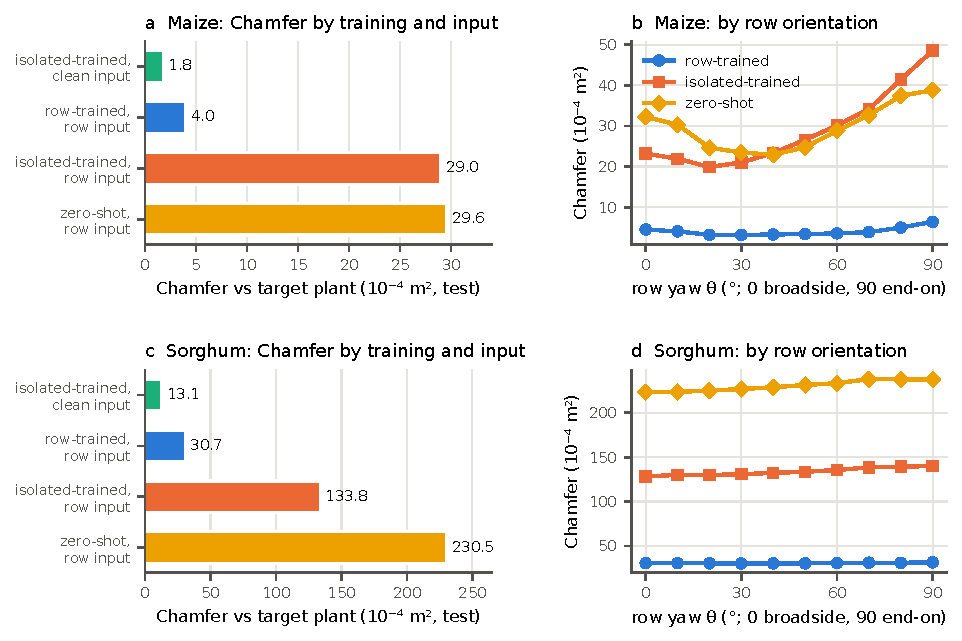
\includegraphics[width=\linewidth]{Figures/fig_rows.pdf}
%   \caption{\textbf{Quantitative row-occlusion performance on maize (a, b) and sorghum (c, d) test rows.} \textbf{(a, c)} Target plant Chamfer distance for the isolated control on isolated and row inputs, the row fine-tuned models on row inputs, and the zero-shot baselines. \textbf{(b, d)} Reconstruction error across row yaw angles ($\theta$). Row fine-tuning removes the vast majority of the neighbor-induced occlusion error in both species. In maize, whose leaves align roughly parallel to the row, the error peaks in broadside views, whereas the sorghum error does not depend on the row yaw.}
%   \label{fig:rows}\label{fig:row_reconstruction_quant}
% \end{figure*}

% \begin{figure}[t]
%   \centering
%   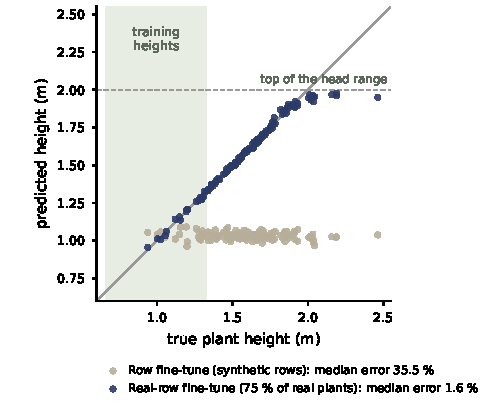
\includegraphics[width=0.99\linewidth]{Figures/fig_e10_height.pdf}
%   \caption{\textbf{Predicted versus true plant height on 130 held-out real maize plants} (median across the 36 camera stops of each plant, using all three input streams). When the model is trained only on synthetic rows, the predictions saturate near 1.03\,m. After fine-tuning on 75\% of the real plants, the predictions track the true height accurately up to the 2.0\,m recipe ceiling. The shaded region indicates the synthetic training height range.}
%   \label{fig:e10_height}
% \end{figure}

\begin{figure*}[t!]
  \centering
  % Top figure + standard bottom caption
  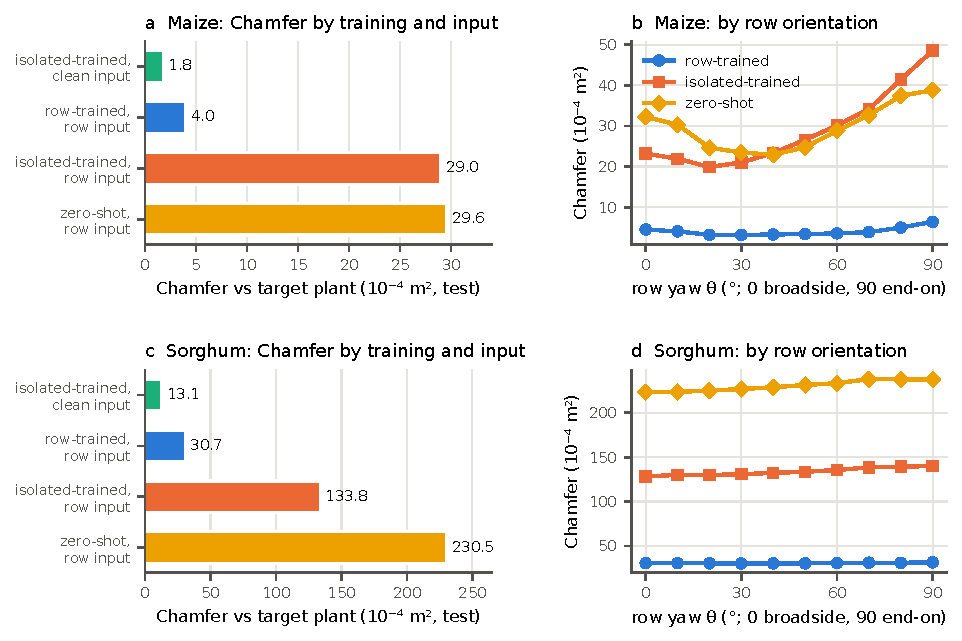
\includegraphics[width=0.88\textwidth]{Figures/fig_rows.pdf}
  \caption{\textbf{Quantitative row-occlusion performance on maize (a, b) and sorghum (c, d) test rows.} \textbf{(a, c)} Target plant Chamfer distance for the isolated control on isolated and row inputs, the row fine-tuned models on row inputs, and the zero-shot baselines. \textbf{(b, d)} Reconstruction error across row yaw angles ($\theta$). Row fine-tuning removes the vast majority of the neighbor-induced occlusion error in both species. In maize, whose leaves align roughly parallel to the row, the error peaks in broadside views, whereas the sorghum error does not depend on the row yaw.}
  \label{fig:rows}\label{fig:row_reconstruction_quant}

  \vspace{10pt}

  % Bottom figure centered + standard full-width bottom caption
  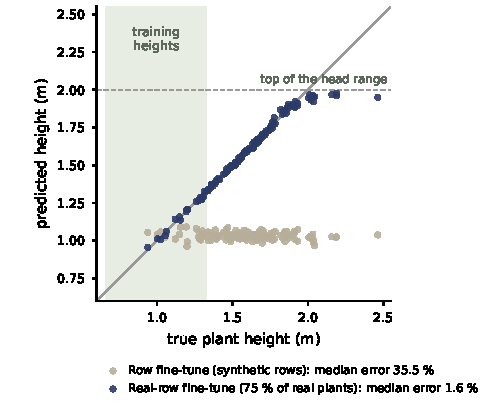
\includegraphics[width=0.48\textwidth]{Figures/fig_e10_height.pdf}
  \caption{\textbf{Predicted versus true plant height on 130 held-out real maize plants} (median across the 36 camera stops of each plant, using all three input streams). When the model is trained only on synthetic rows, the predictions saturate near 1.03\,m. After fine-tuning on 75\% of the real plants, the predictions track the true height accurately up to the 2.0\,m recipe ceiling. The shaded region indicates the synthetic training height range.}
  \label{fig:e10_height}
\end{figure*}

\begin{figure*}[t]
  \centering
  % 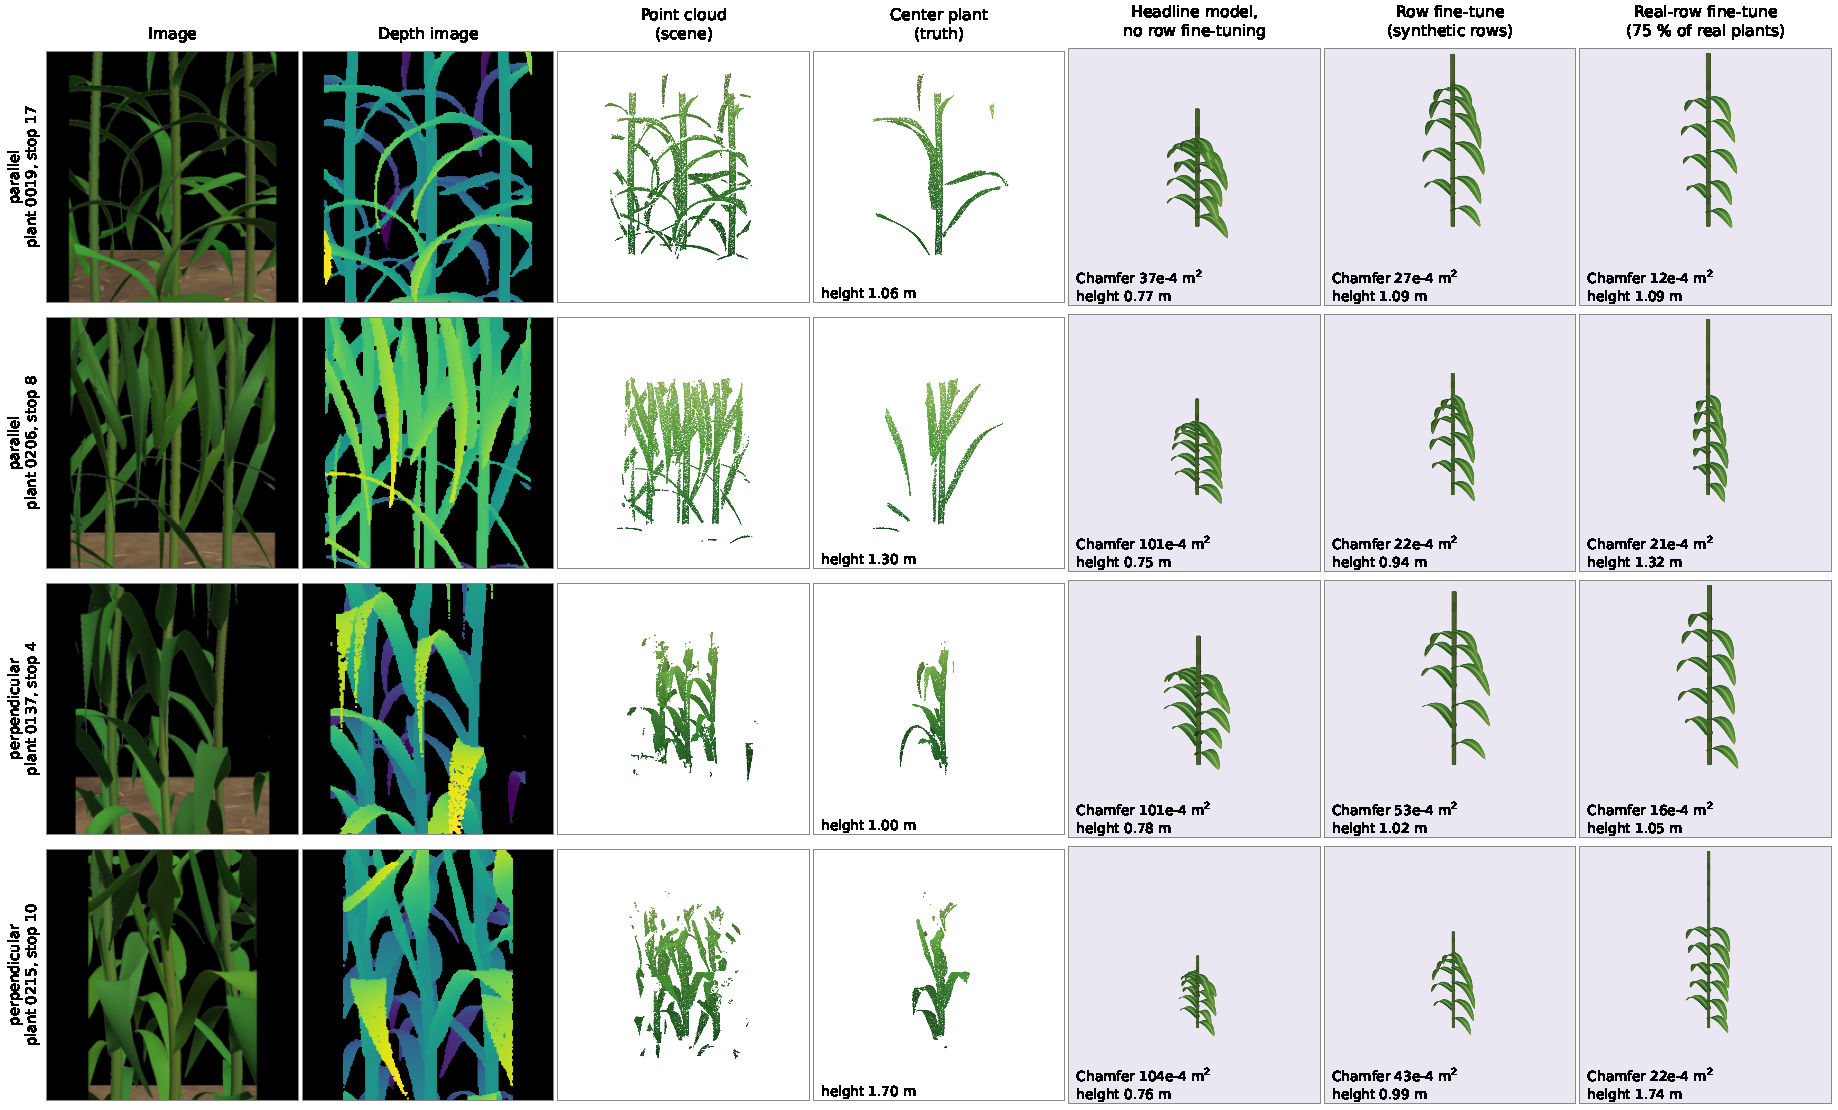
\includegraphics[width=\textwidth]{Figures/fig_e10_real_proc.pdf}
  \resizebox{\textwidth}{!}{% Generated by figures/_scene.py (Scene.render_tikz) for 'field rows maize'; do not edit by hand, re-run the figure script.
% 6.875 x 5.0738095238095235 in at 100 %; needs \usetikzlibrary{arrows.meta}; images in Figures/fig_e10_real/.
{%
\definecolor{c111111}{HTML}{111111}%
\definecolor{c1D221C}{HTML}{1D221C}%
\definecolor{c5E4A96}{HTML}{5E4A96}%
\definecolor{c6A2FD6}{HTML}{6A2FD6}%
\definecolor{c809EC2}{HTML}{809EC2}%
\definecolor{c9A9A9A}{HTML}{9A9A9A}%
\definecolor{c9D8CC4}{HTML}{9D8CC4}%
\definecolor{cD091A7}{HTML}{D091A7}%
\definecolor{cE0B020}{HTML}{E0B020}%
\definecolor{cE6ECF3}{HTML}{E6ECF3}%
\definecolor{cEAE7F2}{HTML}{EAE7F2}%
\definecolor{cF4F4F5}{HTML}{F4F4F5}%
\definecolor{cF6E9ED}{HTML}{F6E9ED}%
\definecolor{cFAF2D4}{HTML}{FAF2D4}%
\begin{tikzpicture}[x=1in, y=1in]%
\useasboundingbox (0,0) rectangle (6.8750,5.0738);
\draw[draw=c809EC2, line width=1.000pt, fill=cE6ECF3, dash pattern=on 3.00pt off 2.00pt, rounded corners=0.0300in] (0.7800,3.5929) rectangle (1.6207,4.7138);
\draw[draw=cE0B020, line width=1.000pt, fill=cFAF2D4, dash pattern=on 3.00pt off 2.00pt, rounded corners=0.0300in] (1.6557,3.5929) rectangle (2.4964,4.7138);
\draw[draw=cD091A7, line width=1.000pt, fill=cF6E9ED, dash pattern=on 3.00pt off 2.00pt, rounded corners=0.0300in] (2.5314,3.5929) rectangle (3.3721,4.7138);
\draw[draw=c9A9A9A, line width=1.000pt, fill=cF4F4F5, rounded corners=0.0300in] (3.4071,3.5929) rectangle (4.2479,4.7138);
\draw[draw=c9D8CC4, line width=1.000pt, fill=cEAE7F2, rounded corners=0.0300in] (4.2829,3.5929) rectangle (5.1236,4.7138);
\draw[draw=c9D8CC4, line width=1.000pt, fill=cEAE7F2, rounded corners=0.0300in] (5.1586,3.5929) rectangle (5.9993,4.7138);
\draw[draw=c9D8CC4, line width=1.000pt, fill=cEAE7F2, rounded corners=0.0300in] (6.0343,3.5929) rectangle (6.8750,4.7138);
\draw[draw=c809EC2, line width=1.000pt, fill=cE6ECF3, dash pattern=on 3.00pt off 2.00pt, rounded corners=0.0300in] (0.7800,2.4019) rectangle (1.6207,3.5229);
\draw[draw=cE0B020, line width=1.000pt, fill=cFAF2D4, dash pattern=on 3.00pt off 2.00pt, rounded corners=0.0300in] (1.6557,2.4019) rectangle (2.4964,3.5229);
\draw[draw=cD091A7, line width=1.000pt, fill=cF6E9ED, dash pattern=on 3.00pt off 2.00pt, rounded corners=0.0300in] (2.5314,2.4019) rectangle (3.3721,3.5229);
\draw[draw=c9A9A9A, line width=1.000pt, fill=cF4F4F5, rounded corners=0.0300in] (3.4071,2.4019) rectangle (4.2479,3.5229);
\draw[draw=c9D8CC4, line width=1.000pt, fill=cEAE7F2, rounded corners=0.0300in] (4.2829,2.4019) rectangle (5.1236,3.5229);
\draw[draw=c9D8CC4, line width=1.000pt, fill=cEAE7F2, rounded corners=0.0300in] (5.1586,2.4019) rectangle (5.9993,3.5229);
\draw[draw=c9D8CC4, line width=1.000pt, fill=cEAE7F2, rounded corners=0.0300in] (6.0343,2.4019) rectangle (6.8750,3.5229);
\draw[draw=c809EC2, line width=1.000pt, fill=cE6ECF3, dash pattern=on 3.00pt off 2.00pt, rounded corners=0.0300in] (0.7800,1.2110) rectangle (1.6207,2.3319);
\draw[draw=cE0B020, line width=1.000pt, fill=cFAF2D4, dash pattern=on 3.00pt off 2.00pt, rounded corners=0.0300in] (1.6557,1.2110) rectangle (2.4964,2.3319);
\draw[draw=cD091A7, line width=1.000pt, fill=cF6E9ED, dash pattern=on 3.00pt off 2.00pt, rounded corners=0.0300in] (2.5314,1.2110) rectangle (3.3721,2.3319);
\draw[draw=c9A9A9A, line width=1.000pt, fill=cF4F4F5, rounded corners=0.0300in] (3.4071,1.2110) rectangle (4.2479,2.3319);
\draw[draw=c9D8CC4, line width=1.000pt, fill=cEAE7F2, rounded corners=0.0300in] (4.2829,1.2110) rectangle (5.1236,2.3319);
\draw[draw=c9D8CC4, line width=1.000pt, fill=cEAE7F2, rounded corners=0.0300in] (5.1586,1.2110) rectangle (5.9993,2.3319);
\draw[draw=c9D8CC4, line width=1.000pt, fill=cEAE7F2, rounded corners=0.0300in] (6.0343,1.2110) rectangle (6.8750,2.3319);
\draw[draw=c809EC2, line width=1.000pt, fill=cE6ECF3, dash pattern=on 3.00pt off 2.00pt, rounded corners=0.0300in] (0.7800,0.0200) rectangle (1.6207,1.1410);
\draw[draw=cE0B020, line width=1.000pt, fill=cFAF2D4, dash pattern=on 3.00pt off 2.00pt, rounded corners=0.0300in] (1.6557,0.0200) rectangle (2.4964,1.1410);
\draw[draw=cD091A7, line width=1.000pt, fill=cF6E9ED, dash pattern=on 3.00pt off 2.00pt, rounded corners=0.0300in] (2.5314,0.0200) rectangle (3.3721,1.1410);
\draw[draw=c9A9A9A, line width=1.000pt, fill=cF4F4F5, rounded corners=0.0300in] (3.4071,0.0200) rectangle (4.2479,1.1410);
\draw[draw=c9D8CC4, line width=1.000pt, fill=cEAE7F2, rounded corners=0.0300in] (4.2829,0.0200) rectangle (5.1236,1.1410);
\draw[draw=c9D8CC4, line width=1.000pt, fill=cEAE7F2, rounded corners=0.0300in] (5.1586,0.0200) rectangle (5.9993,1.1410);
\draw[draw=c9D8CC4, line width=1.000pt, fill=cEAE7F2, rounded corners=0.0300in] (6.0343,0.0200) rectangle (6.8750,1.1410);
\node[anchor=south west, inner sep=0] at (0.8000,3.6129) {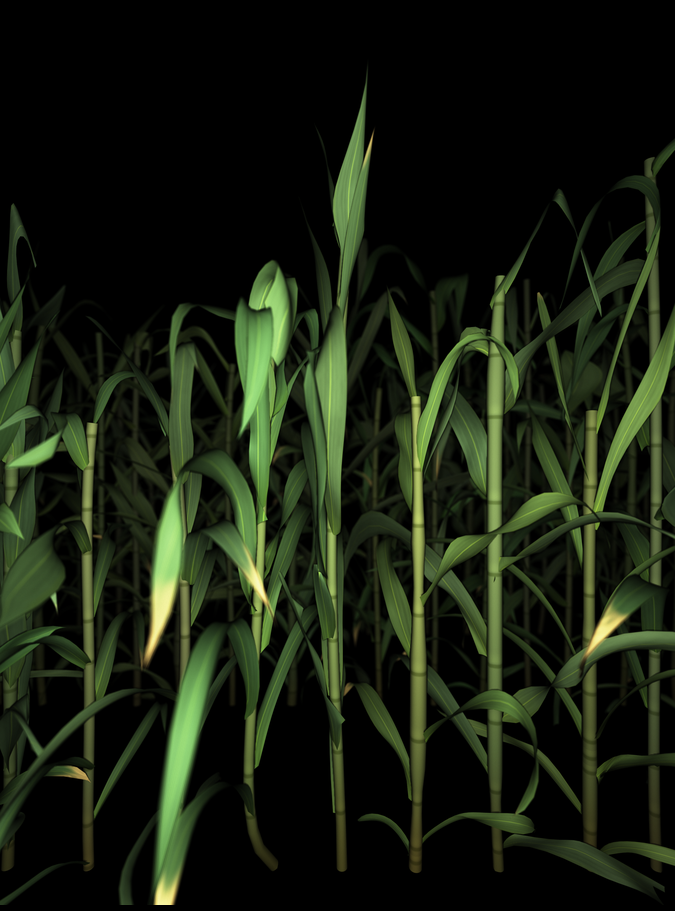
\includegraphics[width=0.8007in, height=1.0810in]{Figures/fig_e10_real/maize_0_image.png}};
\node[anchor=south west, inner sep=0] at (1.6757,3.6129) {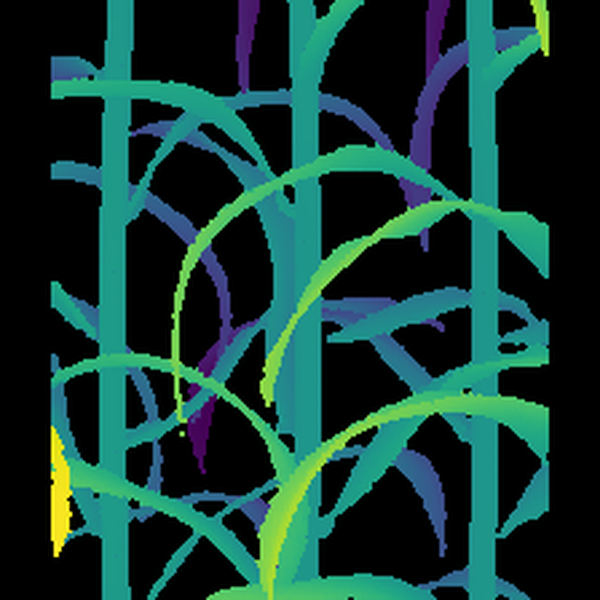
\includegraphics[width=0.8007in, height=1.0810in]{Figures/fig_e10_real/maize_0_depth.png}};
\node[anchor=south west, inner sep=0] at (2.5514,3.6129) {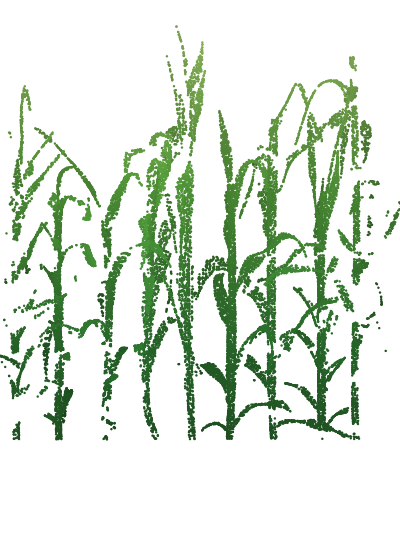
\includegraphics[width=0.8007in, height=1.0810in]{Figures/fig_e10_real/maize_0_cloud_2.png}};
\node[anchor=south west, inner sep=0] at (3.4271,3.9047) {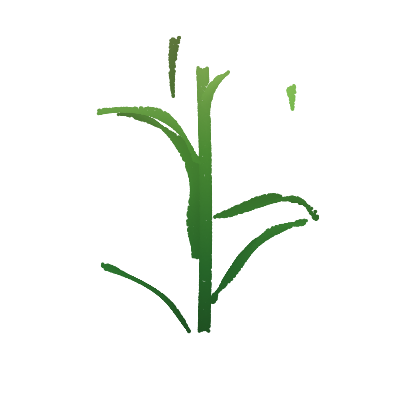
\includegraphics[width=0.8007in, height=0.7891in]{Figures/fig_e10_real/maize_0_cloud_3.png}};
\node[anchor=south west, inner sep=0] at (4.3029,3.9047) {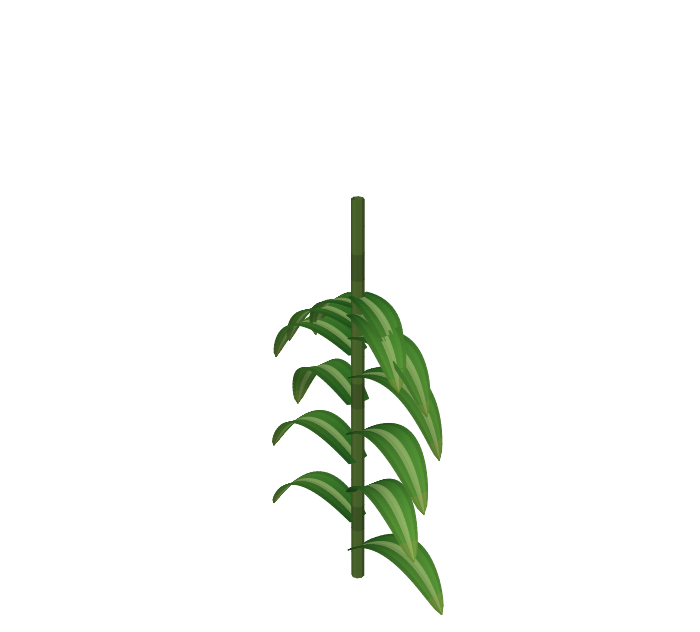
\includegraphics[width=0.8007in, height=0.7891in]{Figures/fig_e10_real/maize_0_pred_0.png}};
\node[anchor=south west, inner sep=0] at (5.1786,3.9047) {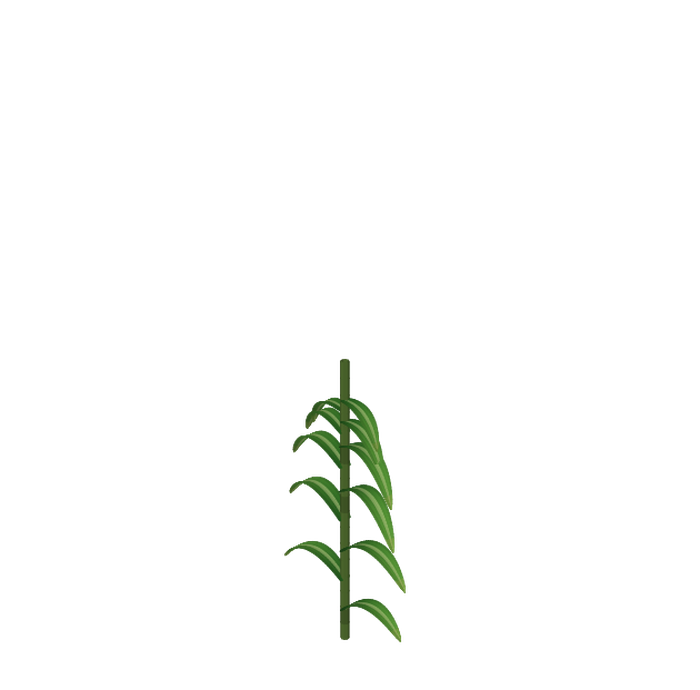
\includegraphics[width=0.8007in, height=0.7891in]{Figures/fig_e10_real/maize_0_pred_1.png}};
\node[anchor=south west, inner sep=0] at (6.0543,3.9047) {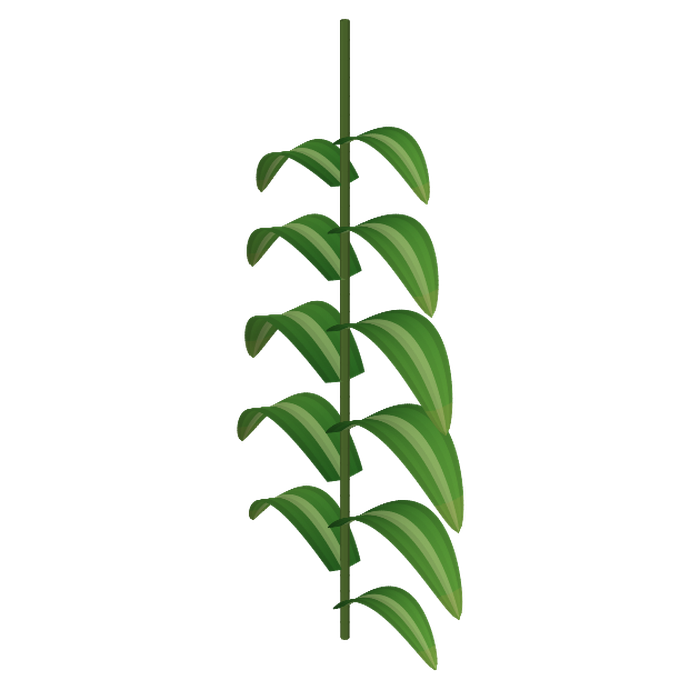
\includegraphics[width=0.8007in, height=0.7891in]{Figures/fig_e10_real/maize_0_pred_2.png}};
\node[anchor=south west, inner sep=0] at (0.8000,2.4219) {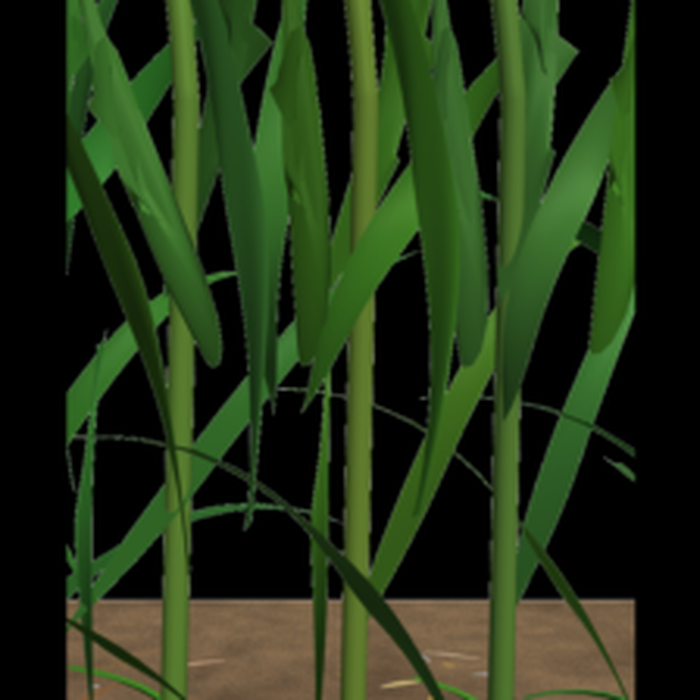
\includegraphics[width=0.8007in, height=1.0810in]{Figures/fig_e10_real/maize_1_image.png}};
\node[anchor=south west, inner sep=0] at (1.6757,2.4219) {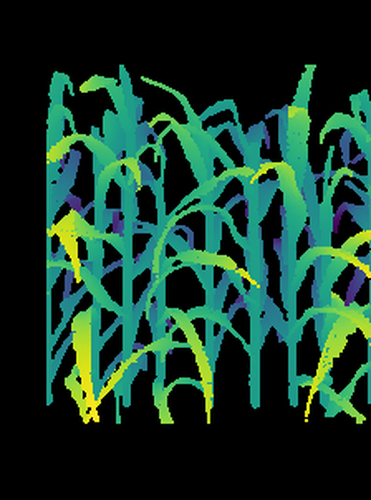
\includegraphics[width=0.8007in, height=1.0810in]{Figures/fig_e10_real/maize_1_depth.png}};
\node[anchor=south west, inner sep=0] at (2.5514,2.4219) {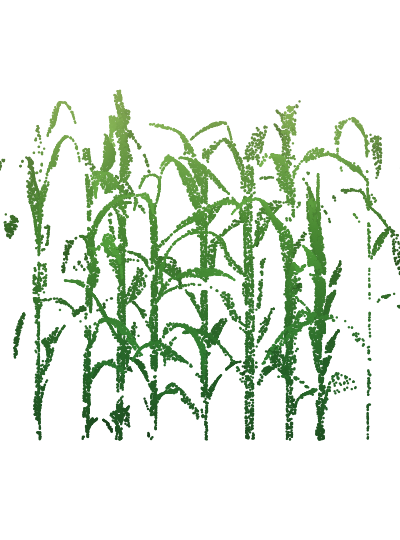
\includegraphics[width=0.8007in, height=1.0810in]{Figures/fig_e10_real/maize_1_cloud_2.png}};
\node[anchor=south west, inner sep=0] at (3.4271,2.7138) {
\includegraphics[width=0.8007in, height=0.7891in]{Figures/fig_e10_real/maize_1_cloud_3.png}};
\node[anchor=south west, inner sep=0] at (4.3029,2.7138) {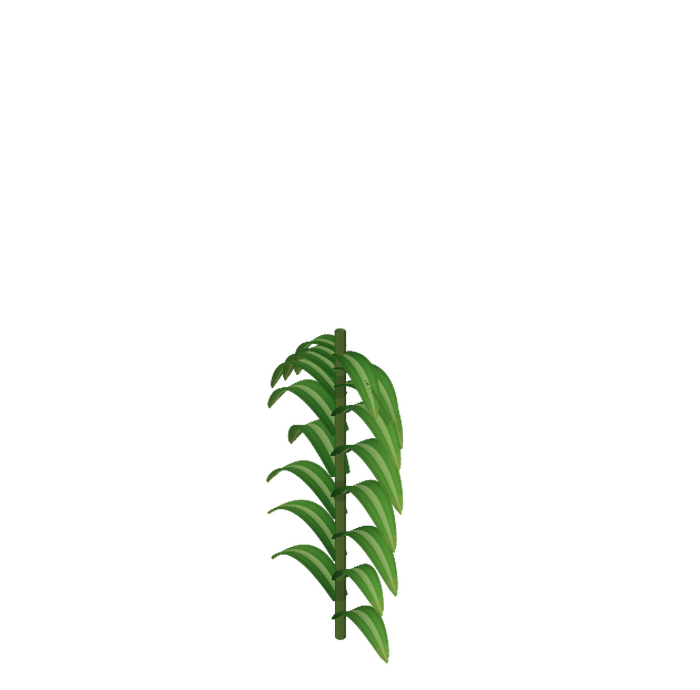
\includegraphics[width=0.8007in, height=0.7891in]{Figures/fig_e10_real/maize_1_pred_0.png}};
\node[anchor=south west, inner sep=0] at (5.1786,2.7138) {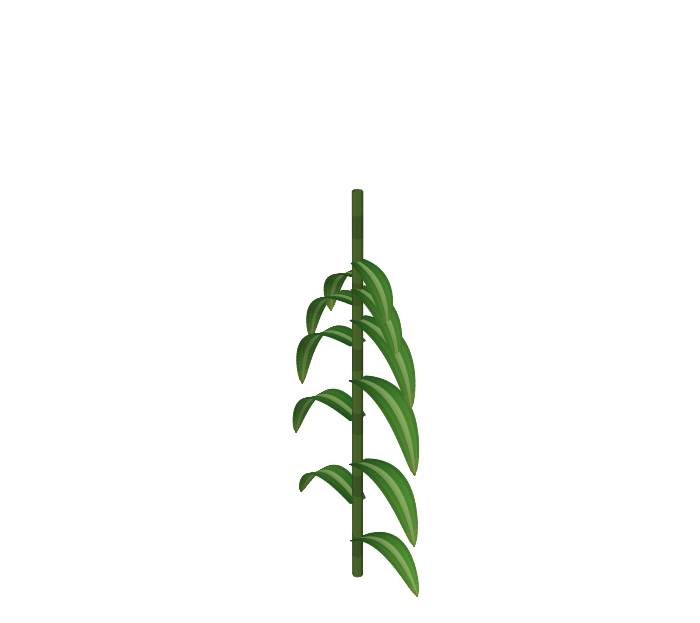
\includegraphics[width=0.8007in, height=0.7891in]{Figures/fig_e10_real/maize_1_pred_1.png}};
\node[anchor=south west, inner sep=0] at (6.0543,2.7138) {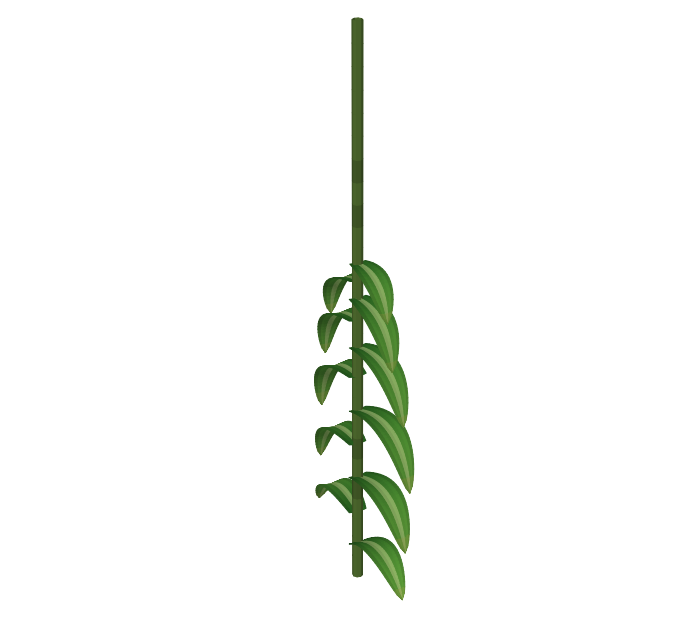
\includegraphics[width=0.8007in, height=0.7891in]{Figures/fig_e10_real/maize_1_pred_2.png}};
\node[anchor=south west, inner sep=0] at (0.8000,1.2310) {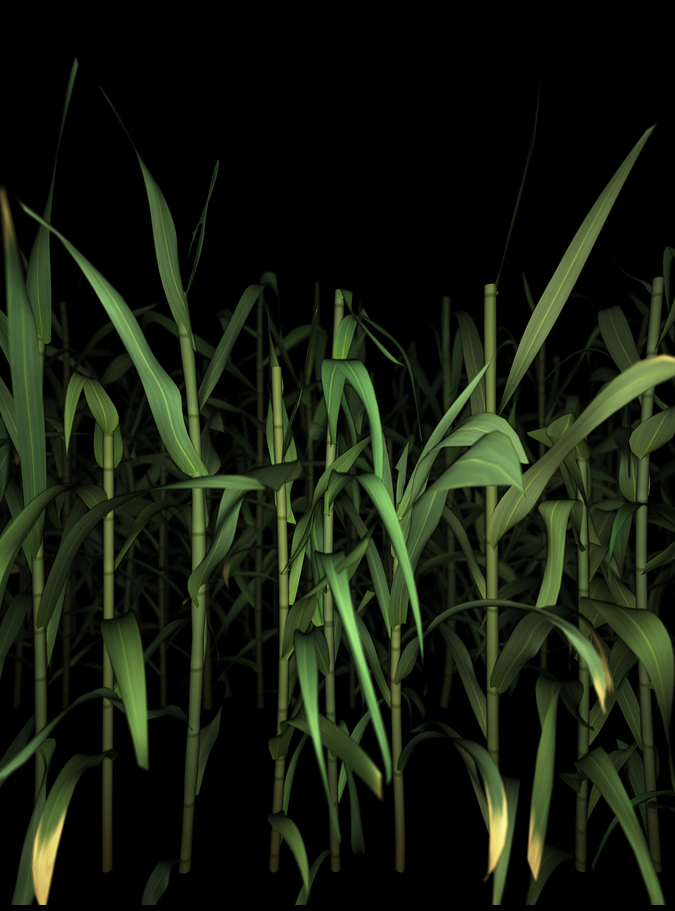
\includegraphics[width=0.8007in, height=1.0810in]{Figures/fig_e10_real/maize_2_image.png}};
\node[anchor=south west, inner sep=0] at (1.6757,1.2310) {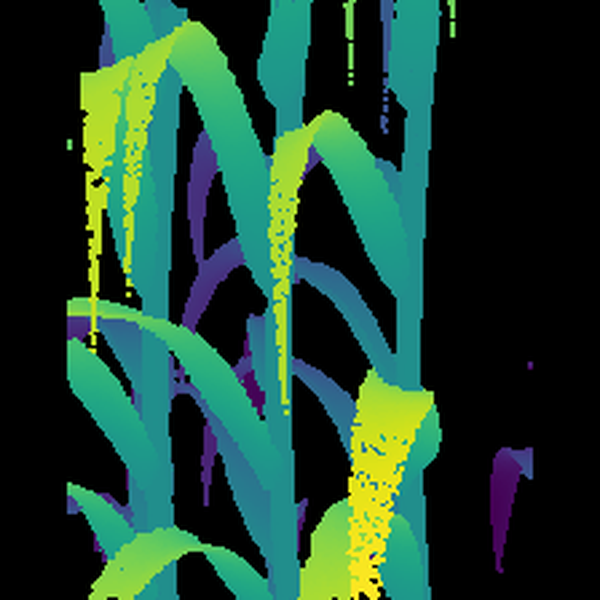
\includegraphics[width=0.8007in, height=1.0810in]{Figures/fig_e10_real/maize_2_depth.png}};
\node[anchor=south west, inner sep=0] at (2.5514,1.2310) {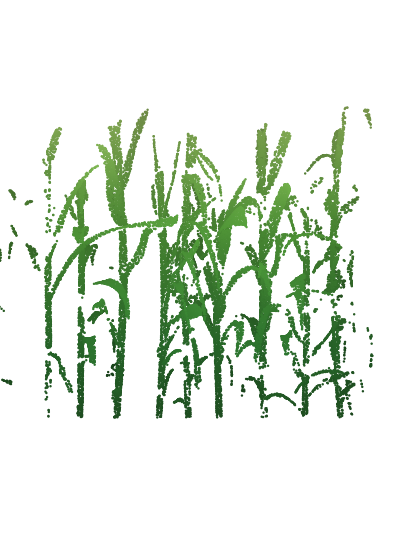
\includegraphics[width=0.8007in, height=1.0810in]{Figures/fig_e10_real/maize_2_cloud_2.png}};
\node[anchor=south west, inner sep=0] at (3.4271,1.5228) {
\includegraphics[width=0.8007in, height=0.7891in]{Figures/fig_e10_real/maize_2_cloud_3.png}};
\node[anchor=south west, inner sep=0] at (4.3029,1.5228) {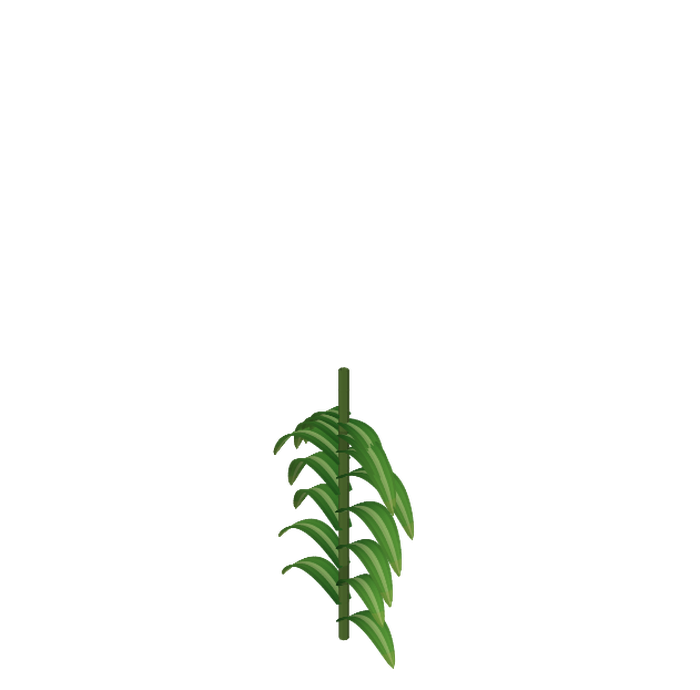
\includegraphics[width=0.8007in, height=0.7891in]{Figures/fig_e10_real/maize_2_pred_0.png}};
\node[anchor=south west, inner sep=0] at (5.1786,1.5228) {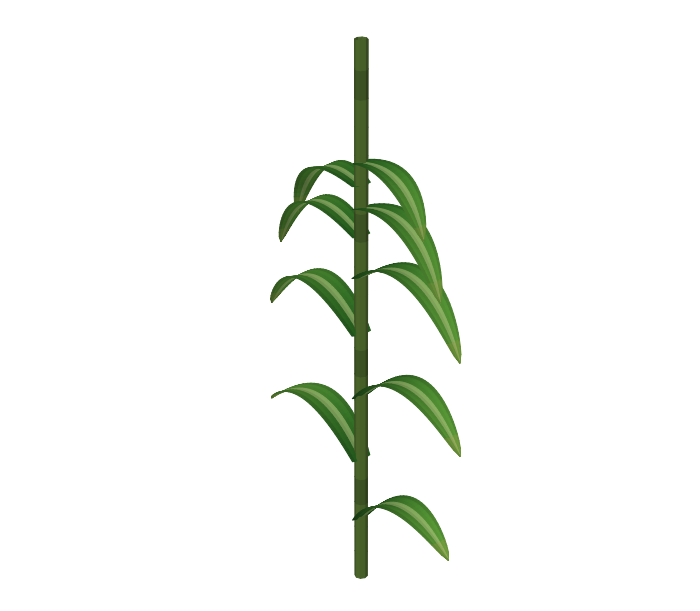
\includegraphics[width=0.8007in, height=0.7891in]{Figures/fig_e10_real/maize_2_pred_1.png}};
\node[anchor=south west, inner sep=0] at (6.0543,1.5228) {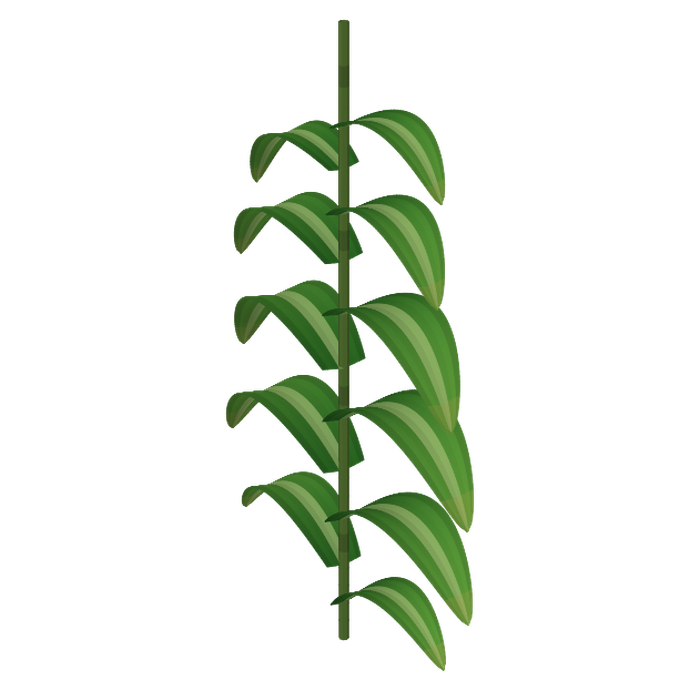
\includegraphics[width=0.8007in, height=0.7891in]{Figures/fig_e10_real/maize_2_pred_2.png}};
\node[anchor=south west, inner sep=0] at (0.8000,0.0400) {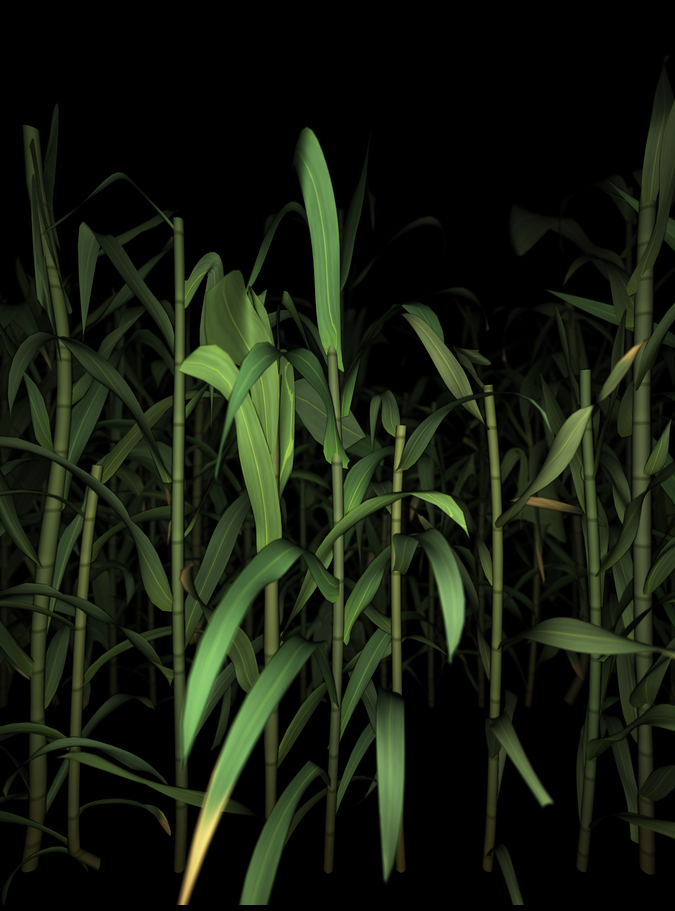
\includegraphics[width=0.8007in, height=1.0810in]{Figures/fig_e10_real/maize_3_image.png}};
\node[anchor=south west, inner sep=0] at (1.6757,0.0400) {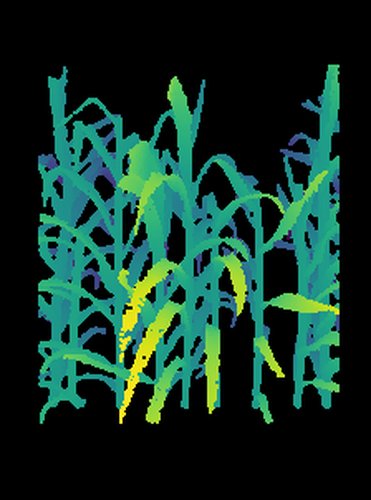
\includegraphics[width=0.8007in, height=1.0810in]{Figures/fig_e10_real/maize_3_depth.png}};
\node[anchor=south west, inner sep=0] at (2.5514,0.0400) {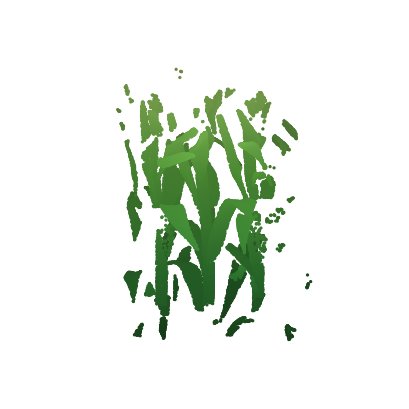
\includegraphics[width=0.8007in, height=1.0810in]{Figures/fig_e10_real/maize_3_cloud_2.png}};
\node[anchor=south west, inner sep=0] at (3.4271,0.3319) {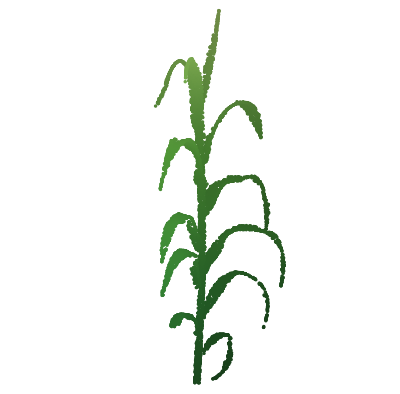
\includegraphics[width=0.8007in, height=0.7891in]{Figures/fig_e10_real/maize_3_cloud_3.png}};
\node[anchor=south west, inner sep=0] at (4.3029,0.3319) {\includegraphics[width=0.8007in, height=0.7891in]{Figures/fig_e10_real/maize_3_pred_0.png}};
\node[anchor=south west, inner sep=0] at (5.1786,0.3319) {\includegraphics[width=0.8007in, height=0.7891in]{Figures/fig_e10_real/maize_3_pred_1.png}};
\node[anchor=south west, inner sep=0] at (6.0543,0.3319) {\includegraphics[width=0.8007in, height=0.7891in]{Figures/fig_e10_real/maize_3_pred_2.png}};
\node[anchor=north, inner sep=0, outer sep=0, align=center, text=c111111, font={\fontsize{6.40}{6.72}\selectfont\sffamily}] at (1.2004,5.0638) {Image};
\node[anchor=north, inner sep=0, outer sep=0, align=center, text=c111111, font={\fontsize{6.40}{6.72}\selectfont\sffamily}] at (2.0761,5.0638) {Depth image};
\node[anchor=north, inner sep=0, outer sep=0, align=center, text=c111111, font={\fontsize{6.40}{6.72}\selectfont\sffamily}] at (2.9518,5.0638) {Point cloud\\(scene)};
\node[anchor=north, inner sep=0, outer sep=0, align=center, text=c111111, font={\fontsize{6.40}{6.72}\selectfont\sffamily}] at (3.8275,5.0638) {Center plant\\(truth)};
\node[anchor=north, inner sep=0, outer sep=0, align=center, text=c5E4A96, font={\fontsize{6.40}{6.72}\selectfont\sffamily}] at (4.7032,5.0638) {No row\\training};
\node[anchor=north, inner sep=0, outer sep=0, align=center, text=c5E4A96, font={\fontsize{6.40}{6.72}\selectfont\sffamily}] at (5.5789,5.0638) {Synthetic-row\\fine-tune};
\node[anchor=north, inner sep=0, outer sep=0, align=center, text=c6A2FD6, font={\fontsize{6.40}{6.72}\selectfont\sffamily}] at (6.4546,5.0638) {Field\\fine-tune};
\node[anchor=south west, inner sep=0, outer sep=0, align=left, text=c1D221C, font={\fontsize{5.80}{6.38}\selectfont\sffamily}] at (3.4672,3.6369) {1.91 m\\11 leaves};
\node[anchor=south west, inner sep=0, outer sep=0, align=left, text=c5E4A96, font={\fontsize{5.80}{6.38}\selectfont\sffamily}] at (4.3429,3.6369) {CD = 491\\0.72 m, 16 leaves};
\node[anchor=south west, inner sep=0, outer sep=0, align=left, text=c5E4A96, font={\fontsize{5.80}{6.38}\selectfont\sffamily}] at (5.2186,3.6369) {CD = 297\\0.87 m, 11 leaves};
\node[anchor=south west, inner sep=0, outer sep=0, align=left, text=c6A2FD6, font={\fontsize{5.80}{6.38}\selectfont\sffamily}] at (6.0943,3.6369) {CD = 62\\1.84 m, 11 leaves};
\node[anchor=east, inner sep=0, outer sep=0, align=right, text=c1D221C, font={\fontsize{6.20}{6.82}\selectfont\sffamily}] at (0.7000,4.1533) {plant\\0204\\row 936\\stop 6};
\node[anchor=south west, inner sep=0, outer sep=0, align=left, text=c1D221C, font={\fontsize{5.80}{6.38}\selectfont\sffamily}] at (3.4672,2.4459) {1.49 m\\10 leaves};
\node[anchor=south west, inner sep=0, outer sep=0, align=left, text=c5E4A96, font={\fontsize{5.80}{6.38}\selectfont\sffamily}] at (4.3429,2.4459) {CD = 143\\0.78 m, 18 leaves};
\node[anchor=south west, inner sep=0, outer sep=0, align=left, text=c5E4A96, font={\fontsize{5.80}{6.38}\selectfont\sffamily}] at (5.2186,2.4459) {CD = 103\\0.86 m, 10 leaves};
\node[anchor=south west, inner sep=0, outer sep=0, align=left, text=c6A2FD6, font={\fontsize{5.80}{6.38}\selectfont\sffamily}] at (6.0943,2.4459) {CD = 69\\1.48 m, 11 leaves};
\node[anchor=east, inner sep=0, outer sep=0, align=right, text=c1D221C, font={\fontsize{6.20}{6.82}\selectfont\sffamily}] at (0.7000,2.9624) {plant\\0064\\row 539\\stop 6};
\node[anchor=south west, inner sep=0, outer sep=0, align=left, text=c1D221C, font={\fontsize{5.80}{6.38}\selectfont\sffamily}] at (3.4672,1.2550) {1.51 m\\14 leaves};
\node[anchor=south west, inner sep=0, outer sep=0, align=left, text=c5E4A96, font={\fontsize{5.80}{6.38}\selectfont\sffamily}] at (4.3429,1.2550) {CD = 234\\0.74 m, 16 leaves};
\node[anchor=south west, inner sep=0, outer sep=0, align=left, text=c5E4A96, font={\fontsize{5.80}{6.38}\selectfont\sffamily}] at (5.2186,1.2550) {CD = 116\\0.90 m, 11 leaves};
\node[anchor=south west, inner sep=0, outer sep=0, align=left, text=c6A2FD6, font={\fontsize{5.80}{6.38}\selectfont\sffamily}] at (6.0943,1.2550) {CD = 33\\1.61 m, 11 leaves};
\node[anchor=east, inner sep=0, outer sep=0, align=right, text=c1D221C, font={\fontsize{6.20}{6.82}\selectfont\sffamily}] at (0.7000,1.7714) {plant\\0217\\row 408\\stop 10};
\node[anchor=south west, inner sep=0, outer sep=0, align=left, text=c1D221C, font={\fontsize{5.80}{6.38}\selectfont\sffamily}] at (3.4672,0.0640) {2.01 m\\12 leaves};
\node[anchor=south west, inner sep=0, outer sep=0, align=left, text=c5E4A96, font={\fontsize{5.80}{6.38}\selectfont\sffamily}] at (4.3429,0.0640) {CD = 245\\0.78 m, 18 leaves};
\node[anchor=south west, inner sep=0, outer sep=0, align=left, text=c5E4A96, font={\fontsize{5.80}{6.38}\selectfont\sffamily}] at (5.2186,0.0640) {CD = 192\\0.81 m, 11 leaves};
\node[anchor=south west, inner sep=0, outer sep=0, align=left, text=c6A2FD6, font={\fontsize{5.80}{6.38}\selectfont\sffamily}] at (6.0943,0.0640) {CD = 43\\1.77 m, 12 leaves};
\node[anchor=east, inner sep=0, outer sep=0, align=right, text=c1D221C, font={\fontsize{6.20}{6.82}\selectfont\sffamily}] at (0.7000,0.5805) {plant\\0357\\row 314\\stop 10};
\end{tikzpicture}%
}%
}
  \caption{\textbf{Qualitative results on held-out real maize rows.} Each row shows a median-error camera stop for the parallel and perpendicular row layouts. From left to right, the columns show the inputs (RGB image, depth map, and scene point cloud), the visible ground-truth center plant, and the predictions from the undistilled headline model, the synthetic row fine-tuned model, and the real-row fine-tuned model. The predictions are annotated with the Chamfer distance ($10^{-4}$\,m$^2$) and the predicted height. \updtwo{Each model's prediction is drawn as the procedural model it writes, rendered in 3D at one scale per camera stop; the Chamfer distance is that of its predicted point cloud.}}
  \label{fig:e10_real}
\end{figure*}

\begin{figure*}[t]
  \centering
  % \includegraphics[width=0.8\textwidth]{Figures/fig_e10_real_sorghum_proc.pdf}
  % \resizebox{0.8\textwidth}{!}{% Generated by figures/_scene.py (Scene.render_tikz) for 'S5 real sorghum rows'; do not edit by hand, re-run the figure script.
% 5.6 x 3.9919999999999995 in at 100 %; needs \usetikzlibrary{arrows.meta}; images in Figures/fig_e10_real_sorghum/.
{%
\definecolor{c111111}{HTML}{111111}%
\definecolor{c1D221C}{HTML}{1D221C}%
\definecolor{c5E4A96}{HTML}{5E4A96}%
\definecolor{c6A2FD6}{HTML}{6A2FD6}%
\definecolor{c809EC2}{HTML}{809EC2}%
\definecolor{c9A9A9A}{HTML}{9A9A9A}%
\definecolor{c9D8CC4}{HTML}{9D8CC4}%
\definecolor{cD091A7}{HTML}{D091A7}%
\definecolor{cE0B020}{HTML}{E0B020}%
\definecolor{cE6ECF3}{HTML}{E6ECF3}%
\definecolor{cEAE7F2}{HTML}{EAE7F2}%
\definecolor{cF4F4F5}{HTML}{F4F4F5}%
\definecolor{cF6E9ED}{HTML}{F6E9ED}%
\definecolor{cFAF2D4}{HTML}{FAF2D4}%
\begin{tikzpicture}[x=1in, y=1in]%
\useasboundingbox (0,0) rectangle (5.6000,3.9920);
\draw[draw=c809EC2, line width=1.000pt, fill=cE6ECF3, dash pattern=on 3.00pt off 2.00pt, rounded corners=0.0300in] (0.9500,1.7910) rectangle (1.5800,3.4920);
\draw[draw=cE0B020, line width=1.000pt, fill=cFAF2D4, dash pattern=on 3.00pt off 2.00pt, rounded corners=0.0300in] (1.6200,1.7910) rectangle (2.2500,3.4920);
\draw[draw=cD091A7, line width=1.000pt, fill=cF6E9ED, dash pattern=on 3.00pt off 2.00pt, rounded corners=0.0300in] (2.2900,1.7910) rectangle (2.9200,3.4920);
\draw[draw=c9A9A9A, line width=1.000pt, fill=cF4F4F5, rounded corners=0.0300in] (2.9600,1.7910) rectangle (3.5900,3.4920);
\draw[draw=c9D8CC4, line width=1.000pt, fill=cEAE7F2, rounded corners=0.0300in] (3.6300,1.7910) rectangle (4.2600,3.4920);
\draw[draw=c9D8CC4, line width=1.000pt, fill=cEAE7F2, rounded corners=0.0300in] (4.3000,1.7910) rectangle (4.9300,3.4920);
\draw[draw=c9D8CC4, line width=1.000pt, fill=cEAE7F2, rounded corners=0.0300in] (4.9700,1.7910) rectangle (5.6000,3.4920);
\draw[draw=c809EC2, line width=1.000pt, fill=cE6ECF3, dash pattern=on 3.00pt off 2.00pt, rounded corners=0.0300in] (0.9500,0.0200) rectangle (1.5800,1.7210);
\draw[draw=cE0B020, line width=1.000pt, fill=cFAF2D4, dash pattern=on 3.00pt off 2.00pt, rounded corners=0.0300in] (1.6200,0.0200) rectangle (2.2500,1.7210);
\draw[draw=cD091A7, line width=1.000pt, fill=cF6E9ED, dash pattern=on 3.00pt off 2.00pt, rounded corners=0.0300in] (2.2900,0.0200) rectangle (2.9200,1.7210);
\draw[draw=c9A9A9A, line width=1.000pt, fill=cF4F4F5, rounded corners=0.0300in] (2.9600,0.0200) rectangle (3.5900,1.7210);
\draw[draw=c9D8CC4, line width=1.000pt, fill=cEAE7F2, rounded corners=0.0300in] (3.6300,0.0200) rectangle (4.2600,1.7210);
\draw[draw=c9D8CC4, line width=1.000pt, fill=cEAE7F2, rounded corners=0.0300in] (4.3000,0.0200) rectangle (4.9300,1.7210);
\draw[draw=c9D8CC4, line width=1.000pt, fill=cEAE7F2, rounded corners=0.0300in] (4.9700,0.0200) rectangle (5.6000,1.7210);
\node[anchor=south west, inner sep=0] at (0.9700,1.8110) {\includegraphics[width=0.5900in, height=1.6610in]{Figures/fig_e10_real_sorghum/sorghum_0_image.png}};
\node[anchor=south west, inner sep=0] at (1.6400,1.8110) {\includegraphics[width=0.5900in, height=1.6610in]{Figures/fig_e10_real_sorghum/sorghum_0_depth.png}};
\node[anchor=south west, inner sep=0] at (2.3100,1.8110) {\includegraphics[width=0.5900in, height=1.6610in]{Figures/fig_e10_real_sorghum/sorghum_0_cloud_2.png}};
\node[anchor=south west, inner sep=0] at (2.9800,1.8110) {\includegraphics[width=0.5900in, height=1.6610in]{Figures/fig_e10_real_sorghum/sorghum_0_cloud_3.png}};
\node[anchor=south west, inner sep=0] at (3.6500,2.0934) {\includegraphics[width=0.5900in, height=1.3786in]{Figures/fig_e10_real_sorghum/sorghum_0_pred_0.png}};
\node[anchor=south west, inner sep=0] at (4.3200,2.0934) {\includegraphics[width=0.5900in, height=1.3786in]{Figures/fig_e10_real_sorghum/sorghum_0_pred_1.png}};
\node[anchor=south west, inner sep=0] at (4.9900,2.0934) {\includegraphics[width=0.5900in, height=1.3786in]{Figures/fig_e10_real_sorghum/sorghum_0_pred_2.png}};
\node[anchor=south west, inner sep=0] at (0.9700,0.0400) {\includegraphics[width=0.5900in, height=1.6610in]{Figures/fig_e10_real_sorghum/sorghum_1_image.png}};
\node[anchor=south west, inner sep=0] at (1.6400,0.0400) {\includegraphics[width=0.5900in, height=1.6610in]{Figures/fig_e10_real_sorghum/sorghum_1_depth.png}};
\node[anchor=south west, inner sep=0] at (2.3100,0.0400) {\includegraphics[width=0.5900in, height=1.6610in]{Figures/fig_e10_real_sorghum/sorghum_1_cloud_2.png}};
\node[anchor=south west, inner sep=0] at (2.9800,0.0400) {\includegraphics[width=0.5900in, height=1.6610in]{Figures/fig_e10_real_sorghum/sorghum_1_cloud_3.png}};
\node[anchor=south west, inner sep=0] at (3.6500,0.3224) {\includegraphics[width=0.5900in, height=1.3786in]{Figures/fig_e10_real_sorghum/sorghum_1_pred_0.png}};
\node[anchor=south west, inner sep=0] at (4.3200,0.3224) {\includegraphics[width=0.5900in, height=1.3786in]{Figures/fig_e10_real_sorghum/sorghum_1_pred_1.png}};
\node[anchor=south west, inner sep=0] at (4.9900,0.3224) {\includegraphics[width=0.5900in, height=1.3786in]{Figures/fig_e10_real_sorghum/sorghum_1_pred_2.png}};
\node[anchor=north, inner sep=0, outer sep=0, align=center, text=c111111, font={\fontsize{6.40}{6.72}\selectfont\sffamily}] at (1.2650,3.9820) {Image};
\node[anchor=north, inner sep=0, outer sep=0, align=center, text=c111111, font={\fontsize{6.40}{6.72}\selectfont\sffamily}] at (1.9350,3.9820) {Depth\\image};
\node[anchor=north, inner sep=0, outer sep=0, align=center, text=c111111, font={\fontsize{6.40}{6.72}\selectfont\sffamily}] at (2.6050,3.9820) {Point\\cloud\\(scene)};
\node[anchor=north, inner sep=0, outer sep=0, align=center, text=c111111, font={\fontsize{6.40}{6.72}\selectfont\sffamily}] at (3.2750,3.9820) {Center\\plant\\(truth)};
\node[anchor=north, inner sep=0, outer sep=0, align=center, text=c5E4A96, font={\fontsize{6.40}{6.72}\selectfont\sffamily}] at (3.9450,3.9820) {Headline\\model, no\\row FT};
\node[anchor=north, inner sep=0, outer sep=0, align=center, text=c5E4A96, font={\fontsize{6.40}{6.72}\selectfont\sffamily}] at (4.6150,3.9820) {Row FT\\(synthetic\\rows)};
\node[anchor=north, inner sep=0, outer sep=0, align=center, text=c6A2FD6, font={\fontsize{6.40}{6.72}\selectfont\sffamily}] at (5.2850,3.9820) {Real-row FT\\(75 \% of\\real plants)};
\node[anchor=south west, inner sep=0, outer sep=0, align=left, text=c1D221C, font={\fontsize{6.00}{6.60}\selectfont\sffamily}] at (3.0036,1.8228) {height\\3.89 m};
\node[anchor=south west, inner sep=0, outer sep=0, align=left, text=c5E4A96, font={\fontsize{6.00}{6.60}\selectfont\sffamily}] at (3.6736,1.8228) {CD = 1576};
\node[anchor=south west, inner sep=0, outer sep=0, align=left, text=c5E4A96, font={\fontsize{6.00}{6.60}\selectfont\sffamily}] at (4.3436,1.8228) {CD = 2412};
\node[anchor=south west, inner sep=0, outer sep=0, align=left, text=c6A2FD6, font={\fontsize{6.00}{6.60}\selectfont\sffamily}] at (5.0136,1.8228) {CD = 55};
\node[anchor=east, inner sep=0, outer sep=0, align=right, text=c1D221C, font={\fontsize{6.40}{7.04}\selectfont\sffamily}] at (0.8700,2.6415) {parallel\\plant d2\_330167\\stop 4};
\node[anchor=south west, inner sep=0, outer sep=0, align=left, text=c1D221C, font={\fontsize{6.00}{6.60}\selectfont\sffamily}] at (3.0036,0.0518) {height\\4.81 m};
\node[anchor=south west, inner sep=0, outer sep=0, align=left, text=c5E4A96, font={\fontsize{6.00}{6.60}\selectfont\sffamily}] at (3.6736,0.0518) {CD = 2134};
\node[anchor=south west, inner sep=0, outer sep=0, align=left, text=c5E4A96, font={\fontsize{6.00}{6.60}\selectfont\sffamily}] at (4.3436,0.0518) {CD = 1898};
\node[anchor=south west, inner sep=0, outer sep=0, align=left, text=c6A2FD6, font={\fontsize{6.00}{6.60}\selectfont\sffamily}] at (5.0136,0.0518) {CD = 73};
\node[anchor=east, inner sep=0, outer sep=0, align=right, text=c1D221C, font={\fontsize{6.40}{7.04}\selectfont\sffamily}] at (0.8700,0.8705) {perpendicular\\plant d1\_330210\\stop 5};
\end{tikzpicture}%
}%
}
  \resizebox{0.8\textwidth}{!}{\hspace*{-0.80in}% Generated by figures/_scene.py (Scene.render_tikz) for 'S5 real sorghum rows'; do not edit by hand, re-run the figure script.
% 5.6 x 3.9919999999999995 in at 100 %; needs \usetikzlibrary{arrows.meta}; images in Figures/fig_e10_real_sorghum/.
{%
\definecolor{c111111}{HTML}{111111}%
\definecolor{c1D221C}{HTML}{1D221C}%
\definecolor{c5E4A96}{HTML}{5E4A96}%
\definecolor{c6A2FD6}{HTML}{6A2FD6}%
\definecolor{c809EC2}{HTML}{809EC2}%
\definecolor{c9A9A9A}{HTML}{9A9A9A}%
\definecolor{c9D8CC4}{HTML}{9D8CC4}%
\definecolor{cD091A7}{HTML}{D091A7}%
\definecolor{cE0B020}{HTML}{E0B020}%
\definecolor{cE6ECF3}{HTML}{E6ECF3}%
\definecolor{cEAE7F2}{HTML}{EAE7F2}%
\definecolor{cF4F4F5}{HTML}{F4F4F5}%
\definecolor{cF6E9ED}{HTML}{F6E9ED}%
\definecolor{cFAF2D4}{HTML}{FAF2D4}%
\begin{tikzpicture}[x=1in, y=1in]%
\useasboundingbox (0,0) rectangle (5.6000,3.9920);
\draw[draw=c809EC2, line width=1.000pt, fill=cE6ECF3, dash pattern=on 3.00pt off 2.00pt, rounded corners=0.0300in] (0.9500,1.7910) rectangle (1.5800,3.4920);
\draw[draw=cE0B020, line width=1.000pt, fill=cFAF2D4, dash pattern=on 3.00pt off 2.00pt, rounded corners=0.0300in] (1.6200,1.7910) rectangle (2.2500,3.4920);
\draw[draw=cD091A7, line width=1.000pt, fill=cF6E9ED, dash pattern=on 3.00pt off 2.00pt, rounded corners=0.0300in] (2.2900,1.7910) rectangle (2.9200,3.4920);
\draw[draw=c9A9A9A, line width=1.000pt, fill=cF4F4F5, rounded corners=0.0300in] (2.9600,1.7910) rectangle (3.5900,3.4920);
\draw[draw=c9D8CC4, line width=1.000pt, fill=cEAE7F2, rounded corners=0.0300in] (3.6300,1.7910) rectangle (4.2600,3.4920);
\draw[draw=c9D8CC4, line width=1.000pt, fill=cEAE7F2, rounded corners=0.0300in] (4.3000,1.7910) rectangle (4.9300,3.4920);
\draw[draw=c9D8CC4, line width=1.000pt, fill=cEAE7F2, rounded corners=0.0300in] (4.9700,1.7910) rectangle (5.6000,3.4920);
\draw[draw=c809EC2, line width=1.000pt, fill=cE6ECF3, dash pattern=on 3.00pt off 2.00pt, rounded corners=0.0300in] (0.9500,0.0200) rectangle (1.5800,1.7210);
\draw[draw=cE0B020, line width=1.000pt, fill=cFAF2D4, dash pattern=on 3.00pt off 2.00pt, rounded corners=0.0300in] (1.6200,0.0200) rectangle (2.2500,1.7210);
\draw[draw=cD091A7, line width=1.000pt, fill=cF6E9ED, dash pattern=on 3.00pt off 2.00pt, rounded corners=0.0300in] (2.2900,0.0200) rectangle (2.9200,1.7210);
\draw[draw=c9A9A9A, line width=1.000pt, fill=cF4F4F5, rounded corners=0.0300in] (2.9600,0.0200) rectangle (3.5900,1.7210);
\draw[draw=c9D8CC4, line width=1.000pt, fill=cEAE7F2, rounded corners=0.0300in] (3.6300,0.0200) rectangle (4.2600,1.7210);
\draw[draw=c9D8CC4, line width=1.000pt, fill=cEAE7F2, rounded corners=0.0300in] (4.3000,0.0200) rectangle (4.9300,1.7210);
\draw[draw=c9D8CC4, line width=1.000pt, fill=cEAE7F2, rounded corners=0.0300in] (4.9700,0.0200) rectangle (5.6000,1.7210);
\node[anchor=south west, inner sep=0] at (0.9700,1.8110) {\includegraphics[width=0.5900in, height=1.6610in]{Figures/fig_e10_real_sorghum/sorghum_0_image.png}};
\node[anchor=south west, inner sep=0] at (1.6400,1.8110) {\includegraphics[width=0.5900in, height=1.6610in]{Figures/fig_e10_real_sorghum/sorghum_0_depth.png}};
\node[anchor=south west, inner sep=0] at (2.3100,1.8110) {\includegraphics[width=0.5900in, height=1.6610in]{Figures/fig_e10_real_sorghum/sorghum_0_cloud_2.png}};
\node[anchor=south west, inner sep=0] at (2.9800,1.8110) {\includegraphics[width=0.5900in, height=1.6610in]{Figures/fig_e10_real_sorghum/sorghum_0_cloud_3.png}};
\node[anchor=south west, inner sep=0] at (3.6500,2.0934) {\includegraphics[width=0.5900in, height=1.3786in]{Figures/fig_e10_real_sorghum/sorghum_0_pred_0.png}};
\node[anchor=south west, inner sep=0] at (4.3200,2.0934) {\includegraphics[width=0.5900in, height=1.3786in]{Figures/fig_e10_real_sorghum/sorghum_0_pred_1.png}};
\node[anchor=south west, inner sep=0] at (4.9900,2.0934) {\includegraphics[width=0.5900in, height=1.3786in]{Figures/fig_e10_real_sorghum/sorghum_0_pred_2.png}};
\node[anchor=south west, inner sep=0] at (0.9700,0.0400) {\includegraphics[width=0.5900in, height=1.6610in]{Figures/fig_e10_real_sorghum/sorghum_1_image.png}};
\node[anchor=south west, inner sep=0] at (1.6400,0.0400) {\includegraphics[width=0.5900in, height=1.6610in]{Figures/fig_e10_real_sorghum/sorghum_1_depth.png}};
\node[anchor=south west, inner sep=0] at (2.3100,0.0400) {\includegraphics[width=0.5900in, height=1.6610in]{Figures/fig_e10_real_sorghum/sorghum_1_cloud_2.png}};
\node[anchor=south west, inner sep=0] at (2.9800,0.0400) {\includegraphics[width=0.5900in, height=1.6610in]{Figures/fig_e10_real_sorghum/sorghum_1_cloud_3.png}};
\node[anchor=south west, inner sep=0] at (3.6500,0.3224) {\includegraphics[width=0.5900in, height=1.3786in]{Figures/fig_e10_real_sorghum/sorghum_1_pred_0.png}};
\node[anchor=south west, inner sep=0] at (4.3200,0.3224) {\includegraphics[width=0.5900in, height=1.3786in]{Figures/fig_e10_real_sorghum/sorghum_1_pred_1.png}};
\node[anchor=south west, inner sep=0] at (4.9900,0.3224) {\includegraphics[width=0.5900in, height=1.3786in]{Figures/fig_e10_real_sorghum/sorghum_1_pred_2.png}};
\node[anchor=north, inner sep=0, outer sep=0, align=center, text=c111111, font={\fontsize{6.40}{6.72}\selectfont\sffamily}] at (1.2650,3.9820) {Image};
\node[anchor=north, inner sep=0, outer sep=0, align=center, text=c111111, font={\fontsize{6.40}{6.72}\selectfont\sffamily}] at (1.9350,3.9820) {Depth\\image};
\node[anchor=north, inner sep=0, outer sep=0, align=center, text=c111111, font={\fontsize{6.40}{6.72}\selectfont\sffamily}] at (2.6050,3.9820) {Point\\cloud\\(scene)};
\node[anchor=north, inner sep=0, outer sep=0, align=center, text=c111111, font={\fontsize{6.40}{6.72}\selectfont\sffamily}] at (3.2750,3.9820) {Center\\plant\\(truth)};
\node[anchor=north, inner sep=0, outer sep=0, align=center, text=c5E4A96, font={\fontsize{6.40}{6.72}\selectfont\sffamily}] at (3.9450,3.9820) {Headline\\model, no\\row FT};
\node[anchor=north, inner sep=0, outer sep=0, align=center, text=c5E4A96, font={\fontsize{6.40}{6.72}\selectfont\sffamily}] at (4.6150,3.9820) {Row FT\\(synthetic\\rows)};
\node[anchor=north, inner sep=0, outer sep=0, align=center, text=c6A2FD6, font={\fontsize{6.40}{6.72}\selectfont\sffamily}] at (5.2850,3.9820) {Real-row FT\\(75 \% of\\real plants)};
\node[anchor=south west, inner sep=0, outer sep=0, align=left, text=c1D221C, font={\fontsize{6.00}{6.60}\selectfont\sffamily}] at (3.0036,1.8228) {height\\3.89 m};
\node[anchor=south west, inner sep=0, outer sep=0, align=left, text=c5E4A96, font={\fontsize{6.00}{6.60}\selectfont\sffamily}] at (3.6736,1.8228) {CD = 1576};
\node[anchor=south west, inner sep=0, outer sep=0, align=left, text=c5E4A96, font={\fontsize{6.00}{6.60}\selectfont\sffamily}] at (4.3436,1.8228) {CD = 2412};
\node[anchor=south west, inner sep=0, outer sep=0, align=left, text=c6A2FD6, font={\fontsize{6.00}{6.60}\selectfont\sffamily}] at (5.0136,1.8228) {CD = 55};
\node[anchor=east, inner sep=0, outer sep=0, align=right, text=c1D221C, font={\fontsize{6.40}{7.04}\selectfont\sffamily}] at (0.8700,2.6415) {parallel\\plant d2\_330167\\stop 4};
\node[anchor=south west, inner sep=0, outer sep=0, align=left, text=c1D221C, font={\fontsize{6.00}{6.60}\selectfont\sffamily}] at (3.0036,0.0518) {height\\4.81 m};
\node[anchor=south west, inner sep=0, outer sep=0, align=left, text=c5E4A96, font={\fontsize{6.00}{6.60}\selectfont\sffamily}] at (3.6736,0.0518) {CD = 2134};
\node[anchor=south west, inner sep=0, outer sep=0, align=left, text=c5E4A96, font={\fontsize{6.00}{6.60}\selectfont\sffamily}] at (4.3436,0.0518) {CD = 1898};
\node[anchor=south west, inner sep=0, outer sep=0, align=left, text=c6A2FD6, font={\fontsize{6.00}{6.60}\selectfont\sffamily}] at (5.0136,0.0518) {CD = 73};
\node[anchor=east, inner sep=0, outer sep=0, align=right, text=c1D221C, font={\fontsize{6.40}{7.04}\selectfont\sffamily}] at (0.8700,0.8705) {perpendicular\\plant d1\_330210\\stop 5};
\end{tikzpicture}%
}%
}
  \caption{\textbf{Qualitative results on held-out real sorghum rows.} The columns follow \figref{fig:e10_real}. The camera photograph is framed vertically to capture the full plant height of 2.2 to 5.3\,m, which is far taller than the 1.74\,m synthetic training ceiling. Without real training examples, the models predict short, compact plants. Fine-tuning on 19 real plants recovers the full stalk height, although the fine leaf detail remains limited. \updtwo{The predictions are drawn as the procedural models the models write. This sorghum fine-tuning was supervised on the point cloud and depth map only, not on height, so the written plants stay short; the full stalk height is recovered in the predicted point cloud, whose Chamfer distance is shown.}}
  \label{fig:e10_real_sorghum}


  % REVIEWER FLAG: "fine-tuning on 19 real plants" does not match 75 percent of the 30 sorghum plants with 8 held out (22 training plants). Number kept. Co-authors to confirm the split.
\end{figure*}

\begin{figure*}[t]
  \centering
  % \includegraphics[width=\linewidth]{Figures/fig_any2all_maize_ugg.pdf}
  \resizebox{\linewidth}{!}{% Generated by figures/_scene.py (Scene.render_tikz) for 'Fig 4 any2all maize'; do not edit by hand, re-run the figure script.
% 6.875 x 2.7899999999999996 in at 100 %; needs \usetikzlibrary{arrows.meta}; images in Figures/fig4/.
{%
\definecolor{c1A1A1A}{HTML}{1A1A1A}%
\definecolor{c1D221C}{HTML}{1D221C}%
\definecolor{c809EC2}{HTML}{809EC2}%
\definecolor{c8C8C8C}{HTML}{8C8C8C}%
\definecolor{c9D8CC4}{HTML}{9D8CC4}%
\definecolor{cD091A7}{HTML}{D091A7}%
\definecolor{cE0B020}{HTML}{E0B020}%
\definecolor{cE6ECF3}{HTML}{E6ECF3}%
\definecolor{cEAE7F2}{HTML}{EAE7F2}%
\definecolor{cF6E9ED}{HTML}{F6E9ED}%
\definecolor{cFAF2D4}{HTML}{FAF2D4}%
\begin{tikzpicture}[x=1in, y=1in]%
\useasboundingbox (0,0) rectangle (6.8750,2.7900);
\draw[draw=c809EC2, line width=1.000pt, fill=cE6ECF3, dash pattern=on 3.00pt off 2.00pt, rounded corners=0.0500in] (0.0775,1.5200) rectangle (0.7975,2.5500);
\draw[draw=cE0B020, line width=1.000pt, fill=cFAF2D4, rounded corners=0.0500in] (1.0375,1.5200) rectangle (1.7575,2.5500);
\draw[draw=cD091A7, line width=1.000pt, fill=cF6E9ED, rounded corners=0.0500in] (1.8175,1.5200) rectangle (2.5375,2.5500);
\draw[draw=c9D8CC4, line width=1.000pt, fill=cEAE7F2, rounded corners=0.0500in] (2.5975,1.5200) rectangle (3.3175,2.5500);
\draw[draw=cE0B020, line width=1.000pt, fill=cFAF2D4, dash pattern=on 3.00pt off 2.00pt, rounded corners=0.0500in] (3.5575,1.5200) rectangle (4.2775,2.5500);
\draw[draw=c809EC2, line width=1.000pt, fill=cE6ECF3, rounded corners=0.0500in] (4.5175,1.5200) rectangle (5.2375,2.5500);
\draw[draw=cD091A7, line width=1.000pt, fill=cF6E9ED, rounded corners=0.0500in] (5.2975,1.5200) rectangle (6.0175,2.5500);
\draw[draw=c9D8CC4, line width=1.000pt, fill=cEAE7F2, rounded corners=0.0500in] (6.0775,1.5200) rectangle (6.7975,2.5500);
\draw[draw=cD091A7, line width=1.000pt, fill=cF6E9ED, dash pattern=on 3.00pt off 2.00pt, rounded corners=0.0500in] (0.0775,0.2000) rectangle (0.7975,1.2300);
\draw[draw=c809EC2, line width=1.000pt, fill=cE6ECF3, rounded corners=0.0500in] (1.0375,0.2000) rectangle (1.7575,1.2300);
\draw[draw=cE0B020, line width=1.000pt, fill=cFAF2D4, rounded corners=0.0500in] (1.8175,0.2000) rectangle (2.5375,1.2300);
\draw[draw=c9D8CC4, line width=1.000pt, fill=cEAE7F2, rounded corners=0.0500in] (2.5975,0.2000) rectangle (3.3175,1.2300);
\draw[draw=c9D8CC4, line width=1.000pt, fill=cEAE7F2, dash pattern=on 3.00pt off 2.00pt, rounded corners=0.0500in] (3.5575,0.2000) rectangle (4.2775,1.2300);
\draw[draw=c809EC2, line width=1.000pt, fill=cE6ECF3, rounded corners=0.0500in] (4.5175,0.2000) rectangle (5.2375,1.2300);
\draw[draw=cE0B020, line width=1.000pt, fill=cFAF2D4, rounded corners=0.0500in] (5.2975,0.2000) rectangle (6.0175,1.2300);
\draw[draw=cD091A7, line width=1.000pt, fill=cF6E9ED, rounded corners=0.0500in] (6.0775,0.2000) rectangle (6.7975,1.2300);
\node[anchor=south west, inner sep=0] at (0.1125,1.5550) {\includegraphics[width=0.6500in, height=0.6500in]{Figures/fig4/maize_rgb_rgb.png}};
\node[anchor=south west, inner sep=0] at (1.0725,1.5550) {\includegraphics[width=0.6500in, height=0.6500in]{Figures/fig4/maize_rgb_depth.png}};
\node[anchor=south west, inner sep=0] at (1.8525,1.5550) {\includegraphics[width=0.6500in, height=0.6500in]{Figures/fig4/maize_rgb_pc.png}};
\node[anchor=south west, inner sep=0] at (2.6325,1.5550) {\includegraphics[width=0.6500in, height=0.6500in]{Figures/fig4_procedural/maize_rgb_text.png}};
\node[anchor=south west, inner sep=0] at (3.5925,1.5550) {\includegraphics[width=0.6500in, height=0.6500in]{Figures/fig4/maize_depth_depth.png}};
\node[anchor=south west, inner sep=0] at (4.5525,1.5550) {\includegraphics[width=0.6500in, height=0.6500in]{Figures/fig4/maize_depth_rgb.png}};
\node[anchor=south west, inner sep=0] at (5.3325,1.5550) {\includegraphics[width=0.6500in, height=0.6500in]{Figures/fig4/maize_depth_pc.png}};
\node[anchor=south west, inner sep=0] at (6.1125,1.5550) {\includegraphics[width=0.6500in, height=0.6500in]{Figures/fig4_procedural/maize_depth_text.png}};
\node[anchor=south west, inner sep=0] at (0.1125,0.2350) {\includegraphics[width=0.6500in, height=0.6500in]{Figures/fig4/maize_pc_pc.png}};
\node[anchor=south west, inner sep=0] at (1.0725,0.2350) {\includegraphics[width=0.6500in, height=0.6500in]{Figures/fig4/maize_pc_rgb.png}};
\node[anchor=south west, inner sep=0] at (1.8525,0.2350) {\includegraphics[width=0.6500in, height=0.6500in]{Figures/fig4/maize_pc_depth.png}};
\node[anchor=south west, inner sep=0] at (2.6325,0.2350) {\includegraphics[width=0.6500in, height=0.6500in]{Figures/fig4_procedural/maize_pc_text.png}};
\node[anchor=south west, inner sep=0] at (3.5925,0.2350) {\includegraphics[width=0.6500in, height=0.6500in]{Figures/fig4_procedural/maize_text_text.png}};
\node[anchor=south west, inner sep=0] at (4.5525,0.2350) {\includegraphics[width=0.6500in, height=0.6500in]{Figures/fig4/maize_text_rgb.png}};
\node[anchor=south west, inner sep=0] at (5.3325,0.2350) {\includegraphics[width=0.6500in, height=0.6500in]{Figures/fig4/maize_text_depth.png}};
\node[anchor=south west, inner sep=0] at (6.1125,0.2350) {\includegraphics[width=0.6500in, height=0.6500in]{Figures/fig4/maize_text_pc.png}};
\node[anchor=center, inner sep=0, outer sep=0, align=center, text=c1D221C, font={\fontsize{10.00}{12.50}\selectfont\sffamily\bfseries}] at (0.4375,2.6700) {Input};
\node[anchor=center, inner sep=0, outer sep=0, align=center, text=c1D221C, font={\fontsize{10.00}{12.50}\selectfont\sffamily\bfseries}] at (2.1775,2.6700) {Output};
\node[anchor=center, inner sep=0, outer sep=0, align=center, text=c1D221C, font={\fontsize{9.00}{8.55}\selectfont\sffamily}] at (0.4375,2.3850) {Image};
\node[anchor=center, inner sep=0, outer sep=0, align=center, text=c1D221C, font={\fontsize{9.00}{8.55}\selectfont\sffamily}] at (1.3975,2.3850) {Depth\\image};
\node[anchor=center, inner sep=0, outer sep=0, align=center, text=c1D221C, font={\fontsize{9.00}{8.55}\selectfont\sffamily}] at (2.1775,2.3850) {Point\\cloud};
\node[anchor=north, inner sep=0, outer sep=0, align=center, text=c1A1A1A, font={\fontsize{9.00}{11.25}\selectfont\sffamily}] at (2.1775,1.4900) {0.15};
\node[anchor=center, inner sep=0, outer sep=0, align=center, text=c1D221C, font={\fontsize{9.00}{8.55}\selectfont\sffamily}] at (2.9575,2.3850) {Procedural\\parameters};
\node[anchor=north, inner sep=0, outer sep=0, align=center, text=c1A1A1A, font={\fontsize{9.00}{11.25}\selectfont\sffamily}] at (2.9575,1.4900) {1.09 m, 14};
\draw[draw=c8C8C8C, line width=2.200pt, -{Triangle[length=3.60pt,width=3.60pt]}] (0.8425,1.8800) -- (0.9925,1.8800);
\node[anchor=center, inner sep=0, outer sep=0, align=center, text=c1D221C, font={\fontsize{10.00}{12.50}\selectfont\sffamily\bfseries}] at (3.9175,2.6700) {Input};
\node[anchor=center, inner sep=0, outer sep=0, align=center, text=c1D221C, font={\fontsize{10.00}{12.50}\selectfont\sffamily\bfseries}] at (5.6575,2.6700) {Output};
\node[anchor=center, inner sep=0, outer sep=0, align=center, text=c1D221C, font={\fontsize{9.00}{8.55}\selectfont\sffamily}] at (3.9175,2.3850) {Depth\\image};
\node[anchor=center, inner sep=0, outer sep=0, align=center, text=c1D221C, font={\fontsize{9.00}{8.55}\selectfont\sffamily}] at (4.8775,2.3850) {Image};
\node[anchor=center, inner sep=0, outer sep=0, align=center, text=c1D221C, font={\fontsize{9.00}{8.55}\selectfont\sffamily}] at (5.6575,2.3850) {Point\\cloud};
\node[anchor=north, inner sep=0, outer sep=0, align=center, text=c1A1A1A, font={\fontsize{9.00}{11.25}\selectfont\sffamily}] at (5.6575,1.4900) {0.21};
\node[anchor=center, inner sep=0, outer sep=0, align=center, text=c1D221C, font={\fontsize{9.00}{8.55}\selectfont\sffamily}] at (6.4375,2.3850) {Procedural\\parameters};
\node[anchor=north, inner sep=0, outer sep=0, align=center, text=c1A1A1A, font={\fontsize{9.00}{11.25}\selectfont\sffamily}] at (6.4375,1.4900) {1.07 m, 14};
\draw[draw=c8C8C8C, line width=2.200pt, -{Triangle[length=3.60pt,width=3.60pt]}] (4.3225,1.8800) -- (4.4725,1.8800);
\node[anchor=center, inner sep=0, outer sep=0, align=center, text=c1D221C, font={\fontsize{9.00}{8.55}\selectfont\sffamily}] at (0.4375,1.0650) {Point\\cloud};
\node[anchor=center, inner sep=0, outer sep=0, align=center, text=c1D221C, font={\fontsize{9.00}{8.55}\selectfont\sffamily}] at (1.3975,1.0650) {Image};
\node[anchor=center, inner sep=0, outer sep=0, align=center, text=c1D221C, font={\fontsize{9.00}{8.55}\selectfont\sffamily}] at (2.1775,1.0650) {Depth\\image};
\node[anchor=center, inner sep=0, outer sep=0, align=center, text=c1D221C, font={\fontsize{9.00}{8.55}\selectfont\sffamily}] at (2.9575,1.0650) {Procedural\\parameters};
\node[anchor=north, inner sep=0, outer sep=0, align=center, text=c1A1A1A, font={\fontsize{9.00}{11.25}\selectfont\sffamily}] at (2.9575,0.1700) {1.08 m, 14};
\draw[draw=c8C8C8C, line width=2.200pt, -{Triangle[length=3.60pt,width=3.60pt]}] (0.8425,0.5600) -- (0.9925,0.5600);
\node[anchor=center, inner sep=0, outer sep=0, align=center, text=c1D221C, font={\fontsize{9.00}{8.55}\selectfont\sffamily}] at (3.9175,1.0650) {Procedural\\parameters};
\node[anchor=center, inner sep=0, outer sep=0, align=center, text=c1D221C, font={\fontsize{9.00}{8.55}\selectfont\sffamily}] at (4.8775,1.0650) {Image};
\node[anchor=center, inner sep=0, outer sep=0, align=center, text=c1D221C, font={\fontsize{9.00}{8.55}\selectfont\sffamily}] at (5.6575,1.0650) {Depth\\image};
\node[anchor=center, inner sep=0, outer sep=0, align=center, text=c1D221C, font={\fontsize{9.00}{8.55}\selectfont\sffamily}] at (6.4375,1.0650) {Point\\cloud};
\node[anchor=north, inner sep=0, outer sep=0, align=center, text=c1A1A1A, font={\fontsize{9.00}{11.25}\selectfont\sffamily}] at (6.4375,0.1700) {7.48};
\draw[draw=c8C8C8C, line width=2.200pt, -{Triangle[length=3.60pt,width=3.60pt]}] (4.3225,0.5600) -- (4.4725,0.5600);
\end{tikzpicture}%
}%
}
  \caption{\textbf{Any-to-all cross-modal reconstruction on a held-out maize test plant.} In each block, the distilled generalist receives a single input stream (dashed box, left of the arrow) and reconstructs the remaining three streams (solid boxes). RGB is shown in blue, depth in yellow, the point cloud in pink, and the procedural parameters in purple. The predicted point clouds and procedural schematics are overlaid on the ground truth in grey. The Chamfer distance ($\times 10^{-3}$) is reported below each cloud, and the predicted height and leaf count are reported below each parameter schematic (ground truth of 1.12\,m and 14 leaves). This example is drawn from test plants with a low image-to-cloud error, viewed within $25^\circ$ of the horizon. Reconstructing the geometry from the parameters alone yields only a coarse approximation (Chamfer distance of 7.48 here, and 12.8 on average in \tabref{tab:anysubset}).}
  \label{fig:any2any-maize}\label{fig:any2any}
\end{figure*}

\begin{figure*}[t]
  \centering
  % \includegraphics[width=\linewidth]{Figures/fig_any2all_sorghum_ugg.pdf}
  \resizebox{\linewidth}{!}{% Generated by figures/_scene.py (Scene.render_tikz) for 'Fig 4 any2all sorghum'; do not edit by hand, re-run the figure script.
% 6.875 x 2.7899999999999996 in at 100 %; needs \usetikzlibrary{arrows.meta}; images in Figures/fig4/.
{%
\definecolor{c1A1A1A}{HTML}{1A1A1A}%
\definecolor{c1D221C}{HTML}{1D221C}%
\definecolor{c809EC2}{HTML}{809EC2}%
\definecolor{c8C8C8C}{HTML}{8C8C8C}%
\definecolor{c9D8CC4}{HTML}{9D8CC4}%
\definecolor{cD091A7}{HTML}{D091A7}%
\definecolor{cE0B020}{HTML}{E0B020}%
\definecolor{cE6ECF3}{HTML}{E6ECF3}%
\definecolor{cEAE7F2}{HTML}{EAE7F2}%
\definecolor{cF6E9ED}{HTML}{F6E9ED}%
\definecolor{cFAF2D4}{HTML}{FAF2D4}%
\begin{tikzpicture}[x=1in, y=1in]%
\useasboundingbox (0,0) rectangle (6.8750,2.7900);
\draw[draw=c809EC2, line width=1.000pt, fill=cE6ECF3, dash pattern=on 3.00pt off 2.00pt, rounded corners=0.0500in] (0.0775,1.5200) rectangle (0.7975,2.5500);
\draw[draw=cE0B020, line width=1.000pt, fill=cFAF2D4, rounded corners=0.0500in] (1.0375,1.5200) rectangle (1.7575,2.5500);
\draw[draw=cD091A7, line width=1.000pt, fill=cF6E9ED, rounded corners=0.0500in] (1.8175,1.5200) rectangle (2.5375,2.5500);
\draw[draw=c9D8CC4, line width=1.000pt, fill=cEAE7F2, rounded corners=0.0500in] (2.5975,1.5200) rectangle (3.3175,2.5500);
\draw[draw=cE0B020, line width=1.000pt, fill=cFAF2D4, dash pattern=on 3.00pt off 2.00pt, rounded corners=0.0500in] (3.5575,1.5200) rectangle (4.2775,2.5500);
\draw[draw=c809EC2, line width=1.000pt, fill=cE6ECF3, rounded corners=0.0500in] (4.5175,1.5200) rectangle (5.2375,2.5500);
\draw[draw=cD091A7, line width=1.000pt, fill=cF6E9ED, rounded corners=0.0500in] (5.2975,1.5200) rectangle (6.0175,2.5500);
\draw[draw=c9D8CC4, line width=1.000pt, fill=cEAE7F2, rounded corners=0.0500in] (6.0775,1.5200) rectangle (6.7975,2.5500);
\draw[draw=cD091A7, line width=1.000pt, fill=cF6E9ED, dash pattern=on 3.00pt off 2.00pt, rounded corners=0.0500in] (0.0775,0.2000) rectangle (0.7975,1.2300);
\draw[draw=c809EC2, line width=1.000pt, fill=cE6ECF3, rounded corners=0.0500in] (1.0375,0.2000) rectangle (1.7575,1.2300);
\draw[draw=cE0B020, line width=1.000pt, fill=cFAF2D4, rounded corners=0.0500in] (1.8175,0.2000) rectangle (2.5375,1.2300);
\draw[draw=c9D8CC4, line width=1.000pt, fill=cEAE7F2, rounded corners=0.0500in] (2.5975,0.2000) rectangle (3.3175,1.2300);
\draw[draw=c9D8CC4, line width=1.000pt, fill=cEAE7F2, dash pattern=on 3.00pt off 2.00pt, rounded corners=0.0500in] (3.5575,0.2000) rectangle (4.2775,1.2300);
\draw[draw=c809EC2, line width=1.000pt, fill=cE6ECF3, rounded corners=0.0500in] (4.5175,0.2000) rectangle (5.2375,1.2300);
\draw[draw=cE0B020, line width=1.000pt, fill=cFAF2D4, rounded corners=0.0500in] (5.2975,0.2000) rectangle (6.0175,1.2300);
\draw[draw=cD091A7, line width=1.000pt, fill=cF6E9ED, rounded corners=0.0500in] (6.0775,0.2000) rectangle (6.7975,1.2300);
\node[anchor=south west, inner sep=0] at (0.1125,1.5550) {\includegraphics[width=0.6500in, height=0.6500in]{Figures/fig4/sorghum_rgb_rgb.png}};
\node[anchor=south west, inner sep=0] at (1.0725,1.5550) {\includegraphics[width=0.6500in, height=0.6500in]{Figures/fig4/sorghum_rgb_depth.png}};
\node[anchor=south west, inner sep=0] at (1.8525,1.5550) {\includegraphics[width=0.6500in, height=0.6500in]{Figures/fig4/sorghum_rgb_pc.png}};
\node[anchor=south west, inner sep=0] at (2.6325,1.5550) {\includegraphics[width=0.6500in, height=0.6500in]{Figures/fig4/sorghum_rgb_text.png}};
\node[anchor=south west, inner sep=0] at (3.5925,1.5550) {\includegraphics[width=0.6500in, height=0.6500in]{Figures/fig4/sorghum_depth_depth.png}};
\node[anchor=south west, inner sep=0] at (4.5525,1.5550) {\includegraphics[width=0.6500in, height=0.6500in]{Figures/fig4/sorghum_depth_rgb.png}};
\node[anchor=south west, inner sep=0] at (5.3325,1.5550) {\includegraphics[width=0.6500in, height=0.6500in]{Figures/fig4/sorghum_depth_pc.png}};
\node[anchor=south west, inner sep=0] at (6.1125,1.5550) {\includegraphics[width=0.6500in, height=0.6500in]{Figures/fig4/sorghum_depth_text.png}};
\node[anchor=south west, inner sep=0] at (0.1125,0.2350) {\includegraphics[width=0.6500in, height=0.6500in]{Figures/fig4/sorghum_pc_pc.png}};
\node[anchor=south west, inner sep=0] at (1.0725,0.2350) {\includegraphics[width=0.6500in, height=0.6500in]{Figures/fig4/sorghum_pc_rgb.png}};
\node[anchor=south west, inner sep=0] at (1.8525,0.2350) {\includegraphics[width=0.6500in, height=0.6500in]{Figures/fig4/sorghum_pc_depth.png}};
\node[anchor=south west, inner sep=0] at (2.6325,0.2350) {\includegraphics[width=0.6500in, height=0.6500in]{Figures/fig4/sorghum_pc_text.png}};
\node[anchor=south west, inner sep=0] at (3.5925,0.2350) {\includegraphics[width=0.6500in, height=0.6500in]{Figures/fig4/sorghum_text_text.png}};
\node[anchor=south west, inner sep=0] at (4.5525,0.2350) {\includegraphics[width=0.6500in, height=0.6500in]{Figures/fig4/sorghum_text_rgb.png}};
\node[anchor=south west, inner sep=0] at (5.3325,0.2350) {\includegraphics[width=0.6500in, height=0.6500in]{Figures/fig4/sorghum_text_depth.png}};
\node[anchor=south west, inner sep=0] at (6.1125,0.2350) {\includegraphics[width=0.6500in, height=0.6500in]{Figures/fig4/sorghum_text_pc.png}};
\node[anchor=center, inner sep=0, outer sep=0, align=center, text=c1D221C, font={\fontsize{10.00}{12.50}\selectfont\sffamily\bfseries}] at (0.4375,2.6700) {Input};
\node[anchor=center, inner sep=0, outer sep=0, align=center, text=c1D221C, font={\fontsize{10.00}{12.50}\selectfont\sffamily\bfseries}] at (2.1775,2.6700) {Output};
\node[anchor=center, inner sep=0, outer sep=0, align=center, text=c1D221C, font={\fontsize{9.00}{8.55}\selectfont\sffamily}] at (0.4375,2.3850) {Image};
\node[anchor=center, inner sep=0, outer sep=0, align=center, text=c1D221C, font={\fontsize{9.00}{8.55}\selectfont\sffamily}] at (1.3975,2.3850) {Depth\\image};
\node[anchor=center, inner sep=0, outer sep=0, align=center, text=c1D221C, font={\fontsize{9.00}{8.55}\selectfont\sffamily}] at (2.1775,2.3850) {Point\\cloud};
\node[anchor=north, inner sep=0, outer sep=0, align=center, text=c1A1A1A, font={\fontsize{9.00}{11.25}\selectfont\sffamily}] at (2.1775,1.4900) {0.34};
\node[anchor=center, inner sep=0, outer sep=0, align=center, text=c1D221C, font={\fontsize{9.00}{8.55}\selectfont\sffamily}] at (2.9575,2.3850) {Procedural\\parameters};
\node[anchor=north, inner sep=0, outer sep=0, align=center, text=c1A1A1A, font={\fontsize{9.00}{11.25}\selectfont\sffamily}] at (2.9575,1.4900) {1.40 m, 24};
\draw[draw=c8C8C8C, line width=2.200pt, -{Triangle[length=3.60pt,width=3.60pt]}] (0.8425,1.8800) -- (0.9925,1.8800);
\node[anchor=center, inner sep=0, outer sep=0, align=center, text=c1D221C, font={\fontsize{10.00}{12.50}\selectfont\sffamily\bfseries}] at (3.9175,2.6700) {Input};
\node[anchor=center, inner sep=0, outer sep=0, align=center, text=c1D221C, font={\fontsize{10.00}{12.50}\selectfont\sffamily\bfseries}] at (5.6575,2.6700) {Output};
\node[anchor=center, inner sep=0, outer sep=0, align=center, text=c1D221C, font={\fontsize{9.00}{8.55}\selectfont\sffamily}] at (3.9175,2.3850) {Depth\\image};
\node[anchor=center, inner sep=0, outer sep=0, align=center, text=c1D221C, font={\fontsize{9.00}{8.55}\selectfont\sffamily}] at (4.8775,2.3850) {Image};
\node[anchor=center, inner sep=0, outer sep=0, align=center, text=c1D221C, font={\fontsize{9.00}{8.55}\selectfont\sffamily}] at (5.6575,2.3850) {Point\\cloud};
\node[anchor=north, inner sep=0, outer sep=0, align=center, text=c1A1A1A, font={\fontsize{9.00}{11.25}\selectfont\sffamily}] at (5.6575,1.4900) {0.25};
\node[anchor=center, inner sep=0, outer sep=0, align=center, text=c1D221C, font={\fontsize{9.00}{8.55}\selectfont\sffamily}] at (6.4375,2.3850) {Procedural\\parameters};
\node[anchor=north, inner sep=0, outer sep=0, align=center, text=c1A1A1A, font={\fontsize{9.00}{11.25}\selectfont\sffamily}] at (6.4375,1.4900) {1.41 m, 24};
\draw[draw=c8C8C8C, line width=2.200pt, -{Triangle[length=3.60pt,width=3.60pt]}] (4.3225,1.8800) -- (4.4725,1.8800);
\node[anchor=center, inner sep=0, outer sep=0, align=center, text=c1D221C, font={\fontsize{9.00}{8.55}\selectfont\sffamily}] at (0.4375,1.0650) {Point\\cloud};
\node[anchor=center, inner sep=0, outer sep=0, align=center, text=c1D221C, font={\fontsize{9.00}{8.55}\selectfont\sffamily}] at (1.3975,1.0650) {Image};
\node[anchor=center, inner sep=0, outer sep=0, align=center, text=c1D221C, font={\fontsize{9.00}{8.55}\selectfont\sffamily}] at (2.1775,1.0650) {Depth\\image};
\node[anchor=center, inner sep=0, outer sep=0, align=center, text=c1D221C, font={\fontsize{9.00}{8.55}\selectfont\sffamily}] at (2.9575,1.0650) {Procedural\\parameters};
\node[anchor=north, inner sep=0, outer sep=0, align=center, text=c1A1A1A, font={\fontsize{9.00}{11.25}\selectfont\sffamily}] at (2.9575,0.1700) {1.34 m, 24};
\draw[draw=c8C8C8C, line width=2.200pt, -{Triangle[length=3.60pt,width=3.60pt]}] (0.8425,0.5600) -- (0.9925,0.5600);
\node[anchor=center, inner sep=0, outer sep=0, align=center, text=c1D221C, font={\fontsize{9.00}{8.55}\selectfont\sffamily}] at (3.9175,1.0650) {Procedural\\parameters};
\node[anchor=center, inner sep=0, outer sep=0, align=center, text=c1D221C, font={\fontsize{9.00}{8.55}\selectfont\sffamily}] at (4.8775,1.0650) {Image};
\node[anchor=center, inner sep=0, outer sep=0, align=center, text=c1D221C, font={\fontsize{9.00}{8.55}\selectfont\sffamily}] at (5.6575,1.0650) {Depth\\image};
\node[anchor=center, inner sep=0, outer sep=0, align=center, text=c1D221C, font={\fontsize{9.00}{8.55}\selectfont\sffamily}] at (6.4375,1.0650) {Point\\cloud};
\node[anchor=north, inner sep=0, outer sep=0, align=center, text=c1A1A1A, font={\fontsize{9.00}{11.25}\selectfont\sffamily}] at (6.4375,0.1700) {3.62};
\draw[draw=c8C8C8C, line width=2.200pt, -{Triangle[length=3.60pt,width=3.60pt]}] (4.3225,0.5600) -- (4.4725,0.5600);
\end{tikzpicture}%
}%
}
  \caption{\textbf{Any-to-all cross-modal reconstruction on a held-out sorghum test plant.} The format follows \figref{fig:any2any-maize} (ground truth of 1.43\,m height and 24 leaves). Given any single input modality (dashed box), the distilled generalist accurately reconstructs the remaining three streams.}
  \label{fig:any2any-sorghum}
\end{figure*}

%%%%%%%%%%%%%%%%%%%%%%%%%%%%%%%%%%%%%%%%%%%%%%%%%%%%%%%%%%%%%%%%%%%%%%%%%%%
% APPENDIX D: EVALUATION METRICS
%%%%%%%%%%%%%%%%%%%%%%%%%%%%%%%%%%%%%%%%%%%%%%%%%%%%%%%%%%%%%%%%%%%%%%%%%%%
\section{Evaluation Metrics}
\label{app:metrics}

We measure geometric accuracy with the symmetric squared Chamfer distance in the unit-sphere normalized frame ($\times 10^{-3}$). A value of $1.0$ corresponds to roughly 33\,mm RMS error on a median sorghum plant and 19\,mm on a median maize plant, computed using per-plant metric scale factors. The pretrained models are evaluated under their 80\% masked pretraining regime, whereas the distilled students are evaluated with unmasked inputs.

We measure procedural parameter accuracy as the mean absolute error (MAE) across the normalized $[0,1]$ fields of masked, non-padding leaf tokens. We also express it as a normalized trait \emph{skill}:
\begin{equation}
  \mathrm{Skill} = 1 - \frac{\mathrm{MAE}}{\mathrm{MAE}_{\text{mean}}},
  \label{eq:trait-skill}
\end{equation}
where $\mathrm{MAE}_{\text{mean}}$ is the error of predicting the training-set mean. Thus, $\mathrm{Skill} = 1$ denotes perfect recovery and $\mathrm{Skill} = 0$ corresponds to predicting the dataset mean. We evaluate representation quality via the ridge regression $R^2$ on frozen encoder features, with 95\% paired-bootstrap confidence intervals across 2{,}250 validation and 2{,}250 test plants. The four primary developmental traits of sorghum have an effective rank of two (stem length and leaf count correlate at $r = 0.994$). The sorghum probes therefore also include independent generator axes (mean leaf roll and blade length), whereas maize spans eleven largely independent morphological traits.

%%%%%%%%%%%%%%%%%%%%%%%%%%%%%%%%%%%%%%%%%%%%%%%%%%%%%%%%%%%%%%%%%%%%%%%%%%%
% APPENDIX E: ENCODER-COMPARISON PROBE PROTOCOL
%%%%%%%%%%%%%%%%%%%%%%%%%%%%%%%%%%%%%%%%%%%%%%%%%%%%%%%%%%%%%%%%%%%%%%%%%%%
\section{Encoder-Comparison Probe Protocol}
\label{app:probe}

\noindent\textbf{Standardized probing protocol.}
\tabref{tab:baselines} compares all encoders under the same linear probing protocol. We adapt the protocol to allow a fair evaluation of the baselines. We represent each plant by mean-pooling its spatial or point output tokens (excluding the \texttt{[CLS]} token in \method{}), which all encoders support. Each model receives only the input modalities it was pretrained on, from view 00. Specifically, DINOv2 receives RGB, MultiMAE receives RGB and depth, Point-MAE receives the point cloud, EmbodiedMAE receives all three sensor streams, and \method{} receives its pretrained sensor streams (procedural parameter inputs are always excluded). For each encoder and trait, we standardize the token features across the 10{,}500 training plants using only the training-split statistics. We then fit a ridge regressor with the regularization strength $\alpha \in \{0.1, 1, 10, 10^2, 10^3, 10^4\}$ chosen via five-fold cross-validation. We report $R^2$ on the 2{,}250 validation plants. An end-to-end supervised baseline trained directly on trait labels is probed in the same way on its frozen penultimate features. The probed ground-truth traits are stem length, leaf count, mean branching angle, mean leaf roll, and mean leaf length in sorghum, and summed internode length, mean leaf angle, mean leaf curvature, and stem radius in maize. Note that the validation and test splits are enriched with extreme phenotypes ($1.8\times$ the training variance in sorghum and $1.5$ to $2.6\times$ in maize). These $R^2$ values thus give an internal ranking across the encoders, and they are not absolute scores comparable to unenriched datasets. The test $R^2$ closely tracks the validation value (e.g., the maize headline height probe reaches 0.747 on validation and 0.759 on test).
% REVIEWER FLAG: the text describes an end-to-end supervised baseline probed on its penultimate features, but Table tab:baselines has no such row. Sentence kept. Co-authors to add the row or drop the sentence.

\noindent\textbf{Camera pose artifact analysis.}
When Point-MAE is supplied with full 3D camera pose matrices on synthetic maize, its apparent accuracy is inflated by a rendering regularity. The synthetic maize models align their leaf planes along a canonical world axis, which allows the full pose matrices to leak the plant azimuth. Evaluating Point-MAE with realistic gravity-aligned camera poses (where the azimuth is uncalibrated) reduces its height $R^2$ from 0.720 to 0.588, whereas the pose-free \method{} is unaffected.



%%%%%%%%%%%%%%%%%%%%%%%%%%%%%%%%%%%%%%%%%%%%%%%%%%%%%%%%%%%%%%%%%%%%%%%%%%%
% APPENDIX L: EXTENDED DISCUSSION
%%%%%%%%%%%%%%%%%%%%%%%%%%%%%%%%%%%%%%%%%%%%%%%%%%%%%%%%%%%%%%%%%%%%%%%%%%%
\section{Extended Discussion}
\label{app:discussion}

We expand below on the architectural, methodological, and practical findings from our experiments.

\noindent\textbf{Privileged parameter visibility and modality competition.}
A central question when pretraining multimodal models alongside procedural generators is how ground-truth structural parameters should be integrated. The parameter stream $\theta$ states the target phenotypic traits explicitly. However, it is not observed at deployment. Across our ablations (\secref{sec:exp-params}), allowing the encoder to attend to parameter tokens consistently degraded the quality of the sensor representations in both species (\tabref{tab:token_budget}).
% REVIEWER FLAG: "consistently degraded ... in both species" is kept from the source, but the maize bullet below reports that 20 percent parameter visibility improves all eleven probes. Co-authors to reconcile.

This behavior is consistent with shortcut learning, modality competition~\citep{peng2022ogm}, and negative gradient transfer~\citep{yu2020pcgrad}. The parameter tokens directly encode the target geometry, and the encoder learns a low-cost shortcut through them. This starves the RGB, depth, and point-cloud encoders of informative gradient updates. When the parameter tokens are removed at inference, the resulting sensor representations underperform.

Our budget-matched controls (\tabref{tab:token_budget}) further show how decoder-only parameter supervision interacts with the structure of the generator:
\begin{itemize}
  \item \textbf{Sorghum:} Keeping the parameters strictly as a decoder target ($\rho_\theta = 1.0$) still reduces the sensor probe $R^2$ relative to a three-stream model (height drops from 0.977 to 0.966). The sorghum parameters have an effective rank of two, and the decoder gradients pull the shared latent space toward the global plant scale. Specifically, PC1 accounts for 44\% of the latent variance and correlates with leaf count at $|r| = 0.95$, and the participation ratio falls from 6.7 to 4.3.
  \item \textbf{Maize:} Keeping the parameters as a decoder target ($\rho_\theta = 1.0$) or gating them to 20\% visibility improves the probe $R^2$ on all eleven traits (the height $R^2$ rises from 0.633 to 0.776). Maize spans eleven independent morphological axes. Reconstructing the parameters thus provides rich, multi-task structural supervision without inducing encoder shortcuts.
\end{itemize}
In our experiments, leaving the privileged generative parameters largely visible to the encoder during pretraining degrades the sensor representations. We therefore recommend restricting them to a decoder reconstruction target, or gating them heavily ($\rho_\theta \le 0.20$). This limits the encoder shortcut while retaining generative parameter prediction.
% REVIEWER FLAG: "yield a clear design rule" removed. The result is now stated as an observation from these experiments.
% REVIEWER FLAG: the italic rule "should never be largely visible to the encoder" is softened to "we therefore recommend restricting ... or gating".
% REVIEWER FLAG: "eliminates encoder shortcuts" softened to "limits the encoder shortcut". In sorghum the decoder-only target still lowers the probes, and the height drop (0.011) equals the run-to-run variation quoted under Limitations (at most 0.011).
% REVIEWER FLAG: notation. rho_theta = 1.0 denotes a fully masked (decoder-only) parameter stream, but "heavy gating rho_theta <= 0.20" reads as 20 percent visibility. Not changed.
% REVIEWER FLAG: the sorghum participation ratio "6.7 to 4.3" in the Sorghum bullet disagrees with "4.4 to 6.3" for sorghum in the Latent Space Structure Analysis subsection (6.7 is the maize lower bound there). Not changed.

\noindent\textbf{Metric divergence on slender geometry.}
The standard Chamfer distance measures the average nearest-neighbor surface displacement:
\begin{equation}
  \mathrm{CD}(P, \hat P) = \frac{1}{|P|}\sum_{p\in P}\min_{q\in\hat P}\|p-q\|_2^2 + \frac{1}{|\hat P|}\sum_{q\in\hat P}\min_{p\in P}\|p-q\|_2^2.
  \label{eq:chamfer_def}
\end{equation}
On thin, high-aspect-ratio leaves, a network can achieve a low Chamfer error by concentrating points along the thicker central stem while omitting entire leaf blades. Frozen-latent trait probes test directly whether the encoder captures the full morphological structure. As a result, the two metrics disagree on key design decisions:
\begin{enumerate}
  \item \textbf{Adding depth:} Depth reduces the Chamfer distance by 28\% in sorghum and 25\% in maize, but it leaves the frozen-probe $R^2$ virtually unchanged (\tabref{tab:modality_value_add}). This indicates that depth refines the local surface placement in the decoder without enriching the high-level structural features in the encoder.
  \item \textbf{Dataset scaling:} Scaling from 1{,}000 to 10{,}000 sorghum plants lowers the Chamfer distance by 21\% ($3.13 \to 2.48 \times 10^{-3}$), whereas the probe scores saturate (\tabref{tab:scaling_ablations}).
  \item \textbf{Partial visibility:} Single-camera clouds increase the Chamfer error by $2.6\times$ to $6.5\times$, while probes refit on fused multimodal inputs lose at most 0.030 in height $R^2$ (\tabref{tab:views}).
\end{enumerate}
We therefore recommend combining distribution-matching losses (Eq.~\ref{eq:point-loss-sinkhorn}) with downstream trait probes when developing models for thin plant geometry.
% REVIEWER FLAG: "is therefore essential" softened to "we therefore recommend".

\noindent\textbf{Partial sensing, covariate shift, and row occlusion.}
Field observations are inherently incomplete. Our experiments point to three failure modes and remedies. (1) Camera elevation accounts for $\eta^2 = 0.24$ to $0.31$ of the single-view error variance, since steep top-down or bottom-up views cause leaves to self-occlude along the optical axis. (2) Partial cloud coverage preserves the latent trait information but shifts the feature statistics. Probes trained on complete clouds thus fail ($R^2 \to -0.26$) unless they are refit on sensor-matched inputs. (3) Fine-tuning on simulated crop rows trains the network to segment out interleaved neighbor foliage, which removes 92\% (maize) and 85\% (sorghum) of the neighbor-induced error. In addition, $G(\hat\theta)$ enforces a valid botanical structure, and the procedural outputs degrade far more gracefully under occlusion than unstructured point clouds.

\noindent\textbf{Capabilities and limits of cross-modal distillation.}
Distilling a four-stream teacher into single-sensor students lowers the cross-modal generation loss by 30.2\% in sorghum and 43.5\% in maize (\tabref{tab:anysubset}). The gains are concentrated on weak input modalities (e.g., the RGB-to-cloud Chamfer distance falls by 61\%) and on difficult plant geometries (\subfigref{fig:views}{B}). Jointly supervising all four output streams also outperforms a parameter-only specialist student. The point-cloud recipe MAE is 0.019 vs.\ 0.036 and 0.038 for the specialist at learning rates $10^{-4}$ and $3 \times 10^{-5}$, from the same warm start at 0.040. This indicates that auxiliary visual reconstruction regularizes the parameter regression. However, distillation cannot compensate for camera viewpoints that are missing during pretraining (\figref{fig:e5views}). In addition, the parameters submitted to inverse regression must be physically observable from field sensors. In early experiments, unobservable leaf waviness parameters showed high view-dependent variance and near-zero skill, and we removed them from the final generator.

\begin{table*}[t]
  \caption{\textbf{Any-subset cross-modal reconstruction before and after distillation (validation set).} Each row evaluates the reconstruction of the missing streams given only the listed source modality. \emph{Before} denotes the zero-shot pretrained initialization, and \emph{After} denotes the distilled generalist student.}
  \label{tab:anysubset}\label{tab:main}
  \centering\scriptsize
  \setlength{\tabcolsep}{3.6pt}
  \begin{tabular}{l cc cc c cc cc}
    \toprule
    & \multicolumn{4}{c}{Sorghum (Validation Set)} & & \multicolumn{4}{c}{Maize (Validation Set)} \\
    \cmidrule(lr){2-5}\cmidrule(lr){7-10}
    & \multicolumn{2}{c}{$\theta$ MAE $\downarrow$} & \multicolumn{2}{c}{Chamfer $\times10^{-3}\downarrow$} & & \multicolumn{2}{c}{$\theta$ MAE $\downarrow$} & \multicolumn{2}{c}{Chamfer $\times10^{-3}\downarrow$} \\
    Input Modality & Before & After & Before & After & & Before & After & Before & After \\
    \midrule
    RGB Only & 0.058 & 0.014 & 2.27 & 0.88 & & 0.037 & 0.019 & 11.3 & 0.77 \\
    Depth Only & 0.017 & \textbf{0.013} & 0.90 & 0.63 & & 0.024 & 0.019 & 1.26 & 0.58 \\
    Point Cloud Only & 0.040 & 0.020 & 5.48 & 1.39 & & 0.020 & 0.018 & 6.43 & 0.83 \\
    $\theta$ (Parameters Only) & n/a& n/a& 22.7 & 6.83 & & n/a& n/a& 80.7 & 12.8 \\
    \midrule
    \multicolumn{10}{l}{\emph{Two-Stream Input Pairs $\to$ Point Cloud Generation (Dedicated Student / Generalist)}} \\
    $\mathrm{RGB}+\mathrm{D}$ & n/a& n/a& 2.91 & 0.60 / 0.59 & & n/a& n/a& 1.30 & 0.53 / 0.55 \\
    $\mathrm{RGB}+\theta$ & n/a& n/a& 0.43 & 0.40 / 0.39 & & n/a& n/a& 0.47 & 0.44 / 0.41 \\
    $\mathrm{D}+\theta$ & n/a& n/a& 0.50 & 0.37 / \textbf{0.36} & & n/a& n/a& 0.46 & 0.42 / \textbf{0.40} \\
    \midrule
    Mean Generation Loss & \multicolumn{4}{c}{$0.371 \to 0.259\ (-30.2\%)$} & & \multicolumn{4}{c}{$0.290 \to 0.164\ (-43.5\%)$} \\
    \bottomrule
  \end{tabular}
\end{table*}

\noindent\textbf{Limitations and future work.}
We note three limitations. (a) The controlled ablations were run with one seed per configuration at a fixed 197{,}400-step budget (the estimated run-to-run variation is $\approx 2\%$ in Chamfer and $\le 0.011$ in probe $R^2$). (b) The recovered models are constrained by the expressivity of the procedural generator $G$. Field anomalies such as severe disease, broken stems, or unmodeled tassel droop cannot be represented exactly, and they are mapped to the closest valid procedural plant. Expanding the procedural grammars to capture stress and damage phenotypes is an important next step. (c) Real-field evaluation is still needed to guard against synthetic renderer cues.

% Field-row tables (2026-11-20): placed last so that every earlier supplement table keeps the number the frozen
% main pages cite (Tables S6, S10, S20); the text is in Appendix F (Field rows from real plants).
\begin{table*}[t]
  \caption{\updtwo{\textbf{Field rows from real plants} (\secref{sec:supp-real-rows}), held-out test plants (maize: 130 plants, 1{,}555 camera stops; sorghum: 13 scans, 1{,}484 stops), all three input streams. Chamfer is the distance to the middle plant in $10^{-4}$\,m$^2$ with 95\% bootstrap confidence intervals over plants; Height is the median relative height error; Leaves $\pm1$ is the share of stops whose predicted leaf count is within one leaf of the measured count; the leaf errors are mean absolute errors in cm against the measured leaves, matched by index from the base (internode distance for maize, insertion height for sorghum). The zero-shot models are those of the main paper. The sorghum models without leaf-slot training write no leaf count (n/a).}}
  \label{tab:field_rows}
  \centering\scriptsize
  \setlength{\tabcolsep}{4pt}
  \resizebox{\textwidth}{!}{%
\begin{tabular}{l c c c ccc}
    \toprule
    Model & Chamfer $\downarrow$ & Height $\downarrow$ & Leaves $\pm1$ $\uparrow$ & Leaf length $\downarrow$ & Leaf width $\downarrow$ & Internode / insertion $\downarrow$ \\
    \midrule
    \multicolumn{7}{l}{\emph{Maize (130 test plants)}} \\
    Pretrained, zero-shot & 324.2 {\scriptsize[307.1, 344.3]} & 52\% & 4\% & 31.2 & 10.8 & 8.4 \\
    Isolated control, zero-shot & 371.0 {\scriptsize[354.1, 391.9]} & 46\% & 3\% & 22.2 & 11.0 & 7.9 \\
    Row fine-tuned, zero-shot & 219.4 {\scriptsize[207.6, 233.4]} & 37\% & 53\% & 31.0 & 12.0 & 6.6 \\
    Field fine-tuned & \textbf{61.1} {\scriptsize[58.1, 64.2]} & \textbf{4.0\%} & \textbf{69\%} & \textbf{8.3} & \textbf{4.7} & \textbf{3.6} \\
    \midrule
    \multicolumn{7}{l}{\emph{Sorghum (13 test scans)}} \\
    Pretrained, zero-shot & 216.6 {\scriptsize[187.3, 244.9]} & 26\% & n/a & 14.3 & 2.5 & 51.4 \\
    Isolated control, zero-shot & 286.1 {\scriptsize[261.0, 310.3]} & 26\% & n/a & 26.5 & 3.6 & 50.2 \\
    Row fine-tuned, zero-shot & 291.1 {\scriptsize[267.6, 312.8]} & 39\% & n/a & 26.6 & 3.5 & 47.1 \\
    Field fine-tuned & \textbf{48.7} {\scriptsize[43.0, 57.5]} & \textbf{3.0\%} & n/a & \textbf{10.2} & \textbf{1.0} & \textbf{12.0} \\
    \quad + leaf-slot training & 51.1 {\scriptsize[44.7, 61.0]} & \textbf{3.0\%} & \textbf{52\%} & 14.4 & \textbf{1.0} & 12.1 \\
    \quad + leaf-slot training, single-stream batches & 51.9 {\scriptsize[45.7, 61.2]} & 3.1\% & 40\% & 12.3 & \textbf{1.0} & 12.4 \\
    \bottomrule
  \end{tabular}}
\end{table*}

\begin{table*}[t]
  \caption{\updtwo{\textbf{Field rows from real plants, by input stream} (held-out test stops as in \tabref{tab:field_rows}; Chamfer in $10^{-4}$\,m$^2$, Height = median relative height error, Lv = leaves $\pm1$). Sorghum leaf-slot = field fine-tuned with leaf-slot training and single-stream batches.}}
  \label{tab:field_rows_single}
  \centering\scriptsize
  \setlength{\tabcolsep}{2.2pt}
  {%
  \begin{tabular}{l ccc cc ccc}
    \toprule
    & \multicolumn{3}{c}{Maize, field FT} & \multicolumn{2}{c}{Sorghum, field FT} & \multicolumn{3}{c}{Sorghum, leaf-slot} \\
    \cmidrule(lr){2-4}\cmidrule(lr){5-6}\cmidrule(lr){7-9}
    Input & Chamfer & Height & Lv & Chamfer & Height & Chamfer & Height & Lv \\
    \midrule
    All three & \textbf{61.1} & \textbf{4.0\%} & \textbf{69\%} & \textbf{48.7} & \textbf{3.0\%} & 51.9 & 3.1\% & 40\% \\
    Image & 82.2 & 50\% & 35\% & 67.4 & 6.1\% & \textbf{44.9} & \textbf{2.7\%} & \textbf{50\%} \\
    Depth & 79.0 & 51\% & 33\% & 66.5 & 4.2\% & 45.4 & 2.9\% & 40\% \\
    Point cloud & 125.2 & 9.4\% & 48\% & 115.3 & 4.6\% & 69.5 & 4.5\% & 38\% \\
    \bottomrule
  \end{tabular}}
\end{table*}




% The supplementary sections below are ordered to follow the main paper:
% related work (A), dataset (B), method/implementation (C), metrics and
% probe protocol (D, E), full tables and figures in experiment order (F, G),
% the row and real-plant galleries (H, I), additional analyses (J), the
% detailed ablations (K), and the extended discussion (L). Section contents
% are unchanged from the submission except for this reordering.

%%%%%%%%%%%%%%%%%%%%%%%%%%%%%%%%%%%%%%%%%%%%%%%%%%%%%%%%%%%%%%%%%%%%%%%%%%%
% APPENDIX A: DETAILED LITERATURE REVIEW
%%%%%%%%%%%%%%%%%%%%%%%%%%%%%%%%%%%%%%%%%%%%%%%%%%%%%%%%%%%%%%%%%%%%%%%%%%%
\section{Detailed Literature Review}
\label{app:litreview}

This appendix expands on \Secref{sec:related} across six related areas.

\subsection{Procedural Plant Models and Inverse Procedural Modeling}
Procedural plant modeling began with Lindenmayer systems (L-systems)~\citep{prusin1990abop} and has evolved into parametric crop generators whose parameters correspond directly to agronomic traits~\citep{floraforge2026,hadadi2025procmaize}. Early inverse procedural modeling recovered tree generator parameters per instance using stochastic search~\citep{stava2014ipmtrees}, MCMC inference~\citep{talton2011metropolis}, and L-system induction~\citep{guo2020ipmlsys,latentlsys2023}. Feed-forward inverse approaches have recently emerged for CAD and man-made shapes, including shape programs~\citep{shapeprograms2019}, diffusion-based inverse procedural generation~\citep{zhao2025dipcg}, Text2CAD~\citep{text2cad2024}, and cadrille~\citep{kolodiazhnyi2025cadrille}. However, these approaches operate on rigid, isolated objects without inter-object occlusion or deformable thin organs.

\subsection{Learned Parametric Recovery of Crop Plants}
Recent agricultural vision systems infer parametric crop representations from 3D observations. Demeter~\citep{demeter2025} learns articulated soybean morphology from point clouds, and Ghrer et al.~\citep{ghrer2025paramplants} infer grammar-based plant parameters from 3D scans. Both assume clean, complete point clouds of isolated plants. CropCraft~\citep{cropcraft2026} fits procedural crop parameters via Bayesian optimization against multi-view NeRF depth maps. Other pipelines~\citep{hadadi2026vlmmaize,hadadi2025procmaize,nurbsdiff2022} combine vision-language prompting with differentiable NURBS fitting on terrestrial laser scans, which requires roughly ten minutes per isolated plant. Tree-D Fusion~\citep{lee2024treedfusion} reconstructs urban trees from street-view images using diffusion priors. It focuses on woody branch envelopes and does not address thin crop foliage.

\subsection{Point-Cloud Completion \& Slender Geometry}
Point-cloud completion networks have progressed from folding decoders~\citep{yuan2018pcn} to geometry-aware transformers~\citep{yu2021pointr,yu2023adapointr,cai2024einet}, and they are primarily evaluated on compact objects in PCN and ShapeNet-55. Recent methods address amodal completion of occluded plants~\citep{lee2026occ} and thin tubular structures~\citep{curvegaussian2025,qi2026rethinking}. However, they output unstructured point sets, which are not editable parametric models. In addition, the standard Chamfer distance is known to be insensitive to missing thin surfaces~\citep{wu2021dcd,song2026structural,lin2023infocd}. This motivates our combined use of the Sinkhorn divergence and frozen-latent trait probes.

\subsection{3D Plant Phenotyping Datasets}
Existing 3D plant datasets such as Pheno4D~\citep{schunck2021pheno4d}, Crops3D~\citep{crops3d2024}, and MaizeField3D~\citep{maizefield3d2025} provide valuable scans for organ segmentation and trait estimation~\citep{qi2017pointnet,qi2017pointnetpp,arshad2024nerf_field}. However, none of them pairs physically simulated row occlusion and rows assembled from real plants with exact procedural ground-truth parameters across multiple species. \dataset{} is designed to fill this gap.
% REVIEWER FLAG: "real-field captures" now reads "rows assembled from real plants", to match the main body (the sensor inputs are rendered).

\subsection{Multimodal Masked Pretraining and Distillation}
Masked autoencoding~\citep{he2022mae} has been extended to multimodal images~\citep{bachmann2022multimae}, any-to-any generation~\citep{mizrahi2023fourm,bachmann2024fourm21}, point clouds~\citep{pang2022pointmae}, and joint RGB, depth, and point-cloud inputs in EmbodiedMAE~\citep{dong2025embodiedmae}. Cross-modal distillation~\citep{hinton2015distillation} enables robust inference when sensors are missing at deployment~\citep{wang2024robustmissing}. We integrate continuous numerical parameter tokens~\citep{golkar2023xval} into generative cross-modal distillation. In this setting, we examine how the visibility of the parameter tokens affects modality competition~\citep{peng2022ogm} and gradient interference~\citep{yu2020pcgrad,chen2018gradnorm}.
% REVIEWER FLAG: "By integrating ..., we uncover how parameter visibility drives ..." rewritten as two sentences and softened to "we examine how ... affects", in line with the parameter-visibility analysis no longer being a headline contribution.

\subsection{Synthetic Pretraining \& Sim-to-Real Transfer}
Synthetic pretraining ranges from fractal patterns~\citep{kataoka2020fractaldb} to photorealistic procedural scenes~\citep{raistrick2023infinigen,greff2022kubric,tobin2017domainrand}, and its downstream utility is governed by task alignment~\citep{fan2023intriguing,alemohammad2023mad}. \method{} predicts the exact parameter space of the generator, and we validate the transfer on rows assembled from real MaizeField3D plants~\citep{maizefield3d2025}. Synthetic pretraining is thus directly aligned with the target task.
%%%%%%%%%%%%%%%%%%%%%%%%%%%%%%%%%%%%%%%%%%%%%%%%%%%%%%%%%%%%%%%%%%%%%%%%%%%
% APPENDIX K: DETAILED ABLATION STUDIES
%%%%%%%%%%%%%%%%%%%%%%%%%%%%%%%%%%%%%%%%%%%%%%%%%%%%%%%%%%%%%%%%%%%%%%%%%%%
\section{Detailed Ablation Studies}
\label{app:ablations}

% We train the probing ablation models for 197{,}400 optimizer steps at a global batch size of 32 and evaluate them on
% the 2{,}250 validation and 2{,}250 test plants per species using ridge regression probes on frozen \texttt{[CLS]}
% tokens, with 2{,}000-resample paired bootstrap confidence intervals. The reconstruction ablations
% (\cref{sec:abl_occ,sec:abl_mask,sec:abl_loss,sec:abl_mixed}) are evaluated, unless stated otherwise, on
% one view or shot of each of the 2{,}250 test plants per species using $F_1$, precision and recall of the reconstructed point cloud at a 10\,mm
% threshold; each section states its training data, starting point and schedule.

We train the probing ablation models for 197{,}400 optimizer steps at a global batch size of 32 and evaluate them on
the 2{,}250 validation and 2{,}250 test plants per species using ridge regression probes on frozen \texttt{[CLS]}
tokens, with 2{,}000-resample paired bootstrap confidence intervals. The reconstruction ablations
(Appendices~\labelcref{sec:abl_occ}, \labelcref{sec:abl_mask}, \labelcref{sec:abl_loss}, \labelcref{sec:abl_mixed} and \labelcref{sec:abl_camera}) are evaluated, unless stated otherwise, on
one view or shot of each of the 2{,}250 test plants per species using $F_1$, precision and recall of the reconstructed point cloud at a 10\,mm
threshold; each section states its training data, starting point and schedule. In the occlusion-source, mask-ratio and
mixed-masking ablations (Appendices~\labelcref{sec:abl_occ}, \labelcref{sec:abl_mask} and \labelcref{sec:abl_mixed}), the input and ground-truth point clouds use the base of the plant's stem as their origin,
so that these three ablations compare reconstruction quality.

% REVIEWER FLAG (supplement reorder): the subsections below were re-sequenced to follow the main paper (loss from Sec. 3.3; the row-occlusion ablations of Sec. 4.2; the distillation and encoder analyses of Sec. 4.4; then the representation ablations). Subsection contents are unchanged.
\subsection{Point-Cloud Loss}
\label{sec:abl_loss}

To prevent the point-cloud decoder from collapsing points onto the central stalk, we combine the quality-aware loss (QAL)
with a debiased Sinkhorn divergence~\cite{feydy2019sinkhorn}, and compare both with the Chamfer distance. Given a predicted
cloud $\mathcal{P}$, a target cloud $\mathcal{T}$, and the nearest-neighbor Euclidean distance
$d(x,\mathcal{S}) = \min_{s\in\mathcal{S}} \|x-s\|_2$, the Chamfer distance~\cite{fan2017pcgn} averages the squared distance from every
predicted point to the target and from every target point to the prediction:
\begin{equation}
  \mathcal{L}_{\mathrm{CD}} = \frac{1}{|\mathcal{P}|}\sum_{p\in\mathcal{P}} d(p,\mathcal{T})^2
    + \frac{1}{|\mathcal{T}|}\sum_{t\in\mathcal{T}} d(t,\mathcal{P})^2.
  \label{eq:cd}
\end{equation}
QAL instead uses the distance itself and weights each term smoothly around a tolerance $\tau$:
\begin{equation}
  \begin{aligned}
    \mathcal{L}_{\mathrm{QAL}} ={}& \frac{1}{|\mathcal{P}|}\sum_{p\in\mathcal{P}} w\big(d(p,\mathcal{T})\big)\,d(p,\mathcal{T})\\
      &+ \frac{1}{|\mathcal{T}|}\sum_{t\in\mathcal{T}} w\big(d(t,\mathcal{P})\big)\,d(t,\mathcal{P}),
  \end{aligned}
  \label{eq:qal}
\end{equation}
\begin{equation}
  w(d) = \sigma\big(\alpha\,(d-\tau)\big),
  \label{eq:qal_w}
\end{equation}
with $\alpha = 100$ and $\tau = 0.01$ ($\approx 10$\,mm at median plant scale). The Sinkhorn divergence compares the
uniform distributions $\mu$ and $\nu$ on $n$ points $\{x_i\}$ and $\{y_j\}$ sampled from $\mathcal{P}$ and $\mathcal{T}$
through entropic optimal transport,
\begin{equation}
  \begin{aligned}
    \mathrm{OT}_\varepsilon(\mu,\nu) = \min_{\pi\in\Pi(\mu,\nu)} &\sum_{i,j}\pi_{ij}\,\tfrac12\lVert x_i-y_j\rVert_2^2\\
      &+ \varepsilon\,\mathrm{KL}(\pi\,\Vert\,\mu\otimes\nu),
  \end{aligned}
  \label{eq:ot}
\end{equation}
\begin{equation}
  S_\varepsilon(\mu,\nu) = \mathrm{OT}_\varepsilon(\mu,\nu) - \tfrac12\mathrm{OT}_\varepsilon(\mu,\mu)
    - \tfrac12\mathrm{OT}_\varepsilon(\nu,\nu),
  \label{eq:sink}
\end{equation}
where $\Pi(\mu,\nu)$ is the set of transport plans with marginals $\mu$ and $\nu$. Unlike a nearest-neighbor loss, every
target point must receive the same share of predicted mass, so the prediction is spread over the whole plant. The blur
$\sqrt{\varepsilon}$ is 0.02 of the plant radius and $n = 1{,}024$, and the loss is
$\mathcal{L} = \mathcal{L}_{\mathrm{QAL}} + \lambda\,S_\varepsilon(\mu,\nu)$ with $\lambda = 0.5$. All models start from random
initialization and are trained for 200 epochs on the 10{,}500 isolated training plants of each species, one of ten views
per plant and epoch (no occlusion; batch size 32, learning rate $1.5\times10^{-4}$, 80\% masking); they are tested on one
view of each of the 2{,}250 isolated test plants (\cref{tab:loss_single}). In sorghum, QAL alone is precise (0.556 precision) but covers little of the plant (0.143 recall), whereas the Sinkhorn divergence alone covers more (0.207 recall) at a poor precision (0.143). Their sum gives the highest $F_1$ (0.259 against 0.222 for QAL alone) and beats QAL alone on 84\% of the test plants. In maize, QAL alone is precise (0.614 precision) but covers little of the plant (0.350 recall), whereas the Sinkhorn divergence alone covers more (0.536 recall) at a poor precision (0.223). Their sum gives the highest $F_1$ (0.502 against 0.405 for QAL alone) and beats QAL alone on 83\% of the test plants.

On the same setting, we vary the two settings of the Sinkhorn divergence itself at $\lambda = 0.5$: its blur
$\sqrt{\varepsilon}$, which sets how sharply points are matched, and the number of points sampled from each cloud to
compute it (\cref{tab:sinkhorn}).
In sorghum, the base reaches an $F_1$ of 0.259; a blur of 0.05 gives 0.255, and 512 or 2{,}048 points give 0.256 and 0.250, so no setting moves $F_1$ by more than 0.009. In maize, the base reaches an $F_1$ of 0.502; a blur of 0.05 gives 0.465, and 512 or 2{,}048 points give 0.465 and 0.482, so no setting moves $F_1$ by more than 0.037.

\begin{table*}[t]
  \caption{\textbf{Sinkhorn settings} (QAL $+\,0.5\times$Sinkhorn; isolated plants, randomly initialized, 200 epochs;
  2{,}250 isolated test plants per species, 10\,mm threshold). Each row changes one setting of the base (blur 0.02,
  1{,}024 points), which is repeated in each block. The blur is a fraction of the plant's radius.}
  \label{tab:sinkhorn}
  \centering\footnotesize
  \setlength{\tabcolsep}{2.5pt}
  \begin{tabular}{@{}lcccccc@{}}
    \toprule
    & \multicolumn{3}{c}{Sorghum} & \multicolumn{3}{c}{Maize} \\
    \cmidrule(lr){2-4}\cmidrule(l){5-7}
    Setting & F1@10 $\uparrow$ & P@10 $\uparrow$ & R@10 $\uparrow$ & F1@10 $\uparrow$ & P@10 $\uparrow$ & R@10 $\uparrow$ \\
    \midrule
    \multicolumn{7}{@{}l}{\emph{Sinkhorn blur}} \\
    0.02 (base) & \textbf{0.259} & \textbf{0.423} & \textbf{0.189} & \textbf{0.502} & \textbf{0.532} & \textbf{0.508} \\
    0.05 & 0.255 & 0.421 & 0.184 & 0.465 & 0.518 & 0.452 \\
    \midrule
    \multicolumn{7}{@{}l}{\emph{Sampled points}} \\
    512 & 0.256 & 0.417 & 0.187 & 0.465 & 0.509 & 0.460 \\
    1{,}024 (base) & \textbf{0.259} & \textbf{0.423} & \textbf{0.189} & \textbf{0.502} & \textbf{0.532} & \textbf{0.508} \\
    2{,}048 & 0.250 & 0.403 & 0.184 & 0.482 & 0.530 & 0.473 \\
    \bottomrule
  \end{tabular}
\end{table*}

In sorghum, a hyperparameter screen (\cref{tab:qal_params}) shows that $\tau \in \{5, 10\}$\,mm and sharp
weighting ($\alpha \in \{100, 300\}$) perform best. The sorghum screen comes from an earlier, shorter setting: models trained for 30k steps
(${\approx}320$ epochs) on 3{,}000 isolated training plants, one view per plant and epoch, with synthetic leaf occluders
and sensor noise on every input (batch size 32, learning rate $5\times10^{-5}$, 75\% masking, QAL alone), starting from
random initialization, and scored at epoch 300 on 225 clean validation views. The maize screen uses the setting of \cref{tab:loss_single} with QAL alone. In maize, the $F_1$@10\,mm is 0.384, 0.405 and 0.394 for $\tau = 5$, 10 and 20\,mm ($\alpha=100$), and 0.386 and 0.418 for $\alpha = 30$ and 300 ($\tau=10$\,mm); $\alpha=300$ scores highest.

\begin{table*}[t]
  \caption{\textbf{QAL tolerance $\tau$ and sharpness $\alpha$ screen} (QAL alone, randomly initialized). Sorghum:
  3{,}000 isolated training plants with synthetic leaf occluders and noise, epoch 300, 225 validation views; the
  $\tau=10$\,mm, $\alpha=100$ entry is evaluated at epoch 300 of a 300k-step cosine schedule. Maize: 10{,}500 isolated
  training plants, 200 epochs, 2{,}250 test plants. The threshold is 10\,mm in maize and 0.01 of the unit-sphere radius
  in sorghum ($\approx 10$\,mm for a plant of median size).}
  \label{tab:qal_params}
  \centering\footnotesize
  \setlength{\tabcolsep}{2.5pt}
  \begin{tabular}{@{}cccccccc@{}}
    \toprule
    & & \multicolumn{3}{c}{Sorghum} & \multicolumn{3}{c}{Maize} \\
    \cmidrule(lr){3-5}\cmidrule(l){6-8}
    $\tau$ & $\alpha$ & F1@10 $\uparrow$ & P@10 $\uparrow$ & R@10 $\uparrow$ & F1@10 $\uparrow$ & P@10 $\uparrow$ & R@10 $\uparrow$ \\
    \midrule
    5\,mm  & 100 & 0.155 & 0.398 & 0.107 & 0.384 & 0.611 & 0.327 \\
    10\,mm & 100 & 0.154 & 0.398 & 0.107 & 0.405 & 0.614 & 0.350 \\
    20\,mm & 100 & 0.139 & 0.384 & 0.097 & 0.394 & 0.629 & 0.333 \\
    10\,mm & 30  & 0.146 & 0.403 & 0.101 & 0.386 & \textbf{0.637} & 0.317 \\
    10\,mm & 300 & \textbf{0.164} & \textbf{0.406} & \textbf{0.115} & \textbf{0.418} & 0.610 & \textbf{0.371} \\
    \bottomrule
  \end{tabular}
\end{table*}


\begin{table}[t]
  \caption{\textbf{Point-cloud loss ablation on isolated plants} (randomly initialized, trained for 200 epochs on 10{,}500
  isolated training plants per species, no occlusion; 2{,}250 isolated test plants per species, 10\,mm threshold). Every
  loss has weight 1; Chamfer is \cref{eq:cd}.}
  \label{tab:loss_single}
  \centering\small
  \setlength{\tabcolsep}{3pt}
  \begin{tabular}{@{}lcccc@{}}
    \toprule
    Loss & F1@10 $\uparrow$ & P@10 $\uparrow$ & R@10 $\uparrow$ \\
    \midrule
    \multicolumn{4}{@{}l}{\emph{Sorghum}} \\
    Chamfer & 0.201 & 0.469 & 0.135 \\
    QAL & 0.222 & \textbf{0.556} & 0.143 \\
    Sinkhorn & 0.169 & 0.143 & \textbf{0.207} \\
    QAL\,+\,Sinkhorn & \textbf{0.259} & 0.423 & 0.189 \\
    \midrule
    \multicolumn{4}{@{}l}{\emph{Maize}} \\
    Chamfer & 0.308 & 0.590 & 0.232 \\
    QAL & 0.405 & \textbf{0.614} & 0.350 \\
    Sinkhorn & 0.312 & 0.223 & \textbf{0.536} \\
    QAL\,+\,Sinkhorn & \textbf{0.502} & 0.532 & 0.508 \\
    \bottomrule
  \end{tabular}
\end{table}


\subsection{Source of Occlusion}
\label{sec:abl_occ}

We test how realistic the occlusion seen during fine-tuning must be (\cref{fig:occ_sources}). We compare four
training regimes that differ only in how the occluded half of the training samples is made; the other half shows the
target alone. \emph{Plant alone} trains on the target rendered alone only, \emph{B\'ezier leaves} draws
synthetic leaf-shaped occluders onto that render and lifts them into the depth map and point cloud, \emph{synthetic
neighbors} places the unbent point clouds of two other training plants beside the target and projects them
into its image and depth map, and \emph{rendered row} uses the physically contact-solved row render itself. All models start
from a model pretrained by masked reconstruction on the isolated training plants (for 600 epochs in maize and 1{,}000 in
sorghum) and are then trained for 200 epochs on the 10{,}500 training plants of the rendered rows, one of ten camera shots
per plant and epoch (batch size 32, learning rate $1.5\times10^{-4}$, 80\% masking, QAL $+\,0.5\times$Sinkhorn loss); they
are tested on one shot of each of the 2{,}250 rendered test rows, whose plants, neighbors included, are never seen in
training (\cref{tab:abl_occ,fig:abl_occ}). $F_1$ rises with the
realism of the training occlusion: in maize from 0.416 (plant alone) to 0.552 (B\'ezier leaves), 0.717 (synthetic
neighbors) and 0.789 (rendered rows; $0.804$ precision, $0.782$ recall). Sorghum shows the same ordering, with $F_1$ of 0.106, 0.166, 0.216 and 0.326 for the four regimes in the same order. Cheaper synthetic occluders
thus recover only part of the gain: 36\% (B\'ezier leaves) and 81\% (synthetic neighbors) of the gap between plant-alone
and rendered-row training in maize, and 27\% and 50\% in sorghum. Because the test rows come from the same renderer, part of this gain may
reflect the match between training and test data rather than realism alone.

\begin{figure*}[t]
  \centering
  \includegraphics[width=\textwidth]{Figures/fig_sources_maize.png}
  \caption{\textbf{Comparison of four training occlusion sources on maize.} Columns: isolated target plant, synthetic
  unbent 3D neighbors, synthetic B\'ezier leaf occluders, and physically contact-solved rendered rows. Rows: RGB image,
  metric depth map, and 3D point cloud (target points in green, occluders in orange).}
  \label{fig:occ_sources}
\end{figure*}

\begin{table}[t]
  \caption{\textbf{Effect of training occlusion realism on occluded reconstruction.} Every model starts from a model
  pretrained on the isolated plants and is trained for 200 epochs on the 10{,}500 rendered-row training plants of its species, with the
  occluded half of the training samples made by the source in the first column, and is evaluated on 2{,}250 rendered
  test rows at a 10\,mm threshold.}
  \label{tab:abl_occ}
  \centering\small
  \setlength{\tabcolsep}{3.5pt}
  \begin{tabular}{@{}lccc@{}}
    \toprule
    Training occlusion & F1@10 $\uparrow$ & P@10 $\uparrow$ & R@10 $\uparrow$ \\
    \midrule
    \multicolumn{4}{@{}l}{\emph{Maize}} \\
    Plant alone & 0.416 & 0.460 & 0.391 \\
    B\'ezier leaves & 0.552 & 0.639 & 0.507 \\
    Synthetic neighbors & 0.717 & 0.764 & 0.691 \\
    Rendered row & \textbf{0.789} & \textbf{0.804} & \textbf{0.782} \\
    \midrule
    \multicolumn{4}{@{}l}{\emph{Sorghum}} \\
    Plant alone & 0.106 & 0.115 & 0.103 \\
    B\'ezier leaves & 0.166 & 0.219 & 0.143 \\
    Synthetic neighbors & 0.216 & 0.266 & 0.187 \\
    Rendered row & \textbf{0.326} & \textbf{0.412} & \textbf{0.277} \\
    \bottomrule
  \end{tabular}
\end{table}

\begin{figure}[t]
  \centering
  \begin{tikzpicture}
    \begin{axis}[abl,
        ybar, bar width=7pt, ymin=0, ymax=1, ytick={0,0.2,0.4,0.6,0.8,1},
        xtick={1,2,3,4}, xmin=0.45, xmax=4.55,
        xticklabels={{Plant alone}, {B\'ezier leaves}, {Synthetic neighbors}, {Rendered row}},
        x tick label style={font=\footnotesize, align=center, text width=1.55cm},
        ylabel={Score at 10\,mm},
        legend image code/.code={\fill[#1] (0cm,-0.08cm) rectangle (0.22cm,0.12cm);},
      ]
      \addplot[fill=seriesF, draw=white, line width=0.8pt]
        coordinates {(1,0.416) (2,0.552) (3,0.717) (4,0.789)};
      \addplot[fill=seriesP, draw=white, line width=0.8pt] coordinates {(1,0.460) (2,0.639) (3,0.764) (4,0.804)};
      \addplot[fill=seriesR, draw=white, line width=0.8pt] coordinates {(1,0.391) (2,0.507) (3,0.691) (4,0.782)};
      \legend{F1, Precision, Recall}
    \end{axis}
  \end{tikzpicture}
  \caption{\textbf{Occluded maize reconstruction across training occlusion sources} (data from \cref{tab:abl_occ}).
  $F_1$, precision, and recall increase monotonically as the training occlusion approaches the physically simulated rows.}
  \label{fig:abl_occ}
\end{figure}

%%%%%%%%%%%%%%%%%%%%%%%%%%%%%%%%%%%%%%%%%%%%%%%%%%%%%%%%%%%%%%%%%%%%%%%%%%%%%%%%%%%%%%%%%%%%%%%%%%%%%%%%%%%%%%%%%%%%%%%%%%
\subsection{Mask Ratio During Post-Training}
\label{sec:abl_mask}

After masked pretraining and initial row training at a mask ratio of $m = 0.8$, we fine-tune row models at mask ratios
$m \in \{0.0, 0.2, 0.4, 0.6, 0.8\}$ and evaluate each model at its matching ratio (\cref{tab:abl_mask,fig:abl_mask}). All
models start from a row model, \ie the pretrained model already trained for 1{,}000 epochs on the rendered rows at
$m = 0.8$, and are fine-tuned for 200 epochs on the 10{,}500 training plants of the rendered rows, one of ten camera shots
per plant and epoch with half of the samples occluded (batch size 32, learning rate $5\times10^{-5}$, QAL
$+\,0.5\times$Sinkhorn loss); they are tested on one shot of each of the 2{,}250 rendered test rows. In sorghum, lowering the mask ratio
during row fine-tuning steadily improves the reconstruction, and the $F_1$ rises from 0.379 at $m = 0.8$ to
0.576 at $m = 0.0$. Maize shows the same trend, from 0.875 at $m = 0.8$ to 0.956 at $m = 0.0$. Representation learning has already taken place during masked pretraining, and a
lower mask ratio leaves more of the occluded target plant visible to the model.

\begin{table*}[t]
  \caption{\textbf{Effect of post-training mask ratio on occluded row reconstruction.} Every model fine-tunes the row
  model of its species (trained 1{,}000 epochs on the rendered rows at $m=0.8$) for 200 epochs on the 10{,}500
  rendered-row training plants and is evaluated on 2{,}250 rendered test rows at 10\,mm, with matching train/test mask
  ratios. The maize row model also learned to feed back its own predicted parameters; no parameters are given at test.}
  \label{tab:abl_mask}
  \centering\footnotesize
  \setlength{\tabcolsep}{2.5pt}
  \begin{tabular}{@{}ccccccc@{}}
    \toprule
    & \multicolumn{3}{c}{Sorghum} & \multicolumn{3}{c}{Maize} \\
    \cmidrule(lr){2-4}\cmidrule(l){5-7}
    Mask ratio & F1@10 $\uparrow$ & P@10 $\uparrow$ & R@10 $\uparrow$ & F1@10 $\uparrow$ & P@10 $\uparrow$ & R@10 $\uparrow$ \\
    \midrule
    0.0 & \textbf{0.576} & \textbf{0.606} & \textbf{0.551} & \textbf{0.956} & \textbf{0.956} & \textbf{0.955} \\
    0.2 & 0.555 & 0.590 & 0.526 & 0.951 & 0.951 & 0.951 \\
    0.4 & 0.527 & 0.568 & 0.494 & 0.945 & 0.945 & 0.945 \\
    0.6 & 0.475 & 0.529 & 0.436 & 0.928 & 0.927 & 0.930 \\
    0.8 & 0.379 & 0.464 & 0.325 & 0.875 & 0.878 & 0.874 \\
    \bottomrule
  \end{tabular}
\end{table*}

\begin{figure}[t]
  \centering
  \begin{tikzpicture}
    \begin{axis}[abl, width=0.86\columnwidth,
        xmin=-0.04, xmax=0.86, ymin=0.3, ymax=0.65, clip=false,
        xtick={0,0.2,0.4,0.6,0.8}, ytick={0.3,0.4,0.5,0.6},
        xticklabel style={/pgf/number format/.cd, fixed, precision=1, zerofill},
        yticklabel style={/pgf/number format/.cd, fixed, precision=1, zerofill},
        xlabel={Mask ratio (training $=$ test)}, ylabel={Score at 10\,mm},
        legend image code/.code={\draw[#1, line width=1pt] (0cm,0cm) -- (0.3cm,0cm); \fill[#1] (0.15cm,0cm) circle (1.5pt);},
      ]
      \addplot[seriesF, line width=1pt, mark=*, mark size=1.7pt, mark options={fill=seriesF, draw=white, line width=0.4pt}]
        coordinates {(0,0.576) (0.2,0.555) (0.4,0.527) (0.6,0.475) (0.8,0.379)}
        node[pos=1, anchor=west, font=\scriptsize, text=black, xshift=2pt] {F1};
      \addplot[seriesP, line width=1pt, mark=*, mark size=1.7pt, mark options={fill=seriesP, draw=white, line width=0.4pt}]
        coordinates {(0,0.606) (0.2,0.590) (0.4,0.568) (0.6,0.529) (0.8,0.464)}
        node[pos=1, anchor=west, font=\scriptsize, text=black, xshift=2pt] {Precision};
      \addplot[seriesR, line width=1pt, mark=*, mark size=1.7pt, mark options={fill=seriesR, draw=white, line width=0.4pt}]
        coordinates {(0,0.551) (0.2,0.526) (0.4,0.494) (0.6,0.436) (0.8,0.325)}
        node[pos=1, anchor=west, font=\scriptsize, text=black, xshift=2pt] {Recall};
      \legend{F1, Precision, Recall}
    \end{axis}
  \end{tikzpicture}
  \caption{\textbf{Occluded sorghum row reconstruction versus post-training mask ratio} (data from \cref{tab:abl_mask}).
  Leaving all tokens unmasked during row fine-tuning gives the highest $F_1$, precision, and recall.}
  \label{fig:abl_mask}
\end{figure}

%%%%%%%%%%%%%%%%%%%%%%%%%%%%%%%%%%%%%%%%%%%%%%%%%%%%%%%%%%%%%%%%%%%%%%%%%%%%%%%%%%%%%%%%%%%%%%%%%%%%%%%%%%%%%%%%%%%%%%%%%%
\subsection{Mixed Masking}
\label{sec:abl_mixed}
We also test \emph{mixed} masking during occluded training (\cref{fig:mixed}). Here, an occluded training scene is masked either by preferentially hiding occluder tokens (with probability 0.5) or uniformly at random (with probability 0.5), and the model is evaluated under standard random masking at test time. The two models of each pair differ only in the masking. Both models of each pair are trained for 200 epochs (batch size 32, 80\% masking, QAL $+\,0.5\times$Sinkhorn loss). On synthetic scenes, they are trained on the 10{,}500 isolated training plants of each species, with half of the samples occluded by the point clouds of two other training plants placed beside the target and the target's procedural parameters given, starting from random initialization (learning rate $1.5\times10^{-4}$), and are tested on 2{,}250 synthetic test scenes. On rendered rows, they are trained on the 10{,}500 training plants of the rendered rows, one of ten camera shots per plant and epoch with half of the samples occluded and no parameters at test, starting from random initialization in maize (learning rate $1.5\times10^{-4}$) and from the row model of \cref{sec:abl_mask} in sorghum (learning rate $5\times10^{-5}$), and are tested on one shot of each of the 2{,}250 rendered test rows. As shown in \cref{tab:mixed_scene}, mixed masking improves the $F_1$ on simplified synthetic neighbor scenes ($+0.048$ in maize, $+0.013$ in sorghum). However, it offers no advantage over uniform random masking on physically simulated crop rows ($-0.003$ in maize, $-0.004$ in sorghum). It brings no gain with the other two occlusion sources of \cref{sec:abl_occ} either, tested on the rendered rows: with B\'ezier leaves, the maize $F_1$ is 0.552 with random and 0.556 with mixed masking, and with synthetic neighbors 0.717 against 0.706 in maize and 0.215 against 0.211 in sorghum (in these two synthetic-neighbor pairs the coin is drawn per occluder token instead of per scene).

\begin{figure*}[t!]
  \centering
  \includegraphics[width=0.85\textwidth]{Figures/fig_mixed_masking.png}
  \caption{\textbf{Comparison of random, structured, and mixed masking policies on two occluded maize row scenes.}
  Structured masking preferentially hides the tokens dominated by neighboring plants, whereas mixed masking selects
  structured or random masking with equal probability for each scene. Visible tokens are shown at full contrast, with
  occluder-overlapping tokens outlined in orange.}
  \label{fig:mixed}
\end{figure*}

% Resolved 2026-11-15: the maize rendered-row random model (0.775) is randomly initialized, the one in tab:abl_occ (0.789)
% starts from the isolated-plant pretraining: different models. The sorghum random model (0.377) IS the m = 0.8 model of
% tab:abl_mask (0.379), scored in a separate test run with different random test masks. The table has no delta column and
% the text's deltas are computed before rounding (maize rendered rows -0.0035).


\begin{table}[t!]
  \caption{\textbf{Mixed masking versus uniform random masking on occluded test rows} (2{,}250 test plants per species,
  10\,mm threshold). Synthetic-scene pairs are randomly initialized and trained on 10{,}500 isolated plants per species
  with the procedural parameters given; rendered-row pairs train on the 10{,}500 rendered-row training plants, randomly
  initialized in maize and starting from the row model in sorghum. The maize rendered-row random model therefore differs
  from the pretrained one in \cref{tab:abl_occ}, and the sorghum one is the $m=0.8$ model of \cref{tab:abl_mask} scored in
  a separate test run.}
  \label{tab:mixed_scene}
  \centering\small
  \setlength{\tabcolsep}{3.5pt}
  \begin{tabular}{@{}llccc@{}}
    \toprule
    Species & Masking & F1@10 $\uparrow$ & P@10 $\uparrow$ & R@10 $\uparrow$ \\
    \midrule
    \multicolumn{5}{@{}l}{\emph{Synthetic scenes (trained and tested)}} \\
    Maize   & random & 0.439          & 0.467          & 0.446 \\
            & mixed  & \textbf{0.487} & \textbf{0.486} & \textbf{0.516} \\
    Sorghum & random & 0.310          & 0.515          & 0.222 \\
            & mixed  & \textbf{0.323} & \textbf{0.517} & \textbf{0.236} \\
    \midrule
    \multicolumn{5}{@{}l}{\emph{Rendered rows (trained and tested)}} \\
    Maize   & random & \textbf{0.775} & 0.794          & \textbf{0.765} \\
            & mixed  & 0.771          & \textbf{0.795} & 0.759 \\
    Sorghum & random & \textbf{0.377} & \textbf{0.462} & \textbf{0.324} \\
            & mixed  & 0.373          & 0.461          & 0.320 \\
    \bottomrule
  \end{tabular}
\end{table}



\subsection{Distillation Dynamics per Source Modality}
Cross-modal distillation reduces the mean generation loss by 30.2\% in sorghum and 43.5\% in maize over 100 epochs, with the largest improvements on single-sensor inputs. The sorghum point-cloud-to-cloud Chamfer distance improves from $5.48$ to $1.39 \times 10^{-3}$, the parameter-only-to-cloud Chamfer distance drops from $22.7$ to $6.83 \times 10^{-3}$, and the maize RGB-to-cloud Chamfer distance drops from $11.3$ to $0.77 \times 10^{-3}$. On full validation point clouds, our multi-stream distilled generalist achieves a parameter MAE of 0.019, compared to 0.036 and 0.038 for parameter-only specialist students trained from the same initialization (at learning rates $10^{-4}$ and $3 \times 10^{-5}$). This indicates a regularizing benefit of joint multimodal reconstruction. Qualitative any-to-all reconstructions are shown in \textcolor{cvprblue}{Figs.}~\ref{fig:any2any-maize} and~\ref{fig:any2any-sorghum}.

\subsection{Label-Free View Invariance Across Camera Perspectives}
We evaluate the consistency of the predictions across the ten views of each plant, which gives a label-free measure of view invariance. Distillation reduces the cross-view prediction spread by roughly 50\% on observable morphological traits (the insertion height error falls by 59\% and the branching angle error by 60\%). In contrast, unobservable parameters (such as the early-release leaf waviness fields with near-zero skill) become more view-sensitive as the decoder fits image noise. We therefore exclude them from the final parameterization.

\subsection{Frozen-Encoder Baselines and Pose Cues}
In paired plant-level comparisons, three-stream \method{} outperforms EmbodiedMAE-B on 8 of 9 sorghum traits (height $+0.005$, roll $+0.04$, leaf length $+0.08$, leaf width $+0.09$), and four-stream \method{} outperforms EmbodiedMAE-B on 10 of 11 maize traits. We also test realistic gravity-aligned camera poses, which remove the canonical azimuth leakage from the synthetic maize renders. Under these poses, the Point-MAE height $R^2$ drops from 0.720 to 0.588, while the pose-free \method{} wins 5 of 9 decided traits.

\subsection{Masked Reconstruction Compared with Published Encoders}
\label{sec:supp-recon}

\tabref{tab:supp-recon} compares masked input reconstruction against published decoder-equipped encoders on view 00 of the 2{,}250 validation plants per species. For image reconstruction, we mask 75\% of the RGB and depth patches and omit the point cloud. Three-stream \method{} outperforms MultiMAE on hidden RGB PSNR in both species (28.0 vs.\ 24.7\,dB in sorghum; 19.7 vs.\ 14.4\,dB in maize), while MultiMAE achieves a lower depth RMSE in sorghum (280 vs.\ 423\,mm). For point-cloud completion, we mask 60\% of the point groups and give no image inputs. Point-MAE achieves a lower Chamfer distance and a higher $F_1$, largely because it copies the unmasked 40\% of the input points directly into its output and receives the ground-truth group centers. In contrast, \method{} generates the entire cloud from scratch without group centers.

\begin{table*}[t]
  \caption{\textbf{Masked reconstruction against published encoders (validation set, 2{,}250 plants per species).} \textbf{Image block:} 75\% of the RGB and depth patches are masked and the point cloud is hidden. PSNR (dB) and depth RMSE/MAE (mm) are evaluated on masked plant pixels (the final row fills the masked pixels with the mean visible plant depth across 300 plants). \textbf{Cloud block:} 60\% of the point-cloud groups are masked with no image input. Chamfer ($\times 10^{-3}$) and $F_1$ are computed on 2{,}048 points. Point-MAE retains the visible 40\% of the points and receives the hidden group centers, whereas \method{} receives neither.}
  \label{tab:supp-recon}
  \centering\scriptsize
  \setlength{\tabcolsep}{3pt}
  {%
  \begin{tabular}{l ccc ccc}
    \toprule
    & \multicolumn{3}{c}{Sorghum} & \multicolumn{3}{c}{Maize} \\
    \cmidrule(lr){2-4}\cmidrule(lr){5-7}
    \emph{Image block} & PSNR $\uparrow$ & Depth RMSE $\downarrow$ & Depth MAE $\downarrow$ & PSNR $\uparrow$ & Depth RMSE $\downarrow$ & Depth MAE $\downarrow$ \\
    \midrule
    MultiMAE-B (RGB+D) & 24.7 & \textbf{280} & \textbf{184} & 14.4 & \textbf{215} & 150 \\
    \method{} PC+RGB+D & \textbf{28.0} & 423 & 245 & \textbf{19.7} & 216 & \textbf{145} \\
    \method{} four streams & 26.9 & 483 & 299 & 18.3 & 263 & 183 \\
    \method{} headline & 23.4 & 400 & 229 & 18.1 & 280 & 200 \\
    Mean visible plant depth & n/a & 336 & 258 & n/a & 236 & 174 \\
    \midrule
    \emph{Cloud block} & Chamfer $\downarrow$ & F1@0.01 $\uparrow$ & F1@0.02 $\uparrow$ & Chamfer $\downarrow$ & F1@0.01 $\uparrow$ & F1@0.02 $\uparrow$ \\
    \midrule
    Point-MAE (PC) & \textbf{1.14} & \textbf{0.257} & \textbf{0.645} & \textbf{0.67} & \textbf{0.516} & \textbf{0.826} \\
    \method{} PC only & 9.58 & 0.044 & 0.225 & 4.95 & 0.061 & 0.230 \\
    \method{} PC+RGB+D & 7.73 & 0.069 & 0.250 & 4.13 & 0.080 & 0.276 \\
    \method{} four streams & 8.50 & 0.067 & 0.251 & 4.57 & 0.071 & 0.267 \\
    \method{} headline & 5.93 & 0.134 & 0.351 & 2.94 & 0.161 & 0.431 \\
    \bottomrule
  \end{tabular}}
\end{table*}

\subsection{Training View Distribution}
\label{app:views-full}

We compare pretraining on all ten elevation angles against restricting the training to top-down views ($i \in \{0,1\}$), horizontal views ($i \in \{4,5\}$), or a single top-down view ($i = 0$). In sorghum (\figref{fig:e5views}), the restricted models improve slightly on their seen elevations (e.g., $+0.061$ roll $R^2$ on view 0 for the single-view arm) but drop by $0.066$ to $0.144$ on unseen angles. In contrast, the all-view model maintains $R^2 = 0.734$ to $0.778$ across all views. In maize, the evaluation views are sampled randomly on the sphere, and the restricted models underperform the all-view baseline on all traits. The validation height $R^2$ is 0.45, 0.49, and 0.52 for the top-down, horizontal, and single-camera arms vs.\ 0.64 for all views (leaf angle 0.82, 0.80, and 0.89 vs.\ 0.92; stem radius 0.57, 0.57, and 0.72 vs.\ 0.75). The single-camera arm samples the full spherical distribution with one-tenth as many images, and it outperforms the two-view band arms. This suggests that elevation coverage matters more than the raw image count. The point-cloud $F_1$ at $\tau = 0.01$ is also highest for the all-view model (in maize, all-view reaches 0.31 vs.\ 0.22 horizontal, 0.19 top-down, and 0.17 single-camera).
% REVIEWER FLAG: "proving that elevation coverage outweighs raw image count" softened to "This suggests that ... matters more".
% REVIEWER FLAG: "Point-cloud F1 confirms this finding" now states only that the all-view model has the highest F1. On F1 the single-camera arm (0.17) is below both band arms (0.22, 0.19), which is the opposite of the probe ordering. Co-authors to check.

\subsection{Modality Value-Add Ablations}
\tabref{tab:supp-e2} lists the validation Chamfer distance and height $R^2$ for the eight modality combinations under equal compute budgets.

\begin{table*}[t]
  \caption{\textbf{Extended modality value-add ablations (validation set).} In sorghum, adding parameter tokens ($\theta$) to the encoder degrades both the Chamfer error and the height $R^2$ across the multimodal combinations. In maize, parameter tokens lower the Chamfer error, while their effect on probing depends on the accompanying sensor streams.}
  \label{tab:supp-e2}
  \centering\small
  \begin{tabular}{lcccc}
  \toprule
   & \multicolumn{2}{c}{Sorghum} & \multicolumn{2}{c}{Maize} \\
  Experimental Variant & Chamfer ($\times10^{-3}$) & Height $R^2$ & Chamfer ($\times10^{-3}$) & Height $R^2$ \\
  \midrule
  Point Cloud ($\mathrm{PC}$) & 5.00 & 0.895 & 2.63 & 0.171 \\
  $\mathrm{PC} + \text{Depth}$ & 2.45 & 0.976 & 2.55 & 0.453 \\
  $\mathrm{PC} + \text{RGB}$ & 2.57 & 0.979 & 1.61 & 0.620 \\
  $\mathrm{PC} + \text{RGB} + \text{Depth}$ & 1.85 & 0.977 & 1.21 & 0.633 \\
  $\mathrm{PC} + \text{Parameters } (\theta)$ & 4.84 & 0.860 & 2.49 & 0.256 \\
  $\mathrm{PC} + \text{Depth} + \theta$ & 4.08 & 0.907 & 2.54 & 0.382 \\
  $\mathrm{PC} + \text{RGB} + \theta$ & 3.00 & 0.962 & 1.21 & 0.509 \\
  Full Four-Stream Model ($\mathrm{PC} + \text{RGB} + \text{Depth} + \theta$) & 2.53 & 0.962 & 0.99 & 0.635 \\
  \bottomrule
  \end{tabular}
\end{table*}

\subsection{Token-Budget Control Arms}
In standard four-stream pretraining, the sensor streams share the budget of 122 to 123 visible tokens with the parameter tokens. This leaves 107.4 visible sensor tokens vs.\ 117.0 in three-stream models. We therefore decouple the parameter visibility and hold the visible sensor tokens fixed at 117.0, at parameter visibility rates of 20\%, 60\%, and 0\% (decoder target-only). Sorghum still underperforms the three-stream model on all traits (height $R^2 = 0.959$ to $0.966$ vs.\ 0.977; leaf roll $0.702$ to $0.771$ vs.\ 0.781). In contrast, maize improves on all eleven traits at 20\% visibility and with 0\% target-only supervision.

\subsection{Parameters as a Decoder Reconstruction Target Only}
Supervising the procedural parameters strictly as a decoder target ($\rho_\theta = 1.0$) degrades the sorghum representations relative to omitting the stream entirely. The validation $R^2$ changes by $-0.011$ on height, $-0.07$ on leaf roll, $-0.10$ on leaf length, and $-0.15$ on leaf width. In addition, 44\% of the latent variance is concentrated in a single size-correlated principal component ($|r| = 0.95$ with leaf count). In maize, target-only parameter supervision gives the highest overall representation quality across all eleven traits.

\subsection{Data Volume and Model Capacity Scaling at Fixed Compute}
\tabref{tab:supp-scaling} reports dataset scaling ($1$k, $3$k, $10$k, and $10.5$k plants) and encoder scaling (ViT-Small 25\,M, ViT-Base 114\,M, ViT-Large 332\,M) under a fixed compute budget of 197{,}400 steps.

\begin{table*}[t]
  \caption{\textbf{Extended dataset and model capacity scaling (validation set).} All models are evaluated at a fixed budget of 197{,}400 gradient steps. Scaling to ViT-Large hurts both species under this fixed step budget, while ViT-Small achieves the strongest sorghum roll and leaf-length scores.}
  \label{tab:supp-scaling}
  % REVIEWER FLAG: the caption cites sorghum roll and leaf-length scores, which this table does not show (only Chamfer and height). Also, the maize height R2 at 10,000 plants (0.427) is below both 3,000 plants (0.524) and 10,500 plants (0.635). Co-authors to check. Not changed.
  \centering\small
  \begin{tabular}{lcccc}
  \toprule
   & \multicolumn{2}{c}{Sorghum} & \multicolumn{2}{c}{Maize} \\
  Dataset Scale / Model Capacity & Chamfer ($\times10^{-3}$) & Height $R^2$ & Chamfer ($\times10^{-3}$) & Height $R^2$ \\
  \midrule
  1{,}000 Plants & 3.13 & 0.952 & 3.54 & 0.393 \\
  3{,}000 Plants & 2.86 & 0.932 & 1.46 & 0.524 \\
  10{,}000 Plants & 2.48 & 0.962 & 0.87 & 0.427 \\
  10{,}500 Plants (Full Dataset) & 2.53 & 0.962 & 0.99 & 0.635 \\
  \midrule
  ViT-Small (25\,M parameters) & 2.86 & 0.964 & 1.22 & 0.563 \\
  ViT-Base (114\,M parameters) & 2.53 & 0.962 & 0.99 & 0.635 \\
  ViT-Large (332\,M parameters) & 2.68 & 0.948 & 1.06 & 0.580 \\
  \bottomrule
  \end{tabular}
\end{table*}

\subsection{Latent Space Structure Analysis}
The frozen \texttt{[CLS]} embeddings form smooth, continuous manifolds without discrete clusters (silhouette score $0.15$ to $0.24$, adjusted Rand index $\approx 0.0$ against morphological deciles, t-SNE trustworthiness $0.95$ to $0.99$). The effective participation ratio is small, at 4.4 to 6.3 of 768 dimensions in sorghum and 6.7 to 11.3 in maize. In addition, 14 to 15 principal components explain 90\% of the variance in sorghum, and 18 to 19 in maize.


\subsection{Off-Center Targets and Target Selection in Continuous Rows}
\label{sec:abl_camera}


We also test whether fine-tuning with random camera shifts makes the row model robust to where the camera stops.
Starting from the main row model, we train it for 62{,}600 (maize) and 65{,}800 (sorghum) more steps with a random
sideways camera shift in every training sample. At test time, we move every rendered test row by one fixed shift (\cref{tab:abl_camera,fig:abl_camera}): 7.5\,cm for maize and
15\,cm for sorghum, because the camera stands 1\,m from maize but 2.5\,m from sorghum and the same shift moves the
sorghum target 2.5 times less in the image. With the shift, the row model drops from 0.676 to 0.123 in maize and from
0.242 to 0.082 in sorghum, whereas the fine-tuned model keeps 0.647 and 0.214. In a continuous row, the target is set
by where the camera stops: a rover that stops within half a plant spacing (7.5\,cm) of each plant keeps the fine-tuned
model on that plant, which reaches 0.647 in maize and 0.225 in sorghum at that shift.

\begin{table}[t]
  \caption{\textbf{Camera placement at test time} ($F_1$ at 10\,mm on 2{,}250 rendered test rows per species). Row
  model: the main row model, unchanged. Trained with shifts: the row model trained further with a random sideways
  shift, camera distance and plant size. Bold: best per row.}
  \label{tab:abl_camera}
  \centering\small
  \setlength{\tabcolsep}{4pt}
  \begin{tabular}{@{}l c cc@{}}
    \toprule
    & & \multicolumn{2}{c}{$F_1$@10\,mm $\uparrow$} \\
    \cmidrule(l){3-4}
    Species & Shift (cm) & Row model & Trained with shifts \\
    \midrule
    Maize & 0 & \textbf{0.676} & 0.652 \\
     & 7.5 & 0.123 & \textbf{0.647} \\
    \midrule
    Sorghum & 0 & \textbf{0.242} & 0.227 \\
     & 15 & 0.082 & \textbf{0.214} \\
    \bottomrule
  \end{tabular}
\end{table}



%%%%%%%%%%%%%%%%%%%%%%%%%%%%%%%%%%%%%%%%%%%%%%%%%%%%%%%%%%%%%%%%%%%%%%%%%%%
% APPENDIX I: REAL-ROW FINE-TUNING GALLERY
%%%%%%%%%%%%%%%%%%%%%%%%%%%%%%%%%%%%%%%%%%%%%%%%%%%%%%%%%%%%%%%%%%%%%%%%%%%
\section{Real-Row Fine-Tuning Gallery}
\label{sec:supp-e10}

\textcolor{cvprblue}{Figures}~\ref{fig:supp-e10-maize} and~\ref{fig:supp-e10-sorghum} show 20 additional held-out real plants from the real-row experiment (\secref{sec:exp-real}). \figref{fig:e10_height} plots the predicted versus true heights of the held-out maize plants, and \textcolor{cvprblue}{Figs.}~\ref{fig:e10_real} and~\ref{fig:e10_real_sorghum} show median-error camera stops for each species. For maize (\figref{fig:supp-e10-maize}), we sample examples at the 10th, 30th, 50th, 70th, 90th, and 98th error percentiles across both parallel and perpendicular row layouts. Fine-tuning on 75\% of the real plants reduces the Chamfer error at all of these percentiles, from a range of 20 to 195 down to a range of 6 to 52 $\times 10^{-4}$\,m$^2$. The predicted heights move from a saturated baseline of $\sim 1.0$\,m to within a few centimeters of the ground truth (e.g., 1.52 vs.\ 1.52\,m and 1.88 vs.\ 1.85\,m). For sorghum (\figref{fig:supp-e10-sorghum}), all eight held-out test plants (2.8 to 4.9\,m tall) improve, from a range of 661 to 2{,}781 down to a range of 52 to 122 $\times 10^{-4}$\,m$^2$. The fine-tuned model recovers the full stalk height, even though these plants are far taller than the 1.74\,m synthetic training range.

\begin{figure*}[t!]
  \centering
  % \includegraphics[width=\textwidth]{Figures/fig_e10_gallery_maize_ugg_proc.pdf}
  \resizebox{\textwidth}{!}{% Generated by figures/_scene.py (Scene.render_tikz) for 'S10 real maize gallery'; do not edit by hand, re-run the figure script.
% 6.875 x 3.1215625 in at 100 %; needs \usetikzlibrary{arrows.meta}; images in Figures/fig_e10_gallery_maize/.
{%
\definecolor{c111111}{HTML}{111111}%
\definecolor{c444444}{HTML}{444444}%
\definecolor{c5E4A96}{HTML}{5E4A96}%
\definecolor{c6A2FD6}{HTML}{6A2FD6}%
\definecolor{c809EC2}{HTML}{809EC2}%
\definecolor{c9A9A9A}{HTML}{9A9A9A}%
\definecolor{c9D8CC4}{HTML}{9D8CC4}%
\definecolor{cE6ECF3}{HTML}{E6ECF3}%
\definecolor{cEAE7F2}{HTML}{EAE7F2}%
\definecolor{cF4F4F5}{HTML}{F4F4F5}%
\begin{tikzpicture}[x=1in, y=1in]%
\useasboundingbox (0,0) rectangle (6.8750,3.1216);
\draw[draw=c809EC2, line width=1.000pt, fill=cE6ECF3, dash pattern=on 3.00pt off 2.00pt, rounded corners=0.0400in] (0.0500,2.3544) rectangle (0.4172,2.7216);
\draw[draw=c9A9A9A, line width=1.000pt, fill=cF4F4F5, rounded corners=0.0400in] (0.4522,2.3544) rectangle (0.8194,2.7216);
\draw[draw=c9D8CC4, line width=1.000pt, fill=cEAE7F2, rounded corners=0.0400in] (0.8544,2.3544) rectangle (1.2216,2.7216);
\draw[draw=c9D8CC4, line width=1.000pt, fill=cEAE7F2, rounded corners=0.0400in] (1.2566,2.3544) rectangle (1.6238,2.7216);
\draw[draw=c809EC2, line width=1.000pt, fill=cE6ECF3, dash pattern=on 3.00pt off 2.00pt, rounded corners=0.0400in] (1.7837,2.3544) rectangle (2.1509,2.7216);
\draw[draw=c9A9A9A, line width=1.000pt, fill=cF4F4F5, rounded corners=0.0400in] (2.1859,2.3544) rectangle (2.5531,2.7216);
\draw[draw=c9D8CC4, line width=1.000pt, fill=cEAE7F2, rounded corners=0.0400in] (2.5881,2.3544) rectangle (2.9553,2.7216);
\draw[draw=c9D8CC4, line width=1.000pt, fill=cEAE7F2, rounded corners=0.0400in] (2.9903,2.3544) rectangle (3.3575,2.7216);
\draw[draw=c809EC2, line width=1.000pt, fill=cE6ECF3, dash pattern=on 3.00pt off 2.00pt, rounded corners=0.0400in] (3.5175,2.3544) rectangle (3.8847,2.7216);
\draw[draw=c9A9A9A, line width=1.000pt, fill=cF4F4F5, rounded corners=0.0400in] (3.9197,2.3544) rectangle (4.2869,2.7216);
\draw[draw=c9D8CC4, line width=1.000pt, fill=cEAE7F2, rounded corners=0.0400in] (4.3219,2.3544) rectangle (4.6891,2.7216);
\draw[draw=c9D8CC4, line width=1.000pt, fill=cEAE7F2, rounded corners=0.0400in] (4.7241,2.3544) rectangle (5.0912,2.7216);
\draw[draw=c809EC2, line width=1.000pt, fill=cE6ECF3, dash pattern=on 3.00pt off 2.00pt, rounded corners=0.0400in] (5.2512,2.3544) rectangle (5.6184,2.7216);
\draw[draw=c9A9A9A, line width=1.000pt, fill=cF4F4F5, rounded corners=0.0400in] (5.6534,2.3544) rectangle (6.0206,2.7216);
\draw[draw=c9D8CC4, line width=1.000pt, fill=cEAE7F2, rounded corners=0.0400in] (6.0556,2.3544) rectangle (6.4228,2.7216);
\draw[draw=c9D8CC4, line width=1.000pt, fill=cEAE7F2, rounded corners=0.0400in] (6.4578,2.3544) rectangle (6.8250,2.7216);
\draw[draw=c809EC2, line width=1.000pt, fill=cE6ECF3, dash pattern=on 3.00pt off 2.00pt, rounded corners=0.0400in] (0.0500,1.4272) rectangle (0.4172,1.7944);
\draw[draw=c9A9A9A, line width=1.000pt, fill=cF4F4F5, rounded corners=0.0400in] (0.4522,1.4272) rectangle (0.8194,1.7944);
\draw[draw=c9D8CC4, line width=1.000pt, fill=cEAE7F2, rounded corners=0.0400in] (0.8544,1.4272) rectangle (1.2216,1.7944);
\draw[draw=c9D8CC4, line width=1.000pt, fill=cEAE7F2, rounded corners=0.0400in] (1.2566,1.4272) rectangle (1.6238,1.7944);
\draw[draw=c809EC2, line width=1.000pt, fill=cE6ECF3, dash pattern=on 3.00pt off 2.00pt, rounded corners=0.0400in] (1.7837,1.4272) rectangle (2.1509,1.7944);
\draw[draw=c9A9A9A, line width=1.000pt, fill=cF4F4F5, rounded corners=0.0400in] (2.1859,1.4272) rectangle (2.5531,1.7944);
\draw[draw=c9D8CC4, line width=1.000pt, fill=cEAE7F2, rounded corners=0.0400in] (2.5881,1.4272) rectangle (2.9553,1.7944);
\draw[draw=c9D8CC4, line width=1.000pt, fill=cEAE7F2, rounded corners=0.0400in] (2.9903,1.4272) rectangle (3.3575,1.7944);
\draw[draw=c809EC2, line width=1.000pt, fill=cE6ECF3, dash pattern=on 3.00pt off 2.00pt, rounded corners=0.0400in] (3.5175,1.4272) rectangle (3.8847,1.7944);
\draw[draw=c9A9A9A, line width=1.000pt, fill=cF4F4F5, rounded corners=0.0400in] (3.9197,1.4272) rectangle (4.2869,1.7944);
\draw[draw=c9D8CC4, line width=1.000pt, fill=cEAE7F2, rounded corners=0.0400in] (4.3219,1.4272) rectangle (4.6891,1.7944);
\draw[draw=c9D8CC4, line width=1.000pt, fill=cEAE7F2, rounded corners=0.0400in] (4.7241,1.4272) rectangle (5.0912,1.7944);
\draw[draw=c809EC2, line width=1.000pt, fill=cE6ECF3, dash pattern=on 3.00pt off 2.00pt, rounded corners=0.0400in] (5.2512,1.4272) rectangle (5.6184,1.7944);
\draw[draw=c9A9A9A, line width=1.000pt, fill=cF4F4F5, rounded corners=0.0400in] (5.6534,1.4272) rectangle (6.0206,1.7944);
\draw[draw=c9D8CC4, line width=1.000pt, fill=cEAE7F2, rounded corners=0.0400in] (6.0556,1.4272) rectangle (6.4228,1.7944);
\draw[draw=c9D8CC4, line width=1.000pt, fill=cEAE7F2, rounded corners=0.0400in] (6.4578,1.4272) rectangle (6.8250,1.7944);
\draw[draw=c809EC2, line width=1.000pt, fill=cE6ECF3, dash pattern=on 3.00pt off 2.00pt, rounded corners=0.0400in] (0.0500,0.5000) rectangle (0.4172,0.8672);
\draw[draw=c9A9A9A, line width=1.000pt, fill=cF4F4F5, rounded corners=0.0400in] (0.4522,0.5000) rectangle (0.8194,0.8672);
\draw[draw=c9D8CC4, line width=1.000pt, fill=cEAE7F2, rounded corners=0.0400in] (0.8544,0.5000) rectangle (1.2216,0.8672);
\draw[draw=c9D8CC4, line width=1.000pt, fill=cEAE7F2, rounded corners=0.0400in] (1.2566,0.5000) rectangle (1.6238,0.8672);
\draw[draw=c809EC2, line width=1.000pt, fill=cE6ECF3, dash pattern=on 3.00pt off 2.00pt, rounded corners=0.0400in] (1.7837,0.5000) rectangle (2.1509,0.8672);
\draw[draw=c9A9A9A, line width=1.000pt, fill=cF4F4F5, rounded corners=0.0400in] (2.1859,0.5000) rectangle (2.5531,0.8672);
\draw[draw=c9D8CC4, line width=1.000pt, fill=cEAE7F2, rounded corners=0.0400in] (2.5881,0.5000) rectangle (2.9553,0.8672);
\draw[draw=c9D8CC4, line width=1.000pt, fill=cEAE7F2, rounded corners=0.0400in] (2.9903,0.5000) rectangle (3.3575,0.8672);
\draw[draw=c809EC2, line width=1.000pt, fill=cE6ECF3, dash pattern=on 3.00pt off 2.00pt, rounded corners=0.0400in] (3.5175,0.5000) rectangle (3.8847,0.8672);
\draw[draw=c9A9A9A, line width=1.000pt, fill=cF4F4F5, rounded corners=0.0400in] (3.9197,0.5000) rectangle (4.2869,0.8672);
\draw[draw=c9D8CC4, line width=1.000pt, fill=cEAE7F2, rounded corners=0.0400in] (4.3219,0.5000) rectangle (4.6891,0.8672);
\draw[draw=c9D8CC4, line width=1.000pt, fill=cEAE7F2, rounded corners=0.0400in] (4.7241,0.5000) rectangle (5.0912,0.8672);
\draw[draw=c809EC2, line width=1.000pt, fill=cE6ECF3, dash pattern=on 3.00pt off 2.00pt, rounded corners=0.0400in] (5.2512,0.5000) rectangle (5.6184,0.8672);
\draw[draw=c9A9A9A, line width=1.000pt, fill=cF4F4F5, rounded corners=0.0400in] (5.6534,0.5000) rectangle (6.0206,0.8672);
\draw[draw=c9D8CC4, line width=1.000pt, fill=cEAE7F2, rounded corners=0.0400in] (6.0556,0.5000) rectangle (6.4228,0.8672);
\draw[draw=c9D8CC4, line width=1.000pt, fill=cEAE7F2, rounded corners=0.0400in] (6.4578,0.5000) rectangle (6.8250,0.8672);
\node[anchor=south west, inner sep=0] at (0.0750,2.3794) {\includegraphics[width=0.3172in, height=0.3172in]{Figures/fig_e10_gallery_maize/m_parallel_0_image.png}};
\node[anchor=south west, inner sep=0] at (0.4772,2.3794) {\includegraphics[width=0.3172in, height=0.3172in]{Figures/fig_e10_gallery_maize/m_parallel_0_truth.png}};
\node[anchor=south west, inner sep=0] at (1.0026,2.3794) {\includegraphics[width=0.0707in, height=0.3172in]{Figures/fig_e10_gallery_maize/m_parallel_0_pred_0.png}};
\node[anchor=south west, inner sep=0] at (1.4048,2.3794) {\includegraphics[width=0.0707in, height=0.3172in]{Figures/fig_e10_gallery_maize/m_parallel_0_pred_1.png}};
\node[anchor=south west, inner sep=0] at (1.8087,2.3794) {\includegraphics[width=0.3172in, height=0.3172in]{Figures/fig_e10_gallery_maize/m_parallel_1_image.png}};
\node[anchor=south west, inner sep=0] at (2.2109,2.3794) {\includegraphics[width=0.3172in, height=0.3172in]{Figures/fig_e10_gallery_maize/m_parallel_1_truth.png}};
\node[anchor=south west, inner sep=0] at (2.7358,2.3794) {\includegraphics[width=0.0719in, height=0.3172in]{Figures/fig_e10_gallery_maize/m_parallel_1_pred_0.png}};
\node[anchor=south west, inner sep=0] at (3.1380,2.3794) {\includegraphics[width=0.0719in, height=0.3172in]{Figures/fig_e10_gallery_maize/m_parallel_1_pred_1.png}};
\node[anchor=south west, inner sep=0] at (3.5425,2.3794) {\includegraphics[width=0.3172in, height=0.3172in]{Figures/fig_e10_gallery_maize/m_perpendicular_0_image.png}};
\node[anchor=south west, inner sep=0] at (3.9447,2.3794) {\includegraphics[width=0.3172in, height=0.3172in]{Figures/fig_e10_gallery_maize/m_perpendicular_0_truth.png}};
\node[anchor=south west, inner sep=0] at (4.4566,2.3794) {\includegraphics[width=0.0977in, height=0.3172in]{Figures/fig_e10_gallery_maize/m_perpendicular_0_pred_0.png}};
\node[anchor=south west, inner sep=0] at (4.8588,2.3794) {\includegraphics[width=0.0977in, height=0.3172in]{Figures/fig_e10_gallery_maize/m_perpendicular_0_pred_1.png}};
\node[anchor=south west, inner sep=0] at (5.2763,2.3794) {\includegraphics[width=0.3172in, height=0.3172in]{Figures/fig_e10_gallery_maize/m_perpendicular_1_image.png}};
\node[anchor=south west, inner sep=0] at (5.6784,2.3794) {\includegraphics[width=0.3172in, height=0.3172in]{Figures/fig_e10_gallery_maize/m_perpendicular_1_truth.png}};
\node[anchor=south west, inner sep=0] at (6.2055,2.3794) {\includegraphics[width=0.0674in, height=0.3172in]{Figures/fig_e10_gallery_maize/m_perpendicular_1_pred_0.png}};
\node[anchor=south west, inner sep=0] at (6.6077,2.3794) {\includegraphics[width=0.0674in, height=0.3172in]{Figures/fig_e10_gallery_maize/m_perpendicular_1_pred_1.png}};
\node[anchor=south west, inner sep=0] at (0.0750,1.4522) {\includegraphics[width=0.3172in, height=0.3172in]{Figures/fig_e10_gallery_maize/m_parallel_2_image.png}};
\node[anchor=south west, inner sep=0] at (0.4772,1.4522) {\includegraphics[width=0.3172in, height=0.3172in]{Figures/fig_e10_gallery_maize/m_parallel_2_truth.png}};
\node[anchor=south west, inner sep=0] at (1.0041,1.4522) {\includegraphics[width=0.0677in, height=0.3172in]{Figures/fig_e10_gallery_maize/m_parallel_2_pred_0.png}};
\node[anchor=south west, inner sep=0] at (1.4063,1.4522) {\includegraphics[width=0.0677in, height=0.3172in]{Figures/fig_e10_gallery_maize/m_parallel_2_pred_1.png}};
\node[anchor=south west, inner sep=0] at (1.8087,1.4522) {\includegraphics[width=0.3172in, height=0.3172in]{Figures/fig_e10_gallery_maize/m_parallel_3_image.png}};
\node[anchor=south west, inner sep=0] at (2.2109,1.4522) {\includegraphics[width=0.3172in, height=0.3172in]{Figures/fig_e10_gallery_maize/m_parallel_3_truth.png}};
\node[anchor=south west, inner sep=0] at (2.7362,1.4522) {\includegraphics[width=0.0711in, height=0.3172in]{Figures/fig_e10_gallery_maize/m_parallel_3_pred_0.png}};
\node[anchor=south west, inner sep=0] at (3.1384,1.4522) {\includegraphics[width=0.0711in, height=0.3172in]{Figures/fig_e10_gallery_maize/m_parallel_3_pred_1.png}};
\node[anchor=south west, inner sep=0] at (3.5425,1.4522) {\includegraphics[width=0.3172in, height=0.3172in]{Figures/fig_e10_gallery_maize/m_perpendicular_2_image.png}};
\node[anchor=south west, inner sep=0] at (3.9447,1.4522) {\includegraphics[width=0.3172in, height=0.3172in]{Figures/fig_e10_gallery_maize/m_perpendicular_2_truth.png}};
\node[anchor=south west, inner sep=0] at (4.4728,1.4522) {\includegraphics[width=0.0653in, height=0.3172in]{Figures/fig_e10_gallery_maize/m_perpendicular_2_pred_0.png}};
\node[anchor=south west, inner sep=0] at (4.8750,1.4522) {\includegraphics[width=0.0653in, height=0.3172in]{Figures/fig_e10_gallery_maize/m_perpendicular_2_pred_1.png}};
\node[anchor=south west, inner sep=0] at (5.2763,1.4522) {\includegraphics[width=0.3172in, height=0.3172in]{Figures/fig_e10_gallery_maize/m_perpendicular_3_image.png}};
\node[anchor=south west, inner sep=0] at (5.6784,1.4522) {\includegraphics[width=0.3172in, height=0.3172in]{Figures/fig_e10_gallery_maize/m_perpendicular_3_truth.png}};
\node[anchor=south west, inner sep=0] at (6.2043,1.4522) {\includegraphics[width=0.0699in, height=0.3172in]{Figures/fig_e10_gallery_maize/m_perpendicular_3_pred_0.png}};
\node[anchor=south west, inner sep=0] at (6.6065,1.4522) {\includegraphics[width=0.0699in, height=0.3172in]{Figures/fig_e10_gallery_maize/m_perpendicular_3_pred_1.png}};
\node[anchor=south west, inner sep=0] at (0.0750,0.5250) {\includegraphics[width=0.3172in, height=0.3172in]{Figures/fig_e10_gallery_maize/m_parallel_4_image.png}};
\node[anchor=south west, inner sep=0] at (0.4772,0.5250) {\includegraphics[width=0.3172in, height=0.3172in]{Figures/fig_e10_gallery_maize/m_parallel_4_truth.png}};
\node[anchor=south west, inner sep=0] at (0.9990,0.5250) {\includegraphics[width=0.0780in, height=0.3172in]{Figures/fig_e10_gallery_maize/m_parallel_4_pred_0.png}};
\node[anchor=south west, inner sep=0] at (1.4012,0.5250) {\includegraphics[width=0.0780in, height=0.3172in]{Figures/fig_e10_gallery_maize/m_parallel_4_pred_1.png}};
\node[anchor=south west, inner sep=0] at (1.8087,0.5250) {\includegraphics[width=0.3172in, height=0.3172in]{Figures/fig_e10_gallery_maize/m_parallel_5_image.png}};
\node[anchor=south west, inner sep=0] at (2.2109,0.5250) {\includegraphics[width=0.3172in, height=0.3172in]{Figures/fig_e10_gallery_maize/m_parallel_5_truth.png}};
\node[anchor=south west, inner sep=0] at (2.7312,0.5250) {\includegraphics[width=0.0811in, height=0.3172in]{Figures/fig_e10_gallery_maize/m_parallel_5_pred_0.png}};
\node[anchor=south west, inner sep=0] at (3.1334,0.5250) {\includegraphics[width=0.0811in, height=0.3172in]{Figures/fig_e10_gallery_maize/m_parallel_5_pred_1.png}};
\node[anchor=south west, inner sep=0] at (3.5425,0.5250) {\includegraphics[width=0.3172in, height=0.3172in]{Figures/fig_e10_gallery_maize/m_perpendicular_4_image.png}};
\node[anchor=south west, inner sep=0] at (3.9447,0.5250) {\includegraphics[width=0.3172in, height=0.3172in]{Figures/fig_e10_gallery_maize/m_perpendicular_4_truth.png}};
\node[anchor=south west, inner sep=0] at (4.4699,0.5250) {\includegraphics[width=0.0712in, height=0.3172in]{Figures/fig_e10_gallery_maize/m_perpendicular_4_pred_0.png}};
\node[anchor=south west, inner sep=0] at (4.8721,0.5250) {\includegraphics[width=0.0712in, height=0.3172in]{Figures/fig_e10_gallery_maize/m_perpendicular_4_pred_1.png}};
\node[anchor=south west, inner sep=0] at (5.2763,0.5250) {\includegraphics[width=0.3172in, height=0.3172in]{Figures/fig_e10_gallery_maize/m_perpendicular_5_image.png}};
\node[anchor=south west, inner sep=0] at (5.6784,0.5250) {\includegraphics[width=0.3172in, height=0.3172in]{Figures/fig_e10_gallery_maize/m_perpendicular_5_truth.png}};
\node[anchor=south west, inner sep=0] at (6.2022,0.5250) {\includegraphics[width=0.0740in, height=0.3172in]{Figures/fig_e10_gallery_maize/m_perpendicular_5_pred_0.png}};
\node[anchor=south west, inner sep=0] at (6.6044,0.5250) {\includegraphics[width=0.0740in, height=0.3172in]{Figures/fig_e10_gallery_maize/m_perpendicular_5_pred_1.png}};
\node[anchor=north, inner sep=0, outer sep=0, align=center, text=c111111, font={\fontsize{6.20}{6.20}\selectfont\sffamily}] at (0.2336,3.0916) {Image};
\node[anchor=north, inner sep=0, outer sep=0, align=center, text=c111111, font={\fontsize{6.20}{6.20}\selectfont\sffamily}] at (0.6358,3.0916) {Ground\\truth};
\node[anchor=north, inner sep=0, outer sep=0, align=center, text=c5E4A96, font={\fontsize{6.20}{6.20}\selectfont\sffamily}] at (1.0380,3.0916) {Row\\fine-tune};
\node[anchor=north, inner sep=0, outer sep=0, align=center, text=c6A2FD6, font={\fontsize{6.20}{6.20}\selectfont\sffamily}] at (1.4402,3.0916) {Real-row\\fine-tune};
\node[anchor=north, inner sep=0, outer sep=0, align=center, text=c5E4A96, font={\fontsize{5.80}{6.09}\selectfont\sffamily}] at (1.0380,2.3144) {CD =\\32\\1.05 m};
\node[anchor=north, inner sep=0, outer sep=0, align=center, text=c6A2FD6, font={\fontsize{5.80}{6.09}\selectfont\sffamily}] at (1.4402,2.3144) {CD =\\6\\1.52 m};
\node[anchor=north, inner sep=0, outer sep=0, align=center, text=c444444, font={\fontsize{6.00}{6.60}\selectfont\sffamily}] at (0.8369,1.9944) {parallel row, true height 1.52 m\\10th percentile};
\node[anchor=north, inner sep=0, outer sep=0, align=center, text=c111111, font={\fontsize{6.20}{6.20}\selectfont\sffamily}] at (1.9673,3.0916) {Image};
\node[anchor=north, inner sep=0, outer sep=0, align=center, text=c111111, font={\fontsize{6.20}{6.20}\selectfont\sffamily}] at (2.3695,3.0916) {Ground\\truth};
\node[anchor=north, inner sep=0, outer sep=0, align=center, text=c5E4A96, font={\fontsize{6.20}{6.20}\selectfont\sffamily}] at (2.7717,3.0916) {Row\\fine-tune};
\node[anchor=north, inner sep=0, outer sep=0, align=center, text=c6A2FD6, font={\fontsize{6.20}{6.20}\selectfont\sffamily}] at (3.1739,3.0916) {Real-row\\fine-tune};
\node[anchor=north, inner sep=0, outer sep=0, align=center, text=c5E4A96, font={\fontsize{5.80}{6.09}\selectfont\sffamily}] at (2.7717,2.3144) {CD =\\22\\1.05 m};
\node[anchor=north, inner sep=0, outer sep=0, align=center, text=c6A2FD6, font={\fontsize{5.80}{6.09}\selectfont\sffamily}] at (3.1739,2.3144) {CD =\\10\\1.51 m};
\node[anchor=north, inner sep=0, outer sep=0, align=center, text=c444444, font={\fontsize{6.00}{6.60}\selectfont\sffamily}] at (2.5706,1.9944) {parallel row, true height 1.49 m\\30th percentile};
\node[anchor=north, inner sep=0, outer sep=0, align=center, text=c111111, font={\fontsize{6.20}{6.20}\selectfont\sffamily}] at (3.7011,3.0916) {Image};
\node[anchor=north, inner sep=0, outer sep=0, align=center, text=c111111, font={\fontsize{6.20}{6.20}\selectfont\sffamily}] at (4.1033,3.0916) {Ground\\truth};
\node[anchor=north, inner sep=0, outer sep=0, align=center, text=c5E4A96, font={\fontsize{6.20}{6.20}\selectfont\sffamily}] at (4.5055,3.0916) {Row\\fine-tune};
\node[anchor=north, inner sep=0, outer sep=0, align=center, text=c6A2FD6, font={\fontsize{6.20}{6.20}\selectfont\sffamily}] at (4.9077,3.0916) {Real-row\\fine-tune};
\node[anchor=north, inner sep=0, outer sep=0, align=center, text=c5E4A96, font={\fontsize{5.80}{6.09}\selectfont\sffamily}] at (4.5055,2.3144) {CD =\\137\\1.00 m};
\node[anchor=north, inner sep=0, outer sep=0, align=center, text=c6A2FD6, font={\fontsize{5.80}{6.09}\selectfont\sffamily}] at (4.9077,2.3144) {CD =\\10\\1.07 m};
\node[anchor=north, inner sep=0, outer sep=0, align=center, text=c444444, font={\fontsize{6.00}{6.60}\selectfont\sffamily}] at (4.3044,1.9944) {perpendicular row, true height 1.05 m\\10th percentile};
\node[anchor=north, inner sep=0, outer sep=0, align=center, text=c111111, font={\fontsize{6.20}{6.20}\selectfont\sffamily}] at (5.4348,3.0916) {Image};
\node[anchor=north, inner sep=0, outer sep=0, align=center, text=c111111, font={\fontsize{6.20}{6.20}\selectfont\sffamily}] at (5.8370,3.0916) {Ground\\truth};
\node[anchor=north, inner sep=0, outer sep=0, align=center, text=c5E4A96, font={\fontsize{6.20}{6.20}\selectfont\sffamily}] at (6.2392,3.0916) {Row\\fine-tune};
\node[anchor=north, inner sep=0, outer sep=0, align=center, text=c6A2FD6, font={\fontsize{6.20}{6.20}\selectfont\sffamily}] at (6.6414,3.0916) {Real-row\\fine-tune};
\node[anchor=north, inner sep=0, outer sep=0, align=center, text=c5E4A96, font={\fontsize{5.80}{6.09}\selectfont\sffamily}] at (6.2392,2.3144) {CD =\\31\\1.04 m};
\node[anchor=north, inner sep=0, outer sep=0, align=center, text=c6A2FD6, font={\fontsize{5.80}{6.09}\selectfont\sffamily}] at (6.6414,2.3144) {CD =\\13\\1.93 m};
\node[anchor=north, inner sep=0, outer sep=0, align=center, text=c444444, font={\fontsize{6.00}{6.60}\selectfont\sffamily}] at (6.0381,1.9944) {perpendicular row, true height 1.87 m\\30th percentile};
\node[anchor=north, inner sep=0, outer sep=0, align=center, text=c5E4A96, font={\fontsize{5.80}{6.09}\selectfont\sffamily}] at (1.0380,1.3872) {CD =\\45\\1.02 m};
\node[anchor=north, inner sep=0, outer sep=0, align=center, text=c6A2FD6, font={\fontsize{5.80}{6.09}\selectfont\sffamily}] at (1.4402,1.3872) {CD =\\9\\1.70 m};
\node[anchor=north, inner sep=0, outer sep=0, align=center, text=c444444, font={\fontsize{6.00}{6.60}\selectfont\sffamily}] at (0.8369,1.0672) {parallel row, true height 1.61 m\\50th percentile};
\node[anchor=north, inner sep=0, outer sep=0, align=center, text=c5E4A96, font={\fontsize{5.80}{6.09}\selectfont\sffamily}] at (2.7717,1.3872) {CD =\\20\\1.03 m};
\node[anchor=north, inner sep=0, outer sep=0, align=center, text=c6A2FD6, font={\fontsize{5.80}{6.09}\selectfont\sffamily}] at (3.1739,1.3872) {CD =\\11\\1.53 m};
\node[anchor=north, inner sep=0, outer sep=0, align=center, text=c444444, font={\fontsize{6.00}{6.60}\selectfont\sffamily}] at (2.5706,1.0672) {parallel row, true height 1.55 m\\70th percentile};
\node[anchor=north, inner sep=0, outer sep=0, align=center, text=c5E4A96, font={\fontsize{5.80}{6.09}\selectfont\sffamily}] at (4.5055,1.3872) {CD =\\76\\0.93 m};
\node[anchor=north, inner sep=0, outer sep=0, align=center, text=c6A2FD6, font={\fontsize{5.80}{6.09}\selectfont\sffamily}] at (4.9077,1.3872) {CD =\\22\\1.80 m};
\node[anchor=north, inner sep=0, outer sep=0, align=center, text=c444444, font={\fontsize{6.00}{6.60}\selectfont\sffamily}] at (4.3044,1.0672) {perpendicular row, true height 1.70 m\\50th percentile};
\node[anchor=north, inner sep=0, outer sep=0, align=center, text=c5E4A96, font={\fontsize{5.80}{6.09}\selectfont\sffamily}] at (6.2392,1.3872) {CD =\\124\\1.02 m};
\node[anchor=north, inner sep=0, outer sep=0, align=center, text=c6A2FD6, font={\fontsize{5.80}{6.09}\selectfont\sffamily}] at (6.6414,1.3872) {CD =\\18\\1.88 m};
\node[anchor=north, inner sep=0, outer sep=0, align=center, text=c444444, font={\fontsize{6.00}{6.60}\selectfont\sffamily}] at (6.0381,1.0672) {perpendicular row, true height 1.85 m\\70th percentile};
\node[anchor=north, inner sep=0, outer sep=0, align=center, text=c5E4A96, font={\fontsize{5.80}{6.09}\selectfont\sffamily}] at (1.0380,0.4600) {CD =\\78\\0.98 m};
\node[anchor=north, inner sep=0, outer sep=0, align=center, text=c6A2FD6, font={\fontsize{5.80}{6.09}\selectfont\sffamily}] at (1.4402,0.4600) {CD =\\36\\1.51 m};
\node[anchor=north, inner sep=0, outer sep=0, align=center, text=c444444, font={\fontsize{6.00}{6.60}\selectfont\sffamily}] at (0.8369,0.1400) {parallel row, true height 1.48 m\\90th percentile};
\node[anchor=north, inner sep=0, outer sep=0, align=center, text=c5E4A96, font={\fontsize{5.80}{6.09}\selectfont\sffamily}] at (2.7717,0.4600) {CD =\\72\\1.03 m};
\node[anchor=north, inner sep=0, outer sep=0, align=center, text=c6A2FD6, font={\fontsize{5.80}{6.09}\selectfont\sffamily}] at (3.1739,0.4600) {CD =\\52\\1.23 m};
\node[anchor=north, inner sep=0, outer sep=0, align=center, text=c444444, font={\fontsize{6.00}{6.60}\selectfont\sffamily}] at (2.5706,0.1400) {parallel row, true height 1.30 m\\98th percentile};
\node[anchor=north, inner sep=0, outer sep=0, align=center, text=c5E4A96, font={\fontsize{5.80}{6.09}\selectfont\sffamily}] at (4.5055,0.4600) {CD =\\141\\0.96 m};
\node[anchor=north, inner sep=0, outer sep=0, align=center, text=c6A2FD6, font={\fontsize{5.80}{6.09}\selectfont\sffamily}] at (4.9077,0.4600) {CD =\\45\\1.70 m};
\node[anchor=north, inner sep=0, outer sep=0, align=center, text=c444444, font={\fontsize{6.00}{6.60}\selectfont\sffamily}] at (4.3044,0.1400) {perpendicular row, true height 1.69 m\\90th percentile};
\node[anchor=north, inner sep=0, outer sep=0, align=center, text=c5E4A96, font={\fontsize{5.80}{6.09}\selectfont\sffamily}] at (6.2392,0.4600) {CD =\\195\\0.93 m};
\node[anchor=north, inner sep=0, outer sep=0, align=center, text=c6A2FD6, font={\fontsize{5.80}{6.09}\selectfont\sffamily}] at (6.6414,0.4600) {CD =\\33\\2.00 m};
\node[anchor=north, inner sep=0, outer sep=0, align=center, text=c444444, font={\fontsize{6.00}{6.60}\selectfont\sffamily}] at (6.0381,0.1400) {perpendicular row, true height 1.91 m\\98th percentile};
\end{tikzpicture}%
}%
}
  \caption{\textbf{Held-out real maize rows across error percentiles.} We show parallel (left) and perpendicular (right) row layouts, sampled from the 10th to the 98th percentile of the Chamfer error of the real-row fine-tuned model. The columns show the input RGB image, the ground-truth center plant with its true height, and the predictions of the synthetic row fine-tuned and real-row fine-tuned models, with the metric Chamfer distance ($10^{-4}$\,m$^2$) and the predicted height. \updtwo{The predictions are drawn as the procedural models the two models write, rendered in 3D at one scale per camera stop; the Chamfer distance is that of the predicted point cloud.}}
  \label{fig:supp-e10-maize}
\end{figure*}

\begin{figure*}[t!]
  \centering
  % \includegraphics[width=\textwidth]{Figures/fig_e10_gallery_sorghum_ugg_proc.pdf}
  \resizebox{\textwidth}{!}{% Generated by figures/_scene.py (Scene.render_tikz) for 'field gallery sorghum'; do not edit by hand, re-run the figure script.
% 6.875 x 4.123333333333333 in at 100 %; needs \usetikzlibrary{arrows.meta}; images in Figures/fig_e10_gallery_sorghum/.
{%
\definecolor{c111111}{HTML}{111111}%
\definecolor{c1D221C}{HTML}{1D221C}%
\definecolor{c5E4A96}{HTML}{5E4A96}%
\definecolor{c6A2FD6}{HTML}{6A2FD6}%
\definecolor{c809EC2}{HTML}{809EC2}%
\definecolor{c9A9A9A}{HTML}{9A9A9A}%
\definecolor{c9D8CC4}{HTML}{9D8CC4}%
\definecolor{cE6ECF3}{HTML}{E6ECF3}%
\definecolor{cEAE7F2}{HTML}{EAE7F2}%
\definecolor{cF4F4F5}{HTML}{F4F4F5}%
\begin{tikzpicture}[x=1in, y=1in]%
\useasboundingbox (0,0) rectangle (6.8750,4.1233);
\draw[draw=c809EC2, line width=1.000pt, fill=cE6ECF3, dash pattern=on 3.00pt off 2.00pt, rounded corners=0.0300in] (0.7000,2.8275) rectangle (1.3569,3.7033);
\draw[draw=c9A9A9A, line width=1.000pt, fill=cF4F4F5, rounded corners=0.0300in] (1.3869,2.8275) rectangle (2.0437,3.7033);
\draw[draw=c9D8CC4, line width=1.000pt, fill=cEAE7F2, rounded corners=0.0300in] (2.0737,2.8275) rectangle (2.7306,3.7033);
\draw[draw=c9D8CC4, line width=1.000pt, fill=cEAE7F2, rounded corners=0.0300in] (2.7606,2.8275) rectangle (3.4175,3.7033);
\draw[draw=c809EC2, line width=1.000pt, fill=cE6ECF3, dash pattern=on 3.00pt off 2.00pt, rounded corners=0.0300in] (0.7000,1.8917) rectangle (1.3569,2.7675);
\draw[draw=c9A9A9A, line width=1.000pt, fill=cF4F4F5, rounded corners=0.0300in] (1.3869,1.8917) rectangle (2.0437,2.7675);
\draw[draw=c9D8CC4, line width=1.000pt, fill=cEAE7F2, rounded corners=0.0300in] (2.0737,1.8917) rectangle (2.7306,2.7675);
\draw[draw=c9D8CC4, line width=1.000pt, fill=cEAE7F2, rounded corners=0.0300in] (2.7606,1.8917) rectangle (3.4175,2.7675);
\draw[draw=c809EC2, line width=1.000pt, fill=cE6ECF3, dash pattern=on 3.00pt off 2.00pt, rounded corners=0.0300in] (0.7000,0.9558) rectangle (1.3569,1.8317);
\draw[draw=c9A9A9A, line width=1.000pt, fill=cF4F4F5, rounded corners=0.0300in] (1.3869,0.9558) rectangle (2.0437,1.8317);
\draw[draw=c9D8CC4, line width=1.000pt, fill=cEAE7F2, rounded corners=0.0300in] (2.0737,0.9558) rectangle (2.7306,1.8317);
\draw[draw=c9D8CC4, line width=1.000pt, fill=cEAE7F2, rounded corners=0.0300in] (2.7606,0.9558) rectangle (3.4175,1.8317);
\draw[draw=c809EC2, line width=1.000pt, fill=cE6ECF3, dash pattern=on 3.00pt off 2.00pt, rounded corners=0.0300in] (0.7000,0.0200) rectangle (1.3569,0.8958);
\draw[draw=c9A9A9A, line width=1.000pt, fill=cF4F4F5, rounded corners=0.0300in] (1.3869,0.0200) rectangle (2.0437,0.8958);
\draw[draw=c9D8CC4, line width=1.000pt, fill=cEAE7F2, rounded corners=0.0300in] (2.0737,0.0200) rectangle (2.7306,0.8958);
\draw[draw=c9D8CC4, line width=1.000pt, fill=cEAE7F2, rounded corners=0.0300in] (2.7606,0.0200) rectangle (3.4175,0.8958);
\draw[draw=c809EC2, line width=1.000pt, fill=cE6ECF3, dash pattern=on 3.00pt off 2.00pt, rounded corners=0.0300in] (4.1575,2.8275) rectangle (4.8144,3.7033);
\draw[draw=c9A9A9A, line width=1.000pt, fill=cF4F4F5, rounded corners=0.0300in] (4.8444,2.8275) rectangle (5.5012,3.7033);
\draw[draw=c9D8CC4, line width=1.000pt, fill=cEAE7F2, rounded corners=0.0300in] (5.5312,2.8275) rectangle (6.1881,3.7033);
\draw[draw=c9D8CC4, line width=1.000pt, fill=cEAE7F2, rounded corners=0.0300in] (6.2181,2.8275) rectangle (6.8750,3.7033);
\draw[draw=c809EC2, line width=1.000pt, fill=cE6ECF3, dash pattern=on 3.00pt off 2.00pt, rounded corners=0.0300in] (4.1575,1.8917) rectangle (4.8144,2.7675);
\draw[draw=c9A9A9A, line width=1.000pt, fill=cF4F4F5, rounded corners=0.0300in] (4.8444,1.8917) rectangle (5.5012,2.7675);
\draw[draw=c9D8CC4, line width=1.000pt, fill=cEAE7F2, rounded corners=0.0300in] (5.5312,1.8917) rectangle (6.1881,2.7675);
\draw[draw=c9D8CC4, line width=1.000pt, fill=cEAE7F2, rounded corners=0.0300in] (6.2181,1.8917) rectangle (6.8750,2.7675);
\draw[draw=c809EC2, line width=1.000pt, fill=cE6ECF3, dash pattern=on 3.00pt off 2.00pt, rounded corners=0.0300in] (4.1575,0.9558) rectangle (4.8144,1.8317);
\draw[draw=c9A9A9A, line width=1.000pt, fill=cF4F4F5, rounded corners=0.0300in] (4.8444,0.9558) rectangle (5.5012,1.8317);
\draw[draw=c9D8CC4, line width=1.000pt, fill=cEAE7F2, rounded corners=0.0300in] (5.5312,0.9558) rectangle (6.1881,1.8317);
\draw[draw=c9D8CC4, line width=1.000pt, fill=cEAE7F2, rounded corners=0.0300in] (6.2181,0.9558) rectangle (6.8750,1.8317);
\draw[draw=c809EC2, line width=1.000pt, fill=cE6ECF3, dash pattern=on 3.00pt off 2.00pt, rounded corners=0.0300in] (4.1575,0.0200) rectangle (4.8144,0.8958);
\draw[draw=c9A9A9A, line width=1.000pt, fill=cF4F4F5, rounded corners=0.0300in] (4.8444,0.0200) rectangle (5.5012,0.8958);
\draw[draw=c9D8CC4, line width=1.000pt, fill=cEAE7F2, rounded corners=0.0300in] (5.5312,0.0200) rectangle (6.1881,0.8958);
\draw[draw=c9D8CC4, line width=1.000pt, fill=cEAE7F2, rounded corners=0.0300in] (6.2181,0.0200) rectangle (6.8750,0.8958);
\node[anchor=south west, inner sep=0] at (0.7200,2.8475) {\includegraphics[width=0.6169in, height=0.8358in]{Figures/fig_e10_gallery_sorghum/sorghum_g0_0_image.png}};
\node[anchor=south west, inner sep=0] at (1.4069,3.1233) {\includegraphics[width=0.6169in, height=0.5600in]{Figures/fig_e10_gallery_sorghum/sorghum_g0_0_truth.png}};
\node[anchor=south west, inner sep=0] at (2.0938,3.1233) {\includegraphics[width=0.6169in, height=0.5600in]{Figures/fig_e10_gallery_sorghum/sorghum_g0_0_pred_0.png}};
\node[anchor=south west, inner sep=0] at (2.7806,3.1233) {\includegraphics[width=0.6169in, height=0.5600in]{Figures/fig_e10_gallery_sorghum/sorghum_g0_0_pred_1.png}};
\node[anchor=south west, inner sep=0] at (0.7200,1.9117) {\includegraphics[width=0.6169in, height=0.8358in]{Figures/fig_e10_gallery_sorghum/sorghum_g0_1_image.png}};
\node[anchor=south west, inner sep=0] at (1.4069,2.1875) {\includegraphics[width=0.6169in, height=0.5600in]{Figures/fig_e10_gallery_sorghum/sorghum_g0_1_truth.png}};
\node[anchor=south west, inner sep=0] at (2.0938,2.1875) {\includegraphics[width=0.6169in, height=0.5600in]{Figures/fig_e10_gallery_sorghum/sorghum_g0_1_pred_0.png}};
\node[anchor=south west, inner sep=0] at (2.7806,2.1875) {\includegraphics[width=0.6169in, height=0.5600in]{Figures/fig_e10_gallery_sorghum/sorghum_g0_1_pred_1.png}};
\node[anchor=south west, inner sep=0] at (0.7200,0.9758) {\includegraphics[width=0.6169in, height=0.8358in]{Figures/fig_e10_gallery_sorghum/sorghum_g0_2_image.png}};
\node[anchor=south west, inner sep=0] at (1.4069,1.2517) {\includegraphics[width=0.6169in, height=0.5600in]{Figures/fig_e10_gallery_sorghum/sorghum_g0_2_truth.png}};
\node[anchor=south west, inner sep=0] at (2.0938,1.2517) {\includegraphics[width=0.6169in, height=0.5600in]{Figures/fig_e10_gallery_sorghum/sorghum_g0_2_pred_0.png}};
\node[anchor=south west, inner sep=0] at (2.7806,1.2517) {\includegraphics[width=0.6169in, height=0.5600in]{Figures/fig_e10_gallery_sorghum/sorghum_g0_2_pred_1.png}};
\node[anchor=south west, inner sep=0] at (0.7200,0.0400) {\includegraphics[width=0.6169in, height=0.8358in]{Figures/fig_e10_gallery_sorghum/sorghum_g0_3_image.png}};
\node[anchor=south west, inner sep=0] at (1.4069,0.3158) {\includegraphics[width=0.6169in, height=0.5600in]{Figures/fig_e10_gallery_sorghum/sorghum_g0_3_truth.png}};
\node[anchor=south west, inner sep=0] at (2.0938,0.3158) {\includegraphics[width=0.6169in, height=0.5600in]{Figures/fig_e10_gallery_sorghum/sorghum_g0_3_pred_0.png}};
\node[anchor=south west, inner sep=0] at (2.7806,0.3158) {\includegraphics[width=0.6169in, height=0.5600in]{Figures/fig_e10_gallery_sorghum/sorghum_g0_3_pred_1.png}};
\node[anchor=south west, inner sep=0] at (4.1775,2.8475) {\includegraphics[width=0.6169in, height=0.8358in]{Figures/fig_e10_gallery_sorghum/sorghum_g1_0_image.png}};
\node[anchor=south west, inner sep=0] at (4.8644,3.1233) {\includegraphics[width=0.6169in, height=0.5600in]{Figures/fig_e10_gallery_sorghum/sorghum_g1_0_truth.png}};
\node[anchor=south west, inner sep=0] at (5.5512,3.1233) {\includegraphics[width=0.6169in, height=0.5600in]{Figures/fig_e10_gallery_sorghum/sorghum_g1_0_pred_0.png}};
\node[anchor=south west, inner sep=0] at (6.2381,3.1233) {\includegraphics[width=0.6169in, height=0.5600in]{Figures/fig_e10_gallery_sorghum/sorghum_g1_0_pred_1.png}};
\node[anchor=south west, inner sep=0] at (4.1775,1.9117) {\includegraphics[width=0.6169in, height=0.8358in]{Figures/fig_e10_gallery_sorghum/sorghum_g1_1_image.png}};
\node[anchor=south west, inner sep=0] at (4.8644,2.1875) {\includegraphics[width=0.6169in, height=0.5600in]{Figures/fig_e10_gallery_sorghum/sorghum_g1_1_truth.png}};
\node[anchor=south west, inner sep=0] at (5.5512,2.1875) {\includegraphics[width=0.6169in, height=0.5600in]{Figures/fig_e10_gallery_sorghum/sorghum_g1_1_pred_0.png}};
\node[anchor=south west, inner sep=0] at (6.2381,2.1875) {\includegraphics[width=0.6169in, height=0.5600in]{Figures/fig_e10_gallery_sorghum/sorghum_g1_1_pred_1.png}};
\node[anchor=south west, inner sep=0] at (4.1775,0.9758) {\includegraphics[width=0.6169in, height=0.8358in]{Figures/fig_e10_gallery_sorghum/sorghum_g1_2_image.png}};
\node[anchor=south west, inner sep=0] at (4.8644,1.2517) {\includegraphics[width=0.6169in, height=0.5600in]{Figures/fig_e10_gallery_sorghum/sorghum_g1_2_truth.png}};
\node[anchor=south west, inner sep=0] at (5.5512,1.2517) {\includegraphics[width=0.6169in, height=0.5600in]{Figures/fig_e10_gallery_sorghum/sorghum_g1_2_pred_0.png}};
\node[anchor=south west, inner sep=0] at (6.2381,1.2517) {\includegraphics[width=0.6169in, height=0.5600in]{Figures/fig_e10_gallery_sorghum/sorghum_g1_2_pred_1.png}};
\node[anchor=south west, inner sep=0] at (4.1775,0.0400) {\includegraphics[width=0.6169in, height=0.8358in]{Figures/fig_e10_gallery_sorghum/sorghum_g1_3_image.png}};
\node[anchor=south west, inner sep=0] at (4.8644,0.3158) {\includegraphics[width=0.6169in, height=0.5600in]{Figures/fig_e10_gallery_sorghum/sorghum_g1_3_truth.png}};
\node[anchor=south west, inner sep=0] at (5.5512,0.3158) {\includegraphics[width=0.6169in, height=0.5600in]{Figures/fig_e10_gallery_sorghum/sorghum_g1_3_pred_0.png}};
\node[anchor=south west, inner sep=0] at (6.2381,0.3158) {\includegraphics[width=0.6169in, height=0.5600in]{Figures/fig_e10_gallery_sorghum/sorghum_g1_3_pred_1.png}};
\node[anchor=north, inner sep=0, outer sep=0, align=center, text=c111111, font={\fontsize{6.40}{6.72}\selectfont\sffamily}] at (1.0284,4.1133) {Image};
\node[anchor=north, inner sep=0, outer sep=0, align=center, text=c111111, font={\fontsize{6.40}{6.72}\selectfont\sffamily}] at (1.7153,4.1133) {Ground truth};
\node[anchor=north, inner sep=0, outer sep=0, align=center, text=c5E4A96, font={\fontsize{6.40}{6.72}\selectfont\sffamily}] at (2.4022,4.1133) {Synthetic-row\\fine-tune};
\node[anchor=north, inner sep=0, outer sep=0, align=center, text=c6A2FD6, font={\fontsize{6.40}{6.72}\selectfont\sffamily}] at (3.0891,4.1133) {Field\\fine-tune};
\node[anchor=south west, inner sep=0, outer sep=0, align=left, text=c1D221C, font={\fontsize{6.00}{6.60}\selectfont\sffamily}] at (1.4377,2.8660) {1.89 m\\12 leaves};
\node[anchor=south west, inner sep=0, outer sep=0, align=left, text=c5E4A96, font={\fontsize{6.00}{6.60}\selectfont\sffamily}] at (2.1246,2.8660) {CD = 352\\1.12 m\\22 leaves};
\node[anchor=south west, inner sep=0, outer sep=0, align=left, text=c6A2FD6, font={\fontsize{6.00}{6.60}\selectfont\sffamily}] at (2.8115,2.8660) {CD = 32\\1.91 m\\14 leaves};
\node[anchor=east, inner sep=0, outer sep=0, align=right, text=c1D221C, font={\fontsize{6.00}{6.60}\selectfont\sffamily}] at (0.6400,3.2654) {0th\\plant\\p1d2V\_329941};
\node[anchor=south west, inner sep=0, outer sep=0, align=left, text=c1D221C, font={\fontsize{6.00}{6.60}\selectfont\sffamily}] at (1.4377,1.9302) {1.68 m\\14 leaves};
\node[anchor=south west, inner sep=0, outer sep=0, align=left, text=c5E4A96, font={\fontsize{6.00}{6.60}\selectfont\sffamily}] at (2.1246,1.9302) {CD = 273\\1.10 m\\22 leaves};
\node[anchor=south west, inner sep=0, outer sep=0, align=left, text=c6A2FD6, font={\fontsize{6.00}{6.60}\selectfont\sffamily}] at (2.8115,1.9302) {CD = 35\\1.79 m\\14 leaves};
\node[anchor=east, inner sep=0, outer sep=0, align=right, text=c1D221C, font={\fontsize{6.00}{6.60}\selectfont\sffamily}] at (0.6400,2.3296) {25th\\plant\\d2\_455867};
\node[anchor=south west, inner sep=0, outer sep=0, align=left, text=c1D221C, font={\fontsize{6.00}{6.60}\selectfont\sffamily}] at (1.4377,0.9943) {1.65 m\\17 leaves};
\node[anchor=south west, inner sep=0, outer sep=0, align=left, text=c5E4A96, font={\fontsize{6.00}{6.60}\selectfont\sffamily}] at (2.1246,0.9943) {CD = 209\\1.20 m\\24 leaves};
\node[anchor=south west, inner sep=0, outer sep=0, align=left, text=c6A2FD6, font={\fontsize{6.00}{6.60}\selectfont\sffamily}] at (2.8115,0.9943) {CD = 57\\1.85 m\\16 leaves};
\node[anchor=east, inner sep=0, outer sep=0, align=right, text=c1D221C, font={\fontsize{6.00}{6.60}\selectfont\sffamily}] at (0.6400,1.3937) {58th\\plant\\d1\_568676};
\node[anchor=south west, inner sep=0, outer sep=0, align=left, text=c1D221C, font={\fontsize{6.00}{6.60}\selectfont\sffamily}] at (1.4377,0.0585) {1.67 m\\9 leaves};
\node[anchor=south west, inner sep=0, outer sep=0, align=left, text=c5E4A96, font={\fontsize{6.00}{6.60}\selectfont\sffamily}] at (2.1246,0.0585) {CD = 187\\1.09 m\\22 leaves};
\node[anchor=south west, inner sep=0, outer sep=0, align=left, text=c6A2FD6, font={\fontsize{6.00}{6.60}\selectfont\sffamily}] at (2.8115,0.0585) {CD = 49\\1.82 m\\12 leaves};
\node[anchor=east, inner sep=0, outer sep=0, align=right, text=c1D221C, font={\fontsize{6.00}{6.60}\selectfont\sffamily}] at (0.6400,0.4579) {83th\\plant\\p1d1V\_457443};
\node[anchor=north, inner sep=0, outer sep=0, align=center, text=c111111, font={\fontsize{6.40}{6.72}\selectfont\sffamily}] at (4.4859,4.1133) {Image};
\node[anchor=north, inner sep=0, outer sep=0, align=center, text=c111111, font={\fontsize{6.40}{6.72}\selectfont\sffamily}] at (5.1728,4.1133) {Ground truth};
\node[anchor=north, inner sep=0, outer sep=0, align=center, text=c5E4A96, font={\fontsize{6.40}{6.72}\selectfont\sffamily}] at (5.8597,4.1133) {Synthetic-row\\fine-tune};
\node[anchor=north, inner sep=0, outer sep=0, align=center, text=c6A2FD6, font={\fontsize{6.40}{6.72}\selectfont\sffamily}] at (6.5466,4.1133) {Field\\fine-tune};
\node[anchor=south west, inner sep=0, outer sep=0, align=left, text=c1D221C, font={\fontsize{6.00}{6.60}\selectfont\sffamily}] at (4.8952,2.8660) {1.97 m\\15 leaves};
\node[anchor=south west, inner sep=0, outer sep=0, align=left, text=c5E4A96, font={\fontsize{6.00}{6.60}\selectfont\sffamily}] at (5.5821,2.8660) {CD = 336\\1.14 m\\23 leaves};
\node[anchor=south west, inner sep=0, outer sep=0, align=left, text=c6A2FD6, font={\fontsize{6.00}{6.60}\selectfont\sffamily}] at (6.2690,2.8660) {CD = 38\\1.85 m\\12 leaves};
\node[anchor=east, inner sep=0, outer sep=0, align=right, text=c1D221C, font={\fontsize{6.00}{6.60}\selectfont\sffamily}] at (4.0975,3.2654) {17th\\plant\\d1\_329392};
\node[anchor=south west, inner sep=0, outer sep=0, align=left, text=c1D221C, font={\fontsize{6.00}{6.60}\selectfont\sffamily}] at (4.8952,1.9302) {1.71 m\\12 leaves};
\node[anchor=south west, inner sep=0, outer sep=0, align=left, text=c5E4A96, font={\fontsize{6.00}{6.60}\selectfont\sffamily}] at (5.5821,1.9302) {CD = 128\\1.06 m\\21 leaves};
\node[anchor=south west, inner sep=0, outer sep=0, align=left, text=c6A2FD6, font={\fontsize{6.00}{6.60}\selectfont\sffamily}] at (6.2690,1.9302) {CD = 39\\1.80 m\\11 leaves};
\node[anchor=east, inner sep=0, outer sep=0, align=right, text=c1D221C, font={\fontsize{6.00}{6.60}\selectfont\sffamily}] at (4.0975,2.3296) {42th\\plant\\p1d2V\_452700};
\node[anchor=south west, inner sep=0, outer sep=0, align=left, text=c1D221C, font={\fontsize{6.00}{6.60}\selectfont\sffamily}] at (4.8952,0.9943) {1.80 m\\10 leaves};
\node[anchor=south west, inner sep=0, outer sep=0, align=left, text=c5E4A96, font={\fontsize{6.00}{6.60}\selectfont\sffamily}] at (5.5821,0.9943) {CD = 149\\1.13 m\\23 leaves};
\node[anchor=south west, inner sep=0, outer sep=0, align=left, text=c6A2FD6, font={\fontsize{6.00}{6.60}\selectfont\sffamily}] at (6.2690,0.9943) {CD = 49\\1.81 m\\11 leaves};
\node[anchor=east, inner sep=0, outer sep=0, align=right, text=c1D221C, font={\fontsize{6.00}{6.60}\selectfont\sffamily}] at (4.0975,1.3937) {75th\\plant\\p1d1V\_453126};
\node[anchor=south west, inner sep=0, outer sep=0, align=left, text=c1D221C, font={\fontsize{6.00}{6.60}\selectfont\sffamily}] at (4.8952,0.0585) {1.68 m\\8 leaves};
\node[anchor=south west, inner sep=0, outer sep=0, align=left, text=c5E4A96, font={\fontsize{6.00}{6.60}\selectfont\sffamily}] at (5.5821,0.0585) {CD = 225\\1.09 m\\22 leaves};
\node[anchor=south west, inner sep=0, outer sep=0, align=left, text=c6A2FD6, font={\fontsize{6.00}{6.60}\selectfont\sffamily}] at (6.2690,0.0585) {CD = 79\\1.73 m\\10 leaves};
\node[anchor=east, inner sep=0, outer sep=0, align=right, text=c1D221C, font={\fontsize{6.00}{6.60}\selectfont\sffamily}] at (4.0975,0.4579) {100th\\plant\\d1\_524505};
\end{tikzpicture}%
}%
}
  \caption{\textbf{All eight held-out real sorghum plants in crop rows.} We show the center camera stops with alternating row layouts. The columns follow \figref{fig:supp-e10-maize}, and the true plant height is noted beneath the ground-truth cloud. \updtwo{The predictions are drawn as the procedural models the two models write, at one scale per plant; as in \figref{fig:e10_real_sorghum}, the written sorghum heights were not trained.}}
  \label{fig:supp-e10-sorghum}
\end{figure*}


\FloatBarrier
% \clearpage   (removed 2026-11-23: it left blank space)


%%%%%%%%%%%%%%%%%%%%%%%%%%%%%%%%%%%%%%%%%%%%%%%%%%%%%%%%%%%%%%%%%%%%%%%%%%%
% APPENDIX H: ROW OCCLUSION GALLERY
%%%%%%%%%%%%%%%%%%%%%%%%%%%%%%%%%%%%%%%%%%%%%%%%%%%%%%%%%%%%%%%%%%%%%%%%%%%
\section{Row Occlusion Gallery}
\label{sec:supp-rows}

\textcolor{cvprblue}{Figures}~\ref{fig:supp-rows-sorghum} and~\ref{fig:supp-rows-maize} show ten additional held-out synthetic test plants per species. We sample them uniformly at the 5th, 15th, \dots, 95th percentiles of the Chamfer error of the row fine-tuned model, across broadside and end-on views.

\begin{figure*}[t!]
  \centering
  % \includegraphics[width=\linewidth]{Figures/fig_rows_more_sorghum_ugg_proc.pdf}
  \resizebox{0.95\linewidth}{!}{%% Local stand-in: Overleaf has the real fig_rows_more_sorghum_tikz.tex
\includegraphics{Figures/fig_rows_more_sorghum_ugg_proc.pdf}
}
  \caption{\textbf{Sorghum test rows sampled evenly across the error distribution (5th to 95th percentiles).} We show broadside (left) and end-on (right) views. The columns show the input row photograph, the ground-truth procedural model of the center plant, and the procedural model predicted by the row fine-tuned model (purple) over the ground truth (grey). The leaf-parameter MAE (normalized fields, as in \tabref{tab:rows}) is reported with each prediction. The plants are arranged by the percentile of the Chamfer distance of the row fine-tuned model (row labels).}
  \label{fig:supp-rows-sorghum}
\end{figure*}

\begin{figure*}[t!]
  \centering
  % \includegraphics[width=\linewidth]{Figures/fig_rows_more_maize_ugg_proc.pdf}
  \resizebox{0.99\linewidth}{!}{%% Local stand-in: Overleaf has the real fig_rows_more_maize_tikz.tex
\includegraphics{Figures/fig_rows_more_maize_ugg_proc.pdf}
}
  \caption{\textbf{Maize test rows sampled evenly across the error distribution (5th to 95th percentiles).} The columns and layout follow \figref{fig:supp-rows-sorghum}.}
  \label{fig:supp-rows-maize}
\end{figure*}
% REVIEWER FLAG: "real MaizeField3D captures" now reads "rows assembled from real MaizeField3D plants", to match the main body (the sensor inputs are rendered).


%%%%%%%%%%%%%%%%%%%%%%%%%%%%%%%%%%%%%%%%%%%%%%%%%%%%%%%%%%%%%%%%%%%%%%%%%%%
% APPENDIX B: DATASET GENERATION DETAILS
%%%%%%%%%%%%%%%%%%%%%%%%%%%%%%%%%%%%%%%%%%%%%%%%%%%%%%%%%%%%%%%%%%%%%%%%%%%
\section{Dataset Generation Details}
\label{app:data}

\dataset{} comprises four synthetic subsets: isolated single-plant captures and physically contact-solved simulated rover rows, for both maize and sorghum. \tabref{tab:fieldproc} summarizes the configuration of every subset. We render all images at $1024 \times 1024$ resolution with a $40^\circ$ vertical field of view ($f_x = f_y = 512 / \tan 20^\circ = 1406.7$\,px, principal point at the image center) in OpenGL camera coordinates ($+y$ up, camera looking down $-z$).
% (supplement reorder): cross-reference to tab:fieldproc added; the table was previously cited only from a main-text pointer that was commented out for submission.

\begin{table*}[t]
  \caption{\textbf{\dataset{} dataset configuration.} The parameter dimensions combine plant-level macro traits with $K$ structured leaf slots. In each row scene, we place a target plant between two neighboring plants at 0.15\,m stem intervals.}
  \label{tab:fieldproc}
  \centering\scriptsize
  \setlength{\tabcolsep}{2pt}
  \begin{tabular}{lcc}
    \toprule
    Parameter / Configuration & Maize & Sorghum \\
    \midrule
    Total generated plants & 15{,}000 & 15{,}000 \\
    Split (train / val / test) & \multicolumn{2}{c}{10{,}500 / 2{,}250 / 2{,}250} \\
    Views per plant & 10 (random sphere) & 10 (fixed rig) \\
    Camera distance & box-fitted & 2.5\,m \\
    Per-view point cloud & 8{,}192 pts (visible) & complete plant cloud \\
    Parameter dim.\ $d_\theta$ & $14{+}14{\times}28{=}406$ & $9{+}5{\times}24{=}129$ \\
    Leaf count range & 3 to 22 & 4 to 35 \\
    Plant height range & 0.62 to 1.44\,m & 0.19 to 1.74\,m (stem) \\
    Row scenes $\times$ orientations & $15{,}000 \times 10$ & $15{,}000 \times 10$ \\
    Row camera & level rover, 1.0\,m & level rover, 2.5\,m \\
    Row cloud (input / target) & \multicolumn{2}{c}{24{,}576 / 8{,}192 pts} \\
    Real-field split & 520 real plants, 2 layouts & 30 scanned plants, 2 layouts \\
    \bottomrule
  \end{tabular}
\end{table*}

\subsection{Procedural Crop Generation}
\noindent\textbf{Maize procedural generator.}
We synthesize each of the 15{,}000 maize plants from a random seed $i$ using our procedural maize generator, based on PhenoFrame's in silico generator~\citep {vazquez_phenoframe_2026}.
% REVIEWER FLAG: the earlier text said the plants were generated 'using a procedural maize model [PhenoFrame]'. Changed to 'our generator, similar to PhenoFrame' to match the main body (author confirmed on 2026-11-14 that the generators are their own). Co-authors to confirm the wording.
The base traits are drawn from Gaussian distributions: plant height $0.832 \pm 0.104$\,m, leaf count $12.35 \pm 2.57$, base leaf length $0.448 \pm 0.057$\,m, base leaf width $0.066 \pm 0.010$\,m, and base insertion angle $43.98^\circ \pm 10.13^\circ$. The traits are coupled through four latent factors (vigor, slenderness, posture, and texture, with correlation strength 0.735), canopy position curves (bottom, middle, top), and per-leaf spatial jitter (scale 0.687). This produces plant heights from 0.62 to 1.44\,m (median 1.01\,m). Each record stores the global height, the leaf count, and the per-leaf insertion height, length, width, azimuth, insertion angle, and droopiness. The midrib curvature is integrated with 10-node Gauss-Legendre quadrature along the B-spline centerlines.

\noindent\textbf{Sorghum procedural generator.}
We generate each of the 15{,}000 sorghum plants from seed $i$ using our procedural sorghum generator, which is based on EvoEngine's generator~\citep{ostermann_sorghum_2024}.
% REVIEWER FLAG: the earlier text said 'using EvoEngine'. Changed to 'our generator, similar to EvoEngine' to match the main body. Co-authors to confirm, since the dataset notes below attributed a seeding quirk to EvoEngine itself.
We sample the heading angle uniformly in $[0^\circ, 360^\circ)$, the stem tilt as $0^\circ \pm 1.5^\circ$, the leaf count as $20 \pm 2$ (clamped to $[2, 128]$), and the internode spacing as $0.04 \pm 0.03$\,m. The stem length is $\text{internode} \times n_{\text{leaves}} / (1 - s_0)$, which gives stem lengths between 0.19 and 1.74\,m across 4 to 35 leaves (mean 19.5). Continuous curves over the normalized stem height $t \in [0,1]$ govern the leaf insertion height, length, width, alternating roll ($\text{roll}_k = (k \bmod 2) \cdot 180^\circ + \text{roll}(t)$), branching angle, and curvature.
% REVIEWER FLAG: the sampled leaf count ($20 \pm 2$) does not obviously produce the reported range of 4 to 35 leaves (also in Table tab:fieldproc). Numbers kept as in the source; authors to verify.

\subsection{Dataset Partitioning}
We split both species 70\% / 15\% / 15\% into 10{,}500 training, 2{,}250 validation, and 2{,}250 test plants. We enrich the validation and test splits toward extreme phenotypes as follows:
\begin{itemize}
  \item \textbf{Maize:} We standardize 19 morphological features by the median absolute deviation ($z = (x - \mathrm{median}) / (1.4826 \cdot \mathrm{MAD})$) and score the plants by the Mahalanobis distance $\sqrt{z^\top (\Sigma + 10^{-6}I)^{+} z}$. The most extreme plants are assigned alternately to the test and validation splits (train scores 1.56 to 4.60, validation 4.60 to 23.3, and test 4.60 to 32.2).
  \item \textbf{Sorghum:} We rank the plants to a percentile $r \in [0,1]$ by the Mahalanobis distance across six standardized traits (leaf count, stem length, mean and maximum leaf length, and mean and standard deviation of leaf roll). We sample a 30\% evaluation pool without replacement with probability proportional to $(r + 0.02)^2$ (seed 42) and split it equally into validation and test sets (median rank 0.75 vs.\ 0.37 in train). The split is reproduced deterministically by \texttt{data\_split/make\_split.py}.
\end{itemize}
\Figref{fig:dataset_stats} shows the resulting split distributions, inter-trait correlations, and row occlusion statistics.

\begin{figure*}[t]
  \centering
  % \includegraphics[width=0.9\linewidth]{Figures/fig_dataset_stats_proc.pdf}
  \resizebox{0.9\linewidth}{!}{% Generated by figures/_scene.py (Scene.render_tikz) for 'S1 dataset statistics'; do not edit by hand, re-run the figure script.
% 6.875 x 4.8678418427230055 in at 100 %; needs \usetikzlibrary{arrows.meta}; images in Figures/fig_dataset_stats/.
{%
\definecolor{c1D221C}{HTML}{1D221C}%
\definecolor{c9D8CC4}{HTML}{9D8CC4}%
\definecolor{cEAE7F2}{HTML}{EAE7F2}%
\begin{tikzpicture}[x=1in, y=1in]%
\useasboundingbox (0,0) rectangle (6.8750,4.8678);
\draw[draw=c9D8CC4, line width=1.000pt, fill=cEAE7F2, rounded corners=0.0300in] (0.3000,3.5252) rectangle (1.0781,4.4978);
\draw[draw=c9D8CC4, line width=1.000pt, fill=cEAE7F2, rounded corners=0.0300in] (1.1281,3.5252) rectangle (1.9062,4.4978);
\draw[draw=c9D8CC4, line width=1.000pt, fill=cEAE7F2, rounded corners=0.0300in] (1.9563,3.5252) rectangle (2.7344,4.4978);
\draw[draw=c9D8CC4, line width=1.000pt, fill=cEAE7F2, rounded corners=0.0300in] (2.7844,3.5252) rectangle (3.5625,4.4978);
\draw[draw=c9D8CC4, line width=1.000pt, fill=cEAE7F2, rounded corners=0.0300in] (3.6125,3.5252) rectangle (4.3906,4.4978);
\draw[draw=c9D8CC4, line width=1.000pt, fill=cEAE7F2, rounded corners=0.0300in] (4.4406,3.5252) rectangle (5.2188,4.4978);
\draw[draw=c9D8CC4, line width=1.000pt, fill=cEAE7F2, rounded corners=0.0300in] (5.2688,3.5252) rectangle (6.0469,4.4978);
\draw[draw=c9D8CC4, line width=1.000pt, fill=cEAE7F2, rounded corners=0.0300in] (6.0969,3.5252) rectangle (6.8750,4.4978);
\draw[draw=c9D8CC4, line width=1.000pt, fill=cEAE7F2, rounded corners=0.0300in] (0.3000,2.2725) rectangle (1.0781,3.2452);
\draw[draw=c9D8CC4, line width=1.000pt, fill=cEAE7F2, rounded corners=0.0300in] (1.1281,2.2725) rectangle (1.9062,3.2452);
\draw[draw=c9D8CC4, line width=1.000pt, fill=cEAE7F2, rounded corners=0.0300in] (1.9563,2.2725) rectangle (2.7344,3.2452);
\draw[draw=c9D8CC4, line width=1.000pt, fill=cEAE7F2, rounded corners=0.0300in] (2.7844,2.2725) rectangle (3.5625,3.2452);
\draw[draw=c9D8CC4, line width=1.000pt, fill=cEAE7F2, rounded corners=0.0300in] (3.6125,2.2725) rectangle (4.3906,3.2452);
\draw[draw=c9D8CC4, line width=1.000pt, fill=cEAE7F2, rounded corners=0.0300in] (4.4406,2.2725) rectangle (5.2188,3.2452);
\draw[draw=c9D8CC4, line width=1.000pt, fill=cEAE7F2, rounded corners=0.0300in] (5.2688,2.2725) rectangle (6.0469,3.2452);
\draw[draw=c9D8CC4, line width=1.000pt, fill=cEAE7F2, rounded corners=0.0300in] (6.0969,2.2725) rectangle (6.8750,3.2452);
\node[anchor=south west, inner sep=0] at (0.3200,3.5452) {\includegraphics[width=0.7381in, height=0.9327in]{Figures/fig_dataset_stats/sorghum_0.png}};
\node[anchor=south west, inner sep=0] at (1.1481,3.5452) {\includegraphics[width=0.7381in, height=0.9327in]{Figures/fig_dataset_stats/sorghum_1.png}};
\node[anchor=south west, inner sep=0] at (1.9763,3.5452) {\includegraphics[width=0.7381in, height=0.9327in]{Figures/fig_dataset_stats/sorghum_2.png}};
\node[anchor=south west, inner sep=0] at (2.8044,3.5452) {\includegraphics[width=0.7381in, height=0.9327in]{Figures/fig_dataset_stats/sorghum_3.png}};
\node[anchor=south west, inner sep=0] at (3.6325,3.5452) {\includegraphics[width=0.7381in, height=0.9327in]{Figures/fig_dataset_stats/sorghum_4.png}};
\node[anchor=south west, inner sep=0] at (4.4606,3.5452) {\includegraphics[width=0.7381in, height=0.9327in]{Figures/fig_dataset_stats/sorghum_5.png}};
\node[anchor=south west, inner sep=0] at (5.2888,3.5452) {\includegraphics[width=0.7381in, height=0.9327in]{Figures/fig_dataset_stats/sorghum_6.png}};
\node[anchor=south west, inner sep=0] at (6.1169,3.5452) {\includegraphics[width=0.7381in, height=0.9327in]{Figures/fig_dataset_stats/sorghum_7.png}};
\node[anchor=south west, inner sep=0] at (0.3200,2.2925) {\includegraphics[width=0.7381in, height=0.9327in]{Figures/fig_dataset_stats/maize_0.png}};
\node[anchor=south west, inner sep=0] at (1.1481,2.2925) {\includegraphics[width=0.7381in, height=0.9327in]{Figures/fig_dataset_stats/maize_1.png}};
\node[anchor=south west, inner sep=0] at (1.9763,2.2925) {\includegraphics[width=0.7381in, height=0.9327in]{Figures/fig_dataset_stats/maize_2.png}};
\node[anchor=south west, inner sep=0] at (2.8044,2.2925) {\includegraphics[width=0.7381in, height=0.9327in]{Figures/fig_dataset_stats/maize_3.png}};
\node[anchor=south west, inner sep=0] at (3.6325,2.2925) {\includegraphics[width=0.7381in, height=0.9327in]{Figures/fig_dataset_stats/maize_4.png}};
\node[anchor=south west, inner sep=0] at (4.4606,2.2925) {\includegraphics[width=0.7381in, height=0.9327in]{Figures/fig_dataset_stats/maize_5.png}};
\node[anchor=south west, inner sep=0] at (5.2888,2.2925) {\includegraphics[width=0.7381in, height=0.9327in]{Figures/fig_dataset_stats/maize_6.png}};
\node[anchor=south west, inner sep=0] at (6.1169,2.2925) {\includegraphics[width=0.7381in, height=0.9327in]{Figures/fig_dataset_stats/maize_7.png}};
\node[anchor=south west, inner sep=0] at (0.0000,0.0200) {\includegraphics[width=6.8750in, height=2.1125in]{Figures/fig_dataset_stats/panels_b_d.png}};
\node[anchor=north west, inner sep=0, outer sep=0, align=left, text=c1D221C, font={\fontsize{9.00}{11.25}\selectfont\sffamily\bfseries}] at (0.0000,4.8578) {a};
\node[anchor=north west, inner sep=0, outer sep=0, align=left, text=c1D221C, font={\fontsize{6.40}{8.00}\selectfont\sffamily}] at (0.1600,4.8428) {The morphological range: eight val plants per species along the leaf-count range (sorghum 4--35 leaves, maize 3--22), true procedural models};
\node[anchor=south, inner sep=0, outer sep=0, align=center, text=c1D221C, font={\fontsize{6.00}{7.50}\selectfont\sffamily}] at (0.6891,4.5278) {10 leaves, 0.50 m};
\node[anchor=south, inner sep=0, outer sep=0, align=center, text=c1D221C, font={\fontsize{6.00}{7.50}\selectfont\sffamily}] at (1.5172,4.5278) {14 leaves, 0.68 m};
\node[anchor=south, inner sep=0, outer sep=0, align=center, text=c1D221C, font={\fontsize{6.00}{7.50}\selectfont\sffamily}] at (2.3453,4.5278) {16 leaves, 0.81 m};
\node[anchor=south, inner sep=0, outer sep=0, align=center, text=c1D221C, font={\fontsize{6.00}{7.50}\selectfont\sffamily}] at (3.1734,4.5278) {18 leaves, 0.88 m};
\node[anchor=south, inner sep=0, outer sep=0, align=center, text=c1D221C, font={\fontsize{6.00}{7.50}\selectfont\sffamily}] at (4.0016,4.5278) {20 leaves, 0.99 m};
\node[anchor=south, inner sep=0, outer sep=0, align=center, text=c1D221C, font={\fontsize{6.00}{7.50}\selectfont\sffamily}] at (4.8297,4.5278) {22 leaves, 1.06 m};
\node[anchor=south, inner sep=0, outer sep=0, align=center, text=c1D221C, font={\fontsize{6.00}{7.50}\selectfont\sffamily}] at (5.6578,4.5278) {25 leaves, 1.25 m};
\node[anchor=south, inner sep=0, outer sep=0, align=center, text=c1D221C, font={\fontsize{6.00}{7.50}\selectfont\sffamily}] at (6.4859,4.5278) {29 leaves, 1.48 m};
\node[anchor=center, inner sep=0, outer sep=0, align=center, text=c1D221C, font={\fontsize{6.60}{8.25}\selectfont\sffamily}, rotate=90] at (0.1000,4.0115) {sorghum};
\node[anchor=south, inner sep=0, outer sep=0, align=center, text=c1D221C, font={\fontsize{6.00}{7.50}\selectfont\sffamily}] at (0.6891,3.2752) {6 leaves, 0.88 m};
\node[anchor=south, inner sep=0, outer sep=0, align=center, text=c1D221C, font={\fontsize{6.00}{7.50}\selectfont\sffamily}] at (1.5172,3.2752) {9 leaves, 0.87 m};
\node[anchor=south, inner sep=0, outer sep=0, align=center, text=c1D221C, font={\fontsize{6.00}{7.50}\selectfont\sffamily}] at (2.3453,3.2752) {10 leaves, 0.90 m};
\node[anchor=south, inner sep=0, outer sep=0, align=center, text=c1D221C, font={\fontsize{6.00}{7.50}\selectfont\sffamily}] at (3.1734,3.2752) {12 leaves, 0.90 m};
\node[anchor=south, inner sep=0, outer sep=0, align=center, text=c1D221C, font={\fontsize{6.00}{7.50}\selectfont\sffamily}] at (4.0016,3.2752) {13 leaves, 0.52 m};
\node[anchor=south, inner sep=0, outer sep=0, align=center, text=c1D221C, font={\fontsize{6.00}{7.50}\selectfont\sffamily}] at (4.8297,3.2752) {14 leaves, 0.83 m};
\node[anchor=south, inner sep=0, outer sep=0, align=center, text=c1D221C, font={\fontsize{6.00}{7.50}\selectfont\sffamily}] at (5.6578,3.2752) {16 leaves, 0.87 m};
\node[anchor=south, inner sep=0, outer sep=0, align=center, text=c1D221C, font={\fontsize{6.00}{7.50}\selectfont\sffamily}] at (6.4859,3.2752) {19 leaves, 1.05 m};
\node[anchor=center, inner sep=0, outer sep=0, align=center, text=c1D221C, font={\fontsize{6.60}{8.25}\selectfont\sffamily}, rotate=90] at (0.1000,2.7589) {maize};
\end{tikzpicture}%
}%
}
  \caption{\textbf{Statistical overview of \dataset{}.} \textbf{(a)} Eight validation plants per species spanning the leaf-count range. Each plant is drawn as its true procedural model, rendered in 3D at one scale per species.\textbf{(b)} Leaf-count distributions across the train, validation, and test splits, showing the tail enrichment in validation and test. \textbf{(c)} Plant height versus leaf count across all 15{,}000 plants per species ($r = 0.99$ in sorghum vs.\ $r = 0.20$ in maize). \textbf{(d)} Row occlusion across yaw angles on test rows. We plot the fraction of target pixels occluded by neighbors (solid) and the fraction of total plant pixels belonging to neighbors (dashed) as the median and interquartile range.}
  \label{fig:dataset_stats}
\end{figure*}

% \vfill   (removed 2026-11-23: it left blank space)
% \pagebreak   (removed 2026-11-23: it left blank space)


\subsection{Isolated-Plant Sensor Rendering}
\label{sec:isolated-rendering}
We render the plants off-screen in \texttt{pyrender}, with the camera aimed at the bounding-box center $\mathbf{c}$. The scene has 0.15 ambient light and three directional lights from $(1,1,1)$, $(-1,0.5,-0.5)$, and $(0,1,0)$ (intensities 4.0, 2.0, and 1.5), against a neutral grey background (0.5). We pack the metric depth $z \in [n, f]$ losslessly into the 32-bit RGBA PNG channels as
\begin{equation}
  v = \left\lfloor \mathrm{clip}\left(\frac{z-n}{f-n}, 0, 1\right) (2^{32}-1) \right\rfloor,
\end{equation}
and we back-project the valid pixels $(u,v)$ to 3D camera coordinates as
\begin{equation}
  \mathbf{p}_{\mathrm{cam}} = \left( \frac{u - c_x}{f_x} z,\; -\frac{v - c_y}{f_y} z,\; -z \right).
  \label{eq:supp-backproject}
\end{equation}

\noindent\textbf{Maize captures.} We sample ten camera viewpoints uniformly on the unit sphere and place the camera at a distance fitted to the bounding box,
\begin{equation}
  \mathrm{dist} = \frac{1.05\,r}{\sin 20^\circ},\quad
  \begin{aligned}
    n &= \max(0.001,\ \mathrm{dist} - 1.5\,r),\\
    f &= \mathrm{dist} + 1.5\,r,
  \end{aligned}
  \label{eq:supp-maizecam}
\end{equation}
where $r$ is half the bounding-box diagonal. We add a fourth, camera-mounted light (intensity 1.5). For each view, we save the RGB image, the depth map, the camera pose, the procedural parameters, and an 8{,}192-point cloud back-projected from the depth map. We integrate the per-leaf curvature along the rebuilt midrib B-spline over the arc length $s \in [0.22, 1]$ as
\begin{equation}
  \theta = \int_{0.22}^{1} \lvert \kappa(s) \rvert \, ds,
  \qquad \bar\kappa = \theta / S.
  \label{eq:supp-curvature}
\end{equation}

\noindent\textbf{Sorghum captures.} We place ten viewpoints on a fixed Fibonacci sphere rig at a distance of 2.5\,m ($y_i = 1 - 2(i+0.5)/10$, $\phi_i = i(\sqrt{5}-1)\pi + \epsilon_i$), which spans elevations from $-64^\circ$ to $+64^\circ$. For each view, we save the RGB image, the depth map, the camera pose, the procedural parameters, and a complete, occlusion-free 8{,}192-point cloud in the camera frame.

\subsection{Simulated Crop Row Rendering}
\noindent\textbf{Row layout and articulated contact solver.}
In each row, we place the target plant $L_i$ between a right neighbor $L_{i+1}$ and a left neighbor $L_{i+2}$ at a stem spacing of $d = 0.15$\,m along the $x$-axis. We use ten row orientations $\theta \in \{0^\circ, 10^\circ, \dots, 90^\circ\}$ and a neighbor yaw jitter $\delta \sim U(-15^\circ, 15^\circ)$. The sorghum neighbors are also aligned so that their principal SVD stem axes run parallel to the target stem. To prevent unrealistic mesh interpenetration, our articulated contact solver models the leaf blades as chains of 8\,cm jointed segments. The stems, the sheaths (within 2.5\,cm of the stem), and the maize tassels are kept rigid.


\begin{algorithm}[t]
\caption{\textsc{BendClear}: Minimum-deviation collision-free leaf shape}\label{alg:supp-bend}
\footnotesize
\begin{algorithmic}[1]
\Require leaf $\ell$ with segments $0,\dots,n{-}1$ (collar first); obstacles $\mathcal O$; stage limits $(U,S_0,S,T)$
\State $p \gets$ grown shape (every joint bend $(\alpha_j,\beta_j)=(0,0)$)
\State $j \gets$ first segment of $\ell(p)$ that \Meets{} $\mathcal O$ \Comment{none: clear}
\While{$j$ exists}
  \If{too many steps or test budget spent} \Return \textsc{fail} \EndIf
  \State $q^\star \gets$ none
  \For{$k = j, j{-}1, \dots, \max(0,j{-}3)$} \Comment{joint before contact first}
    \ForAll{bends $(\alpha,\beta)$ of joint $k$, smallest first}
      \State $q \gets p$ with joint $k$ set to $(\alpha,\beta)$, joints after $k$ straightened
      \If{$\sum_i \|(\alpha_i,\beta_i)\| > T$ \textbf{or} segs.\ $k..j$ of $\ell(q)$ \Meets{} $\mathcal O$}
        \State \textbf{continue}
      \EndIf
      \State $q \gets$ least bend between $p$ and $q$ at joint $k$ that clears (3 halvings)
      \If{$\ell(q)$ enters own stem or crosses own plant more than as grown}
        \State \textbf{continue}
      \EndIf
      \State $q^\star \gets q$; \textbf{break} both loops
    \EndFor
  \EndFor
  \If{$q^\star$ is none} \Return \textsc{fail} \EndIf
  \State $p \gets q^\star$; \quad $j \gets$ first segment $\ge k$ of $\ell(p)$ that \Meets{} $\mathcal O$
\EndWhile
\State \Return $p$
\end{algorithmic}
\noindent\footnotesize For a sorghum neighbor leaf, on \textsc{fail} the search repeats from the grown shape rolled about the stem by $\pm20^\circ,\pm40^\circ,\dots,\pm80^\circ$, keeping the first clear roll.
\end{algorithm}

We detect contacts with a two-stage \Meets{} check. The first stage is a 1\,cm dilated voxel grid screen ($\varepsilon_O = 2.8$\,mm, $\varepsilon_M = 6.8$\,mm), and the second stage is an exact triangle-triangle intersection test that allows surfaces to touch without crossing. Algorithms~\ref{alg:supp-bend} to~\ref{alg:supp-spacing} and \tabref{tab:supp-stages} give the details. The target leaves bend only to clear the rigid stems and sheaths of the neighbors. The neighbors yield to the target and to each other in iterative rounds, which include stem-axis rolls of up to $\pm 80^\circ$ for blocked sorghum neighbor leaves. The target leaves bend around neighbor foliage only if a neighbor leaf remains boxed in. If collisions persist, we loosen the joint limits across three stages and widen the stem spacing in 5\,cm steps (refined to 1\,cm) up to 1.5\,m. Finally, three settling passes ease the bent leaves back toward their grown shape using 12 binary halvings, which lets the leaves rest naturally within a fraction of a millimeter of the adjacent foliage. The solver converged for all 300{,}000 row orientations (15{,}000 rows $\times$ 10 yaws per species), and its final exact triangle-triangle pass accepted a layout only when it had no inter-plant crossings (\tabref{tab:supp-rowstats}). An independent intersection-check suite, which shares no code with the solver, also found no crossings on the rows it was run on. However, we did not record which rows these were, and the bent meshes are not stored with the renders. Thus, this check cannot be repeated on the released data.

\begin{table}[t!]
  \caption{\textbf{Articulated contact solver joint bending limits.} We use these staged angular limits to resolve inter-plant leaf collisions in the simulated crop rows.}
  \label{tab:supp-stages}\label{tab:supp-solver_limits}
  \centering\scriptsize
  \setlength{\tabcolsep}{3pt}
  \begin{tabular}{lcccc}
  \toprule
  Stage & Collar side & Blade side & Up/down & Total turn \\
  \midrule
  Stage 0 (default) & $30^\circ$ & $10^\circ$ & $45^\circ$ & $90^\circ$ \\
  Stage 1 (medium)  & $60^\circ$ & $10^\circ$ & $60^\circ$ & $120^\circ$ \\
  Stage 2 (loose)   & $90^\circ$ & $30^\circ$ & $70^\circ$ & $180^\circ$ \\
  \bottomrule
  \end{tabular}
\end{table}

\begin{table*}[t!]
  \caption{\textbf{Crop row contact-solver convergence statistics.} ``Bent'' denotes the orientations where at least one target leaf bent, and ``Rolled'' denotes the orientations where at least one neighbor leaf rolled. No orientation failed, and the final exact triangle-triangle pass of the solver found no inter-plant crossings.}
  \label{tab:supp-rowstats}\label{tab:supp-row_stats}
  \centering\scriptsize
  \setlength{\tabcolsep}{2pt}
  {%
  \begin{tabular}{lrrrrrr}
  \toprule
  Split & Orient. & At $d{=}0.15$\,m & Stage 0 / 1 / 2 & Max / p99 $d$ & Bent & Rolled \\
  \midrule
  Maize train & 105{,}000 & 76.4\% & 81{,}679 / 16{,}138 / 7{,}183 & 0.33 / 0.23\,m & 48.0\% & n/a \\
  Maize val   & 22{,}500  & 78.3\% & 17{,}780 / 3{,}321 / 1{,}399 & 0.28 / 0.23\,m & 46.8\% & n/a \\
  Maize test  & 22{,}500  & 79.0\% & 17{,}824 / 3{,}284 / 1{,}392 & 0.30 / 0.23\,m & 47.1\% & n/a \\
  \midrule
  Sorghum train & 105{,}000 & 85.4\% & 42{,}272 / 25{,}120 / 37{,}608 & 0.39 / 0.21\,m & 98.3\% & 99.4\% \\
  Sorghum val   & 22{,}500  & 86.0\% & 9{,}395 / 5{,}335 / 7{,}770 & 0.63 / 0.21\,m & 97.8\% & 98.9\% \\
  Sorghum test  & 22{,}500  & 86.3\% & 9{,}511 / 5{,}416 / 7{,}573 & 0.46 / 0.21\,m & 97.3\% & 99.1\% \\
  \bottomrule
  \end{tabular}}
\end{table*}

% camera-shift figure: after fig:dataset_stats (S26) so the gallery figures cited by the main paper keep S24 / S25
\begin{figure*}[t]
  \centering
  \includegraphics[width=0.75\textwidth]{Figures/fig_camera_shift.png}
  \caption{\textbf{Sideways camera shift on one test row per species}: maize 7.5\,cm, sorghum 15\,cm. Grey: the true
  target plant; red: the prediction; $F_1$ at 10\,mm. Models as in \cref{tab:abl_camera}.}
  \label{fig:abl_camera}
\end{figure*}

% REVIEWER FLAG: the last three sentences keep the source facts (independent check found no crossings, the rows it covered were not recorded, and it cannot be repeated on the released data). The authors may want to decide whether to keep this statement in the paper.


\begin{algorithm}[t]
\caption{\textsc{SolveLayout}: Iterative contact resolution for a row layout}\label{alg:supp-layout}
\footnotesize
\begin{algorithmic}[1]
\Require main plant $P_0$, neighbors $P_1,P_2$ at spacing $d$, angles $\theta$; stage limits
\If{stems or sheaths of any two plants cross} \Return \textsc{fail} \EndIf
\ForAll{leaves $\ell$ of $P_0$ that \Meets{} the stems/sheaths of $P_1,P_2$}
  \State $\ell \gets \textsc{BendClear}(\ell, \text{stems and sheaths of } P_1,P_2)$
  \State \textbf{if} \textsc{fail} \Return \textsc{fail}
\EndFor
\For{round $=1,\dots,8$} \Comment{neighbors give way first}
  \For{$r = 1, 2$}
    \ForAll{leaves $\ell$ of $P_r$ that \Meets{} the other two plants}
      \State $\ell \gets \textsc{BendClear}(\ell, \text{other two plants})$; on \textsc{fail} mark $\ell$ stuck
    \EndFor
  \EndFor
  \If{no leaf changed} \textbf{break} \EndIf
\EndFor
\For{$t = 1, 2$ \textbf{while} some neighbor leaf is stuck} \Comment{target yields only if necessary}
  \State bend clear the $P_0$ leaves that \Meets{} a stuck leaf; rerun the neighbor rounds
\EndFor
\State \Return \textsc{ok} if no triangle of any plant crosses another plant (exact test), else \textsc{fail}
\end{algorithmic}
\end{algorithm}

\begin{algorithm}[t]
\caption{\textsc{SolveOrientation}: Spacing search, stage progression, and settling}\label{alg:supp-spacing}
\footnotesize
\begin{algorithmic}[1]
\Require plants $P_0,P_1,P_2$; angles $\theta$; $d_0=0.15$\,m, $d_\text{max}=1.5$\,m
\Function{Try}{$d$}
  \For{stage $s=0,1,2$}
    \State $r \gets \textsc{SolveLayout}(P_0,P_1,P_2,d,\theta,\text{limits}_s)$
    \If{$r=\textsc{ok}$ \textbf{or} stems/sheaths cross} \Return $r$ \EndIf
  \EndFor
  \State \Return \textsc{fail}
\EndFunction
\If{\Call{Try}{$d_0$} $=\textsc{ok}$} $d \gets d_0$
\Else
  \State $d\gets$ first of $d_0{+}0.05, d_0{+}0.10,\dots,d_\text{max}$ with \Call{Try}{$d$} $=\textsc{ok}$
  \State $d_\text{lo}\gets$ last failed spacing tried before $d$
  \State $d\gets$ first of $d_\text{lo}{+}0.01, d_\text{lo}{+}0.02,\dots < d$ with \Call{Try}{} $=\textsc{ok}$, else keep $d$
\EndIf
\State settle every bent leaf of the layout kept at $d$ (resting against neighbors)
\State render the input (three plants) and ground truth (target plant alone in the same bent shape)
\end{algorithmic}
\end{algorithm}


\noindent\textbf{Rover camera capture and dataset notes.}
We capture each row orientation with a horizontal rover camera at $(0, h, \mathrm{dist})$ looking at $(0, h, 0)$, where $h$ is the height of the target bounding-box center ($\mathrm{dist} = 1.0$\,m for maize, $2.5$\,m for sorghum). Each capture gives the three-plant row input (RGB, depth, and a 24{,}576-point scene cloud) and the ground truth, which is the contact-bent target plant alone (an 8{,}192-point cloud and its procedural parameters). Note that the dataset has two minor edge cases. (1) At a distance of 2.5\,m with a $40^\circ$ vertical field of view ($\approx 1.8$\,m vertical span), the top or the base of the tallest sorghum plants can extend slightly outside the image frame. (2) Sorghum training plant 0 (generated with seed 0, where the generator does not reseed its random number generator) omits the parameters for 2 of its 13 leaves, and its mesh is 0.35\,m taller than predicted by its stem length. This affects a single training instance and no validation or test plants.
% REVIEWER FLAG: by the same geometry, the maize rover camera at 1.0 m with a 40 degree field of view spans about 0.73 m vertically, which is less than most maize plant heights (0.62 to 1.44 m), but only sorghum cropping is listed as an edge case. Not changed; authors to verify the maize camera distance or framing.

\subsection{Rows Assembled from Real Plants}
\label{sec:supp-real-rows}
% How the field images were generated (plant geometry -> rows -> camera).
\noindent\textbf{Plant geometry.}
Each sorghum plant was cut at the base, removed from the field and fixed upright in a stand, where it was filmed from all
around with an iPhone. Its 3D geometry was reconstructed from these videos with a neural radiance field
(NeRF)~\citep{arshad2024nerf_field}, giving a dense, textured point cloud of the whole plant. The point cloud was
segmented into stalk, leaves and panicle, and each organ was fitted with a NURBS surface using the procedural modelling
approach of \citet{hadadi2025procmaize}, which finds an initial surface by particle swarm optimization and refines it
by gradient-based optimization with the differentiable NURBS module NURBS-Diff~\citep{nurbsdiff2022}, the same approach
used to build the maize models of MaizeField3D~\citep{maizefield3d2025}. For the field
rows, the sorghum plants were scaled to 1.5--2.0\,m, and each was given six replicas with varied leaf geometry. The maize
plants are the NURBS surface models of the 520 field-grown maize plants released with
MaizeField3D~\citep{maizefield3d2025}. For both species, the procedural parameters of every plant (per leaf: length,
width, azimuth, zenith, twist, curvature, and internode distance) were measured from the NURBS surfaces with the same
code.

\noindent\textbf{Row placement and imaging.}
The field images were then recreated in a simulated environment. Each scene is a target row of 20 plants spaced 15 to
25\,cm apart, with two back rows 76\,cm and 152\,cm behind it. Each plant is placed so that its leaves do not overlap
those of its neighbors. One camera stop is placed at each plant of the target row. The camera is level, about 1.1\,m
from the target row and at least 0.5\,m from any leaf, focused on the target row with a 20\,mm aperture and an exposure
of 1.4, and lit by a diffused ring light around the lens against a black background. At each stop, a whole-plant
photograph (1{,}700\,px wide) and four overlapping vertical sections of the middle plant are taken. Each comes with a
camera-frame point cloud labeled by plant and organ and the procedural parameters of every plant in view.


\FloatBarrier
\clearpage


\end{document}
